\documentclass{article}
\usepackage{titling}
\usepackage{parskip}
\usepackage[utf8]{inputenc}
\usepackage{amsmath, amsthm, amssymb, amsfonts, mathtools, xfrac}
\usepackage[labelfont=bf]{caption}
\usepackage[labelfont=bf]{subcaption}
\usepackage{float}
\usepackage[margin=1.0in]{geometry}
\usepackage{algorithm}
\usepackage{algorithmic}
\usepackage{xcolor}
\usepackage[export]{adjustbox}
\usepackage{hyperref}
\usepackage{tabularx}
\usepackage{makecell}

\newcommand{\norm}[1]{\left\lVert#1\right\rVert}
\newcommand{\abs}[1]{\left|#1\right|}
\newcommand{\mat}[1]{\begin{bmatrix}#1\end{bmatrix}}
\renewcommand{\vec}[1]{\mathbf{#1}}
\renewcommand{\arraystretch}{1.3}
\newcommand{\R}{\mathbb{R}}
\newcommand{\Z}{\mathbb{Z}}
\newcommand{\N}{\mathcal{N}}
\DeclareMathOperator{\Cov}{Cov}
\DeclareMathOperator{\diag}{diag}
\DeclarePairedDelimiter\floor{\lfloor}{\rfloor}

\numberwithin{equation}{section}
\setlength\parindent{0pt}
\linespread{1.2}

\title{\textbf{Gaussian processes for continuous piecewise analytic computer codes} \\[1.5ex] \large Honors paper for BS in Computational and Applied Mathematics}
\author{
Paul Beckman \\
Advisor: Mihai Anitescu
}
\date{}

\begin{document}

\maketitle
% \vspace{-10ex}
\begin{abstract}
\noindent Interpolating gradient observations in addition to function values has been seen to generate improved Gaussian process approximations for functions evaluated by expensive computer codes. However, gradient interpolation can cause oscillations leading to poor approximations when the function is nondifferentiable at the boundary of computational subdomains in the code at which the boolean value of a conditional statement changes. We present a method which uses automatic differentiation to construct local linear models of the conditional statements which separate branches of a computer code, allowing us to estimate the distance to a potential nondifferentiability. We then develop and test several nonstationary Gaussian process methods which use this branching distance data. We present promising numerical results for a novel model which adds independent Gaussian noise to derivative observations near branching points.
\end{abstract}

\section{Introduction}
Gaussian processes (GPs) have been used to model functions evaluated by computer codes whose computational complexity limits the number of function evaluations, as they provide a surrogate function which interpolates a set of observed inputs and outputs~\cite{sacks1989design}. Their main advantage over alternative regression and interpolation methods is that they provide an estimated uncertainty of the approximation. This property has made GPs a common tool for sequential design of experiments including optimization~\cite{jones1998efficient} and level-set estimation~\cite{ranjan2008sequential} as it allows a balance between sampling where the objective function value is low and where the uncertainty is high. In addition, Solak et. al~\cite{solak2003derivative} showed that under sufficient smoothness conditions GPs can also interpolate gradient observations, making them an attractive option for approximation of computer codes where such gradient observations can be obtained from automatic differentiation (AD).

In most GP approximations to computer codes, the differentiability of the true function is assumed to be uniform over the input space. In this paper, we consider functions which are piecewise analytic and have nondifferentiabilities potentially occurring at branching points in the code where the boolean value of a conditional statement changes. We first observe cases in which gradient interpolation near such a kink produces a poor approximation. Consequently, we develop a method for estimating the distance to a branching point in the input space using AD. We then develop approximations adapted from GP literature to use this branching distance to introduce nonstationary smoothness, a mixture between smooth and nonsmooth GPs, and a nonstationary length scale. Finally, we construct a novel model using additive independent Gaussian noise to encode uncertainty in derivative observations near kinks. We conclude by presenting performance results of these methods on some synthetic test functions.

\section{Gaussian processes and derivatives}
In the GP framework, output values $\vec{y} = \{y_1,...,y_n\} \in \R$ are assumed to be drawn from a multivariate Gaussian prior distribution whose covariance matrix depends on the input values $X = \{\vec{x}_1,...,\vec{x}_n\} \in \R^p$. We assume this distribution has zero mean, giving
$$ \vec{y} | X \sim \N\Big(0, \, K(X,X)\Big), $$
where the covariance matrix $K(X,\tilde{X})$ between input sets $X$ and $\tilde{X}$ is defined by a positive semidefinite kernel function $k(\cdot, \cdot)$ so that
$$K_{ij}(X,\tilde{X}) = \Cov(y_i, \tilde{y}_j) = k(\vec{x}_i, \tilde{\vec{x}}_j).$$
We will write the covariance matrix of observations as $K = K(X,X)$ to simplify notation. The posterior distribution of a new output $y_*$ corresponding to input $\vec{x}_*$ is then given by
\begin{align}
    y_* &| \vec{x}_*,X,\vec{y} \sim \N(\mu, \sigma^2) \nonumber \\
    \mu & = K(\vec{x}_*, X)K^{-1}\vec{y} \label{eq:posterior-mean} \\
    \sigma^2 & = K(\vec{x}_*, \vec{x}_*) - K(\vec{x}_*, X)K^{-1}K(X, \vec{x}_*) \label{eq:posterior-var}
\end{align}
As the derivative of a GP is again a GP~\cite{bernardo1992some}, we arrive at the following covariances if the kernel $k(\cdot, \cdot)$ is twice differentiable
\begin{align*}
    \Cov\Big(\frac{\partial y}{\partial x_k}, \tilde{y}\Big)
    = \frac{\partial}{\partial x_k} \Cov(y, \tilde{y})
    &= \frac{\partial}{\partial x_k} k(\vec{x}, \tilde{\vec{x}}) \\
    \Cov\Big(\frac{\partial y}{\partial x_k}, \frac{\partial\tilde{y}}{\partial \tilde{x}_\ell}\Big)
    = \frac{\partial^2}{\partial x_k \partial \tilde{x}_\ell} \Cov(y, \tilde{y})
    &= \frac{\partial^2}{\partial x_k \partial \tilde{x}_\ell} k(\vec{x}, \tilde{\vec{x}})
\end{align*}
We can thus construct a GP which interpolates both function and gradient observations by using the block covariance matrix
\begin{equation}
  \bar{K} = \mat{K & \nabla K \\ \nabla K^\top & \nabla^2 K}, \label{eq:K_bar}
\end{equation}
where $\nabla K \in \R^{n \times np}$ contains covariances $\frac{\partial}{\partial x_{i,k}} k(x_i, x_j)$ and $\nabla^2 K \in \R^{np \times np}$ contains $\frac{\partial^2}{\partial x_{i,k} \partial x_{j,\ell}} k(x_i, x_j)$.

The posterior distribution of a new output $y_*$ given inputs $X$, output observations $\vec{y}$, and derivative observations $\nabla \vec{y}$ can then be written as
\begin{align}
    y_* &| \vec{x}_*,X,\vec{y},\nabla\vec{y} \sim \N(\mu, \sigma^2) \nonumber \\
    \mu & = \mat{K(\vec{x}_*, X) & \nabla K(\vec{x}_*, X)}
    \mat{K & \nabla K \\ \nabla K^\top & \nabla^2 K}^{-1}
    \mat{\vec{y} \\ \nabla \vec{y}} \label{eq:posterior-mean-der} \\
    \sigma^2 & = k(\vec{x}_*, \vec{x}_*) - \mat{K(\vec{x}_*, X) & \nabla K(\vec{x}_*, X)}\mat{K & \nabla K \\ \nabla K^\top & \nabla^2 K}^{-1}\mat{K(X, \vec{x}_*) \\ \nabla K(X, \vec{x}_*)} \label{eq:posterior-var-der}
\end{align}

\begin{figure}
		\centering
		\captionsetup{justification=centering}
    \begin{subfigure}[b]{.5\textwidth}
      \centering
      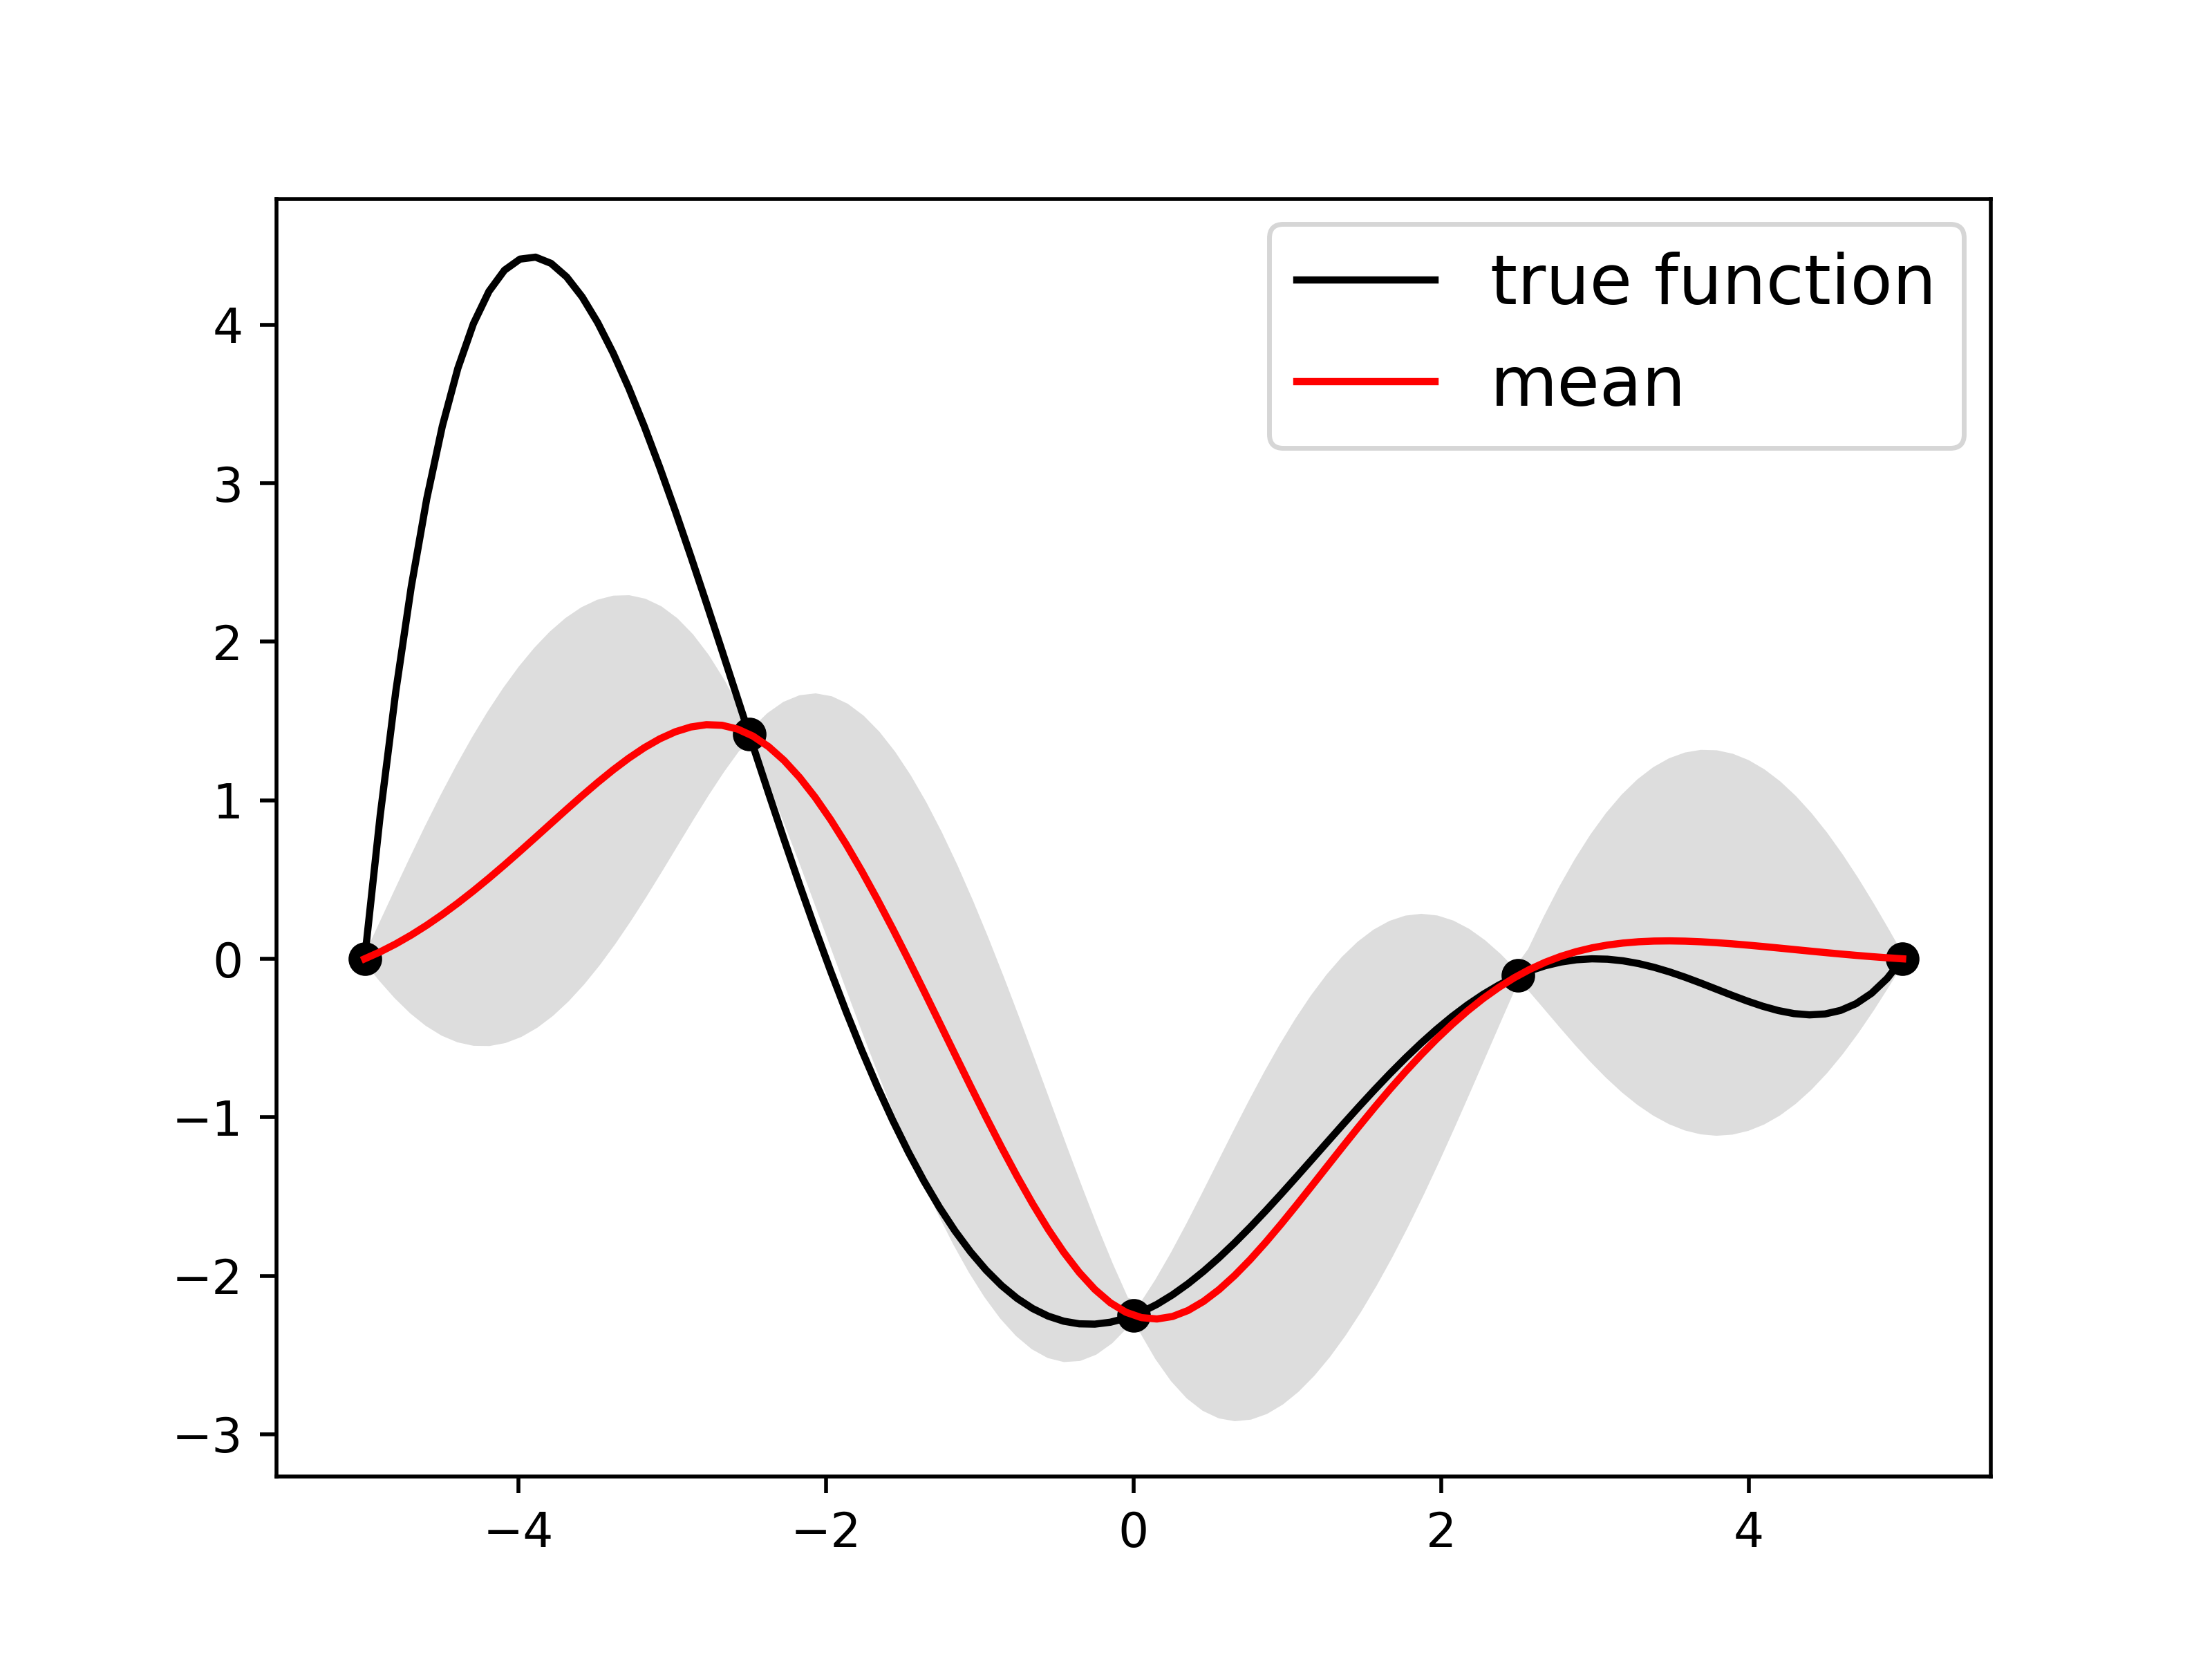
\includegraphics[scale=0.38]{figures/smooth-noder.png}
      \caption{\textbf{Function observations}}
    \end{subfigure}%
    \begin{subfigure}[b]{.5\textwidth}
      \centering
      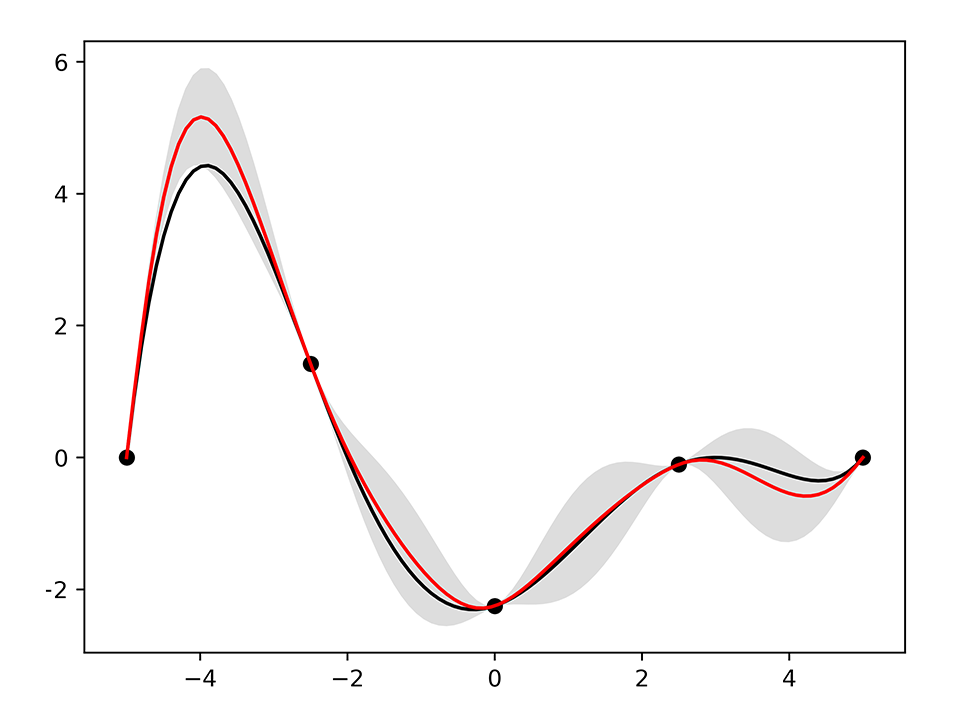
\includegraphics[scale=1.2]{figures/smooth-der.png}
      \caption{\textbf{Function and derivative observations}}
    \end{subfigure}
		\caption{Gaussian process approximations to a polynomial function using five regularly spaced inputs. The true function is shown in black and the GP is shown in red with 95\% confidence intervals in grey.}
		\label{smooth}
\end{figure}

Solak et al.~\cite{solak2003derivative} demonstrate reduced uncertainty and improved posterior mean accuracy under this model using derivative observations generated from local linearizations. Figure~\ref{smooth} presents an example of a GP approximation to an analytic function demonstrating these advantages with derivative observations obtained from automatic differentiation. The kernel used in Figure~\ref{smooth} and throughout this paper unless otherwise noted is the twice differentiable Mat\'ern kernel with smoothness parameter $\nu = 5/2$, given by
\begin{align*}
  k(\vec{x}, \tilde{\vec{x}}) = k_{\frac{5}{2}}\Big(Q(\vec{x}, \tilde{\vec{x}})^{1/2}\Big) & = \sigma^2 \Big(1 + \sqrt{5Q(\vec{x}, \tilde{\vec{x}})} + \frac{5}{3}Q(\vec{x}, \tilde{\vec{x}}) \Big) \exp\Big( - \sqrt{5Q(\vec{x}, \tilde{\vec{x}})} \Big) \\
  Q(\vec{x}, \tilde{\vec{x}}) & = (\vec{x} - \tilde{\vec{x}})^\top \Gamma^{-1} (\vec{x} - \tilde{\vec{x}}),
\end{align*}
where $\sigma^2$ is a noise parameter and $\Gamma = \diag\{\gamma_1,...,\gamma_p\}$ is a matrix of parameters $\gamma_k > 0$. In GP literature, $k(\cdot, \cdot)$ is often parameterized by \textit{length scales} $\ell_k = \sqrt{\gamma_k}$ for $k=1,...,p$, a convention we will also use.
The above kernel is an easily computable special case of the general Mat\'ern kernel
$$ k(\vec{x}, \tilde{\vec{x}}) = k_\nu \Big(Q(\vec{x}, \tilde{\vec{x}})^{1/2}\Big) = \sigma^2 \frac{2^{1-\nu}}{\Gamma(\nu)} \Big(\sqrt{2\nu Q(\vec{x}, \tilde{\vec{x}})}\Big)^\nu K_\nu\Big(\sqrt{2\nu Q(\vec{x}, \tilde{\vec{x}})}\Big), $$
where $K_\nu$ is the modified Bessel function of the second kind with order $\nu > 0$ and the quadratic form $Q(\vec{x}, \tilde{\vec{x}})$ is defined as above. The parameter $\nu$ varies the differentiability of the process, as its sample functions are $\floor{\nu-1}$-times differentiable. The Mat\'ern class contains as special cases the exponential kernel
$k(\vec{x}, \tilde{\vec{x}}) = \sigma^2 \exp(-\norm{\vec{x} - \tilde{\vec{x}}}_\Gamma)$ for $\nu = 1/2$, which has continuous but nondifferentiable sample paths, and the squared exponential kernel $k(\vec{x}, \tilde{\vec{x}}) = \sigma^2 \exp(-\norm{\vec{x} - \tilde{\vec{x}}}_\Gamma^2)$
taking $\nu \to \infty$, which has infinitely differentiable sample paths. The Mat\'ern kernel is referred to as \textit{stationary}, as it can be written as a function of the quadratic form $Q(\vec{x}, \tilde{\vec{x}})$ only, and does not depend on the location of $\vec{x}$ or $\tilde{\vec{x}}$ in $\Omega$.

It is important to reiterate that derivative interpolation is possible only for kernels which are at least twice differentiable. However, using such a kernel may induce a level of smoothness in the approximation which does not match the smoothness of the true function, as is the case near kinks in continuous piecewise smooth functions. Figure~\ref{kink} presents an example function for which derivative interpolation near a kink produces extraneous oscillation in the mean with low uncertainty. Figure~\ref{kink:short} demonstrates that if we reduce the global length scale of the process, this oscillation persists and the approximation deteriorates away from the kink. This motivates the introduction of nonstationary effects near kinks as discussed in Section~\ref{using_branch}.

Our main objective is to maintain the high accuracy of gradient-interpolating GPs in smooth regions while improving the approximation near kinks such that its mean does not suffer from oscillation and its variance is a good estimator of the true error. We now discuss a method for approximating the distance to potential kinks in functions evaluated by a computer code and present four GP constructions which use this distance to improve our approximation.

\begin{figure}[H]
		\centering
		\captionsetup{justification=centering}
    \begin{subfigure}[t]{.33\textwidth}
      \centering
      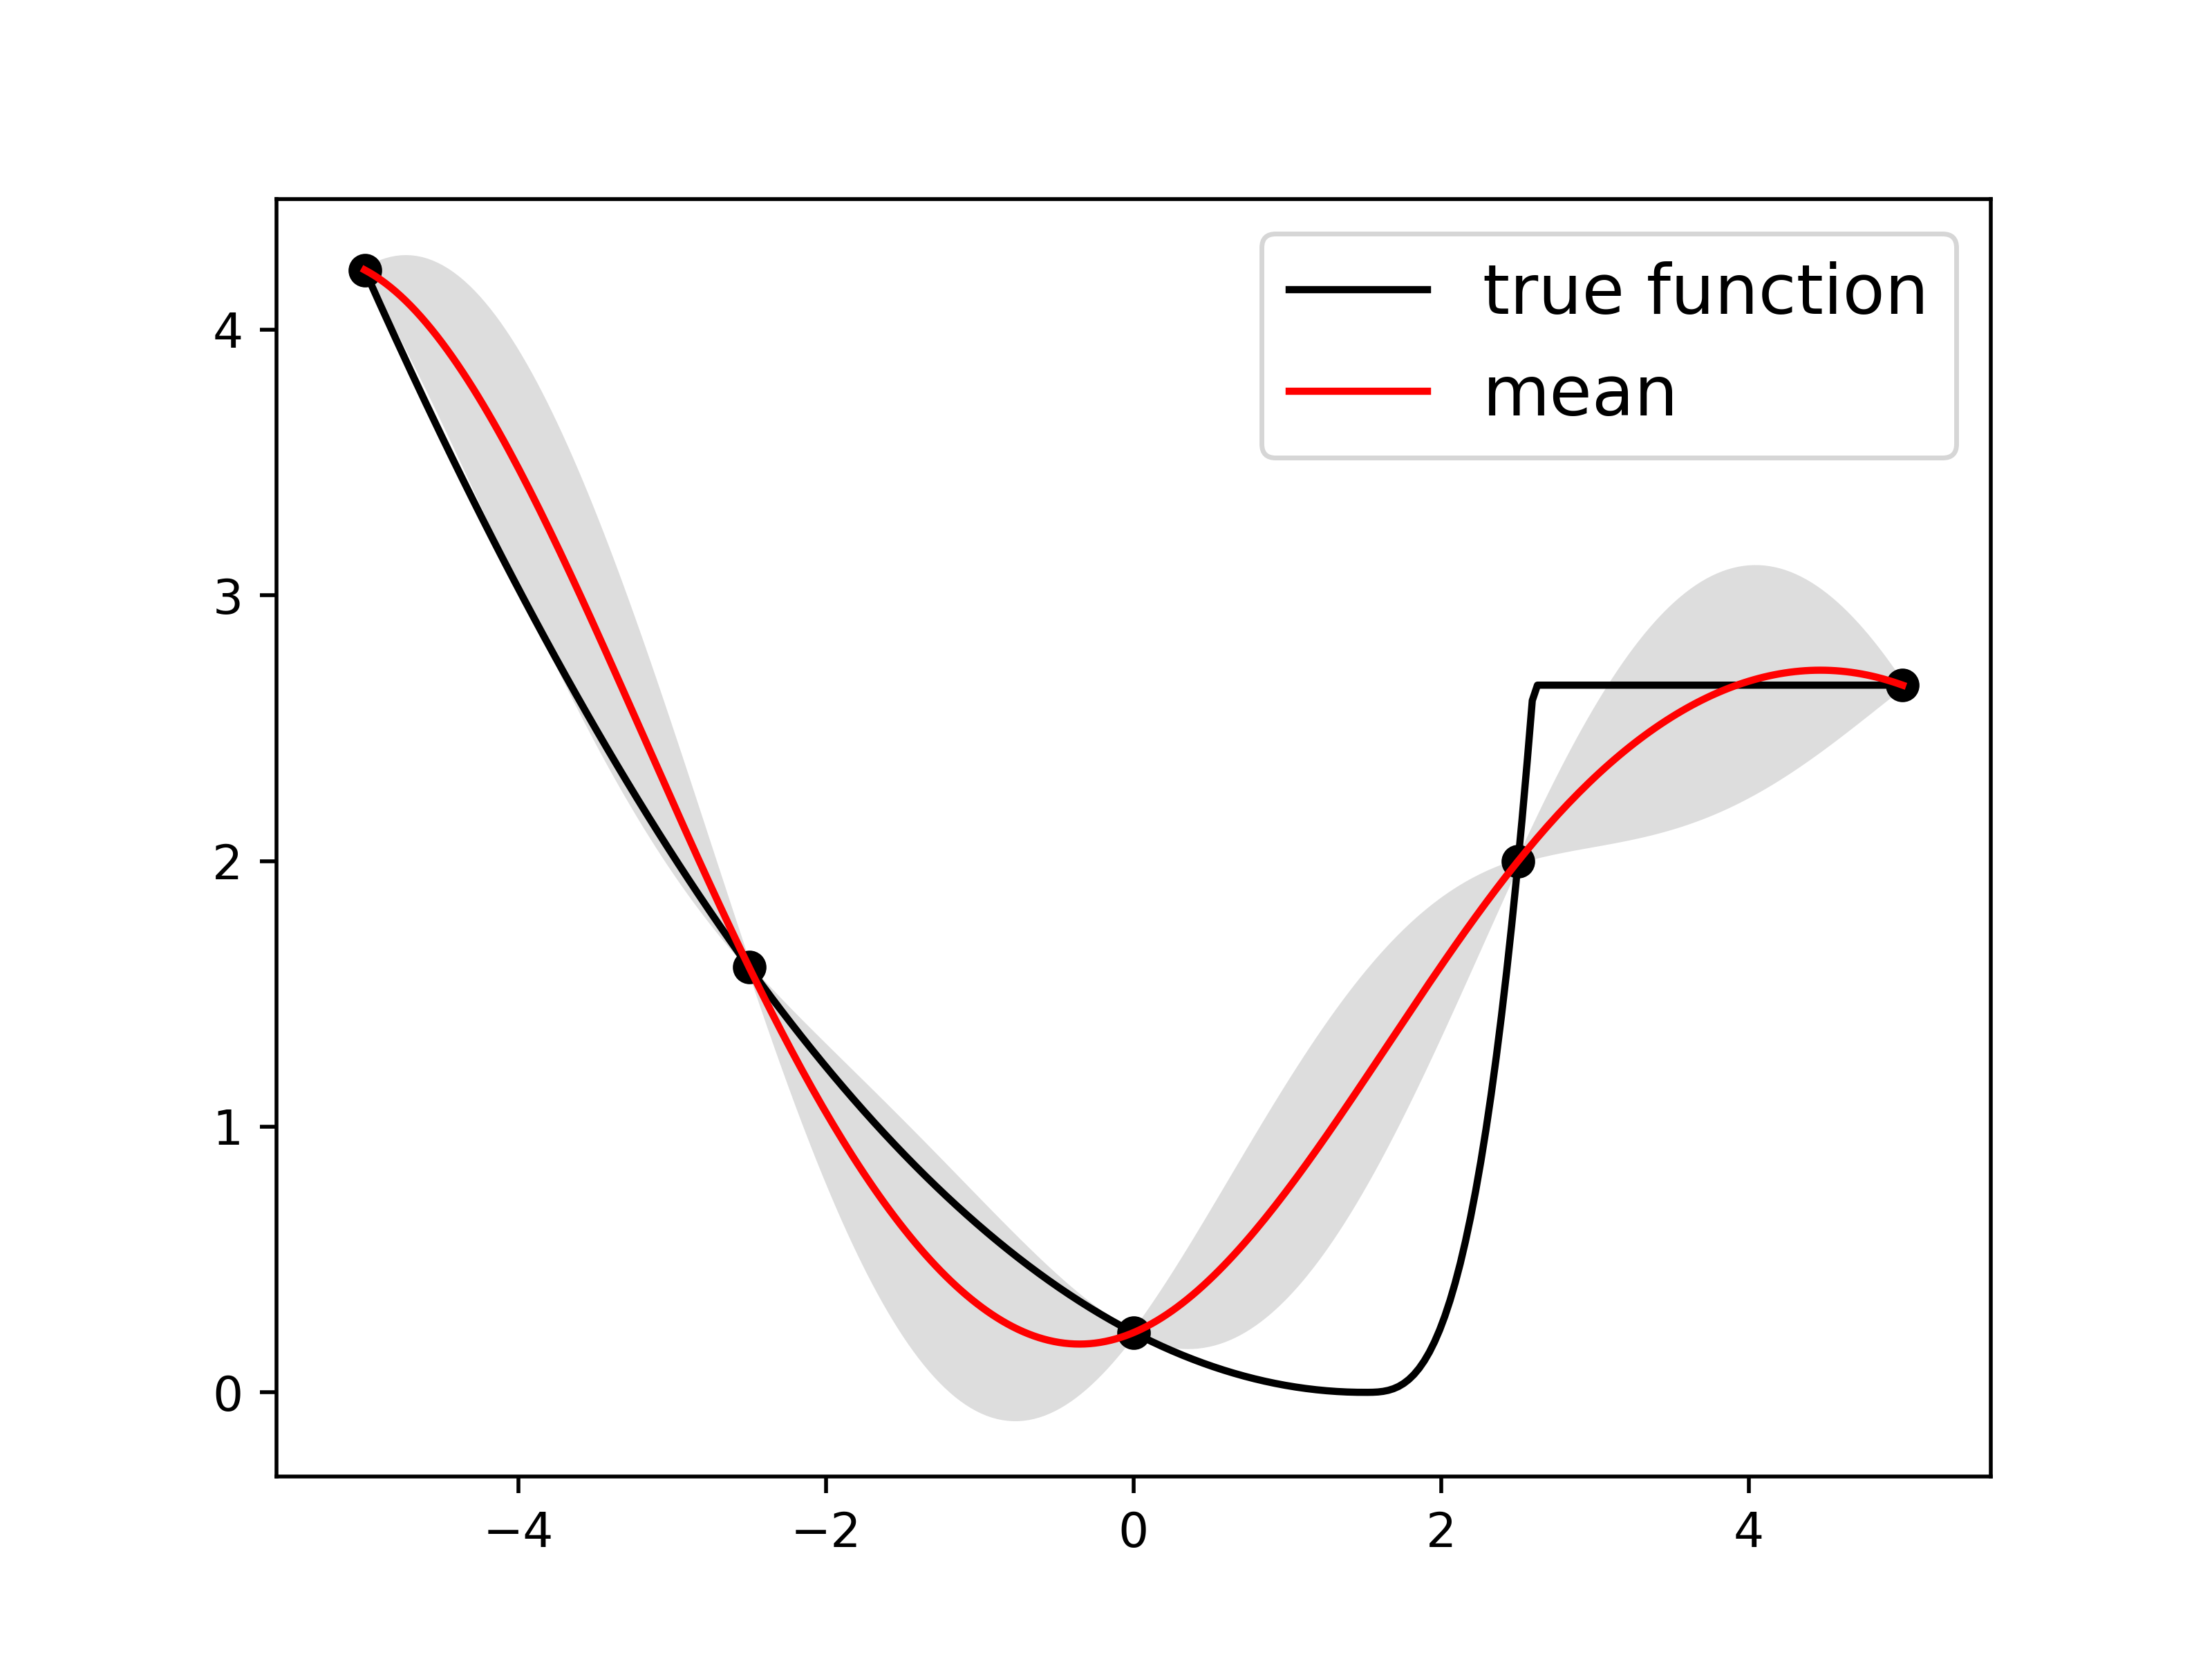
\includegraphics[scale=0.35]{figures/kink-noder.png}
      \caption{\textbf{Function observations} \\ $\ell = 3$}
    \end{subfigure}%
    \begin{subfigure}[t]{.33\textwidth}
      \centering
      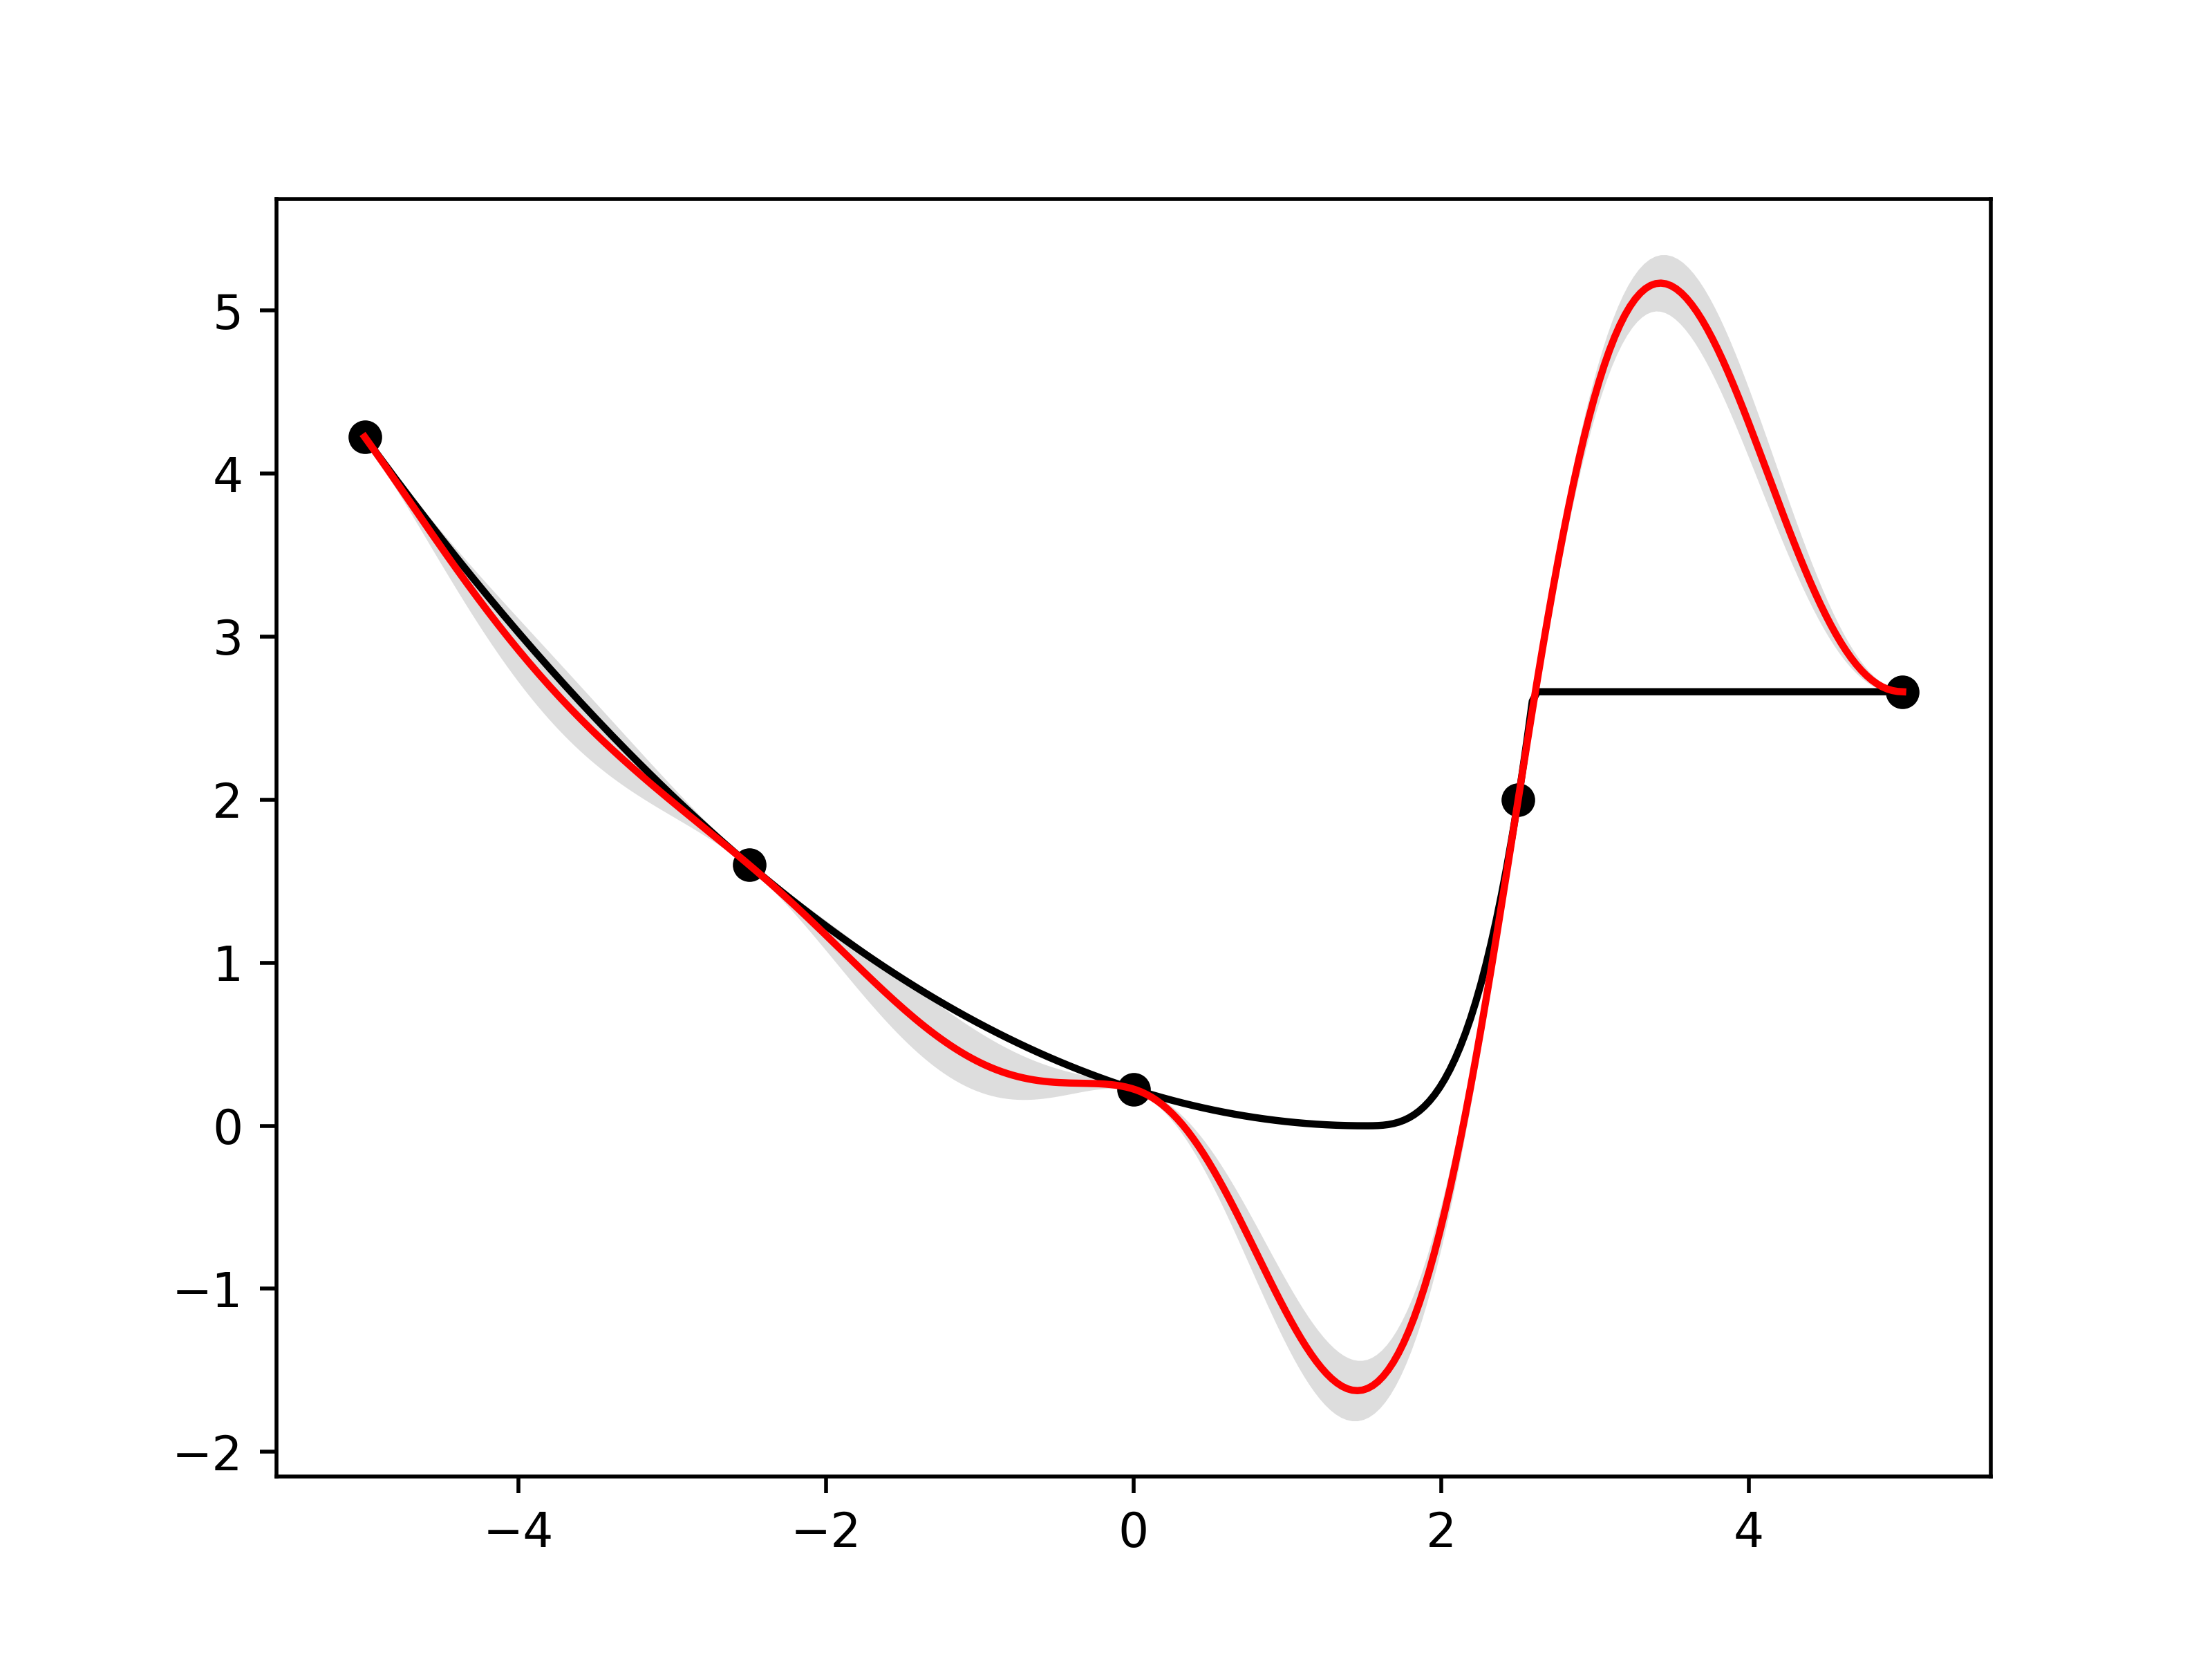
\includegraphics[scale=0.35]{figures/kink-der.png}
      \caption{\textbf{Function and derivative observations} \\ $\ell = 3$}
    \end{subfigure}%
    \begin{subfigure}[t]{.33\textwidth}
      \centering
      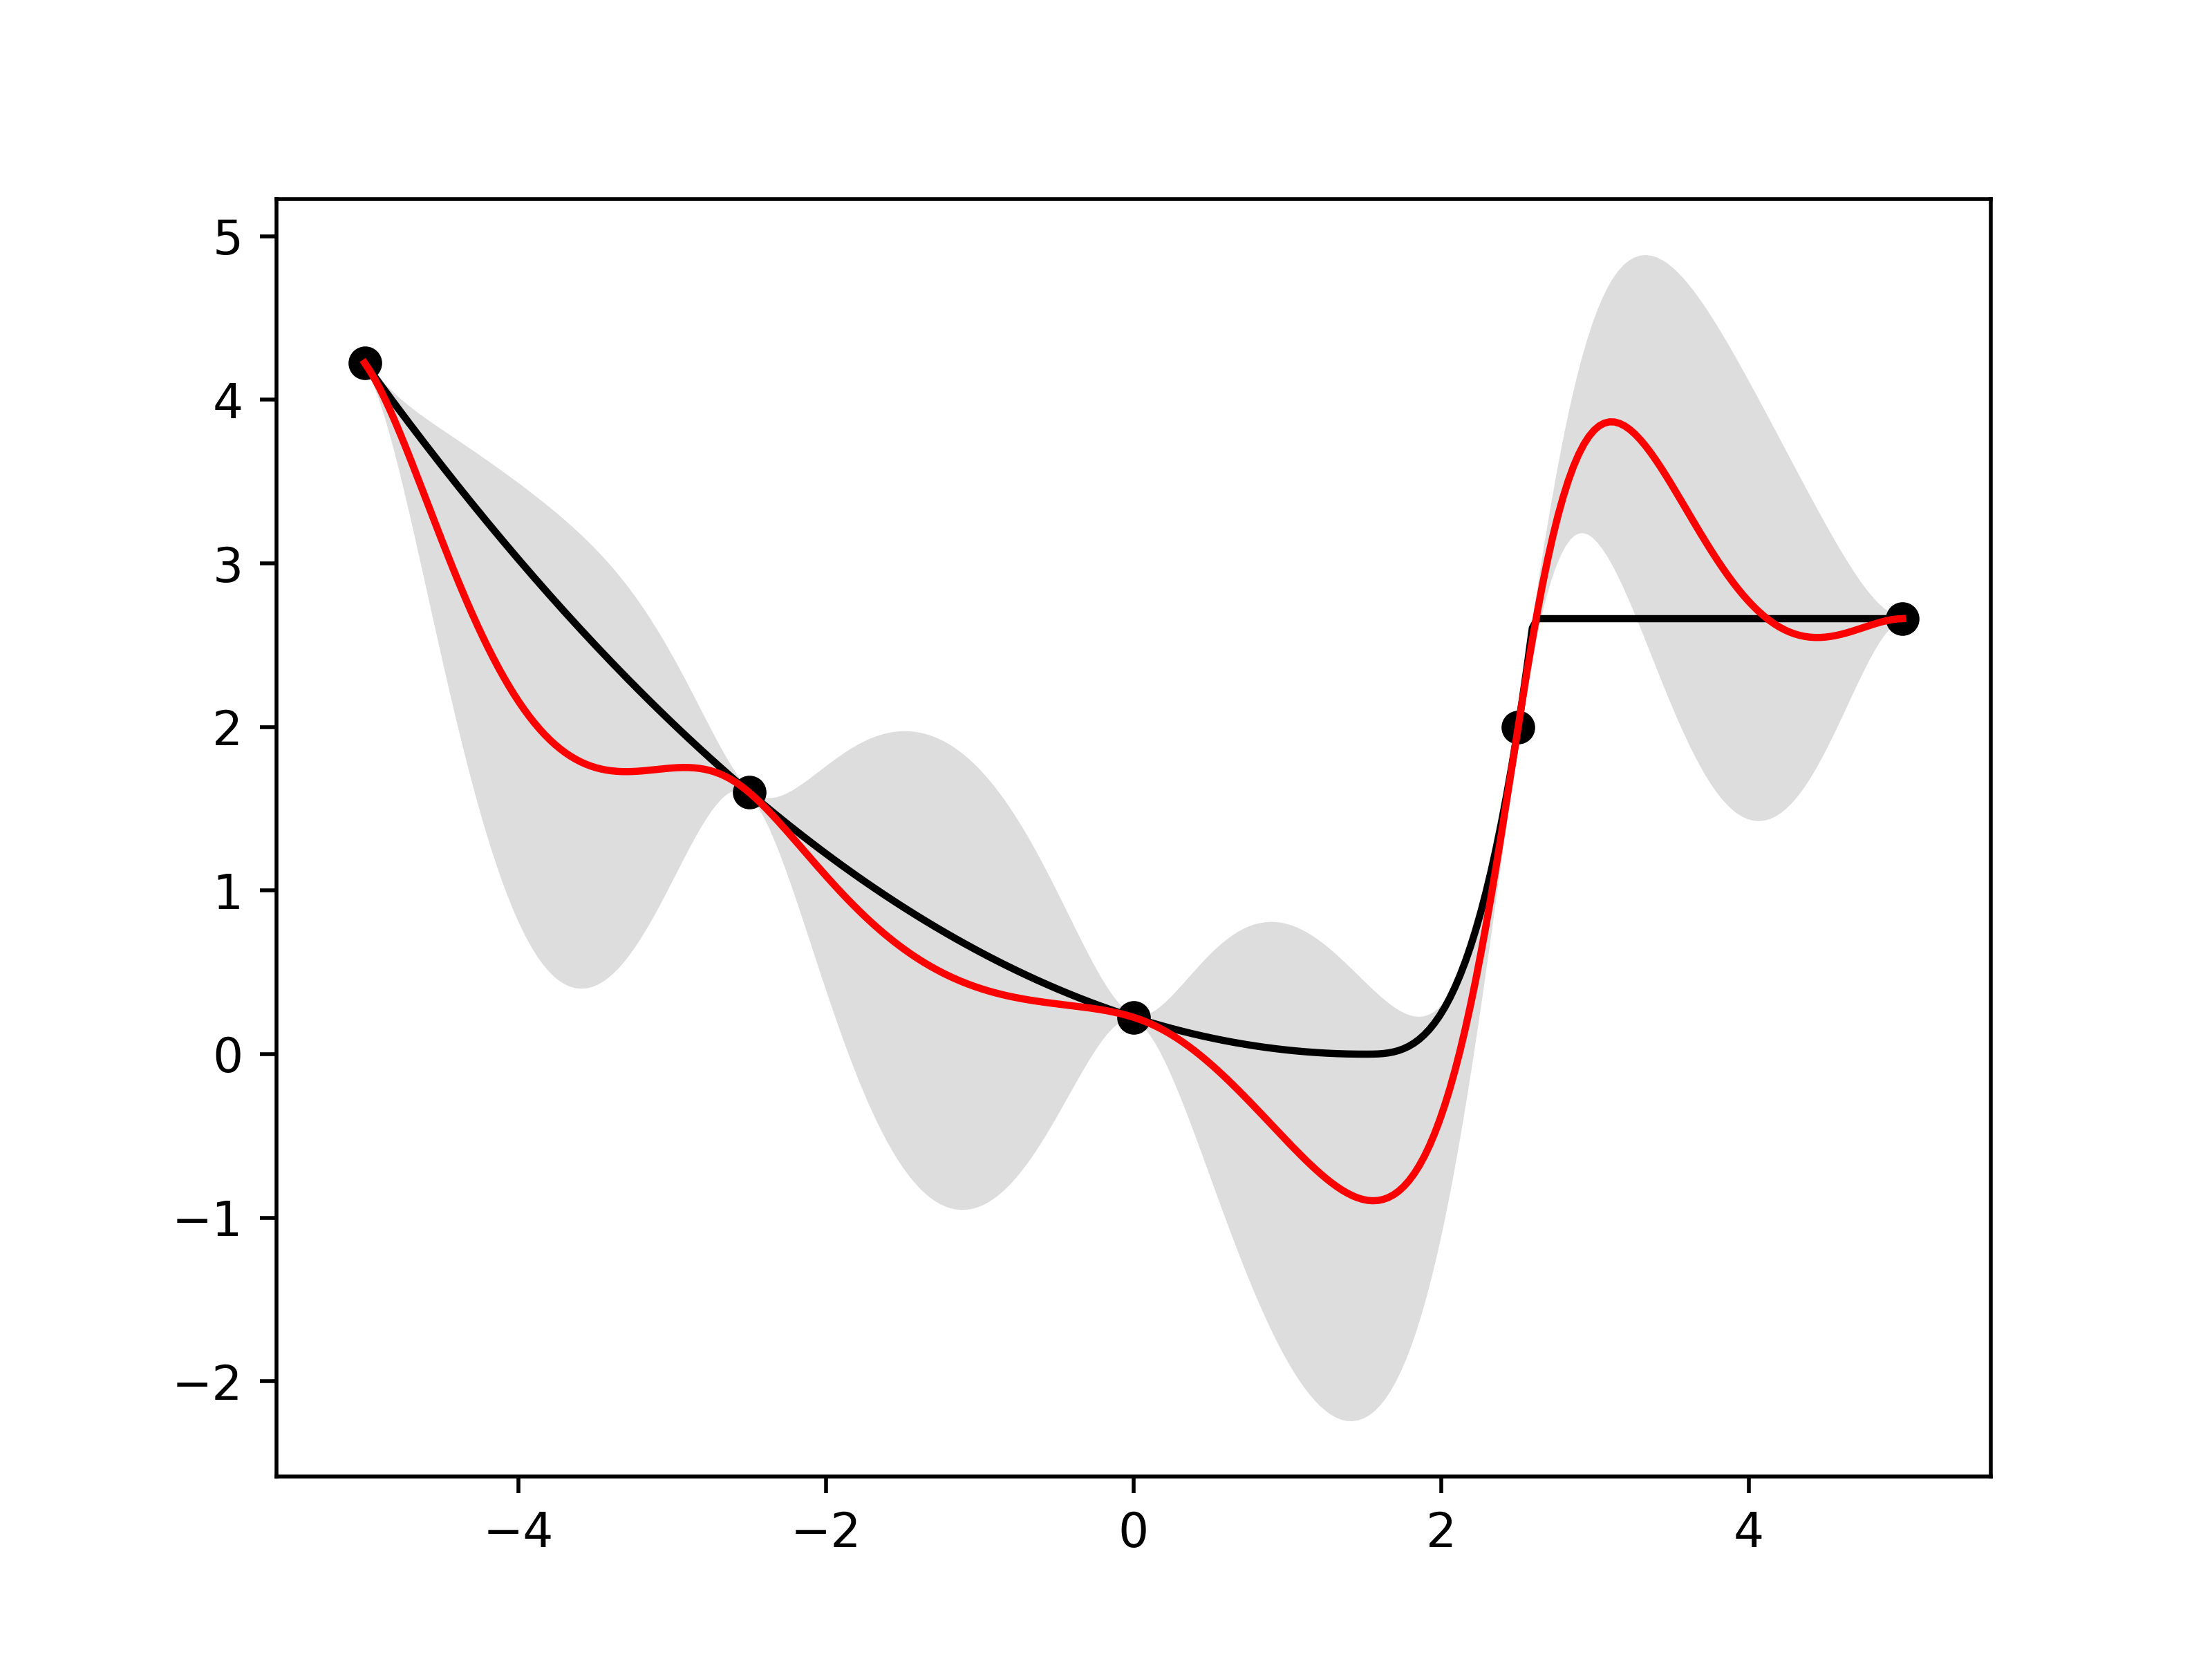
\includegraphics[scale=0.35]{figures/kink-shortder.png}
      \caption{\textbf{Function and derivative observations} \\ $\ell = 1$}
      \label{kink:short}
    \end{subfigure}
		\caption{Gaussian process approximations to a piecewise analytic function using five regularly spaced inputs with kernel length scale $\ell$.}
		\label{kink}
\end{figure}
\begin{algorithm}[H]
    \captionsetup{justification=centering}
    \begin{algorithmic}
    \IF{$g_1(\vec{x}) \geq 0$}
        \RETURN $2\cdot1.1^3$
    \ELSIF{$g_2(\vec{x}) \geq 0$}
        \RETURN $2(\vec{x}-1.5)^3$
    \ELSE
        \RETURN $0.1(\vec{x}-1.5)^2$
    \ENDIF
    \end{algorithmic}
    \caption{: $g_1(\vec{x}) = \vec{x}-2.6$, $g_2(\vec{x}) = \vec{x}-1.5$}
	\label{kink-code}
\end{algorithm}

\section{Branching functions}
We assume that the computer code used to evaluate $f$ is piecewise analytic on a compact set $\Omega \in \R^p$ with kinks occurring only at branching points in the code. We formulate these branching points as conditional statements of the form $g_j(\vec{x}) \geq 0$ for $j=1,...,m$. For example, Algorithm~\ref{kink-code} shows one way to write the function used in Figure~\ref{kink}. This branching structure divides the input space into disjoint computational subdomains on which the function is smooth.

One method for GP approximation of piecewise smooth functions is to infer a nonlinear warping of the underlying space which expands high variance regions near kinks, constructing a GP approximation in the warped space~\cite{marmin2018warped, xiong2007non}. Alternatively, one can explicitly model the boundary of each computational subdomain. This has been done in prior work by dividing the input space into a treed hierarchy~\cite{gramacy2008bayesian} or into polyhedra using a Voronoi tessellation~\cite{kim2005analyzing}. However, these results are applied mainly to low-dimensional problems, as explicit warpings and domain boundaries become difficult to estimate in higher dimensions, especially when computational complexity limits the sample size. Fiege et al.~\cite{fiege2018algorithmic} also address approximation and optimization of piecewise smooth functions by constructing local linearizations of $f$ using its gradient on each subdomain. However, their methods require that all kinks in the function are generated by the absolute value function and are thus not applicable to our more general computational model.

We estimate the branching distance $b_k(\vec{x})$ in each coordinate direction $k=1,...,p$ by constructing local linear approximations to the conditional functions $g_j(\vec{x})$ using gradients obtained by automatic differentiation. Take $\tilde{\vec{x}}$ such that $g_j(\tilde{\vec{x}}) = 0$. Then for each branching function $g_j(\vec{x})$, we have the linear approximation
$$ g_j(\vec{x}) = \nabla g_j(\vec{x})^\top (\vec{x} - \tilde{\vec{x}}). $$
Moving only in the $k^{th}$ coordinate direction between $\vec{x}$ and $\tilde{\vec{x}}$, we have
$$ \hat{b}_{k,j}(\vec{x}) = \abs{\vec{x}_k - \tilde{\vec{x}}_k} = \abs{\bigg(\frac{\partial g_j(\vec{x})}{\partial x_k}\bigg)^{-1} g_j(\vec{x})}. $$
Our approximate branching distance in direction $k$ is then given by
$$ \hat{b}_k(\vec{x}) = \min_{j=1,...,m} \hat{b}_{k,j}(\vec{x}). $$
Figure~\ref{branch} shows a two-dimensional example of this construction. Beyond its generality, there are two additional advantages of this approach over that of Fiege et al. First, while they compute the gradient of $f$ on each subdomain, which requires $2^m$ gradient computations, our method requires us only to compute the gradient of each of the $m$ branching functions. Second, branching functions and their gradients are likely to be less complex than $f$ itself, resulting in less expensive gradient computations. In addition, if the branching functions are linear, that is if the computational subdomains are polyhderal, then our linear approximations are exact. Polyhderal subdomains are more common in computer codes of interest than linear functions, and thus linearizing the function itself is much less likely to lead to globally accurate region boundaries.

\begin{figure}
		\centering
		\captionsetup{justification=centering}
		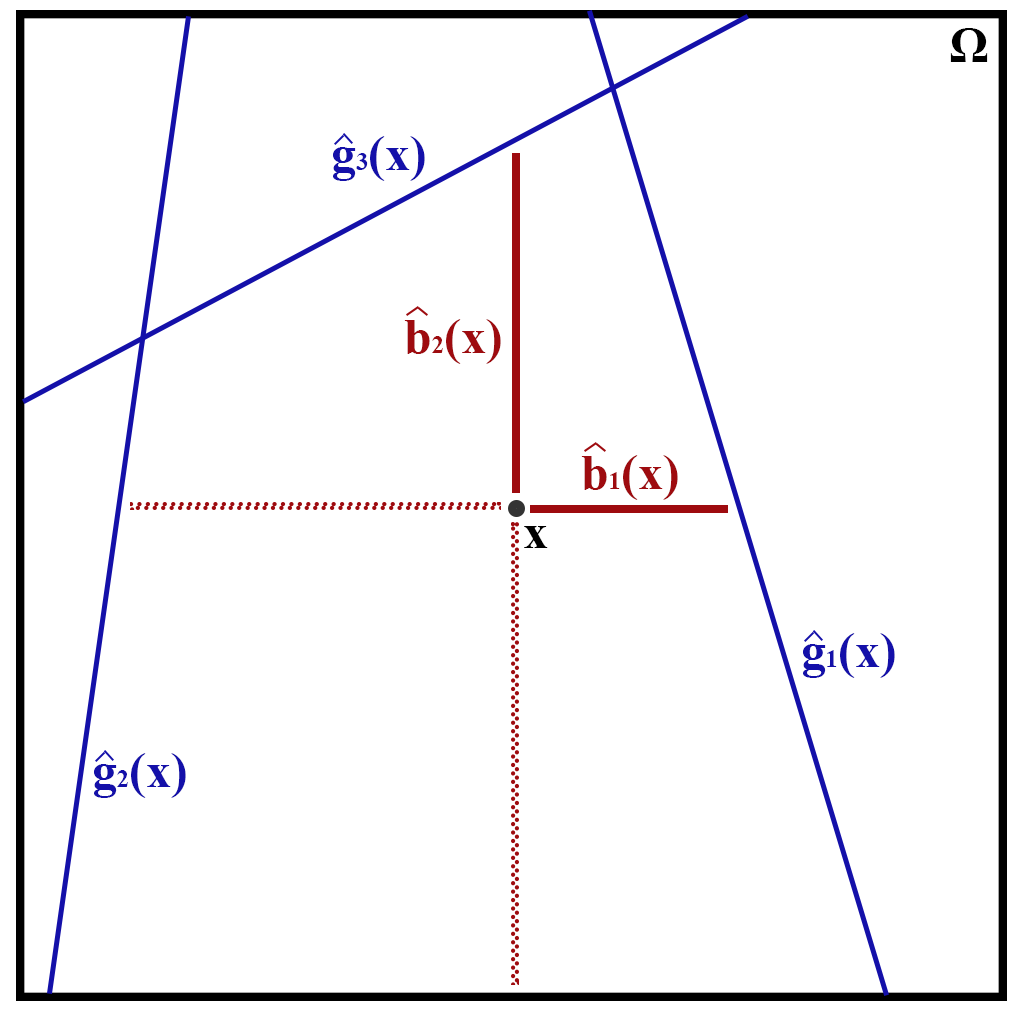
\includegraphics[scale=0.7]{figures/branch-approx.png}
		\caption{Local approximation to the branching distance in each coordinate direction. Blue lines show the intersection of the zero plane with the tangent plane to $g_j(\vec{x})$ at the point $\vec{x}$. Solid red lines show the minimum distance to such an intersection, which are used as the branching distances $\hat{b}_k(\vec{x})$. Dotted red lines show the distance to farther branches or the boundary of $\Omega$, which are not used.}
		\label{branch}
\end{figure}

\section{Using branching distance estimates} \label{using_branch}
While the Mat\'ern kernel used thus far is stationary, the branching domain boundaries with which we are concerned exist at specific locations in the input space. This suggests the use of a nonstationary process whose characteristics vary over the input space $\Omega$ depending on the estimated branching distance. We now develop and compare GP methods which use branching distance data to introduce various nonstationary effects.
\subsection{Nonstationary smoothness}
If we knew the exact location of all kinks in our function, then in order to obtain a GP with sample path differentiability which everywhere matches the differentiability of the true function, we would use a continuous but nondifferentiable kernel in the neighborhood of a kink and an infinitely differentiable kernel elsewhere. A result by Stein~\cite{stein2005nonstationary} proves as a special case that the nonstationary Mat\'ern kernel for which the smoothness parameter $\nu(\vec{x})$ varies over the input space, given by
\begin{align*}
  k(\vec{x}, \tilde{\vec{x}})
  & = k_{\frac{\nu(\vec{x}) + \nu(\tilde{\vec{x}})}{2}}\Big(Q(\vec{x}, \tilde{\vec{x}})^{1/2}\Big) \\
  Q(\vec{x}, \tilde{\vec{x}}) & = (\vec{x} - \tilde{\vec{x}})^\top \Gamma^{-1} (\vec{x} - \tilde{\vec{x}})
\end{align*}
is a valid covariance function, where $k_\nu(\cdot)$ is the Mat\'ern kernel with differentiability parameter $\nu$. This kernel requires a local differentiability parameter $\nu(\vec{x})$ to be defined on all of $\Omega$. We use the form
\begin{equation}
  \nu(\vec{x}) = \frac{1}{2} \exp\bigg(\min_{k=1,...,p} \frac{\hat{b}_k(\vec{x})}{\beta} \bigg) \label{eq:smoothness},
\end{equation}
where $\beta$ is a parameter controlling the localization of the nonsmoothness near subdomain boundaries. This approach requires that $\hat{b}_k(\vec{x})$ be defined on all of $\Omega$ for each $k=1,...,p$, not just on the input set $X$ for which we estimate the branching distance by local linearizations. In addition, the true branching distance is everywhere nonnegative, and $\hat{b}_k(\vec{x})$ must be everywhere positive in order for $\nu(\vec{x})$ to be a valid differentiability parameter. For this purpose, we use the exponentiated posterior means of GPs on $\log \hat{b}_k(\vec{x}_i)$ for $\vec{x}_i \in X$ with $k=1,...,p$.

While this approach is attractive in that it can accuractely model the differentiability of the piecewise analytic functions with which we are concerned, it has a number of drawbacks for applications in computer code modeling. First, if $\frac{\nu(\vec{x}) + \nu(\tilde{\vec{x}})}{2} < 2$, then $k(x, \tilde{x})$ is not twice differentiable. Thus we cannot interpolate gradient observations $\nabla y$ or $\nabla \tilde{y}$ which we have assumed we can obtain from AD, and which would likely improve our approximation in smooth regions. In addition, the process mean and variance, being linear and quadratic functions of kernel values, are not differentiable in such regions, and thus conventional gradient-based methods cannot be used for sequential design or optimization. Finally, the differentiability of the process is necessarily isotropic, seen by the minimum over directional branching distances in our expression for $\nu(\vec{x})$. However, the true function may have no kink in one direction but be very near a kink in another direction. Ideally we could leverage the direction-dependent nature of our branching distance data $\hat{b}_k(\vec{x})$ in such cases. We now present a method which allows us to interpolate gradient observations in smooth regions while maintaining nonstationary smoothness.

\subsection{Mixture of Gaussian processes}
Another approach which generates an approximation which is nonsmooth near kinks and smooth elsewhere is based on a mixture of experts model~\cite{jacobs1991adaptive} including both smooth GP and nonsmooth GP experts, where the mixture is informed by the branching distance. Under the mixture of GP experts model discussed in Rasmussen~\cite{rasmussen2002infinite}, each observation $(\vec{x}_i, y_i)$ is given a label $c_i \in \Z$ indicating which GP will interpolate it. The likelihood is then given by a weighted sum of multivariate Gaussian densities over all label assignments
\begin{align*}
  p(\vec{y} | X) & = \sum_\vec{c} p(\vec{y} | X, \vec{c}) \ p(\vec{c} | X) \\
  & = \sum_\vec{c} \bigg[ \prod_{j} p(\{y_i : c_i = j \} | \{\vec{x}_i : c_i = j \}) \bigg] p(\vec{c} | X),
\end{align*}
where each $p(\{y_i : c_i = j \} | \{\vec{x}_i : c_i = j \})$ is the conventional GP posterior density and $p(\vec{c} | X)$ is the probability of a given labeling, known as the \textit{gating network}. The set of all label assignments is exponentially large, and thus prior approaches have determined labels using expectation maximization for finite experts~\cite{tresp2001mixtures} and Gibbs sampling~\cite{meeds2006alternative} or variational inference~\cite{yuan2009variational} for infinite expert models.

We construct a two-expert model where one expert uses the nondifferentiable exponential kernel and the other expert uses the twice differentiable Mat\'ern $\nu = 5/2$ kernel. We let $c_i=0$ indicate the nonsmooth expert and $c_i=1$ the smooth expert. If we follow Rasmussen's construction, dividing the observations into two disjoint subsets and interpolating each subset with a separate expert, then in order for the posterior mean of the mixture to interpolate observations, we must construct the gating network such that $p(c_i = j | x_i) \in \{0,1\}$ for $\vec{x}_i \in X$. Otherwise the posterior mean will be a linear combination of the means of the smooth and nonsmooth experts, only one of which interpolates the observation $(\vec{x}_i, y_i)$.

As the nonsmooth expert does not suffer from oscillation near kinks, we depart from the conventional mixture of experts model and allow the nonsmooth expert to interpolate all observations, generating an underlying nondifferentiable approximation to the function. Thus we need only require that $p(c_i = 0 | x_i) = 1$ for all $\vec{x}_i \in X$ such that $p(c_i = 0 | x_i) > 0$ in order for the posterior mean of the mixture to interpolate observations. Therefore, rather than inferring the labels from the data, we set a threshold $\varepsilon > 0$ and define the gating network for observations $(\vec{x}_i, y_i)$ by
\begin{equation}
  p(c_i = 0 | \vec{x}_i) = \left\{\begin{array}{lr}
          1 & \quad \text{for } \displaystyle\min_{k=1,...,p} \hat{b}_k(\vec{x}_i) < \varepsilon \\
          0 & \text{otherwise} \qquad
        \end{array} \right
\end{equation}
We extend this gating network to the entire input space $\Omega$ by
\begin{equation}
  p(c_* = 0 | \vec{x}_*) = s\Bigg(\min_{\substack{x_i \in X \\ c_i = 0}} \norm{\vec{x}_* - \vec{x}_i}\Bigg), \label{eq:gating}
\end{equation}
where $s: \R \to [0,1]$ is a smoothing function. For optimization applications, it is desirable for the posterior mean and variance to be nondifferentiable on a small, compact subset of $\Omega$ so that gradient-based methods can be used outside of this subset. Thus we would like $s(\cdot)$ to be compactly supported. We use the Wendland radial function~\cite{wendland1995piecewise, fasshauer1998smoothing}
$$ s(r) = \max\Big( 1-\frac{r}{\delta}, 0 \Big)^{\ell+1} \Big[(\ell + 1) \frac{r}{\delta} + 1\Big],$$
where $\ell = \floor{p/2} + 2$. This function is supported on the ball of radius $\delta$ in $\R^p$ and has $\floor{p/2} + 2$ continuous derivatives at $r = \delta$. This smoothness prevents extraneous kinks in the posterior mean at the boundary of the support of $s(\cdot)$. By enforcing a compact support on the probability of using the nonsmooth expert, our posterior mean can interpolate both gradient and function observations exactly using the smooth expert for most observations, mixing with the nonsmooth expert only where proximity to a kink may cause oscillation.

The primary disadvantage to this approach in applications is the nondifferentiability of the posterior mean near kinks. Although this property reduces oscillation and allows the posterior mean of the mixture to adapt to the differentiability characteristics of the true function, it introduces additional complexity into optimization and sequential design routines, as gradient methods cannot be used on certain compact subsets of the input space. In addition, gradient observations near kinks are completely disregarded. Although strict interpolation causes oscillation, these observations still carry valuable information regarding the local behavior of the true function. We may thus hope to incorporate gradient observations and mitigate oscillation issues with an alternative nonstationary effect. We now develop two methods which use all gradient observations and produce an everywhere differentiable approximation suitable for optimization.

\subsection{Nonstationary length scale}
One approach to reducing oscillation near kinks is to decrease the length scale of the process as we approach subdomain boundaries, localizing the oscillation effect to a small neighborhood of the kink. Paciorek and Schervish~\cite{paciorek2004nonstationary} generalize the nonstationary squared exponential kernel described in~\cite{gibbs1998bayesian}, providing a method for constructing a nonstationary kernel with varying anisotropic length scale from an arbitrary stationary kernel. Applied to the Mat\'ern kernel with local length scale matrices $\Gamma(\vec{x})$, this result gives
\begin{align*}
  k(\vec{x}, \tilde{\vec{x}})
  & = |\Gamma(\vec{x})|^{\frac{1}{4}} |\Gamma(\tilde{\vec{x}})|^{\frac{1}{4}} \abs{\frac{\Gamma(\vec{x}) + \Gamma(\tilde{\vec{x}})}{2}}^{-\frac{1}{2}}
  k_\nu \Big(Q(\vec{x}, \tilde{\vec{x}})^{1/2}\Big) \\
  Q(\vec{x}, \tilde{\vec{x}}) & = (\vec{x} - \tilde{\vec{x}})^\top \Big(\frac{\Gamma(\vec{x}) + \Gamma(\tilde{\vec{x}})}{2}\Big)^{-1} (\vec{x} - \tilde{\vec{x}})
\end{align*}
Assuming the matrices $\Gamma(\vec{x})$ are diagonal, we can efficiently compute
\begin{align*}
   |\Gamma(\vec{x})|^{\frac{1}{4}} |\Gamma(\tilde{\vec{x}})|^{\frac{1}{4}} \abs{\frac{\Gamma(\vec{x}) + \Gamma(\tilde{\vec{x}})}{2}}^{-\frac{1}{2}}
   & = 2^{p/2} \prod_{k=1}^p \frac{\gamma_k(\vec{x})^\frac{1}{4} \gamma_k(\tilde{\vec{x}})^\frac{1}{4}}{(\gamma_k(\vec{x}) + \gamma_k(\tilde{\vec{x}}))^\frac{1}{2}} \\
   (\vec{x} - \tilde{\vec{x}})^\top \Big(\frac{\Gamma(\vec{x}) + \Gamma(\tilde{\vec{x}})}{2}\Big)^{-1} (\vec{x} - \tilde{\vec{x}})
   & = 2 \sum_{k=1}^p \frac{(\vec{x}_k - \tilde{\vec{x}}_k)^2}{\gamma_k(\vec{x}) + \gamma_k(\tilde{\vec{x}})}
\end{align*}
This kernel requires local parameters
$\gamma_k(\vec{x})$ to be defined for each coordinate direction $j=k,...p$ on all of $\Omega$. We define a local length scale
\begin{equation}
  \sqrt{\gamma_k(\vec{x})} = \ell_k(\vec{x}) = (\ell_{max} - \ell_{min}) \bigg[1 - \exp\bigg(-\frac{\hat{b}_k(\vec{x})}{\beta}\bigg)\bigg] + \ell_{min}, \label{eq:length}
\end{equation}
where $\ell_{min}$ and $\ell_{max}$ are length scales between which $\ell_k(\vec{x})$ can vary, and $\beta$ is a parameter controlling the localization of length scale shortening near subdomain boundaries. As in the nonstationary smoothness approach, this method also requires that $\hat{b}_k(\vec{x})$ be defined on all of $\Omega$, not just on the input set $X$ for which we estimate the branching distance by local linearizations. In addition, $\hat{b}_k(\vec{x})$ must be everywhere positive and twice differentiable in order for $k(\cdot, \cdot)$ to be twice differentiable and for $\ell_k(\vec{x})$ to be a valid length scale. For this purpose, we use the exponentiated mean of a GP on
$\log \hat{b}_k(\vec{x}_i)$ for $\vec{x}_i \in X$ using the Mat\'ern $\eta = 5/2$ kernel. This GP approach to global length scale is similar to that of Plagemann et al.~\cite{plagemann2008nonstationary} who use the mean of a log GP as a nonstationary length scale, estimating it from observations instead of computing it directly using branching distance data.

There are a number of drawbacks to this approach. First, it is difficult to determine a form for $\ell_k(\vec{x})$ which sufficiently reduces oscillation without causing the mean of the process to tend too aggressively towards the prior mean zero near kinks. Our functional form works well for a number of test cases, but is heuristic. In addition, for each new observation we must compute the posterior mean of the directional branching distance GPs, which is an $O(n^3)$ operation for each $k=1,...,p$. Finally, the actual branching distance is a nondifferentiable piecewise linear function, and estimating such functions using a GP with twice-differentiable kernel is precisely the problem with which we are concerned in this paper. Thus the approximation may suffer from inaccuracy. We now discuss an alternative method which does not rely on a global approximation to the branching distance.

\subsection{Nonstationary additive derivative noise} \label{ADN}
We now introduce a novel model which adds independent mean zero Gaussian noise to derivative observations near branching points. The nonstationary length scale method above interpolates gradient observations exactly and attempts to reduce oscillation by localizing the covariance effects of gradient observations near kinks. However, we can avoid oscillation while maintaining the global length scale if we do not interpolate gradient observations exactly. We do so using additive noise to encode our uncertainty about gradient observations in the neighborhood of a kink. Intuitively, gradients can change severely as we pass from one branching domain to another, and thus we should trust gradient observations near branching points less than those in smooth regions. Introducing Gaussian noise with variance $\sigma^2_k(\vec{x}_i)$ to derivative observation $\frac{\partial y_i}{\partial x_k}$ gives
$$ \Cov\Big(\frac{\partial y_i}{\partial x_k}, \frac{\partial y_i}{\partial x_k}\Big) = \frac{\partial^2}{\partial x_k^2} k(\vec{x}_i, \vec{x}_i) + \sigma^2_k(\vec{x}_i). $$
Applied to all derivative observations, this amounts to adding a diagonal matrix
$$\Sigma(X) = \diag\{\sigma^2_1(\vec{x}_1),...,\sigma^2_p(\vec{x}_1),...,\sigma^2_1(\vec{x}_n),...,\sigma^2_p(\vec{x}_n)\}$$
to the lower right block $\nabla^2 K$ of the covariance matrix $\bar{K}$ given in equation \ref{eq:K_bar}. The covariance matrix with additive derivative noise is then given by
$$ \bar{K}_\sigma = \mat{K & \nabla K \\ \nabla K^\top & \nabla^2 K + \Sigma(X)}. $$
We construct a functional form for the noise based on the estimated branching distance
\begin{equation}
  \sigma^2_k(\vec{x}_i) = \sigma^2_{max} \exp\bigg(- \frac{\hat{b}_k(\vec{x}_i)}{\beta}\bigg), \label{eq:noise}
\end{equation}
where $\beta$ controls the localization of noise and $\sigma_{max}^2$ controls the maximum noise. Note that we do not need a global approximation to the branching distance. We require only the estimates already obtained for $\vec{x}_i \in X$.

To understand the behavior of this process, consider adding Gaussian noise with variance $\sigma^2$ to $\frac{\partial y_i}{\partial x_k}$, the $k^{th}$ partial derivative observation at input $\vec{x}_i$. Let $s = n + p \cdot (i-1) + k$ be the row and column index of this covariance in the matrix $\bar{K}$. The Sherman-Morrison formula then gives the inverse covariance matrix
\begin{align*}
  \Big(\bar{K} + \sigma^2 e_s e_s^\top\Big)^{-1}
  & = \bar{K}^{-1} - \frac{\sigma^2}{1 + \sigma^2 e_s^\top \bar{K}^{-1} e_s} \bar{K}^{-1} e_s e_s^\top \bar{K}^{-1} \\
  & = \bar{K}^{-1} \Bigg(I - \frac{\sigma^2}{1 + \sigma^2 (\bar{K}^{-1})_{ss}} \mat{0 & & 0 \\ (\bar{K}^{-1})_{s1} & ... & (\bar{K}^{-1})_{s,n(p+1)} \\ 0 & & 0} \Bigg) \\
  & \to \bar{K}^{-1} \mat{ I & 0 & 0 \\ \frac{-1}{(\bar{K}^{-1})_{ss}}(\bar{K}^{-1})_{s,1:(s-1)} & 0 & \frac{-1}{(\bar{K}^{-1})_{ss}}(\bar{K}^{-1})_{s,(s+1):n(p+1)} \\ 0 & 0 & I } \\
  \text{as} \quad \sigma^2 & \to \infty
\end{align*}
Thus as $\sigma^2_k(\vec{x}_i)$ increases, the contribution of terms involving $\frac{\partial y_i}{\partial x_k}$ in the posterior mean \eqref{eq:posterior-mean-der} vanishes, and the GP posterior variance \eqref{eq:posterior-var-der} is already independent of function and gradient observations. In particular, in the limit $\sigma^2_k(\vec{x}_i) \to \infty$
for all $k=1,...,p$ and $i=1,...,n$ we obtain the GP interpolating only function value observations and ignoring gradient observations. Clearly we obtain a gradient-interpolating GP as $\sigma^2_k(\vec{x}_i) \to 0$. Therefore adding nonstationary noise to gradient observations depending on the estimated branching distances allows us to effectively mix between function-interpolating and gradient-interpolating processes in each coordinate direction over the input space depending on how close we are to a kink.

\begin{figure}
		\centering
		\captionsetup{justification=centering}
    \begin{subfigure}[b]{.4\textwidth}
      \centering
      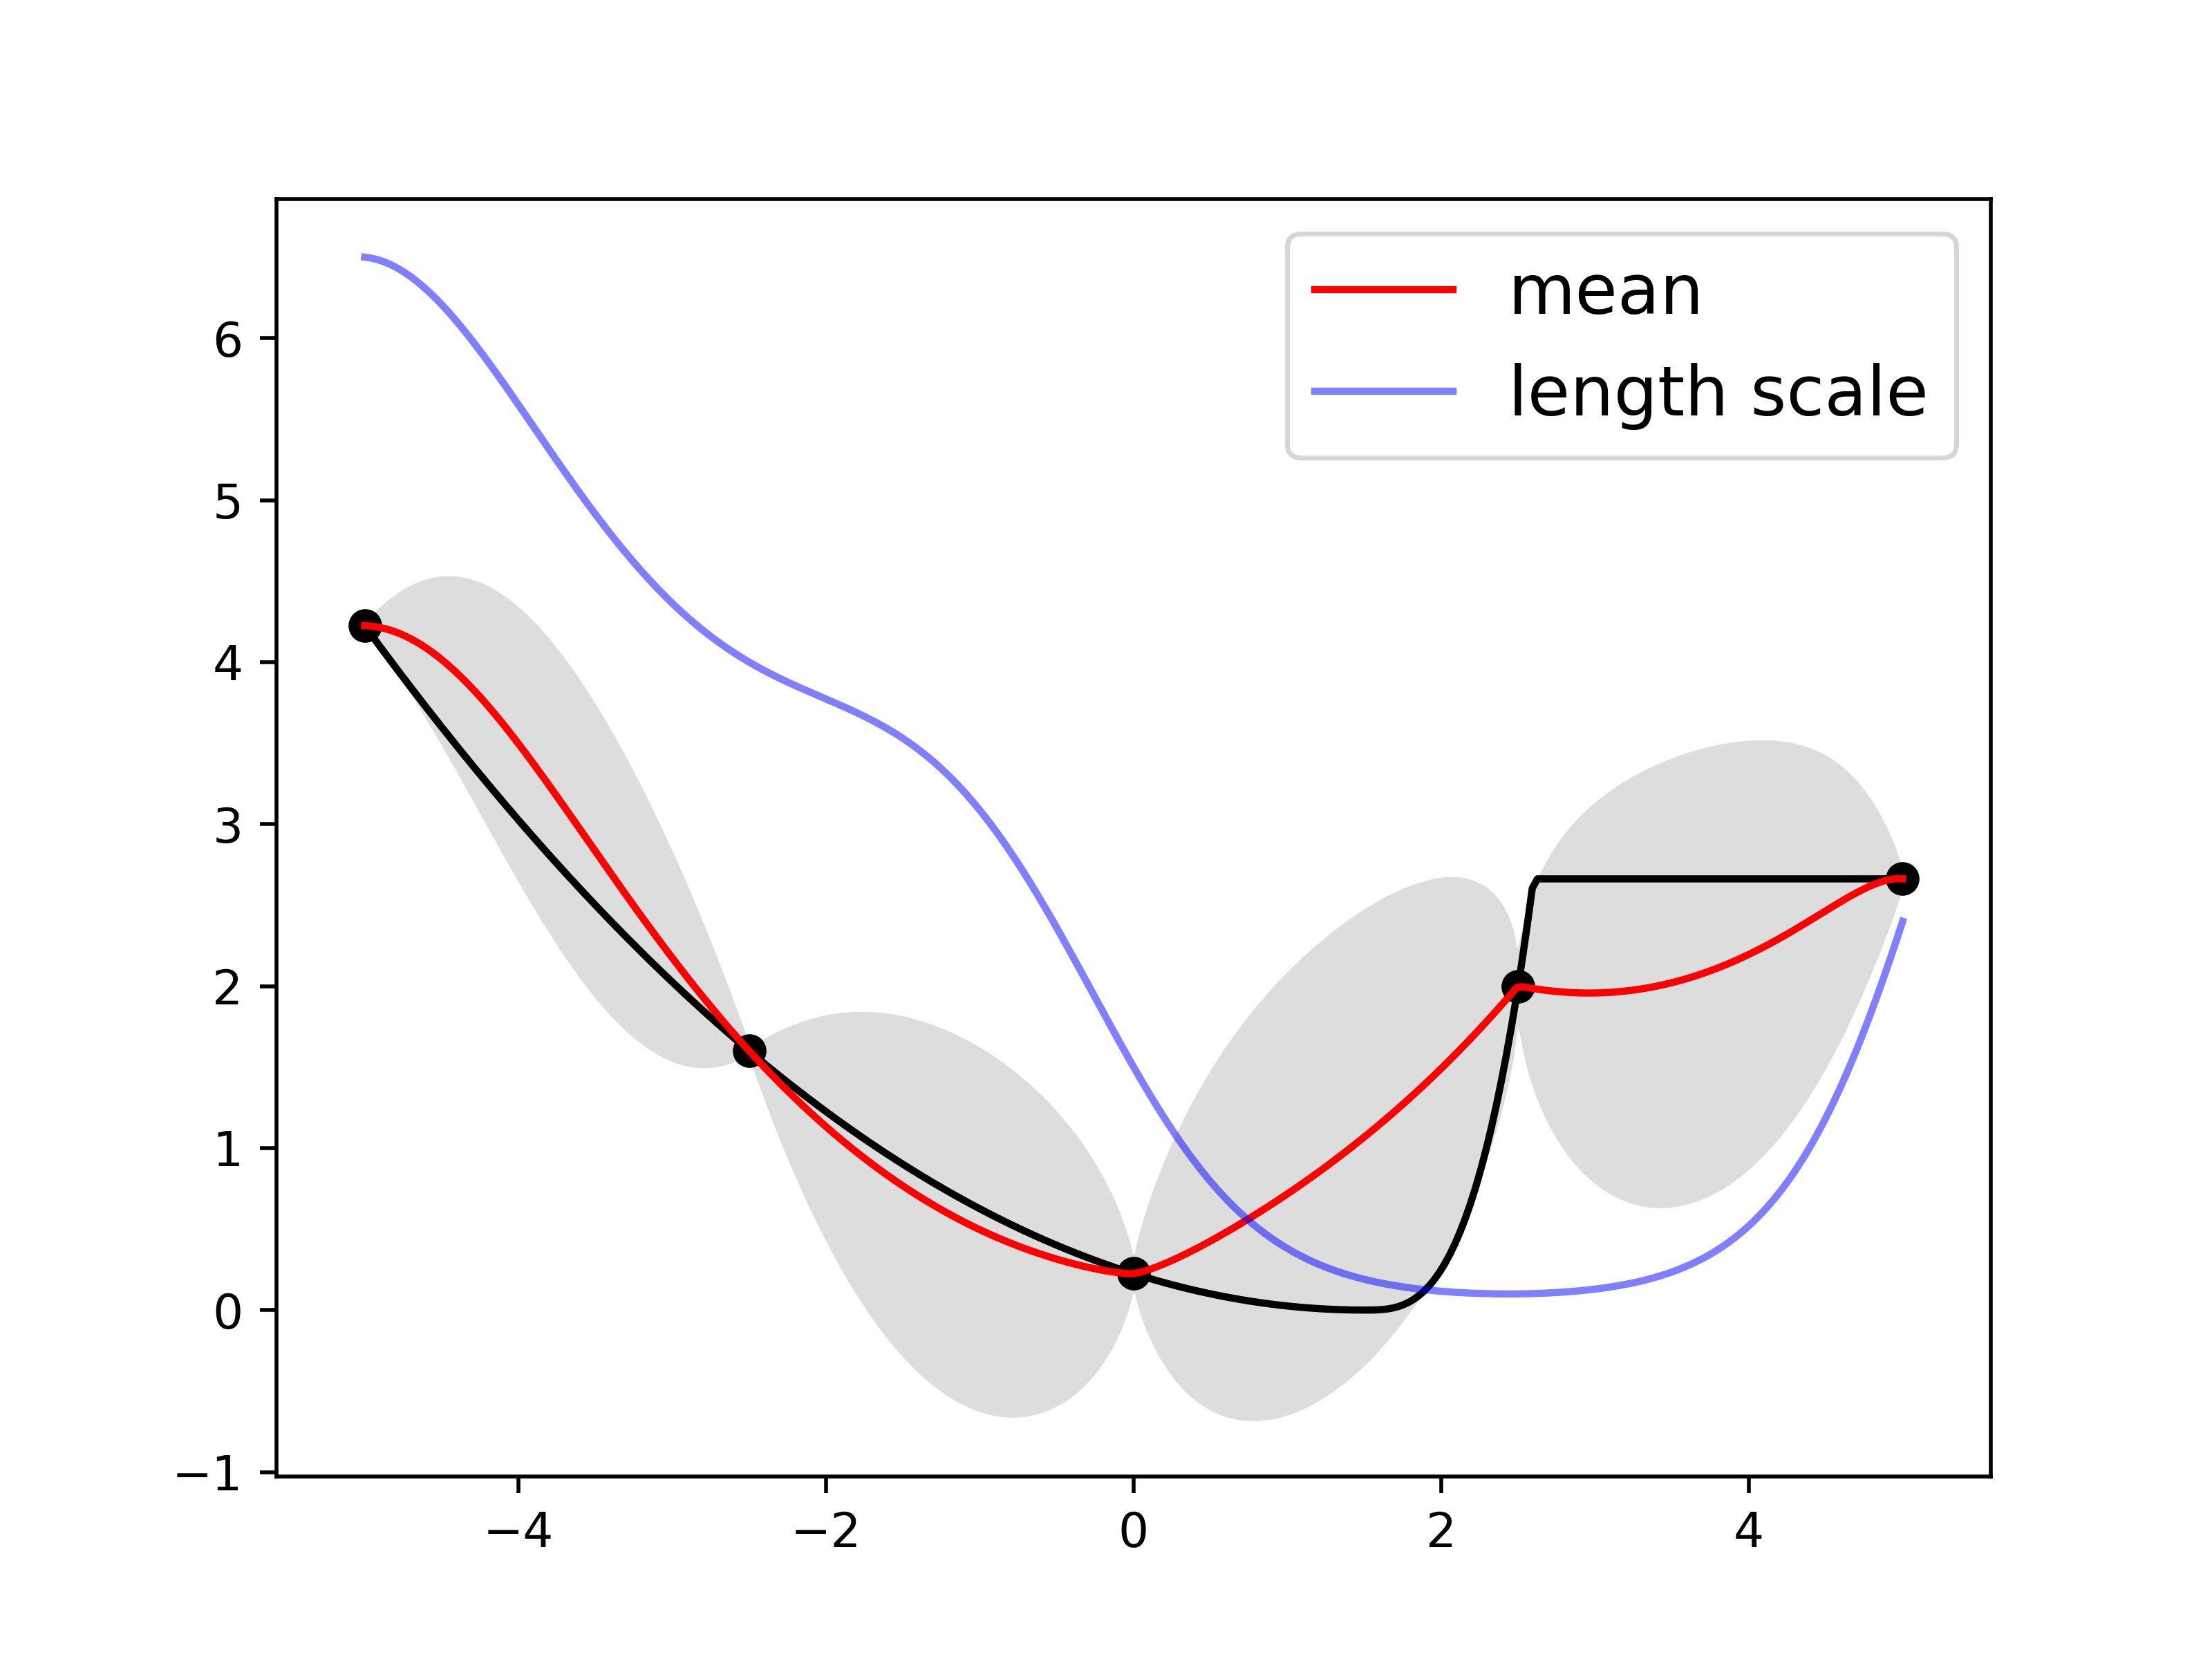
\includegraphics[scale=0.35]{figures/kink-smoothness.png}
      \caption{\textbf{Nonstationary smoothness}}
    \end{subfigure}%
    \begin{subfigure}[b]{.4\textwidth}
      \centering
      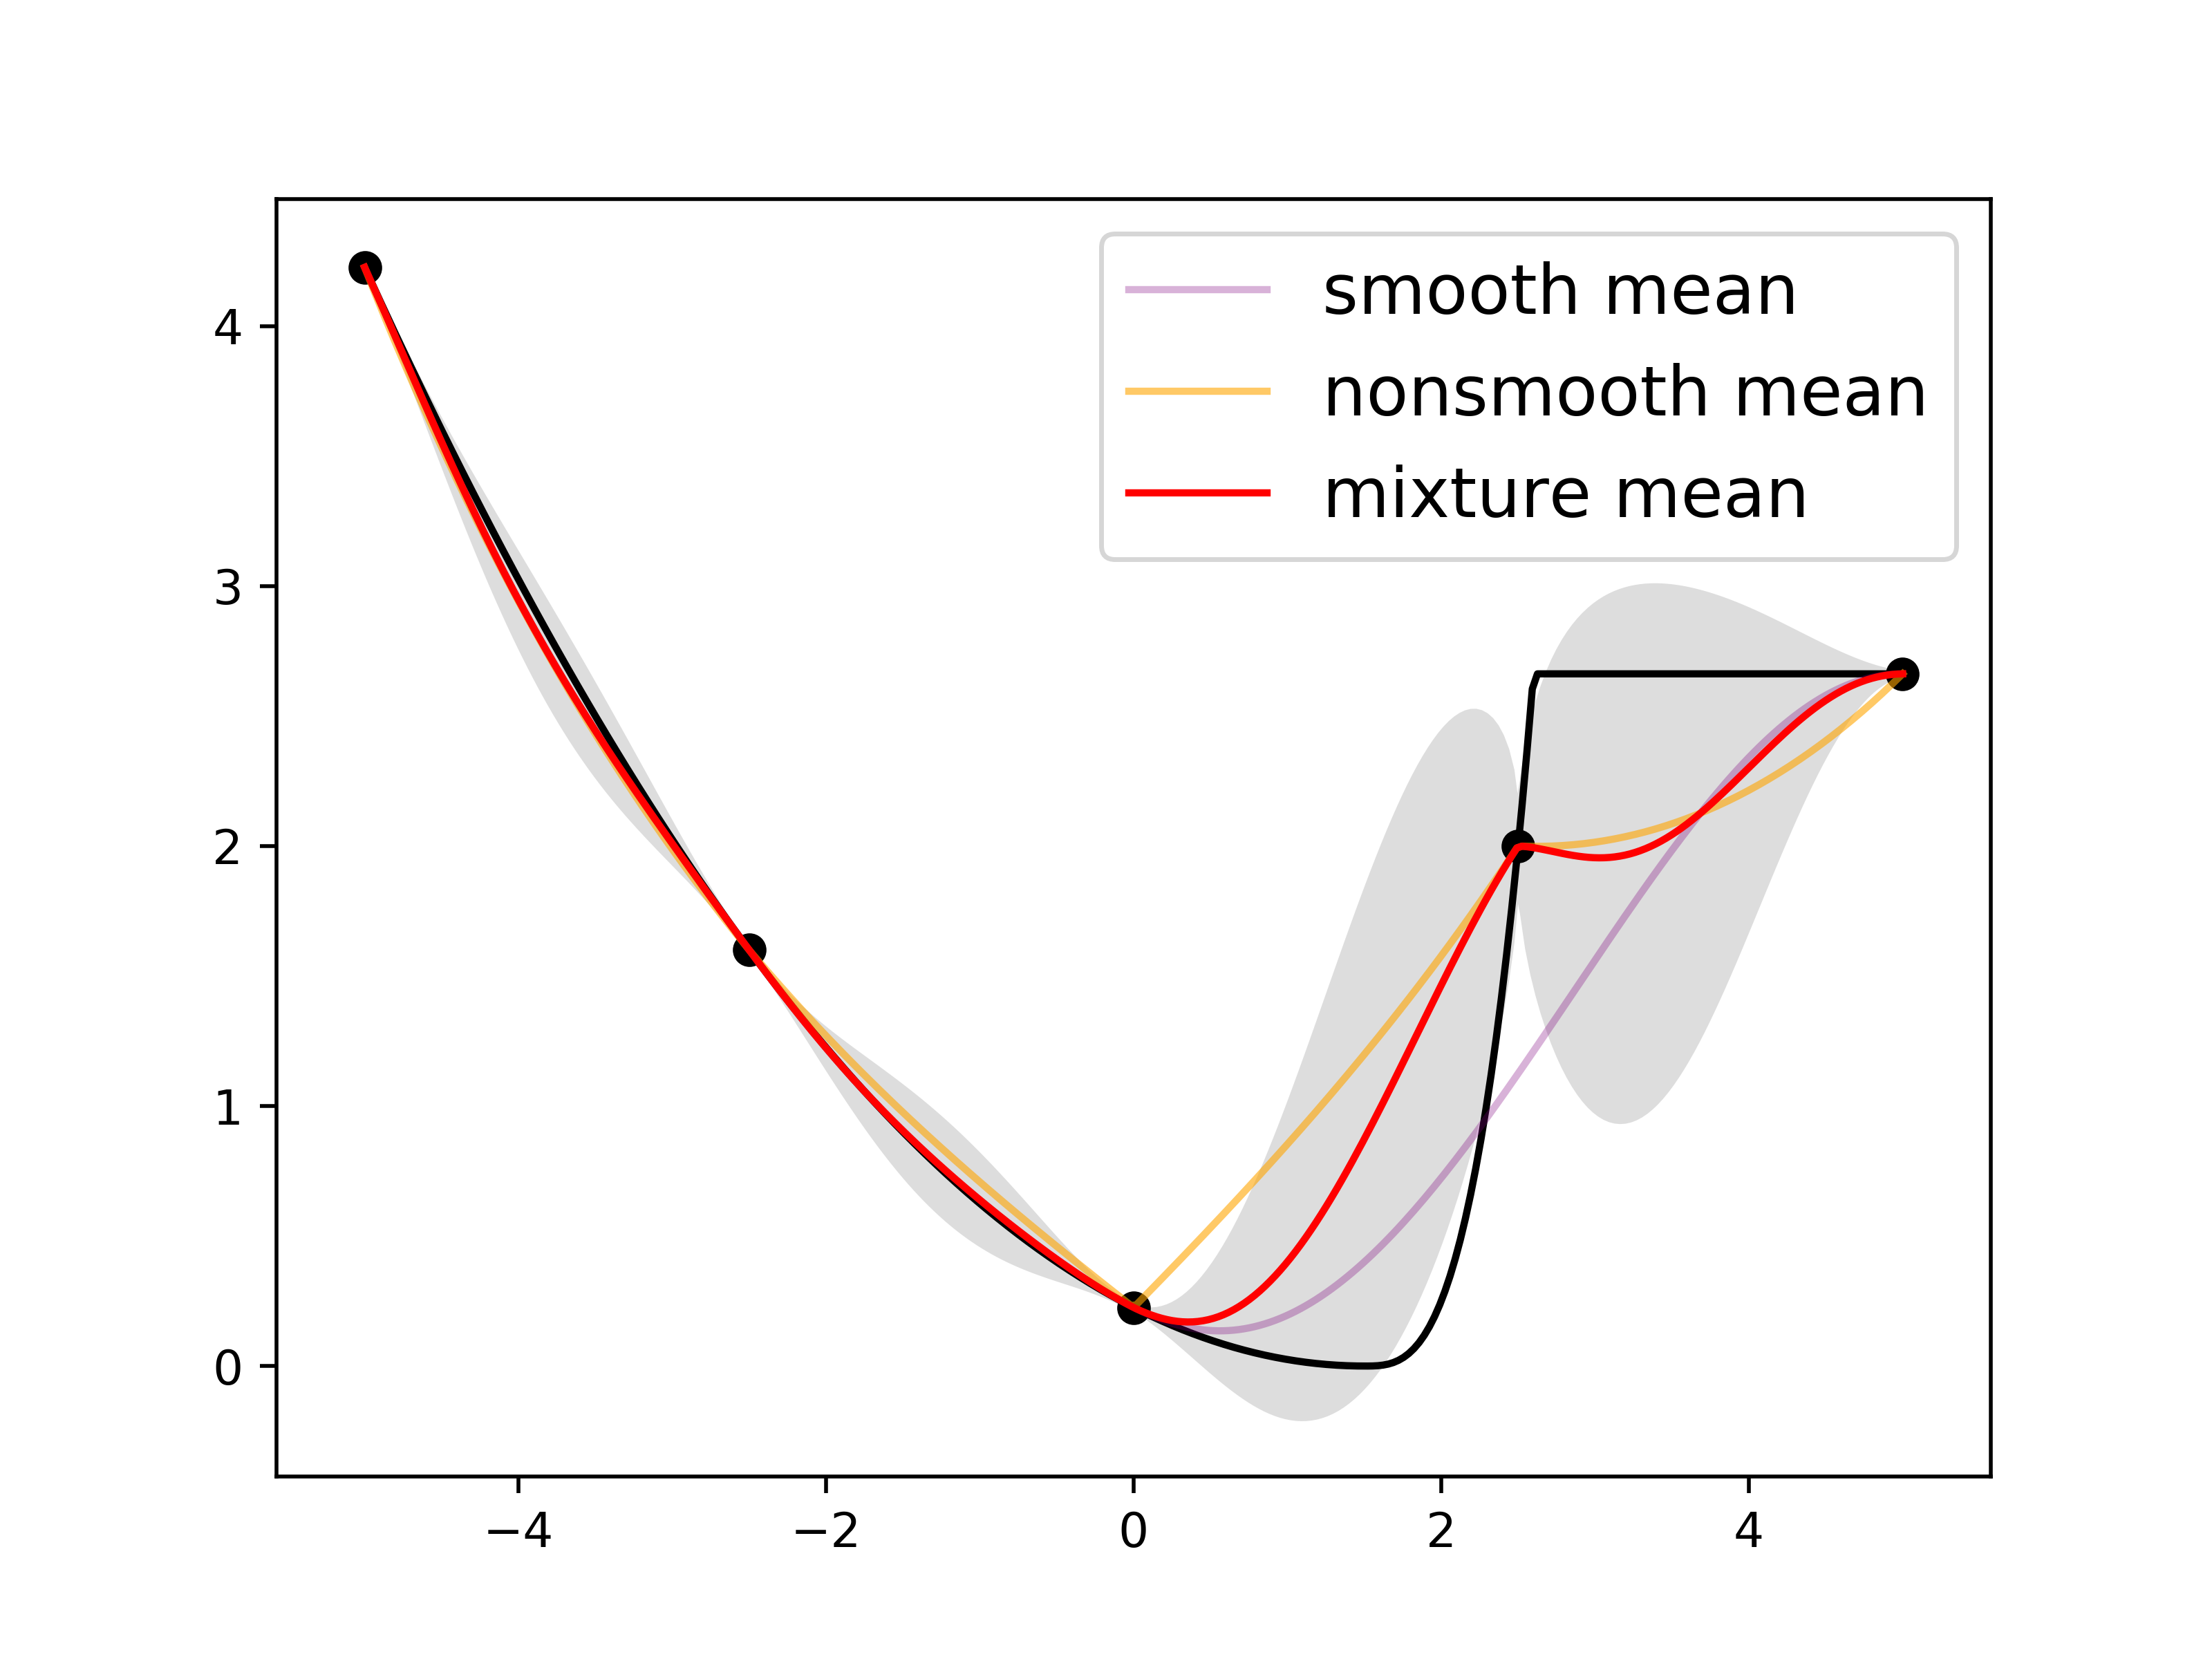
\includegraphics[scale=0.35]{figures/kink-mixture.png}
      \caption{\textbf{Mixture of GPs}}
    \end{subfigure}
    \begin{subfigure}[b]{.4\textwidth}
      \centering
      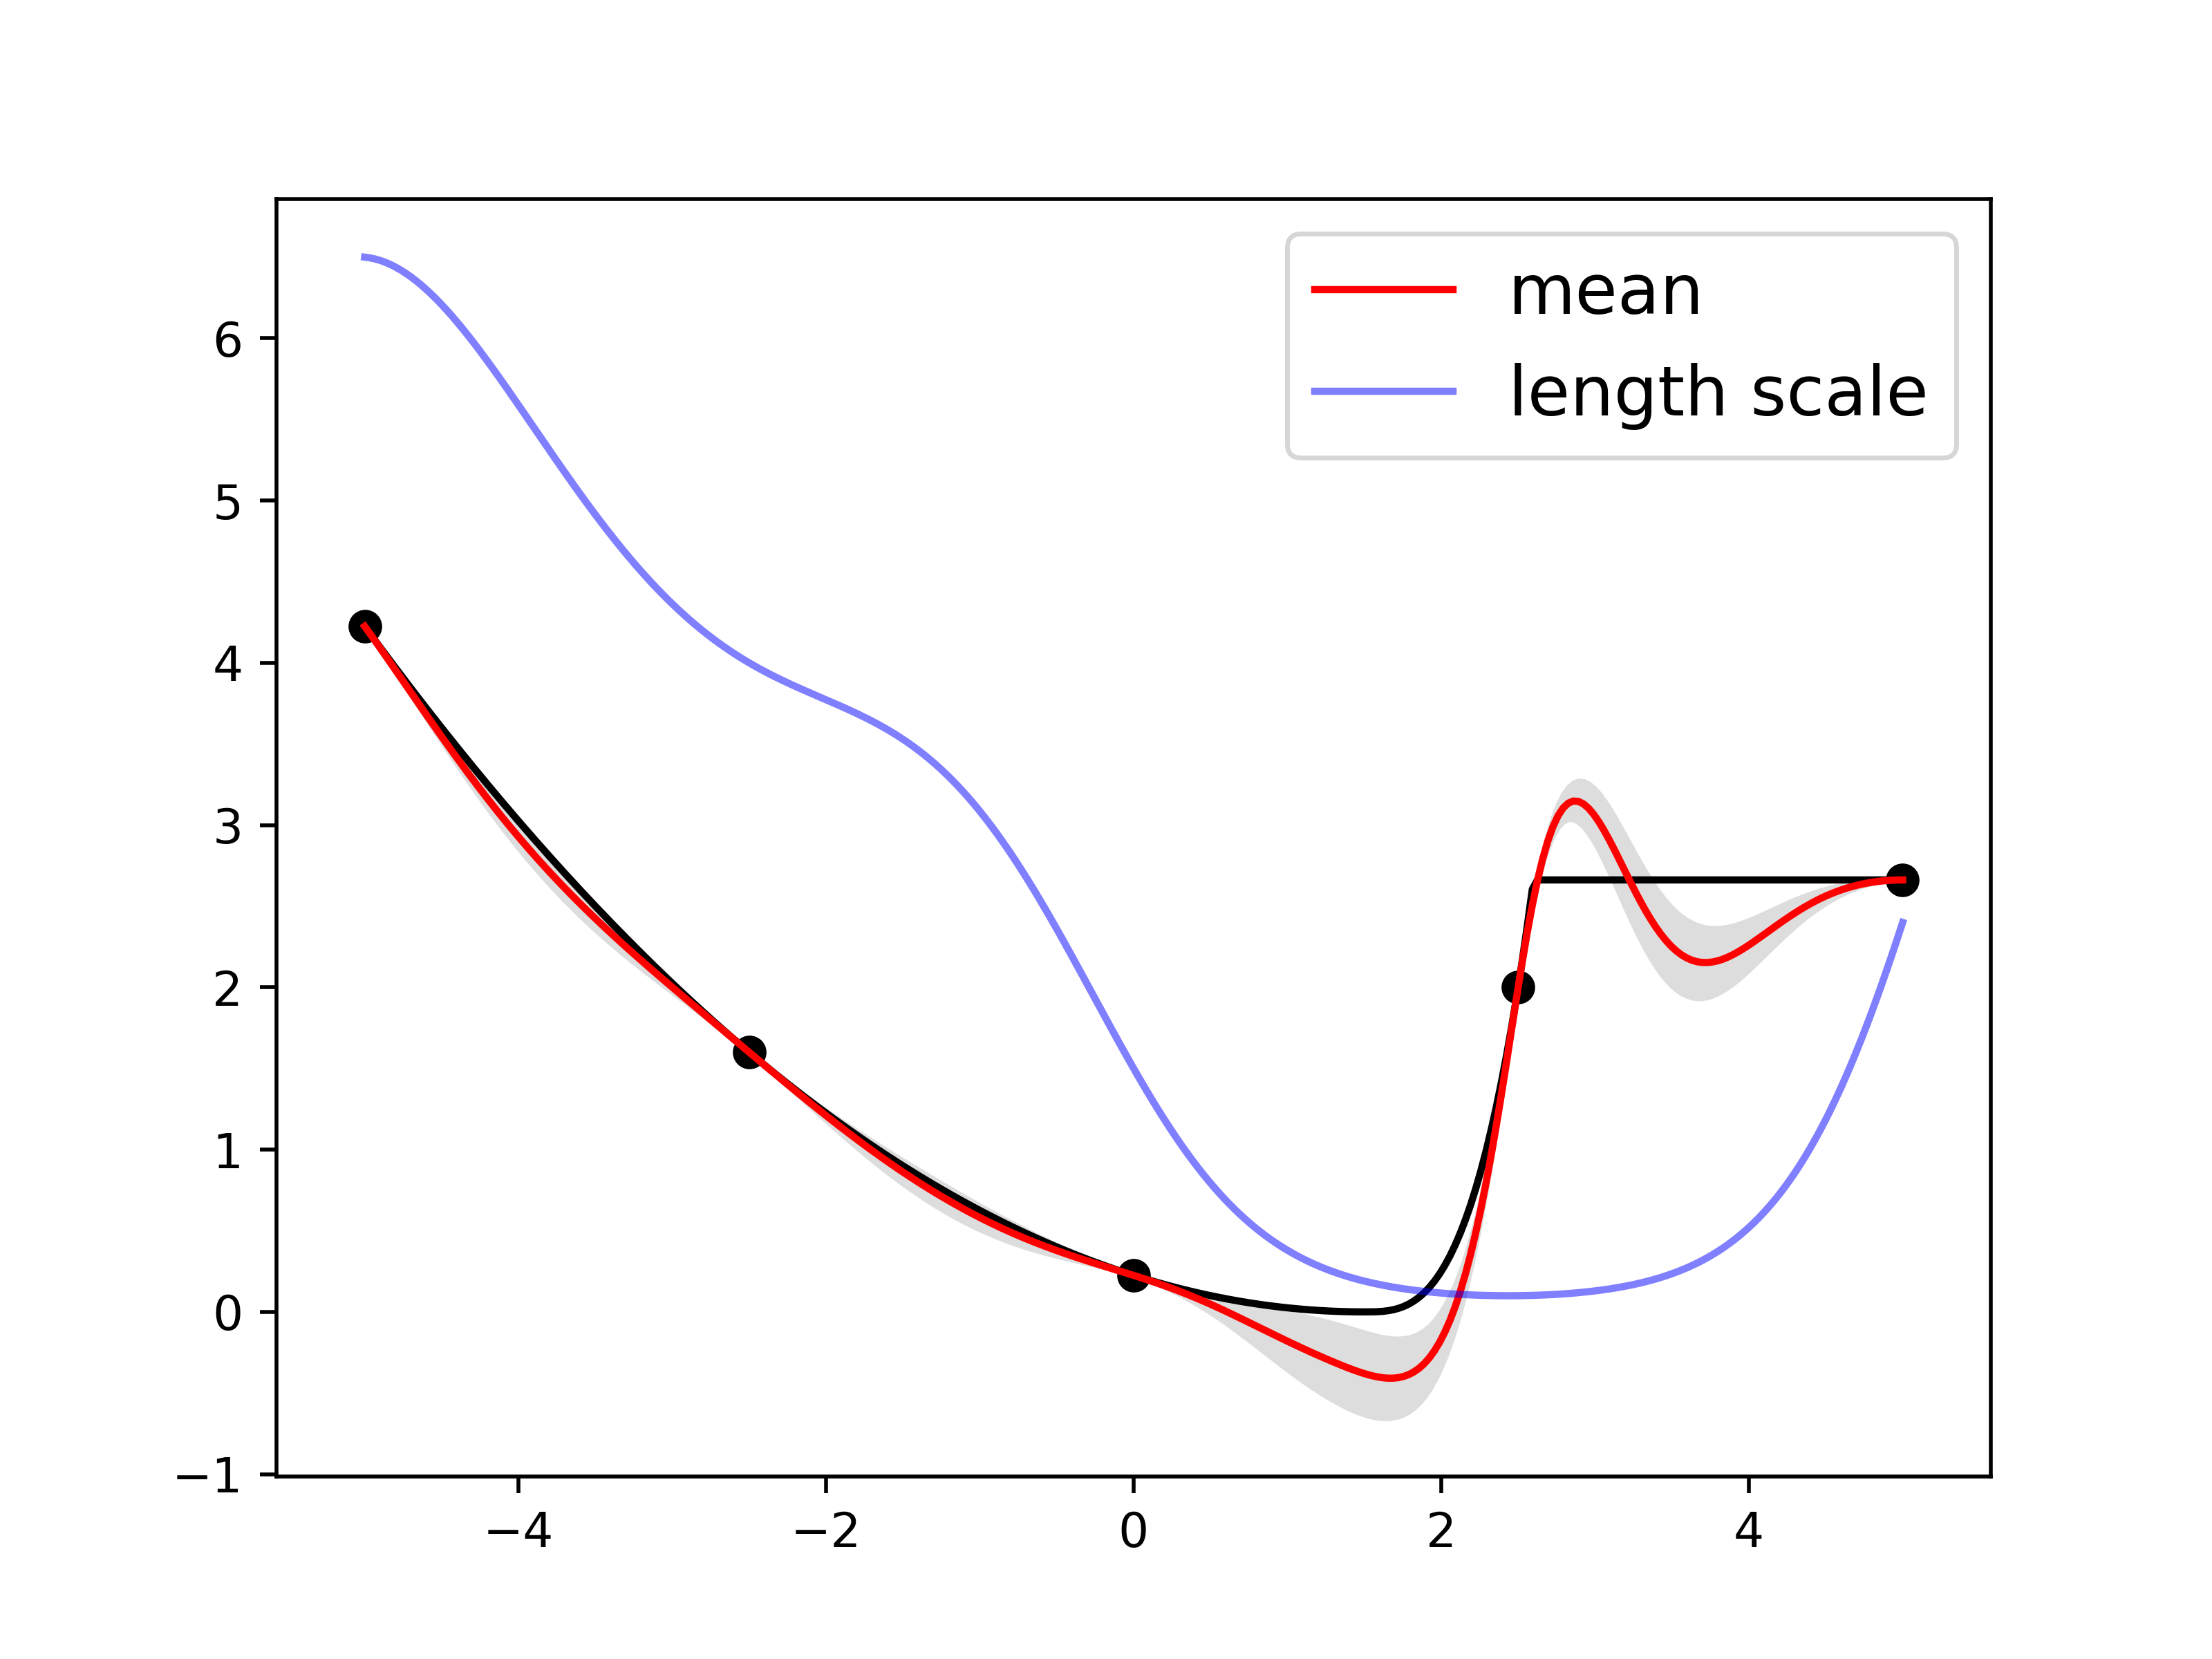
\includegraphics[scale=0.35]{figures/kink-length.png}
      \caption{\textbf{Nonstationary length scale}}
    \end{subfigure}%
    \begin{subfigure}[b]{.4\textwidth}
      \centering
      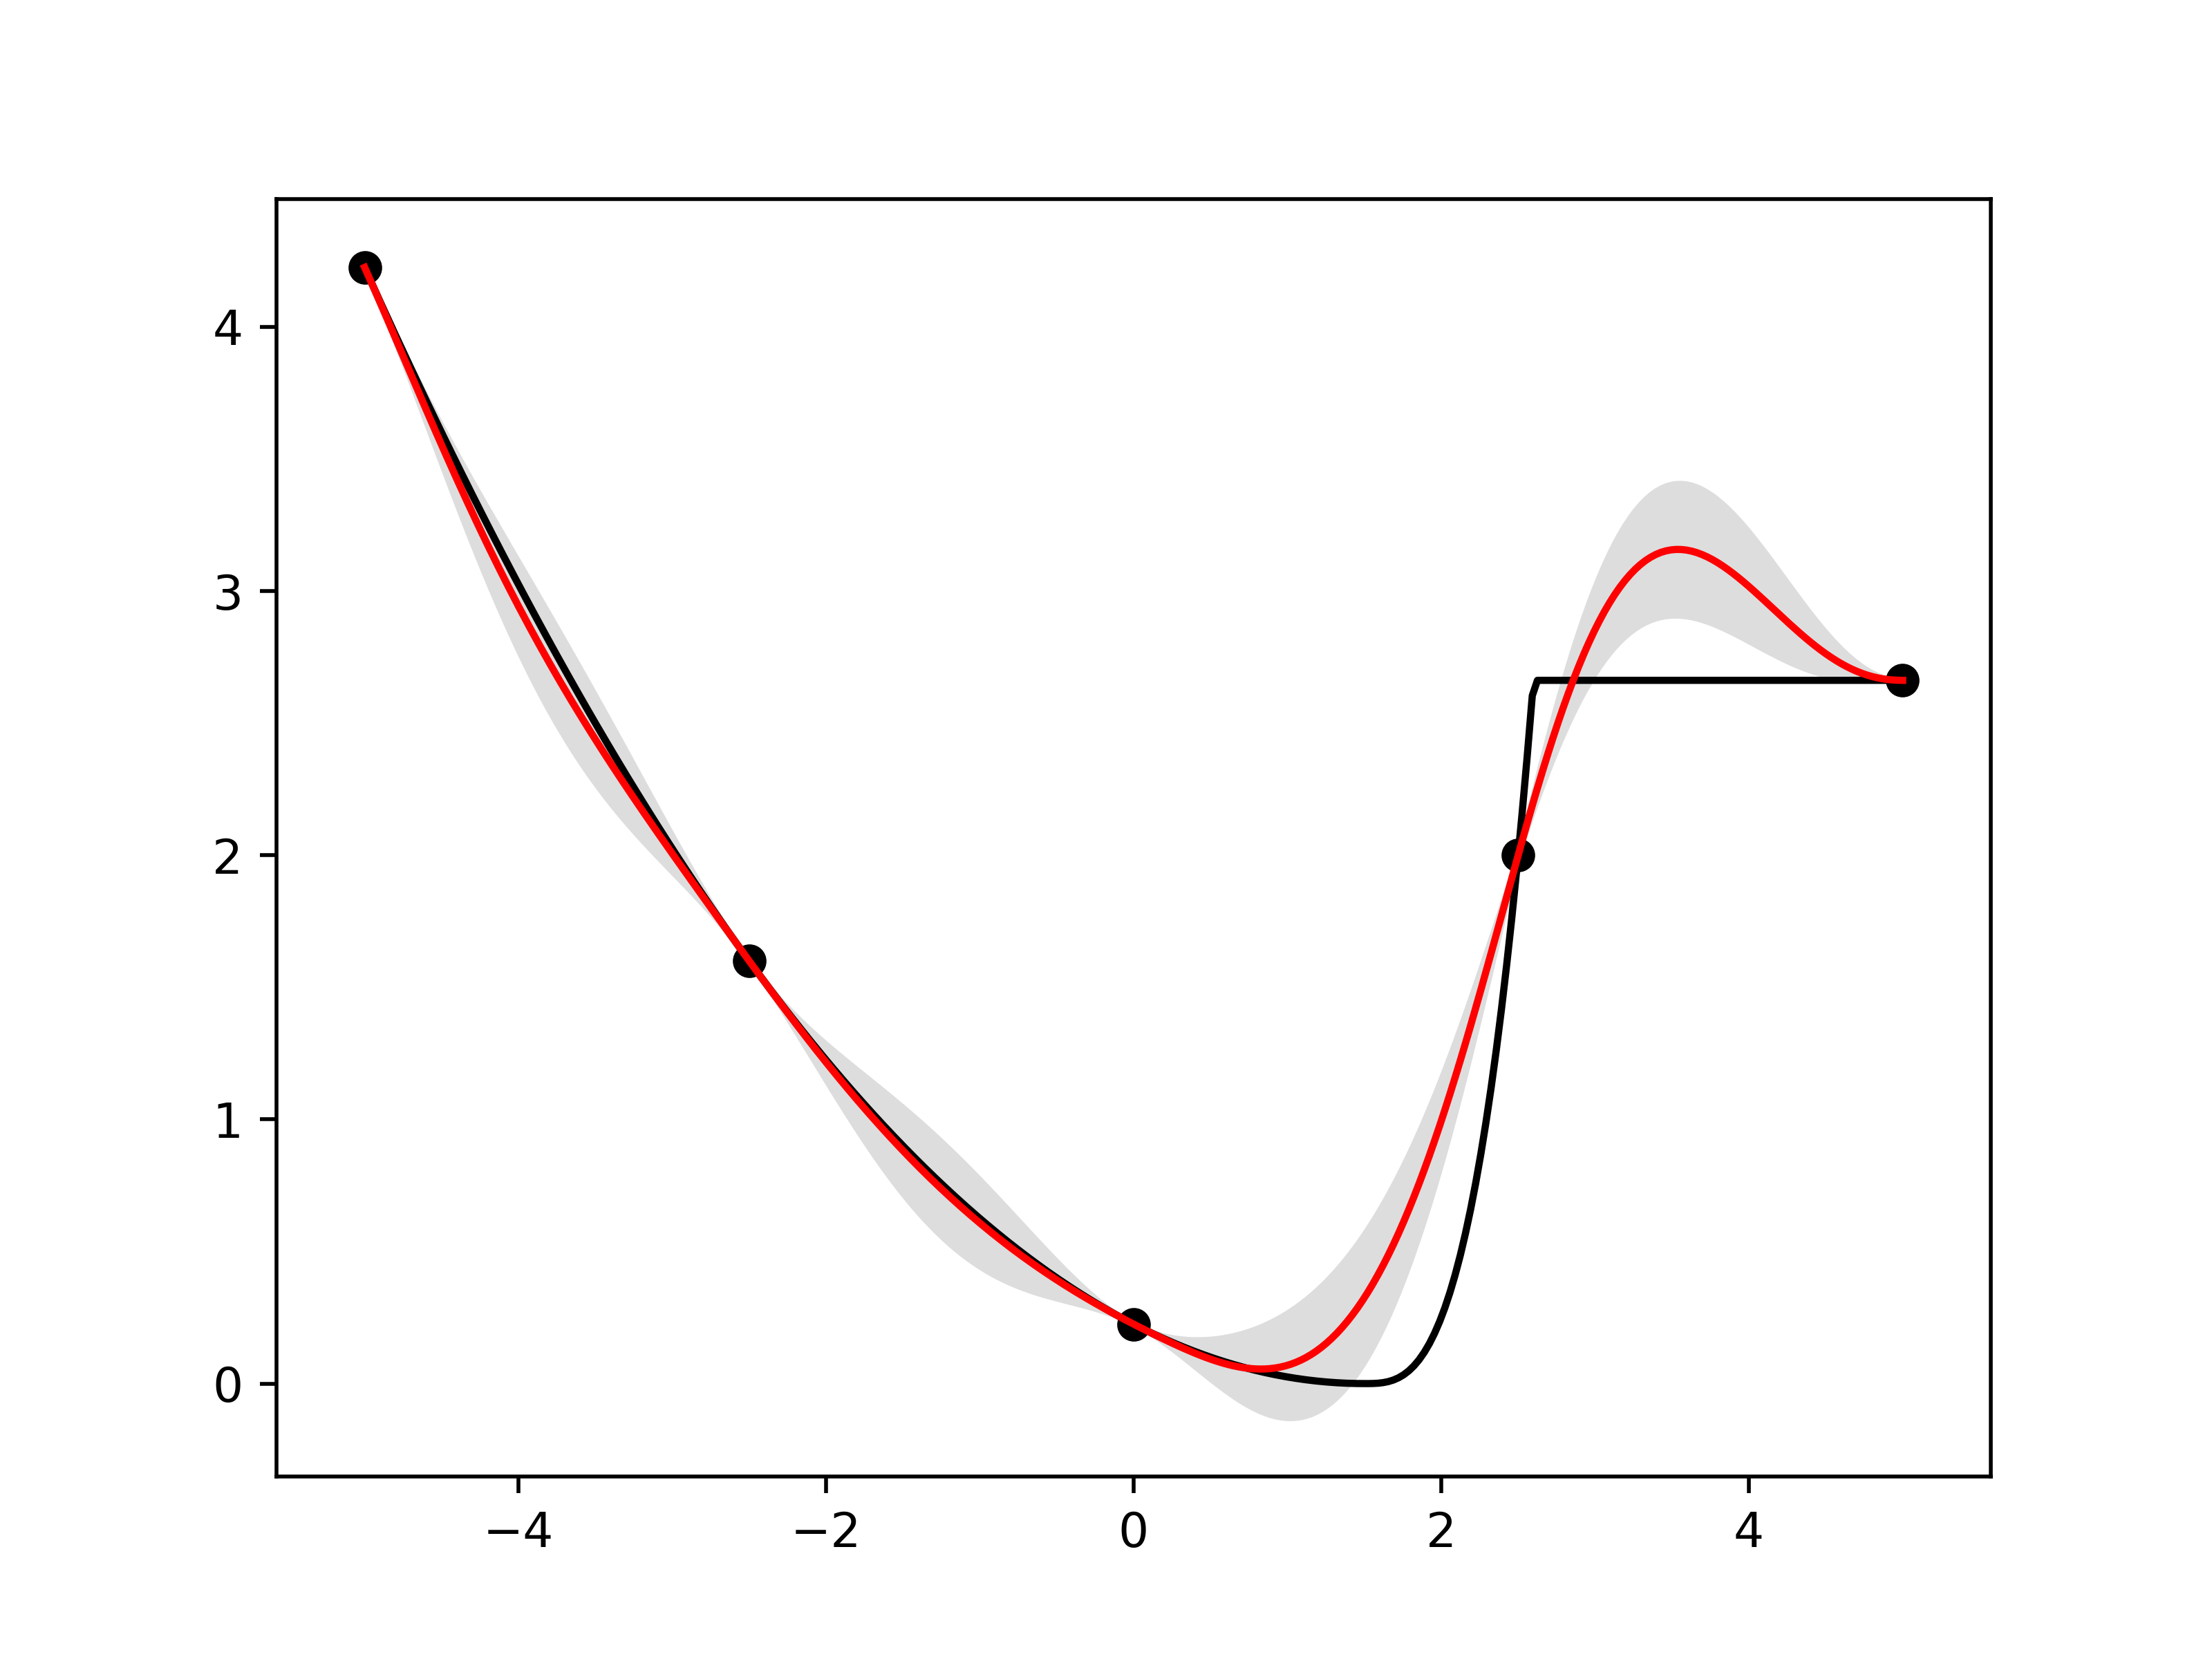
\includegraphics[scale=0.35]{figures/kink-noisy.png}
      \caption{\textbf{Additive derivative noise}}
    \end{subfigure}
		\caption{Gaussian process approximations to a piecewise analytic function using five regularly spaced inputs with Mat\'ern kernel $\nu = 5/2$. The mean $\hat{b}(\vec{x})$ of the length scale GP is shown in blue.}
		\label{nonstationary}
\end{figure}

\section{Results}
We now present performance results for the posterior distribution of each process described above as an approximation to low-dimensional piecewise analytic functions. For a visual comparison see Figure~\ref{nonstationary}, which shows each of the four methods applied to the same piecewise analytic function used in Figure~\ref{kink}. We continue by studying both the numerical error of the posterior mean and how well the posterior variance matches this error.

\subsection{Posterior mean error}
We first test the performance of the methods just described by studying the integrated squared error
$$ ISE(\hat{f}) = \int_\Omega \Big(f(\vec{x})- \hat{f}(\vec{x})\Big)^2 d\vec{x}, $$
where $f$ is the true function and $\hat{f}$ is the posterior mean of the Gaussian process. We numerically approximate the above integral using the adaptive quadrature algorithm by Genz~\cite{genz1991adaptive}, which recursively partitions the domain and applies a quadrature rule to each subdomain until an error estimate tolerance is met, making it suitable to the nondifferentiable squared error. We test each approach using regular grid sampling designs with an increasing number of observations.

\begin{figure}
		\centering
		\captionsetup{justification=centering}
    \begin{subfigure}[b]{.5\textwidth}
      \centering
      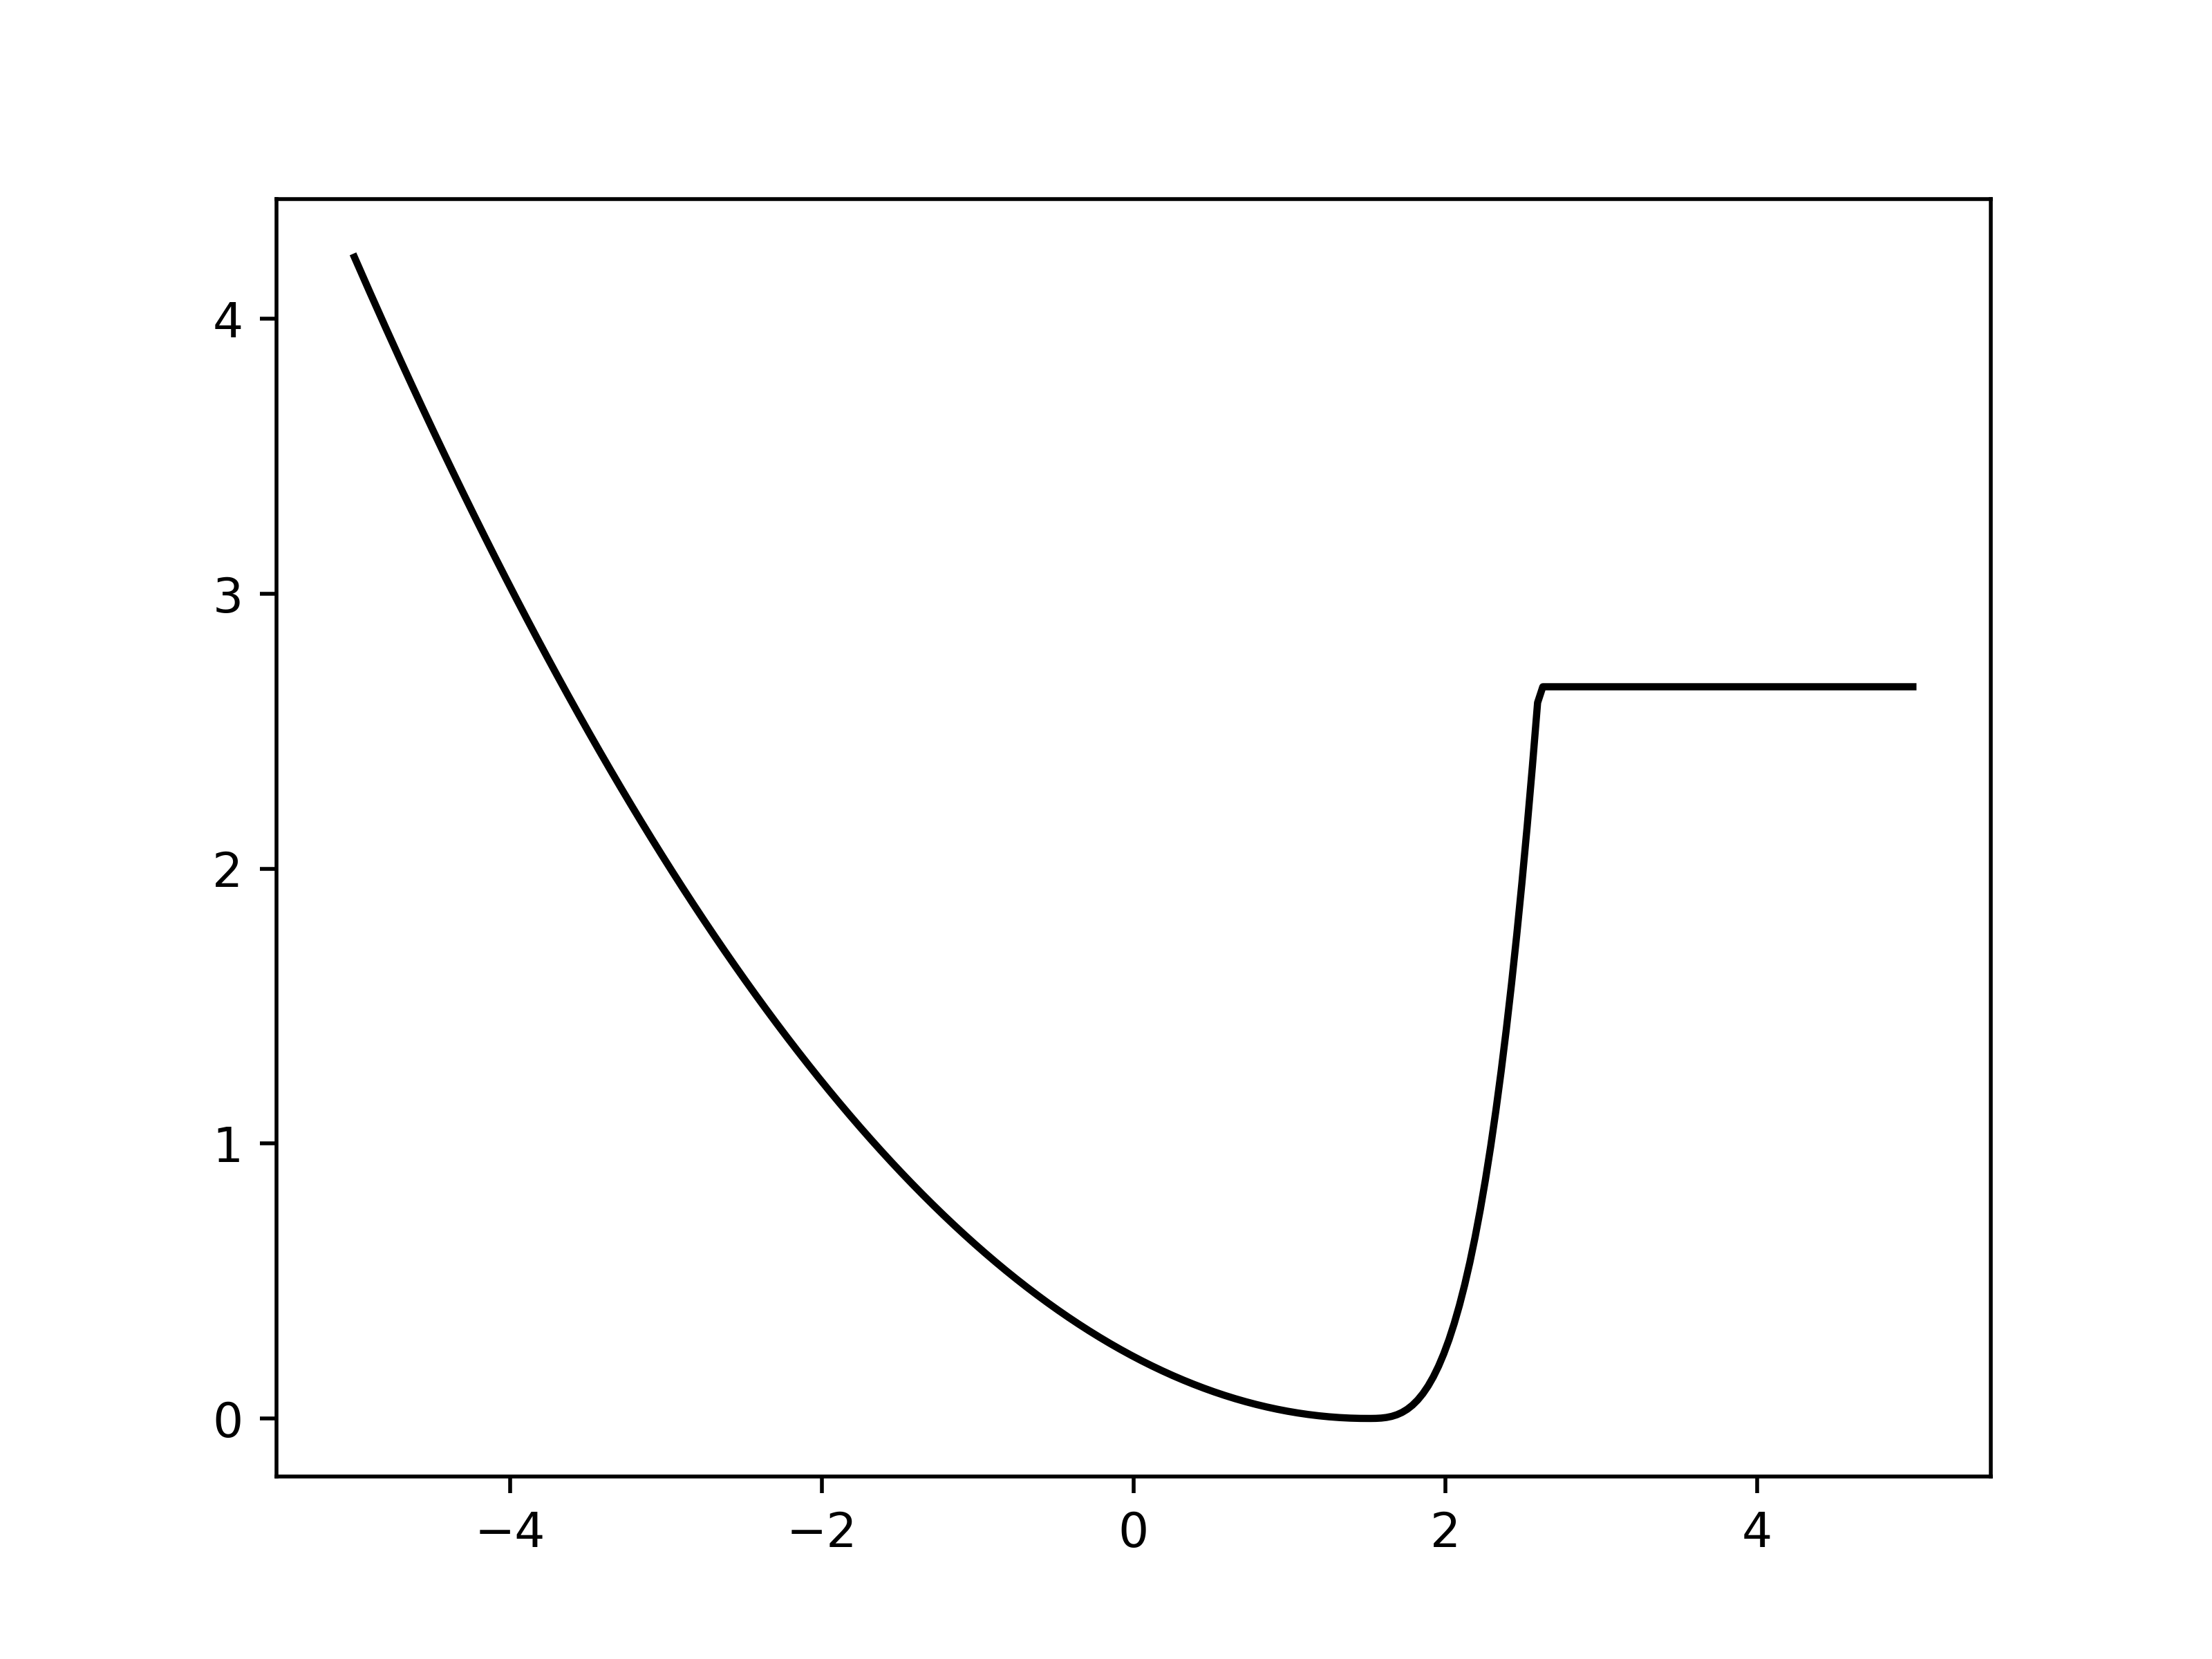
\includegraphics[scale=0.4]{figures/kink.png}
      \caption{\textbf{True function}}
    \end{subfigure}%
    \begin{subfigure}[b]{.5\textwidth}
      \centering
      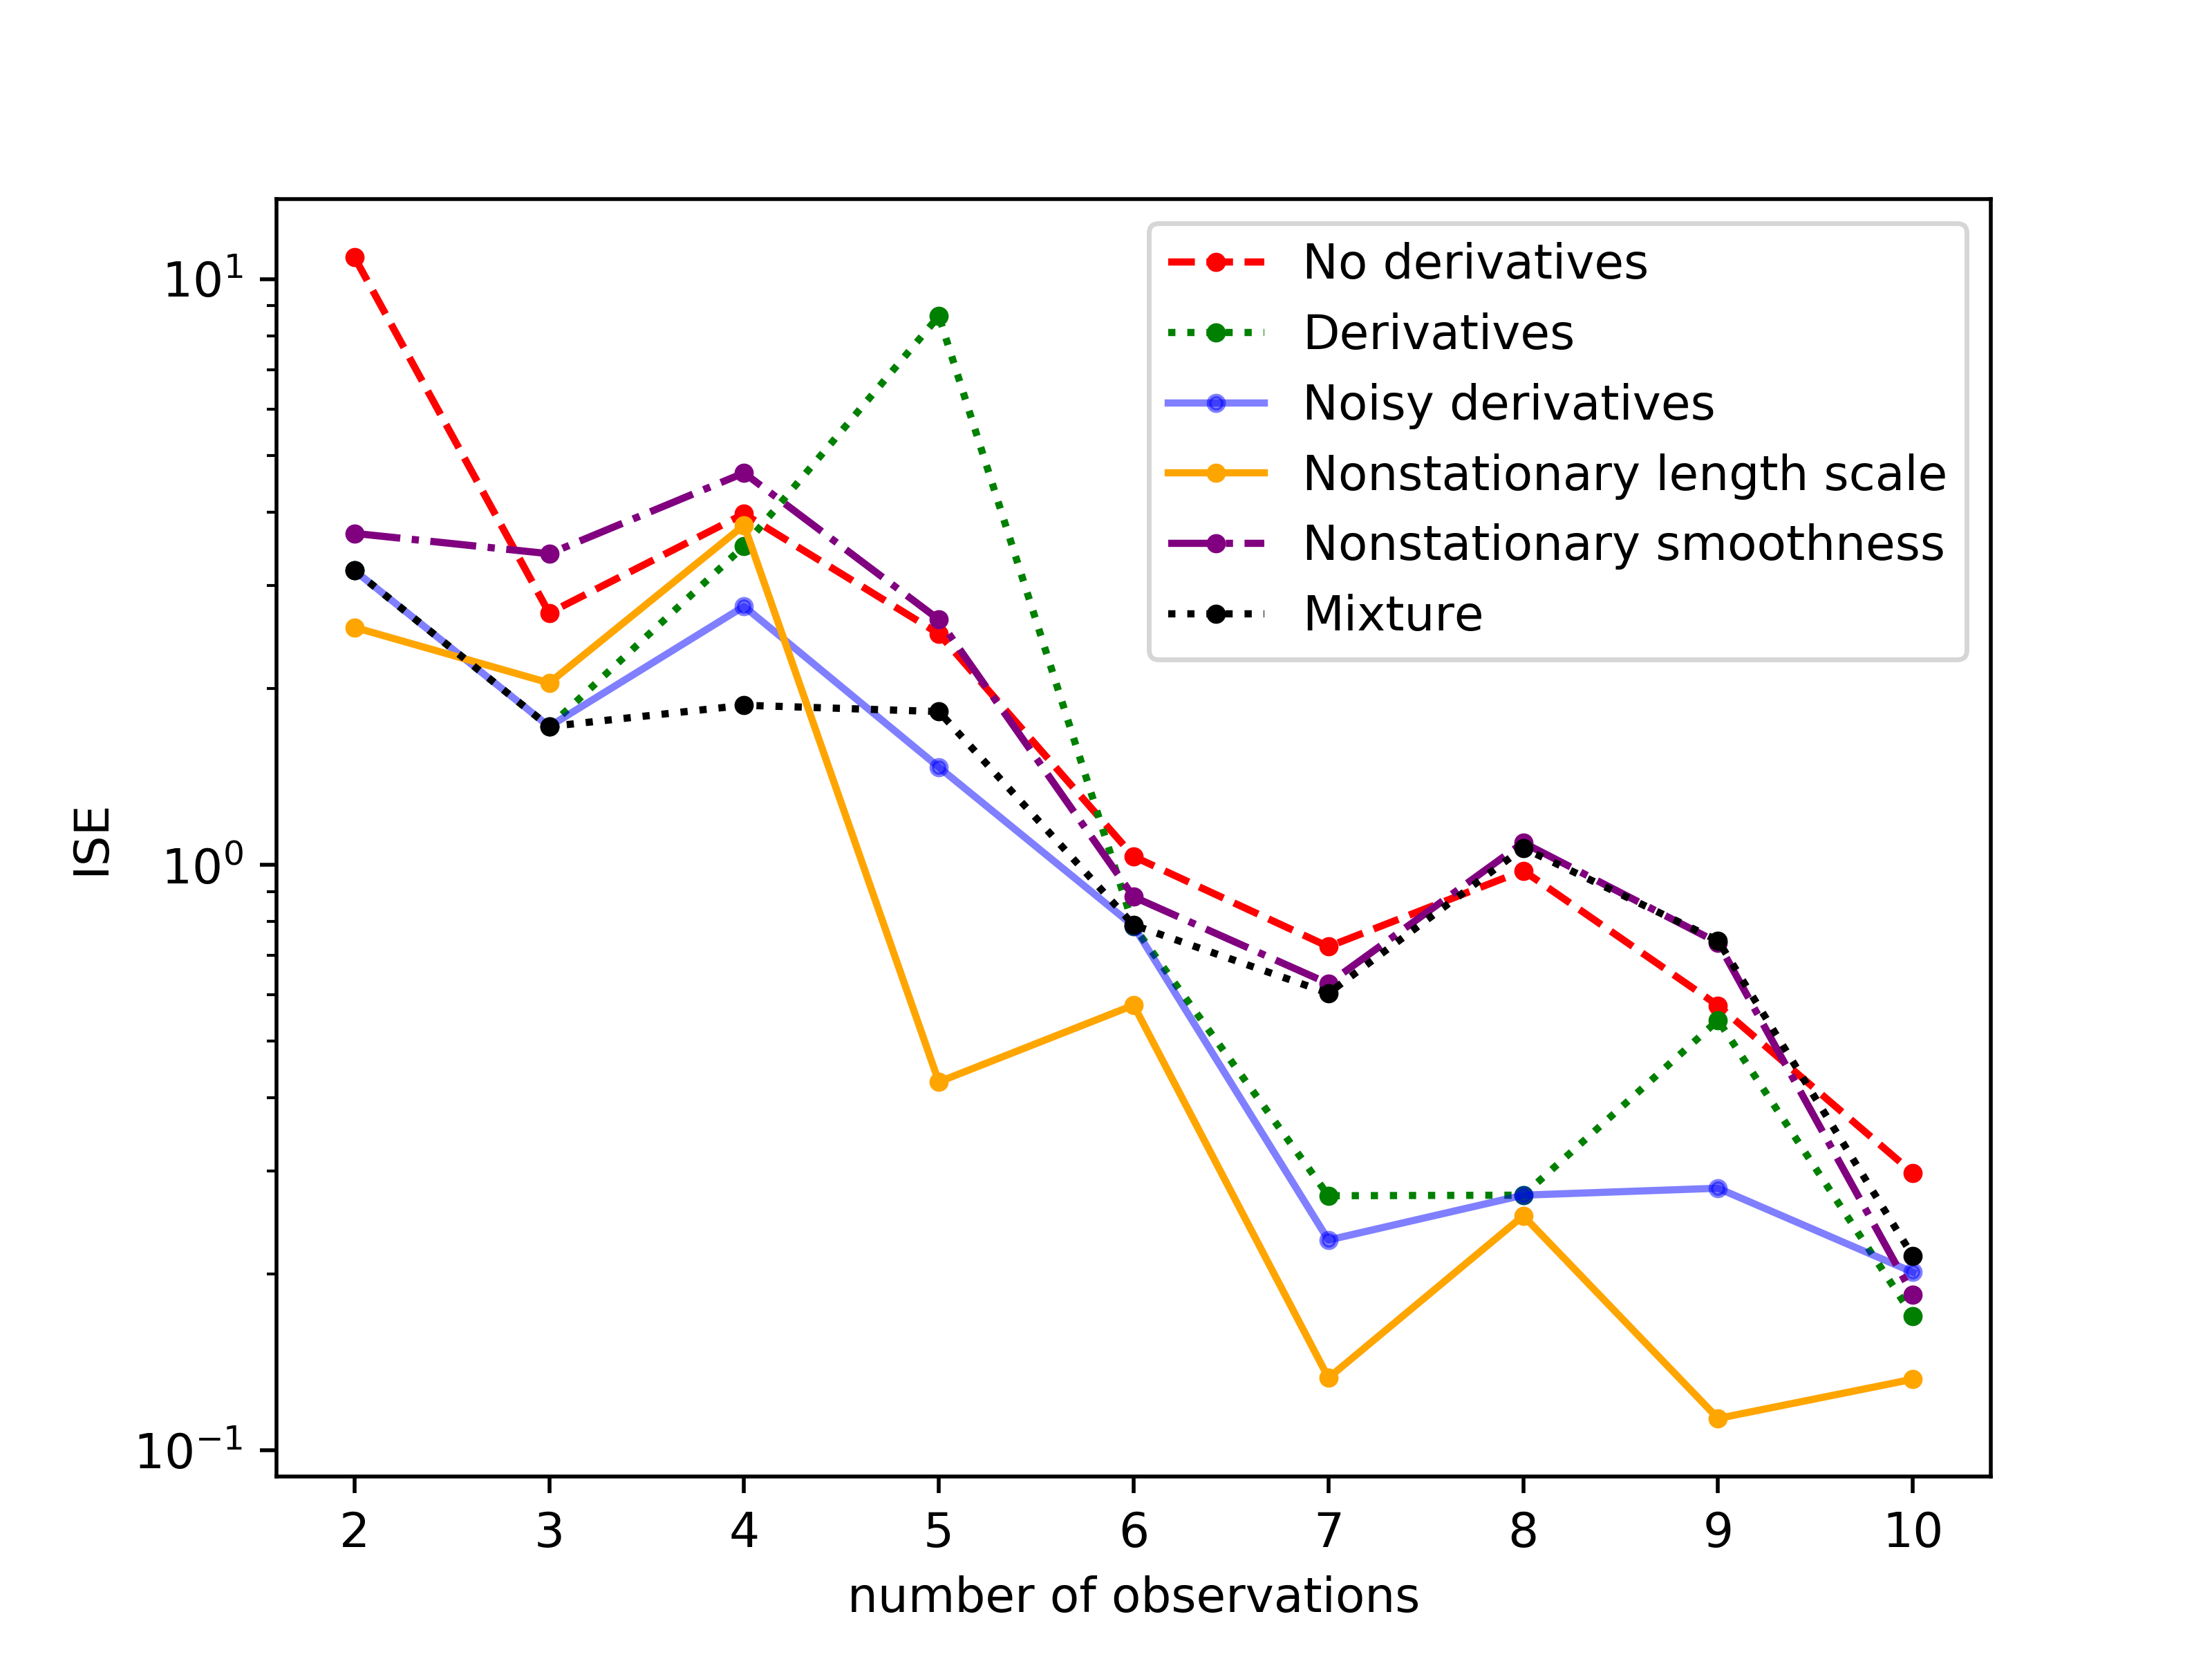
\includegraphics[scale=0.4]{figures/regular-1D-all.png}
      \caption{\textbf{ISE}}
    \end{subfigure}
		\caption{Integrated squared error between the piecewise analytic function $f$ used throughout and the GP posterior mean constructed from observations on regular grids.}
		\label{regular-1D}
\end{figure}

For the one-dimensional test case given by Algorithm~\ref{kink-code} and shown in Figure~\ref{regular-1D}, we find that the nonstationary smoothness method performs similarly to the standard GP. This is to be expected, as neither method uses gradient observations. The mixture approach shows promising performance for low sample densities, but quickly approaches the standard GP in accuracy because the mixture mean near kinks closely resembles that of the standard GP, and thus accumulates large errors in these regions.

In contrast, the additive derivative noise model and the nonstationary length scale method offer improvement over both standard and gradient-interpolating GPs for most sample densities. This is especially apparent in cases where the sample density is relatively low and an observation falls near a branching point. For gradient-interpolating GPs, such cases typically cause oscillations in the posterior mean, as seen in Figure~\ref{regular-1D} when $n$=5 or 9. In these cases, the noise free gradient-interpolating GP performs comparably to or worse than the standard GP. Oscillations are significantly reduced by both additive derivative noise and nonstationary length scale methods in these cases, leading to lower posterior mean error.

\begin{figure}[H]
		\centering
		\captionsetup{justification=centering}
    \begin{subfigure}[t]{.33\textwidth}
      \centering
      \includegraphics[scale=0.4]{figures/f-2D.eps}
      \caption{\textbf{True function in $\R^2$}}
    \end{subfigure}%
    \begin{subfigure}[t]{.33\textwidth}
      \centering
      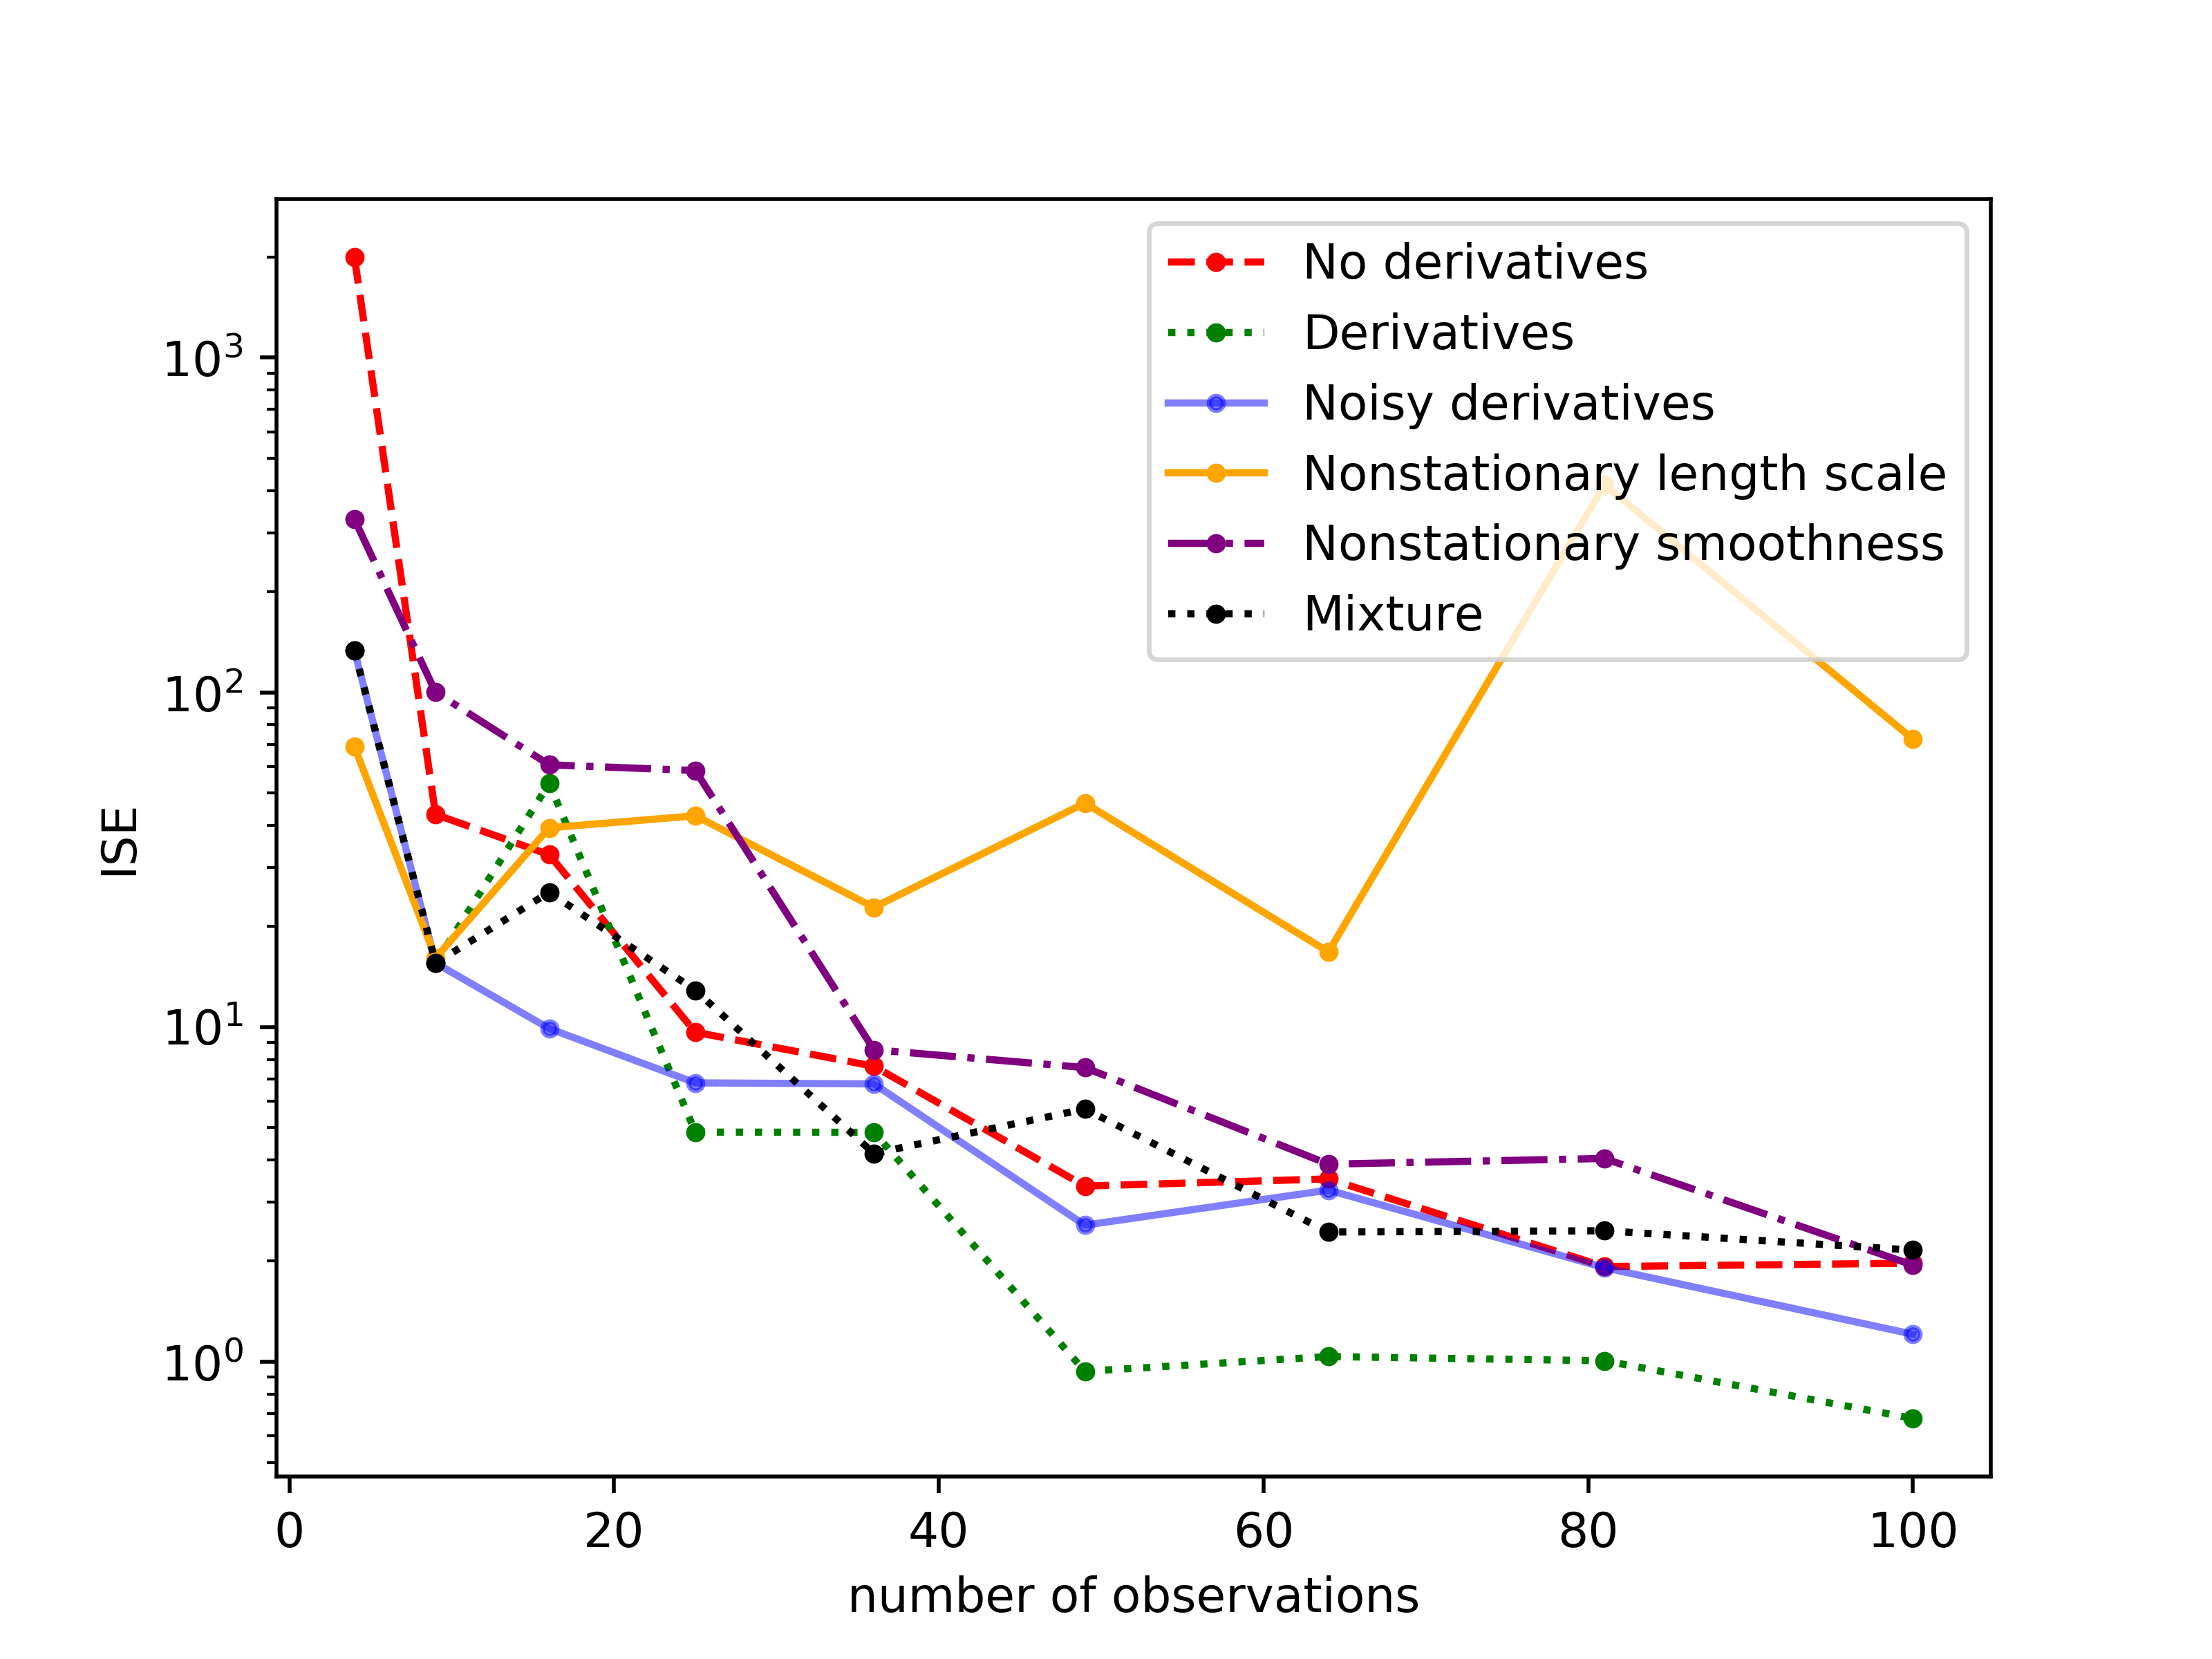
\includegraphics[scale=0.38]{figures/regular-2D-new.png}
      \caption{\textbf{ISE in $\R^2$}}
    \end{subfigure}
    \begin{subfigure}[t]{.33\textwidth}
      \centering
      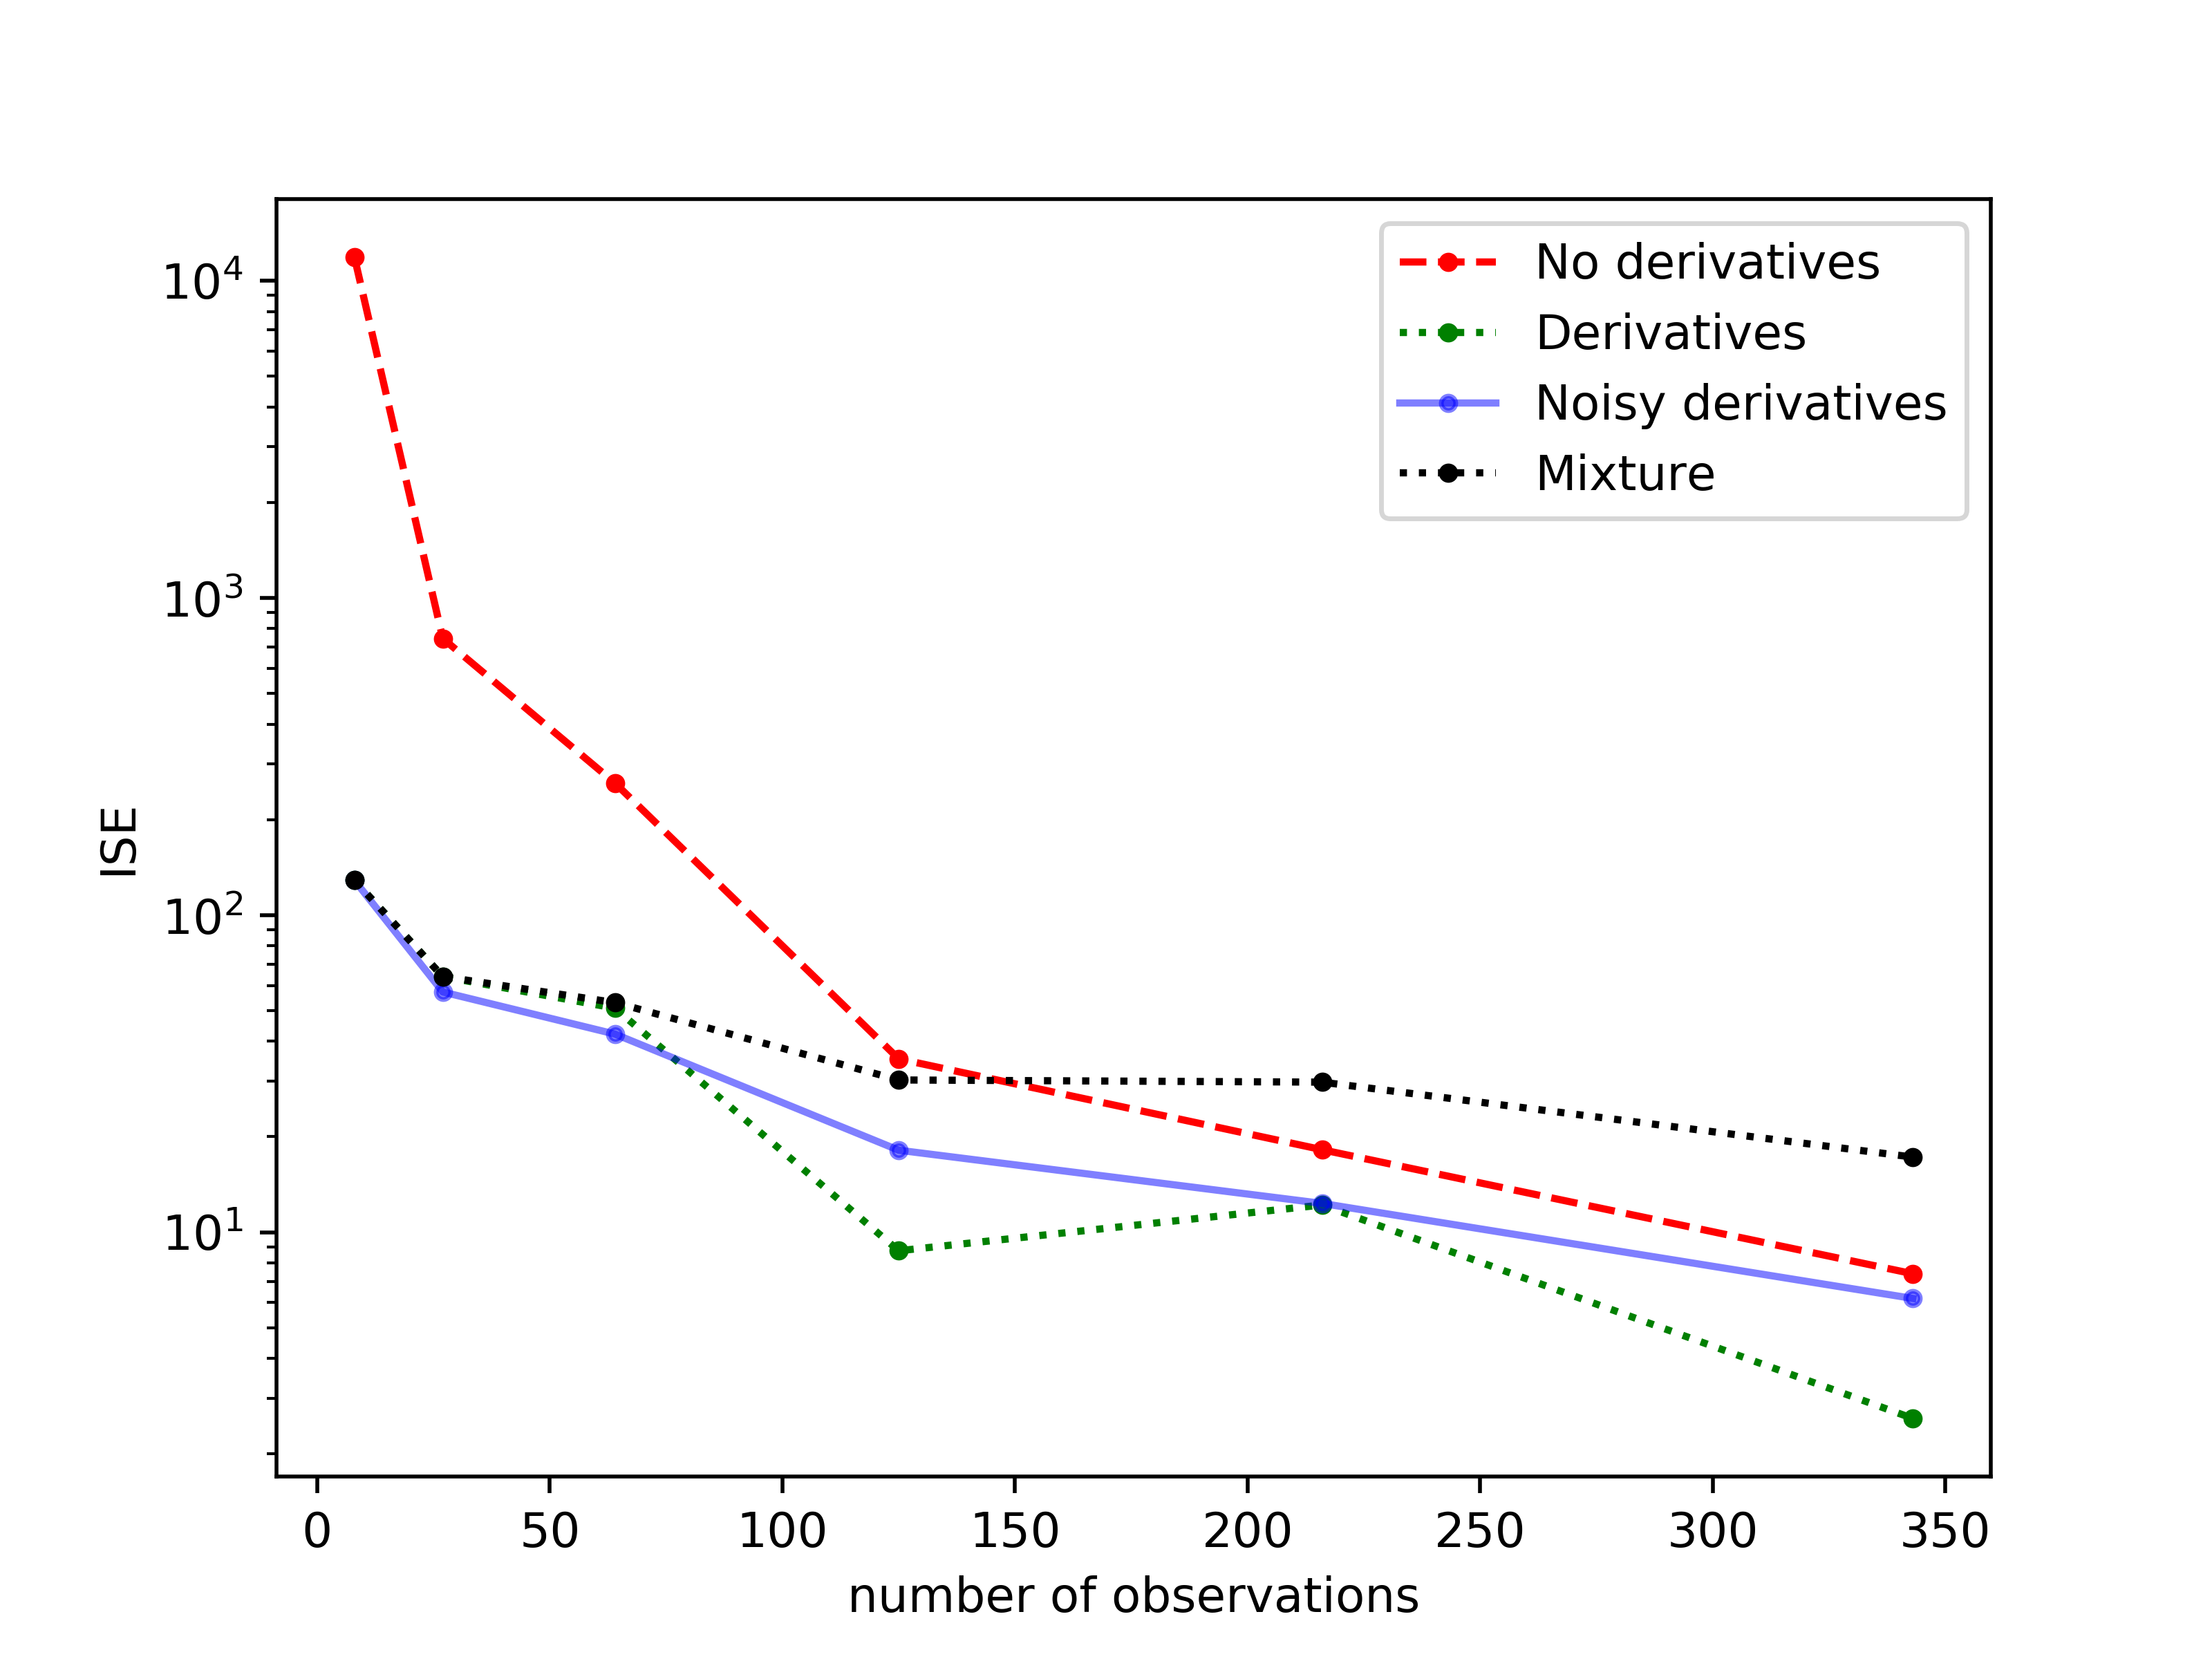
\includegraphics[scale=0.38]{figures/regular-3D-new.png}
      \caption{\textbf{ISE in $\R^3$}}
    \end{subfigure}
		\caption{Integrated squared error between \texttt{rad1} and the GP posterior mean. Gaussian processes constructed from observations on regular grids.}
		\label{regular-2D}
\end{figure}
\begin{algorithm}[H]
    \captionsetup{justification=centering}
    \begin{algorithmic}
    \IF{$g_1(\vec{x}) \geq 0$}
        \RETURN $\norm{\vec{x}}_2^2 - 4$
    \ELSIF{$g_2(\vec{x}) \geq 0$}
        \RETURN $-2\norm{\vec{x}}_2^2 + 2$
    \ELSE
        \RETURN $3\norm{\vec{x}}_2^2 - 3$
    \ENDIF
    \end{algorithmic}
    \caption{: \texttt{rad1}$(\vec{x})$ : $g_1(\vec{x}) = \norm{\vec{x}}_2^2 - 2$, $g_2(\vec{x}) = \norm{\vec{x}}_2^2 - 1$}
	\label{radial-code}
\end{algorithm}

For testing in higher dimensions, we use two piecewise analytic radial functions \texttt{rad1} and \texttt{rad2}. The first, \texttt{rad1}, is given by Algorithm~\ref{radial-code} with nondifferentiabilities on the $(p-1)$-spheres $\norm{\vec{x}}_2^2 = 1$ and $\norm{\vec{x}}_2^2 = 2$ in $\R^p$. The nonstationary smoothness and nonstationary length scale methods are prohibitively expensive with our current computational methods for more than a hundred or so samples in three dimensions due to the cost of computing the posterior mean for each directional branching distance GP at every evaluation of the kernel function. Therefore we test these methods only in $\R$ and $\R^2$.
We find that in $\R^2$ our additive derivative noise approach is robust to hyperparameter selection and demonstrates significant improvement over both function-interpolating and gradient-interpolating GPs for some low sample densities where the gradient-interpolating GP experiences oscillations, as seen in Figure~\ref{regular-2D} when $n=16$. This improvement is negligible in $\R^3$.

Our other methods do not perform as well as the standard GP in most cases. Although our nonstationary length scale approach produces exceptionally accurate posterior means for most sample densities on our one-dimensional test function, this method is very sensitive to hyperparameter selection, and we observe large errors for many sample densities on both \texttt{rad1} and \texttt{rad2} in $\R^2$. Determining methods of consistent hyperparameter estimation remains the focus of future work, as discussed in Section~\ref{future-work}. Gradient interpolation produces the smallest errors for all sufficiently large sample densities in both $\R^2$ and $\R^3$, indicating that oscillations in \texttt{rad1} are effectively reduced by further sampling, especially in higher dimensions. We now study a second radial function which exhibits persistent oscillation in the posterior mean even for higher sample densities.

Our second radial function is given by
$$\texttt{rad2}(\vec{x}) = \abs{\sin\Big(10e^{-\norm{\vec{x}}_2^2}\Big) + 0.5} - 0.2\norm{\vec{x}}_2^2 + 10.$$
The absolute value can be easily rewritten in our conditional code model using the single branching function $g_1(\vec{x}) = \sin\Big(10e^{-\norm{\vec{x}}_2^2}\Big) + 0.5$. A graph of \texttt{rad2} in $\R$ is given in Figure~\ref{crazy} along with ISE results in $\R$, $\R^2$, and $\R^3$. We see that in this case gradient interpolation causes oscillations in the posterior mean leading to higher errors than the standard GP for a number of sample densities. The nonstationary length scale and nonstationary smoothness methods exhibit unpredictable behavior in both $\R$ and $\R^2$. This is due both to the hyperparameter sensitivity previously discussed as well as the reliance on the branching distance log GPs, which themselves experience oscillation in the center of the input space where the estimated branching distances change rapidly. However, the mixture method and the additive derivative noise method both demonstrate improved accuracy compared to standard and gradient-interpolating GPs for many test cases. Notably, the additive derivative noise model is at least as accurate as the standard GP on all test cases, and is as accurate as the gradient-interpolating GP for low sample densities where it performs well.

These results indicate that adding noise to gradient observations near kinks prevents extreme oscillation due to gradient interpolation, while maintaining increased accuracy compared to function-interpolating GPs for low sample densities. Intuitively, gradients carry significant information about the behavior of the function when few observations are taken, and although exact gradient interpolation can cause oscillation, using gradient information with noise allows us to incorporate the general behavior suggested by gradient observations while avoiding oscillation.

\begin{figure}
		\centering
		\captionsetup{justification=centering}
    \begin{subfigure}[t]{.4\textwidth}
      \centering
      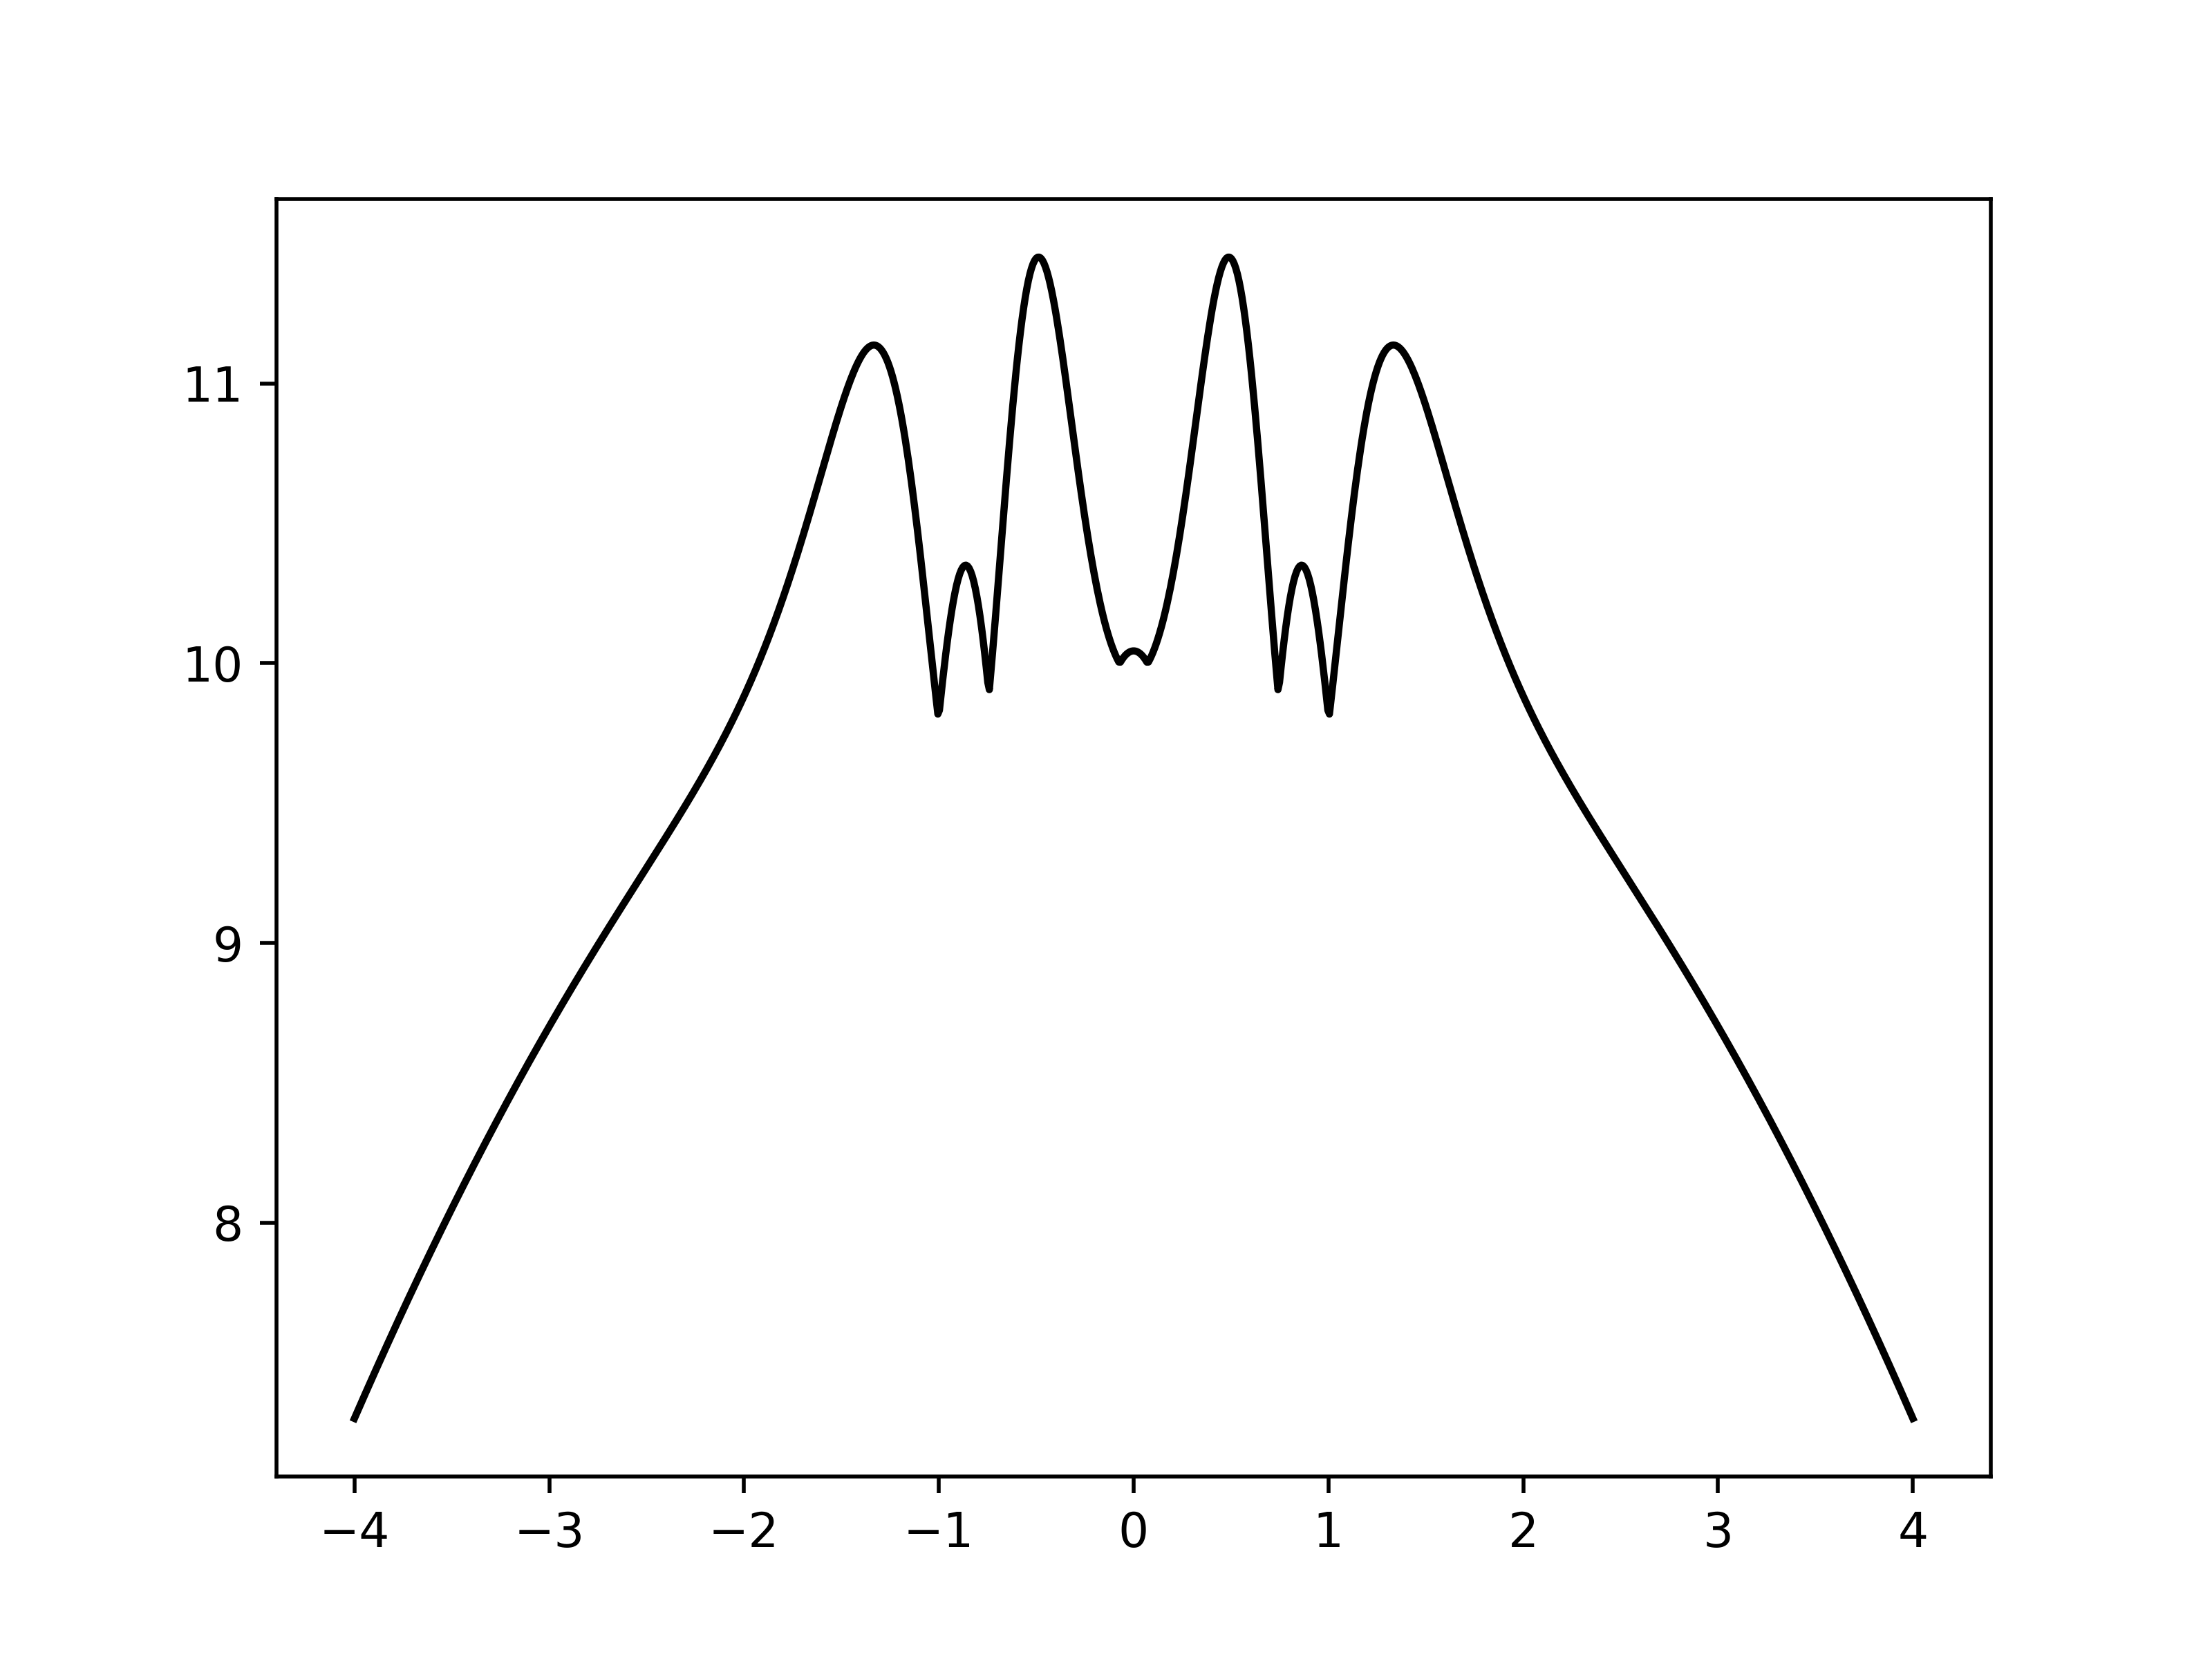
\includegraphics[scale=0.35]{figures/crazy.png}
      \caption{\textbf{True function in $\R$}}
    \end{subfigure}%
    \begin{subfigure}[t]{.4\textwidth}
      \centering
      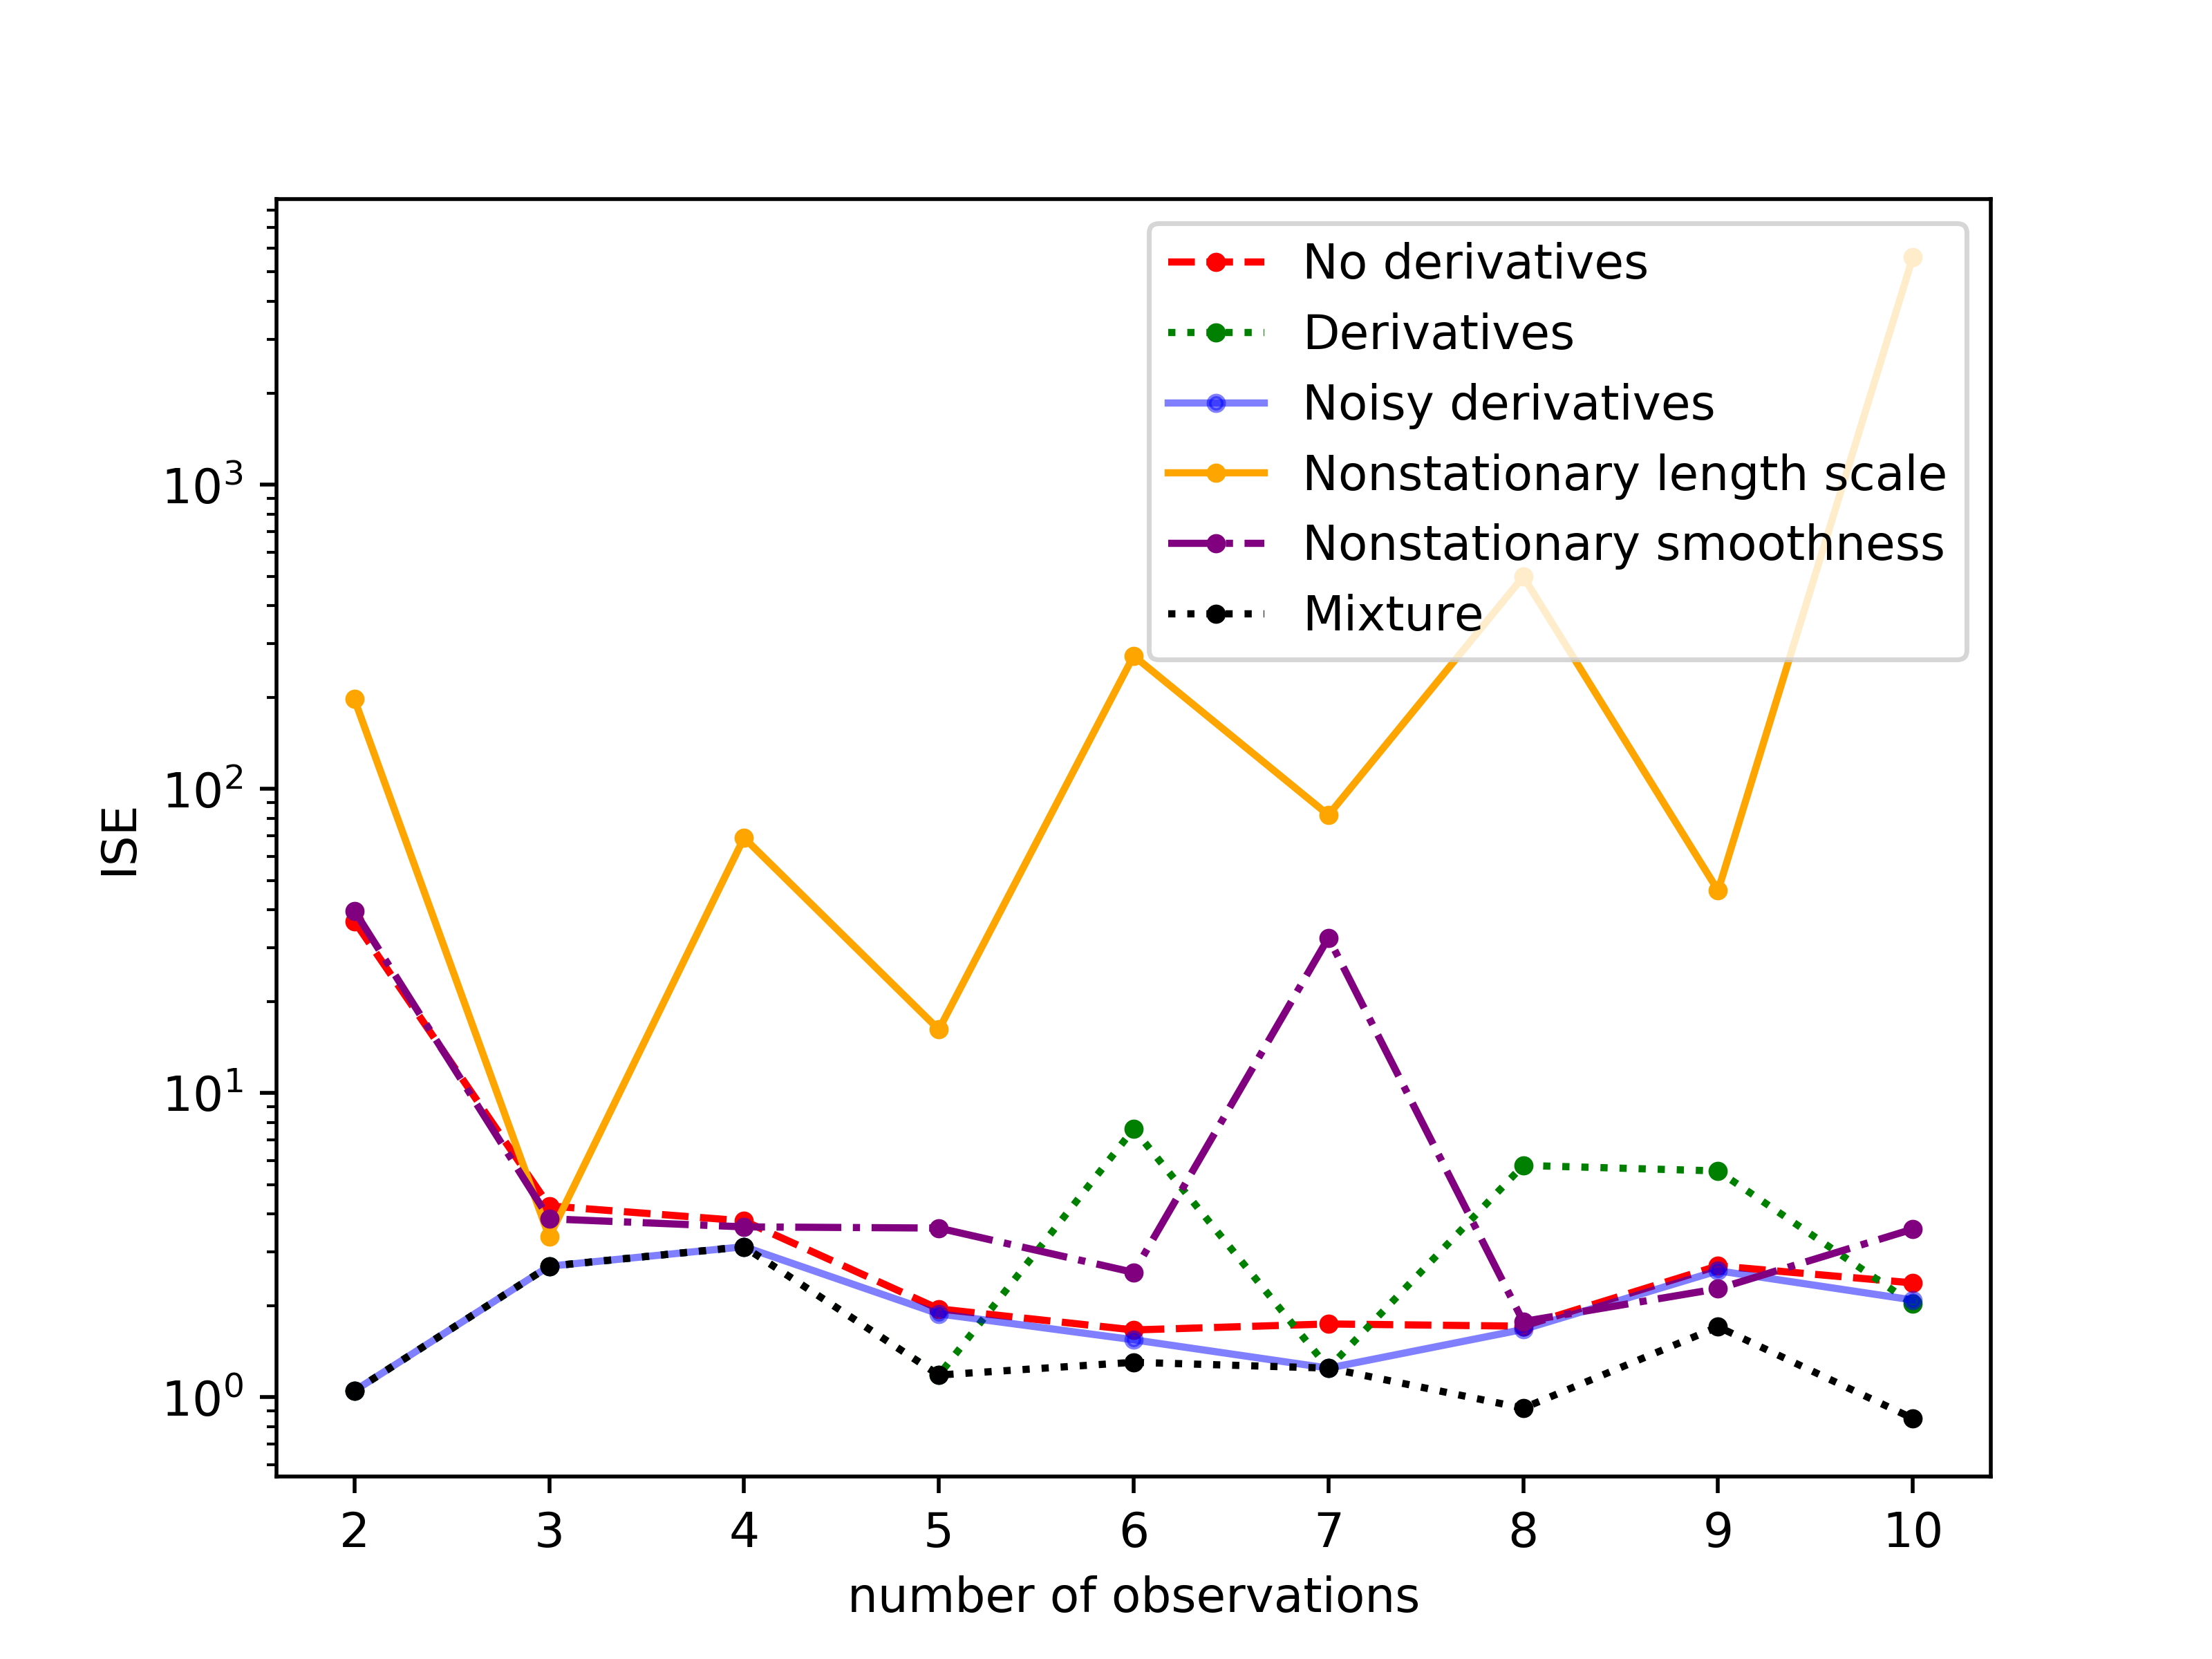
\includegraphics[scale=0.35]{figures/crazy-1D.png}
      \caption{\textbf{ISE in $\R$}}
    \end{subfigure}
    \begin{subfigure}[t]{.4\textwidth}
      \centering
      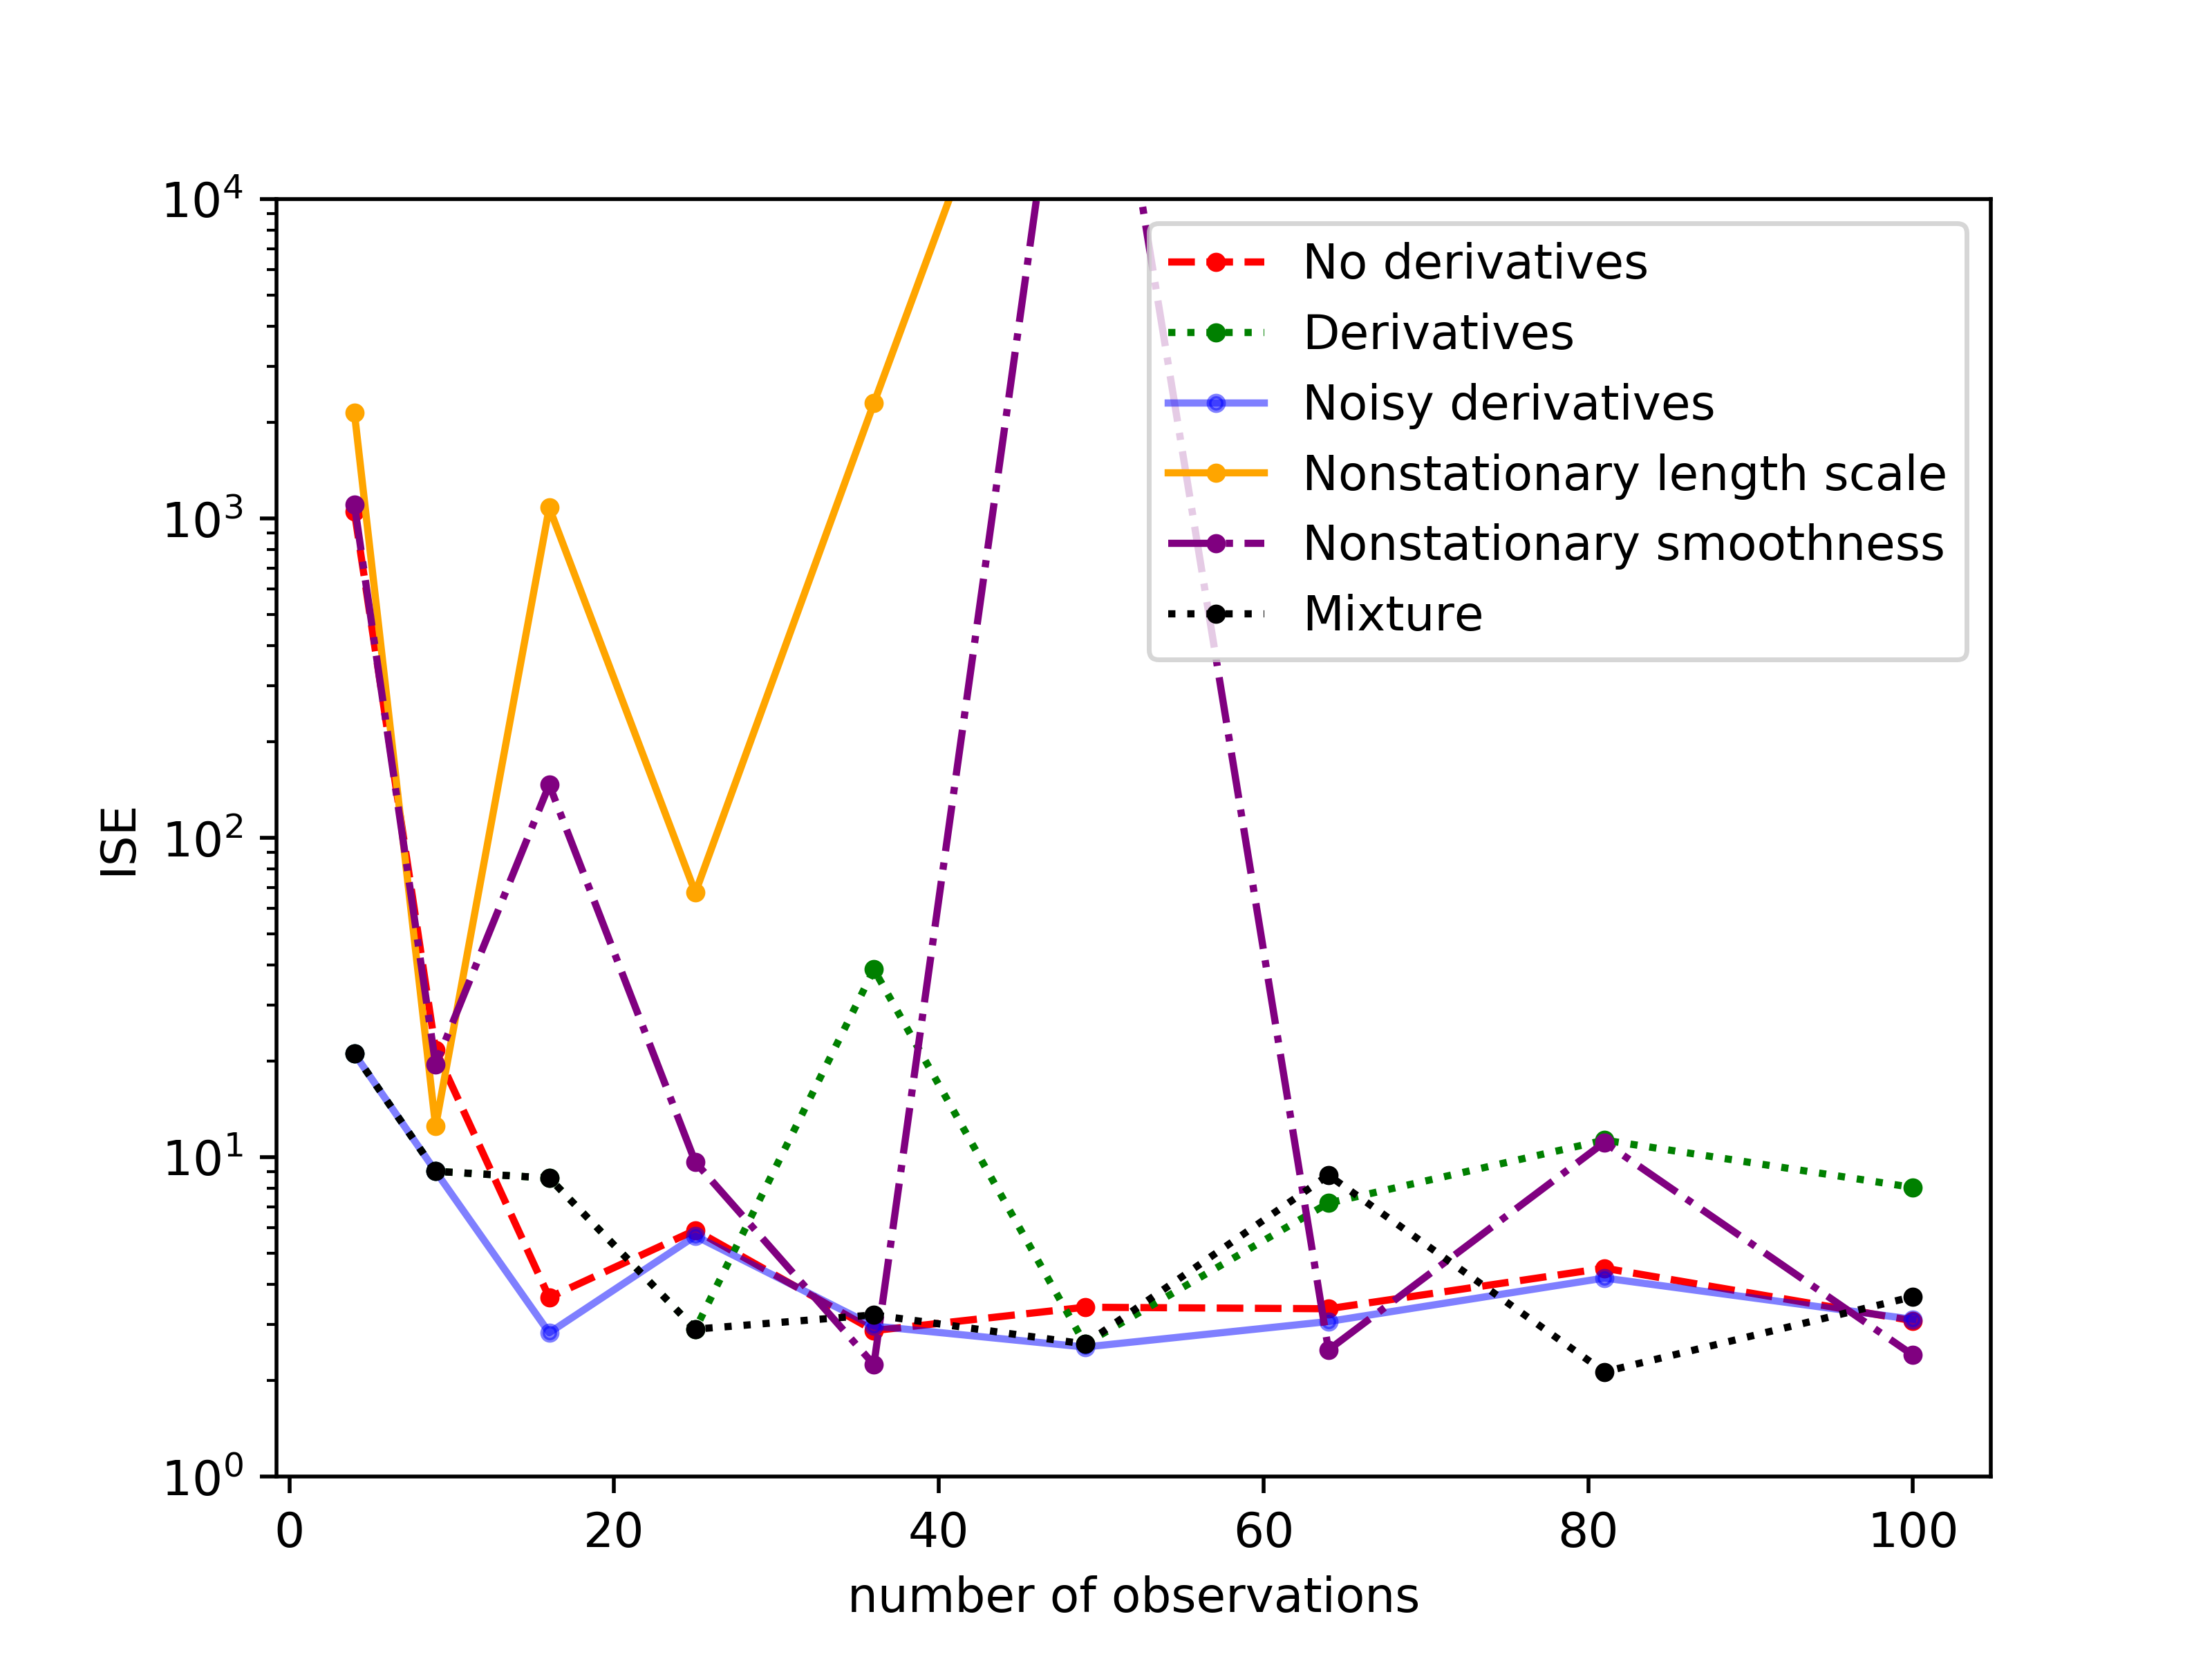
\includegraphics[scale=0.35]{figures/crazy-2D.png}
      \caption{\textbf{ISE in $\R^2$}}
    \end{subfigure}%
    \begin{subfigure}[t]{.4\textwidth}
      \centering
      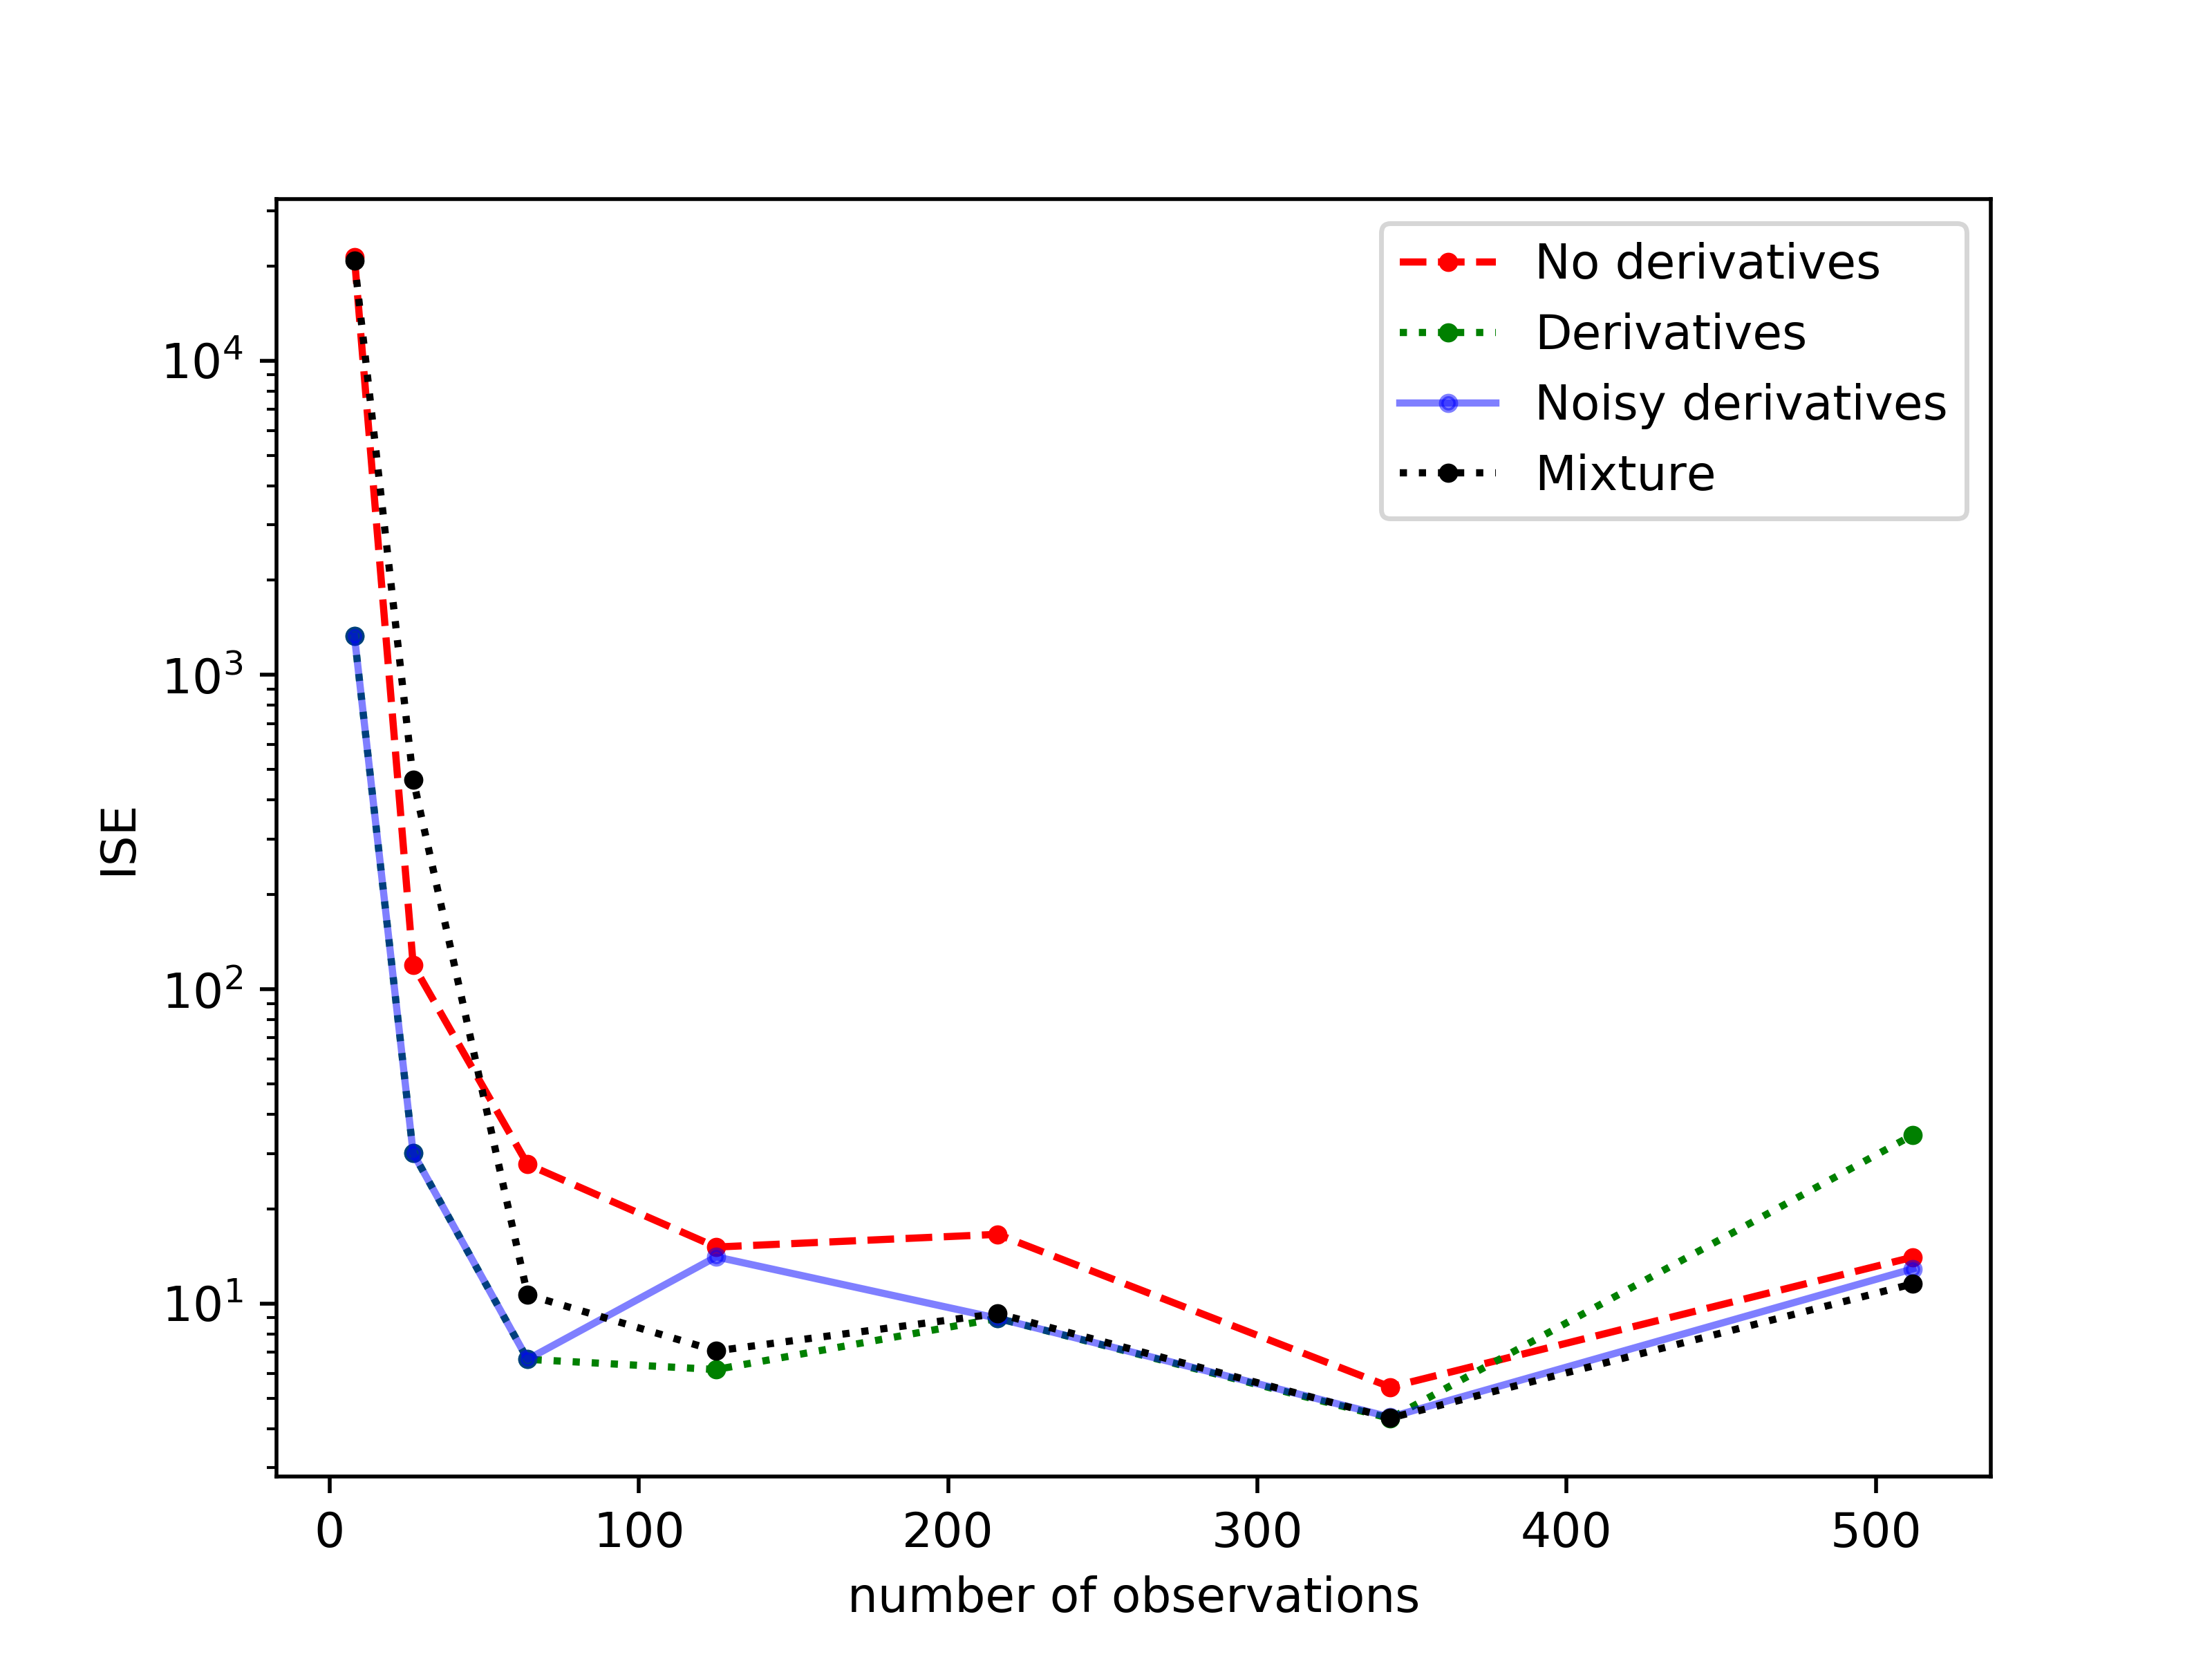
\includegraphics[scale=0.35]{figures/crazy-3D.png}
      \caption{\textbf{ISE in $\R^3$}}
    \end{subfigure}
		\caption{Integrated squared error between \texttt{rad2} and the GP posterior mean. Gaussian processes constructed from observations on regular grids.}
		\label{crazy}
\end{figure}

\subsection{Variance error comparison}
Beyond the accuracy of the posterior mean, we also study how well the posterior variance matches the true error. Many sequential design methods using Gaussian processes rely on the posterior variance as a measure of uncertainty, allowing targeted sampling of unexplored regions, see~\cite{jones1998efficient, ranjan2008sequential}. If the posterior variance does not match the true error, sequential designs may sample regions where the posterior mean is already a good estimator, which is significant loss when computational complexity limits the number of possible samples. Table~\ref{variance} compares the variance and true squared error of \texttt{rad1} using standard and gradient-interpolating GPS as well as our nonstationary approaches. Considering the expressions \eqref{eq:posterior-var} and \eqref{eq:posterior-var-der} for posterior variance with and without gradient observations, we see that without the introduction of nonstationary effects, the posterior variances depend only on the locations of the inputs. Thus for the standard and gradient-interpolating GPs, the regions of high variance are regularly spaced away from the inputs, while the largest errors occur in the annulus between circular kinks. While this high error region coincides with some regions of high posterior variance, there are a number of other high variance regions where the true error is in fact low and which may be explored first.

We also note that the posterior variance of the nonstationary smoothness method largely mimics the regular checkerboard patterns of the stationary methods, while the mixture method, the nonstationary length scale, and the additive derivate noise model show improved agreement between the error and posterior variance in many cases. In particular, the mixture method accurately identifies observations near a kink in the center of the input space and uses the nonsmooth expert, which results in increased variance. The posterior variance of the nonstationary length scale GP is largest at the edges of the input space, where the true error is also high. This is due to the fact that decreasing the length scale significantly increases the variance and thus regions in which the length scale has been reduced to avoid oscillation have higher variance.

The additive derivative noise model demonstrates increased posterior variance near kinks as added noise causes the posterior to resemble that of the standard GP rather than the gradient-interpolating GP as discussed in Section~\ref{ADN}. However, the difference between posterior variances in standard and gradient-interpolating GPs can be subtle. To assure that nondifferentiable regions are adequately sampled, one could explicitly include branching distance as a component of a sequential design metric in addition to posterior variance, increasing the probability of sampling near kinks as these regions are the most likely to suffer from poor approximation. Such considerations remain for future work.

\begin{table}
  \centering
  \captionsetup{justification=centering}
  \begin{tabularx}{\textwidth}{| X | p{.18\textwidth} p{.18\textwidth} || p{.18\textwidth} p{.18\textwidth} |}
    \hline
    & \multicolumn{4}{c|}{\textbf{observations}} \\
    \hline
    \centering \textbf{method} & \multicolumn{2}{c||}{16} & \multicolumn{2}{c|}{25} \\
    \hline \hline
    \centering \textbf{Standard GP} &
      \parbox[c]{.18\textwidth}{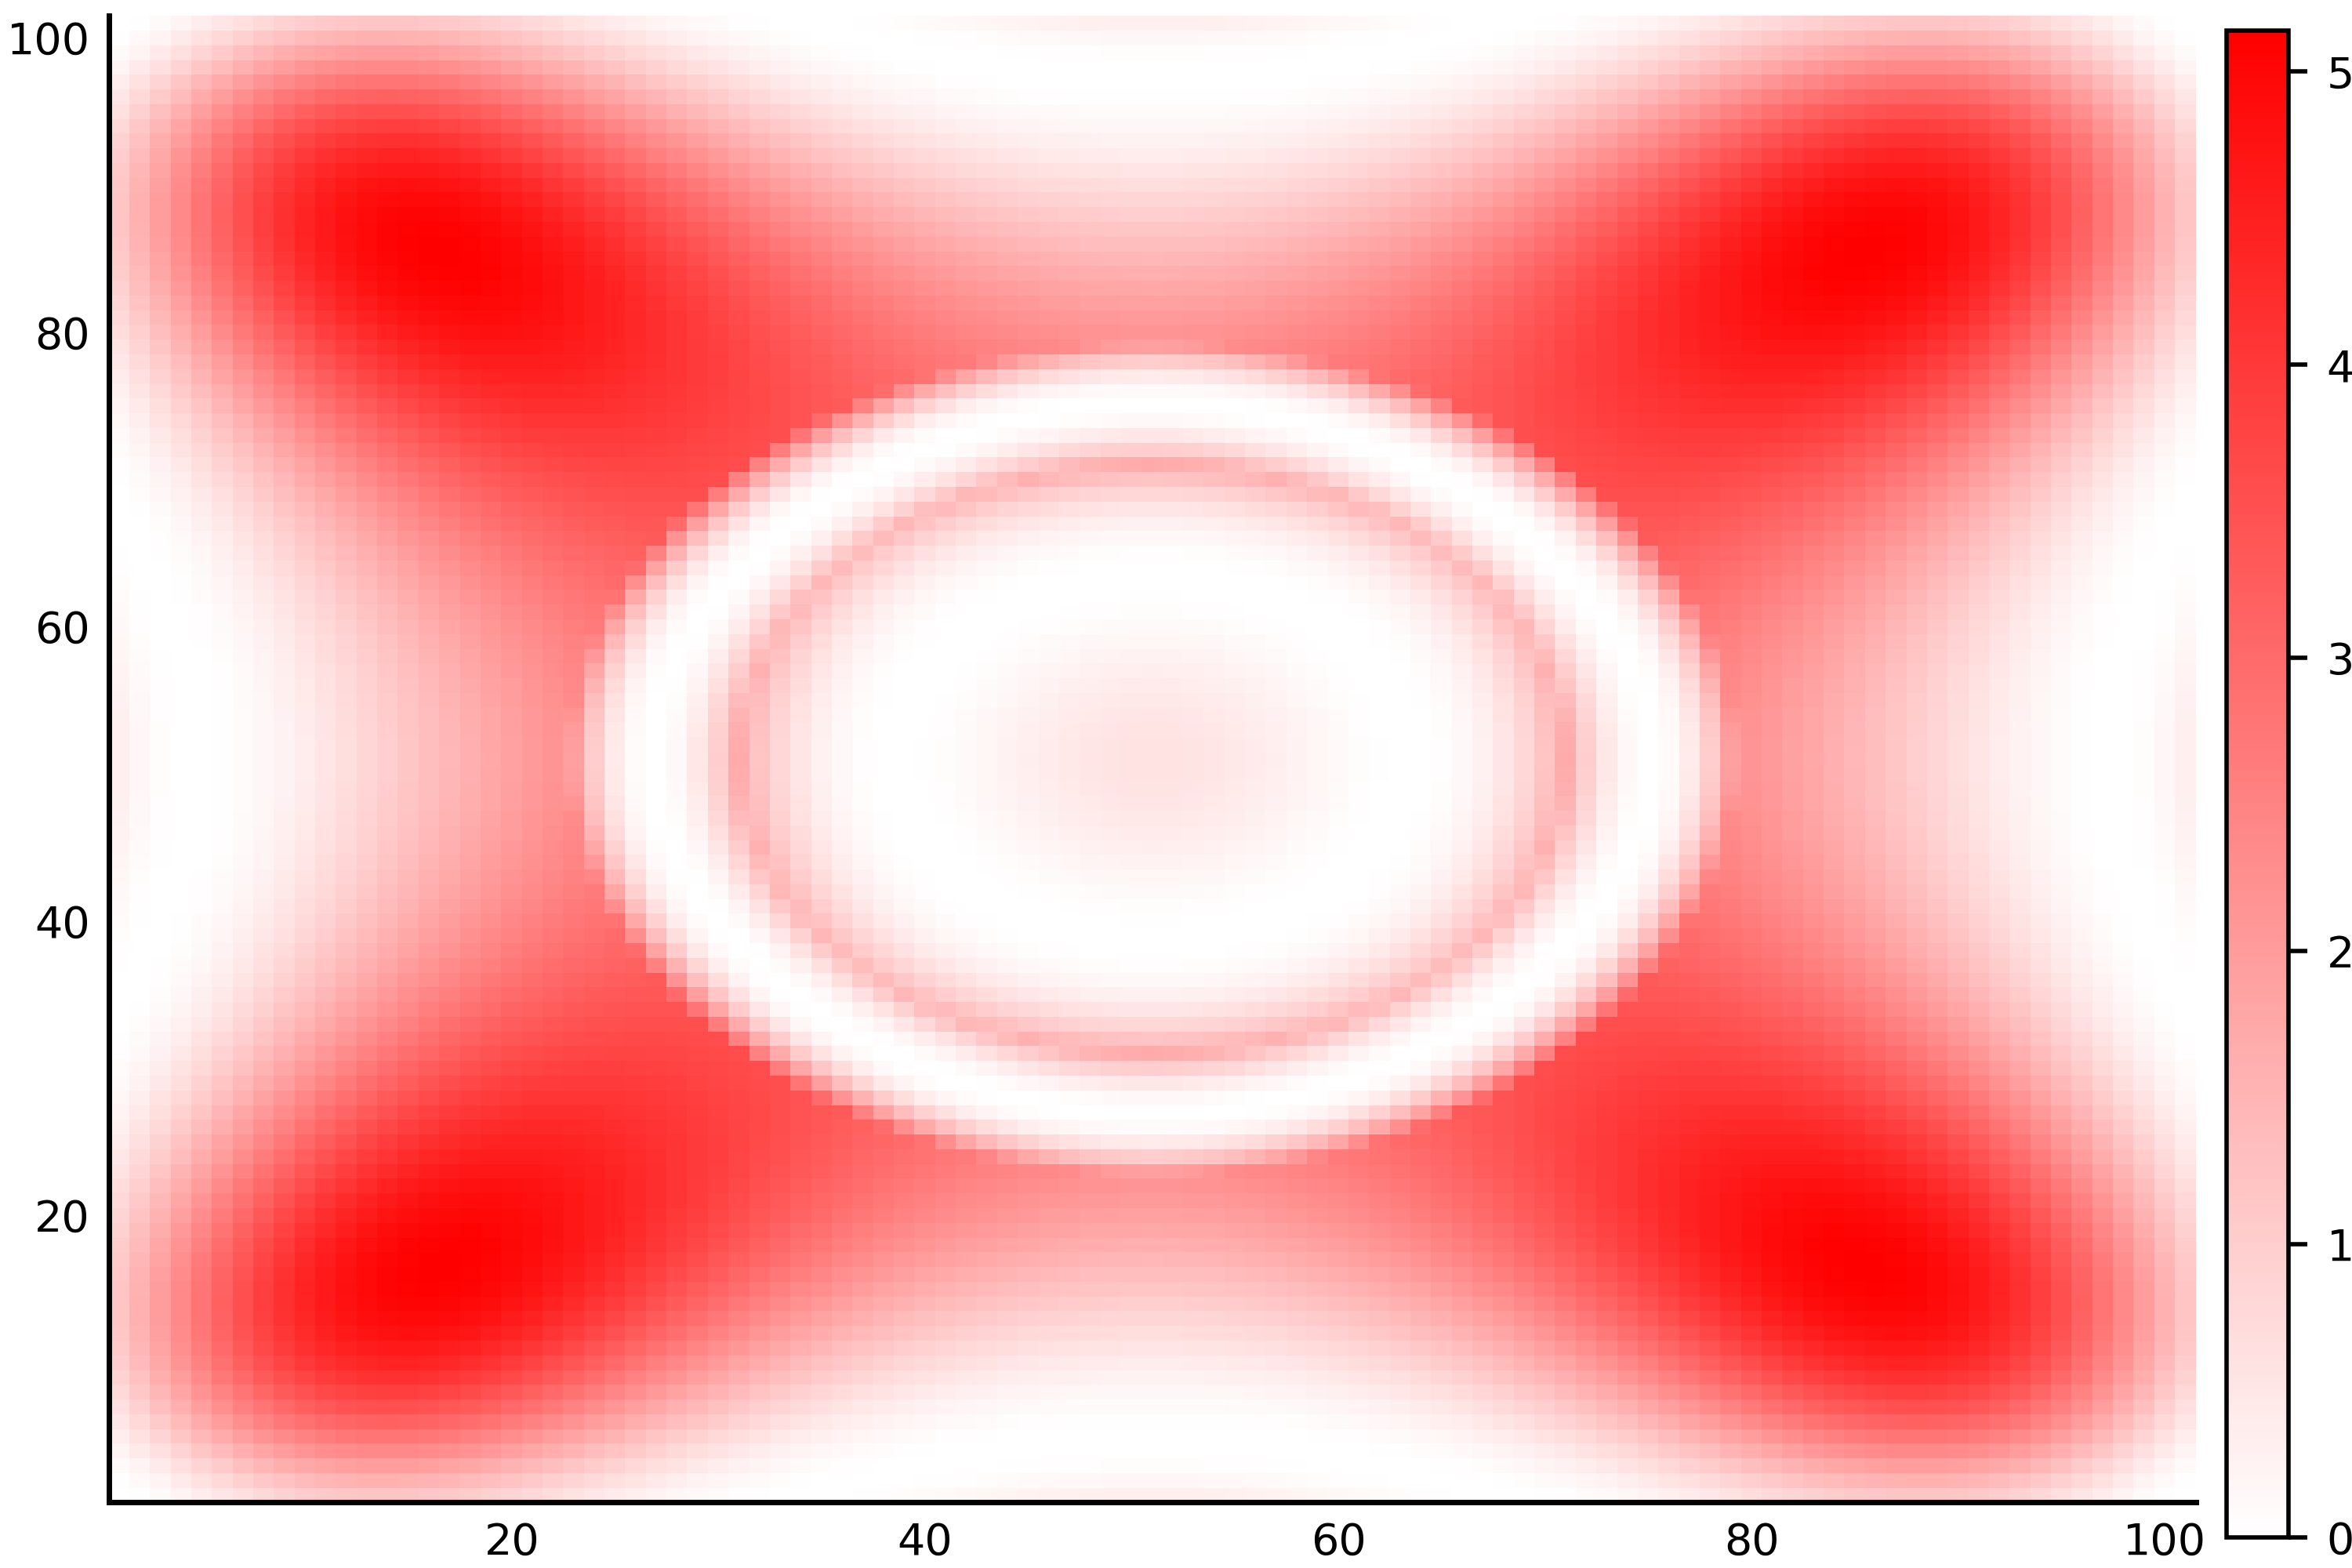
\includegraphics[scale=0.2]{figures/heatmaps/error-noder-16.png}} &
      \parbox[c]{.18\textwidth}{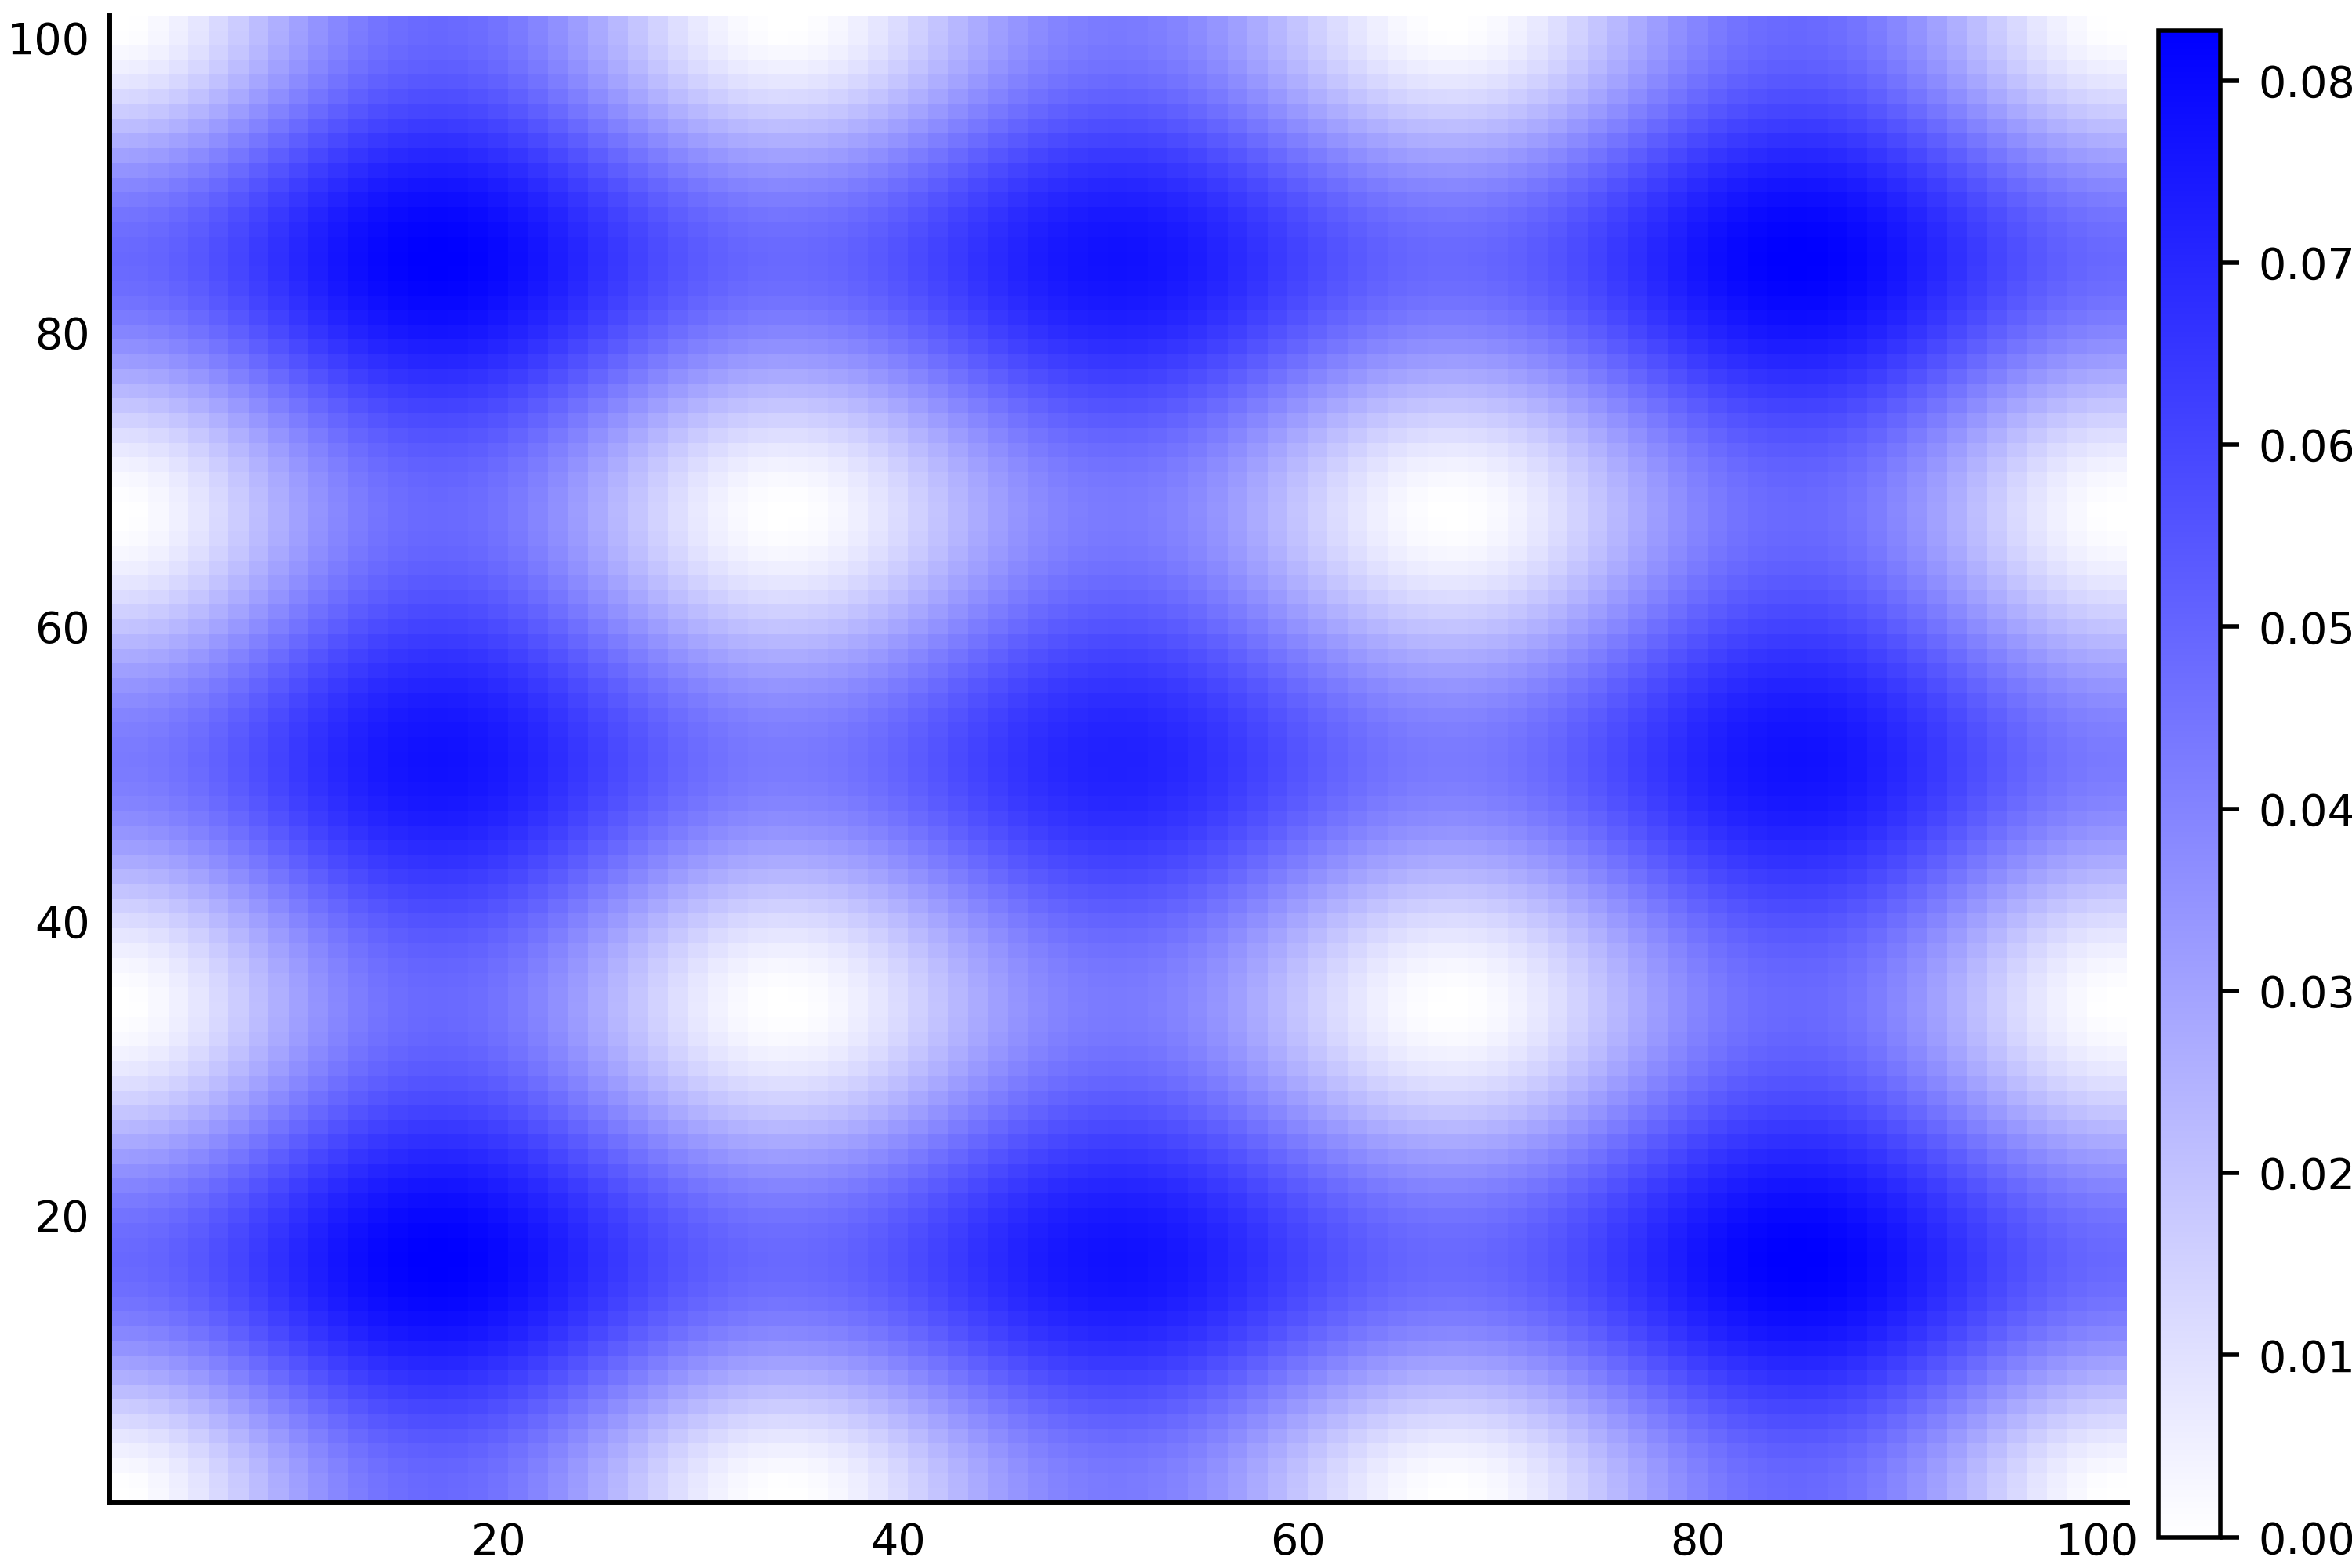
\includegraphics[scale=0.2]{figures/heatmaps/variance-noder-16.png}} &
      \parbox[c]{.18\textwidth}{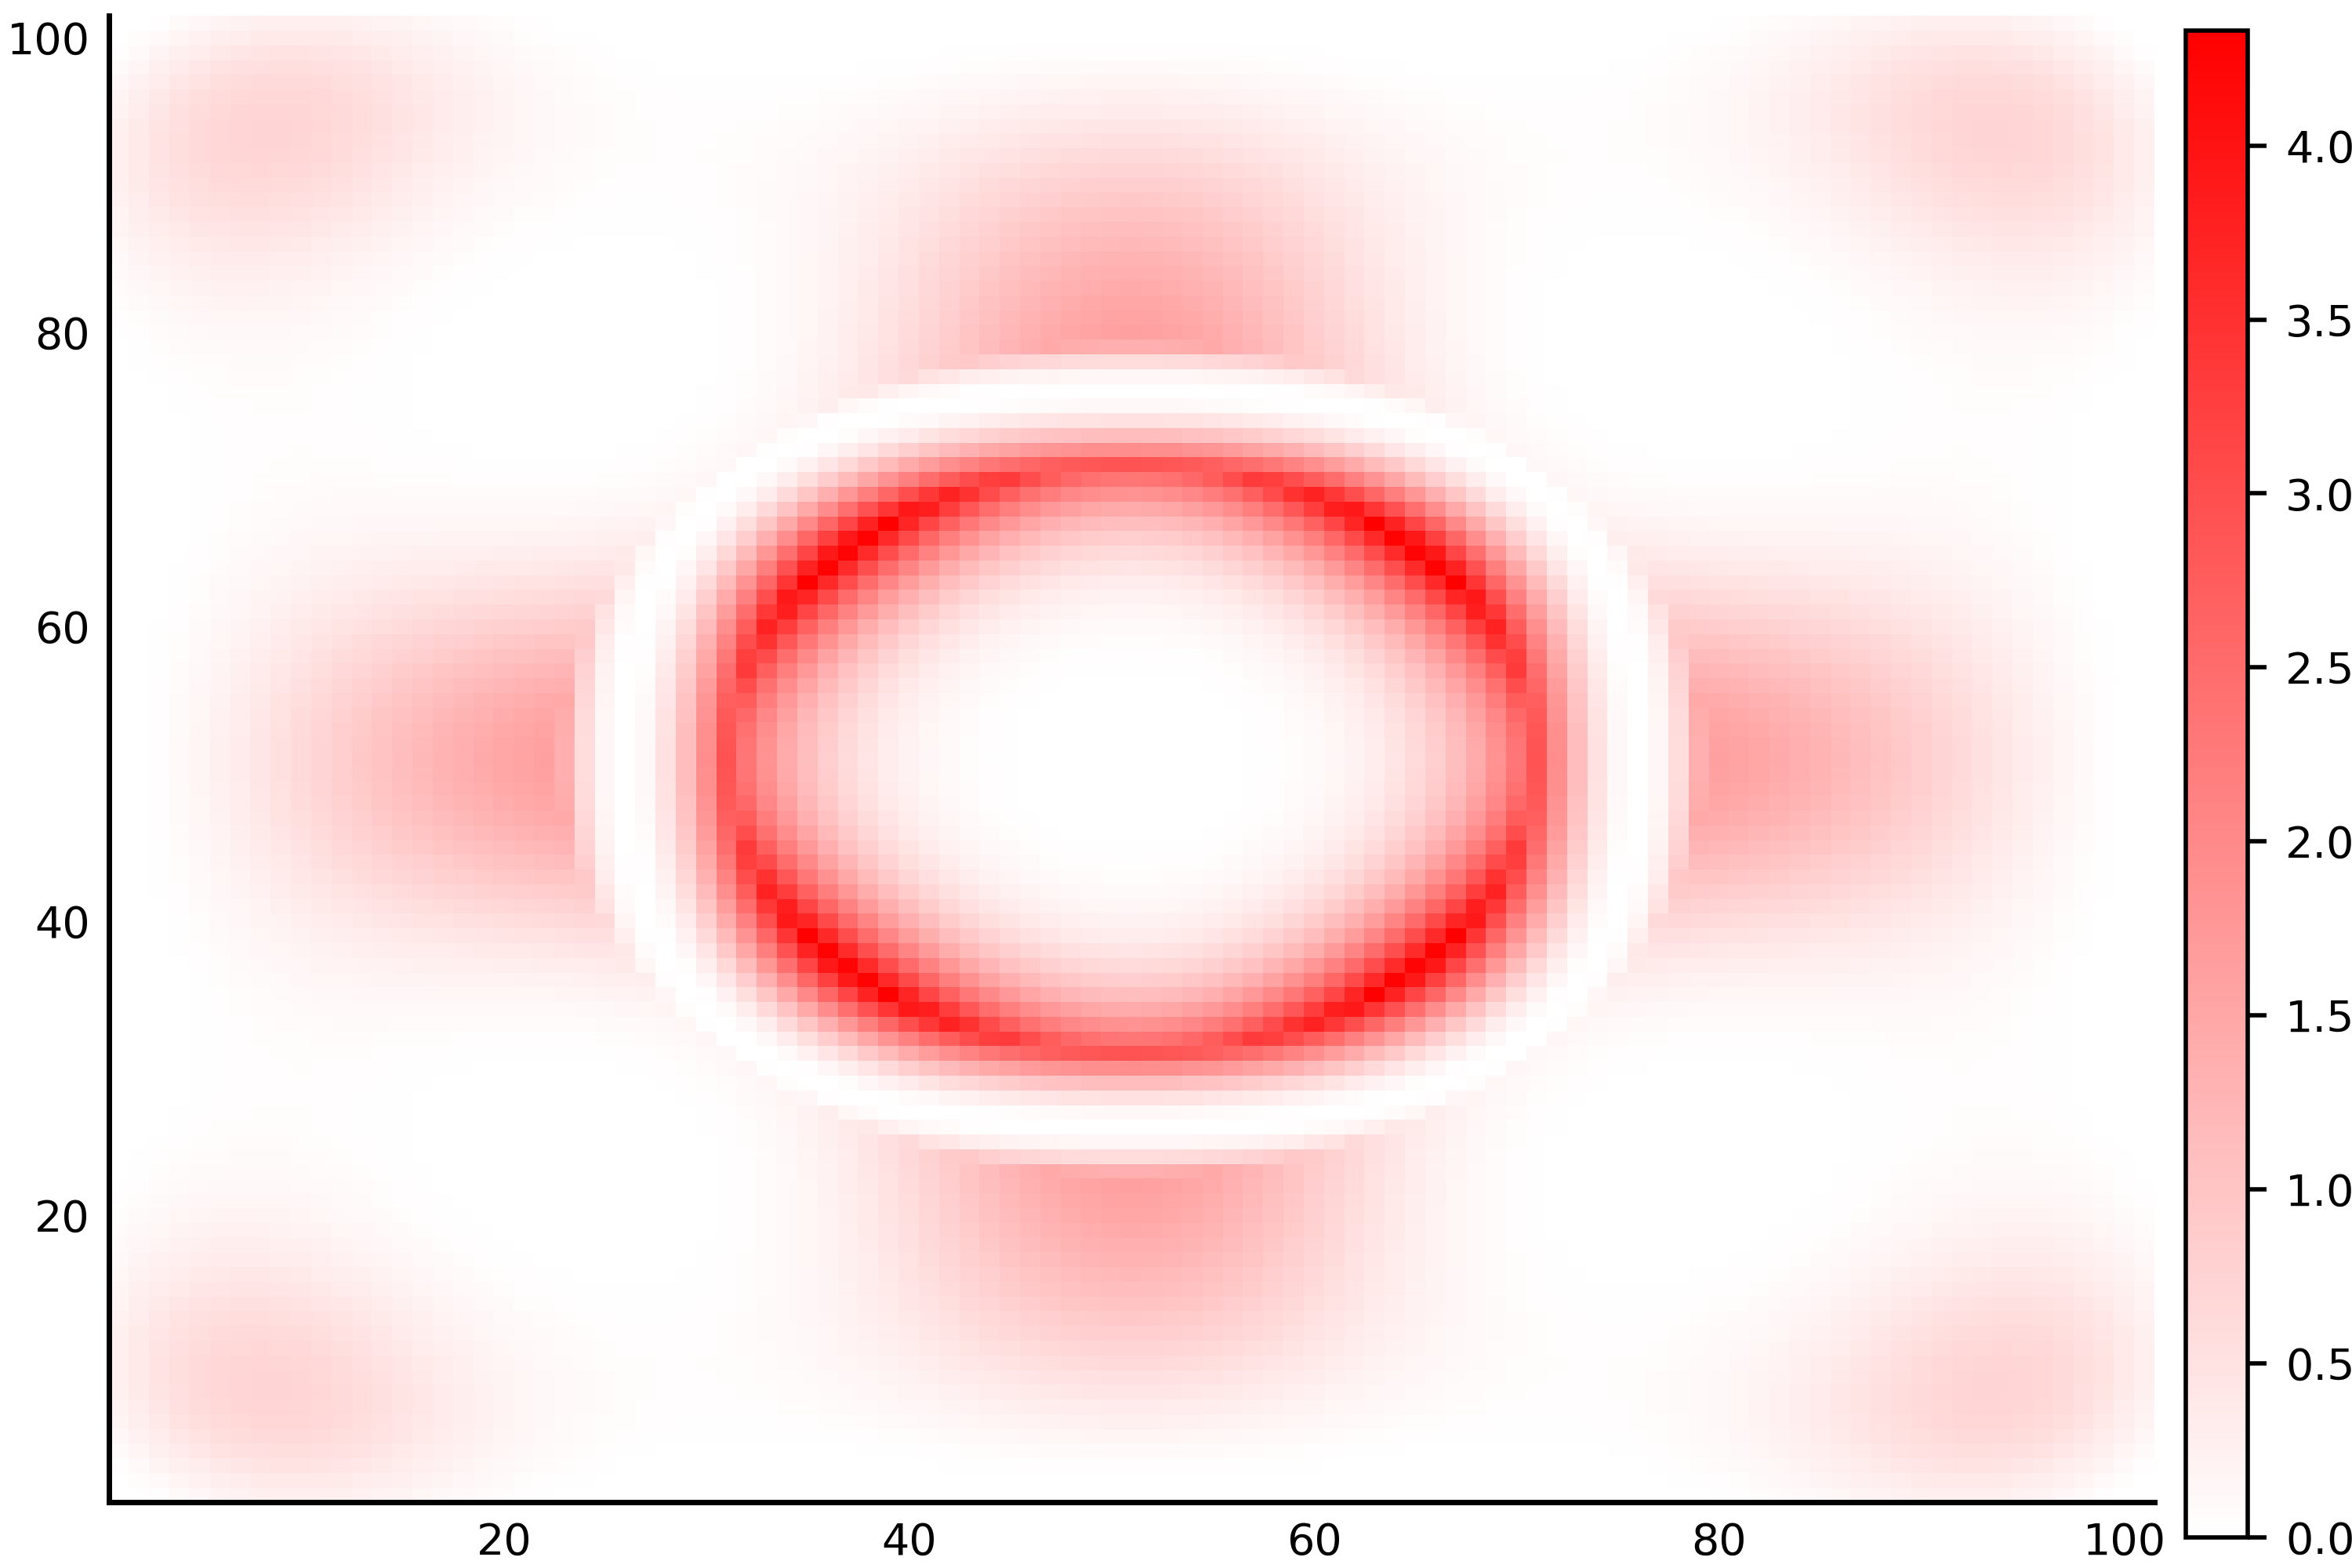
\includegraphics[scale=0.2]{figures/heatmaps/error-noder-25.png}} &
      \parbox[c]{.18\textwidth}{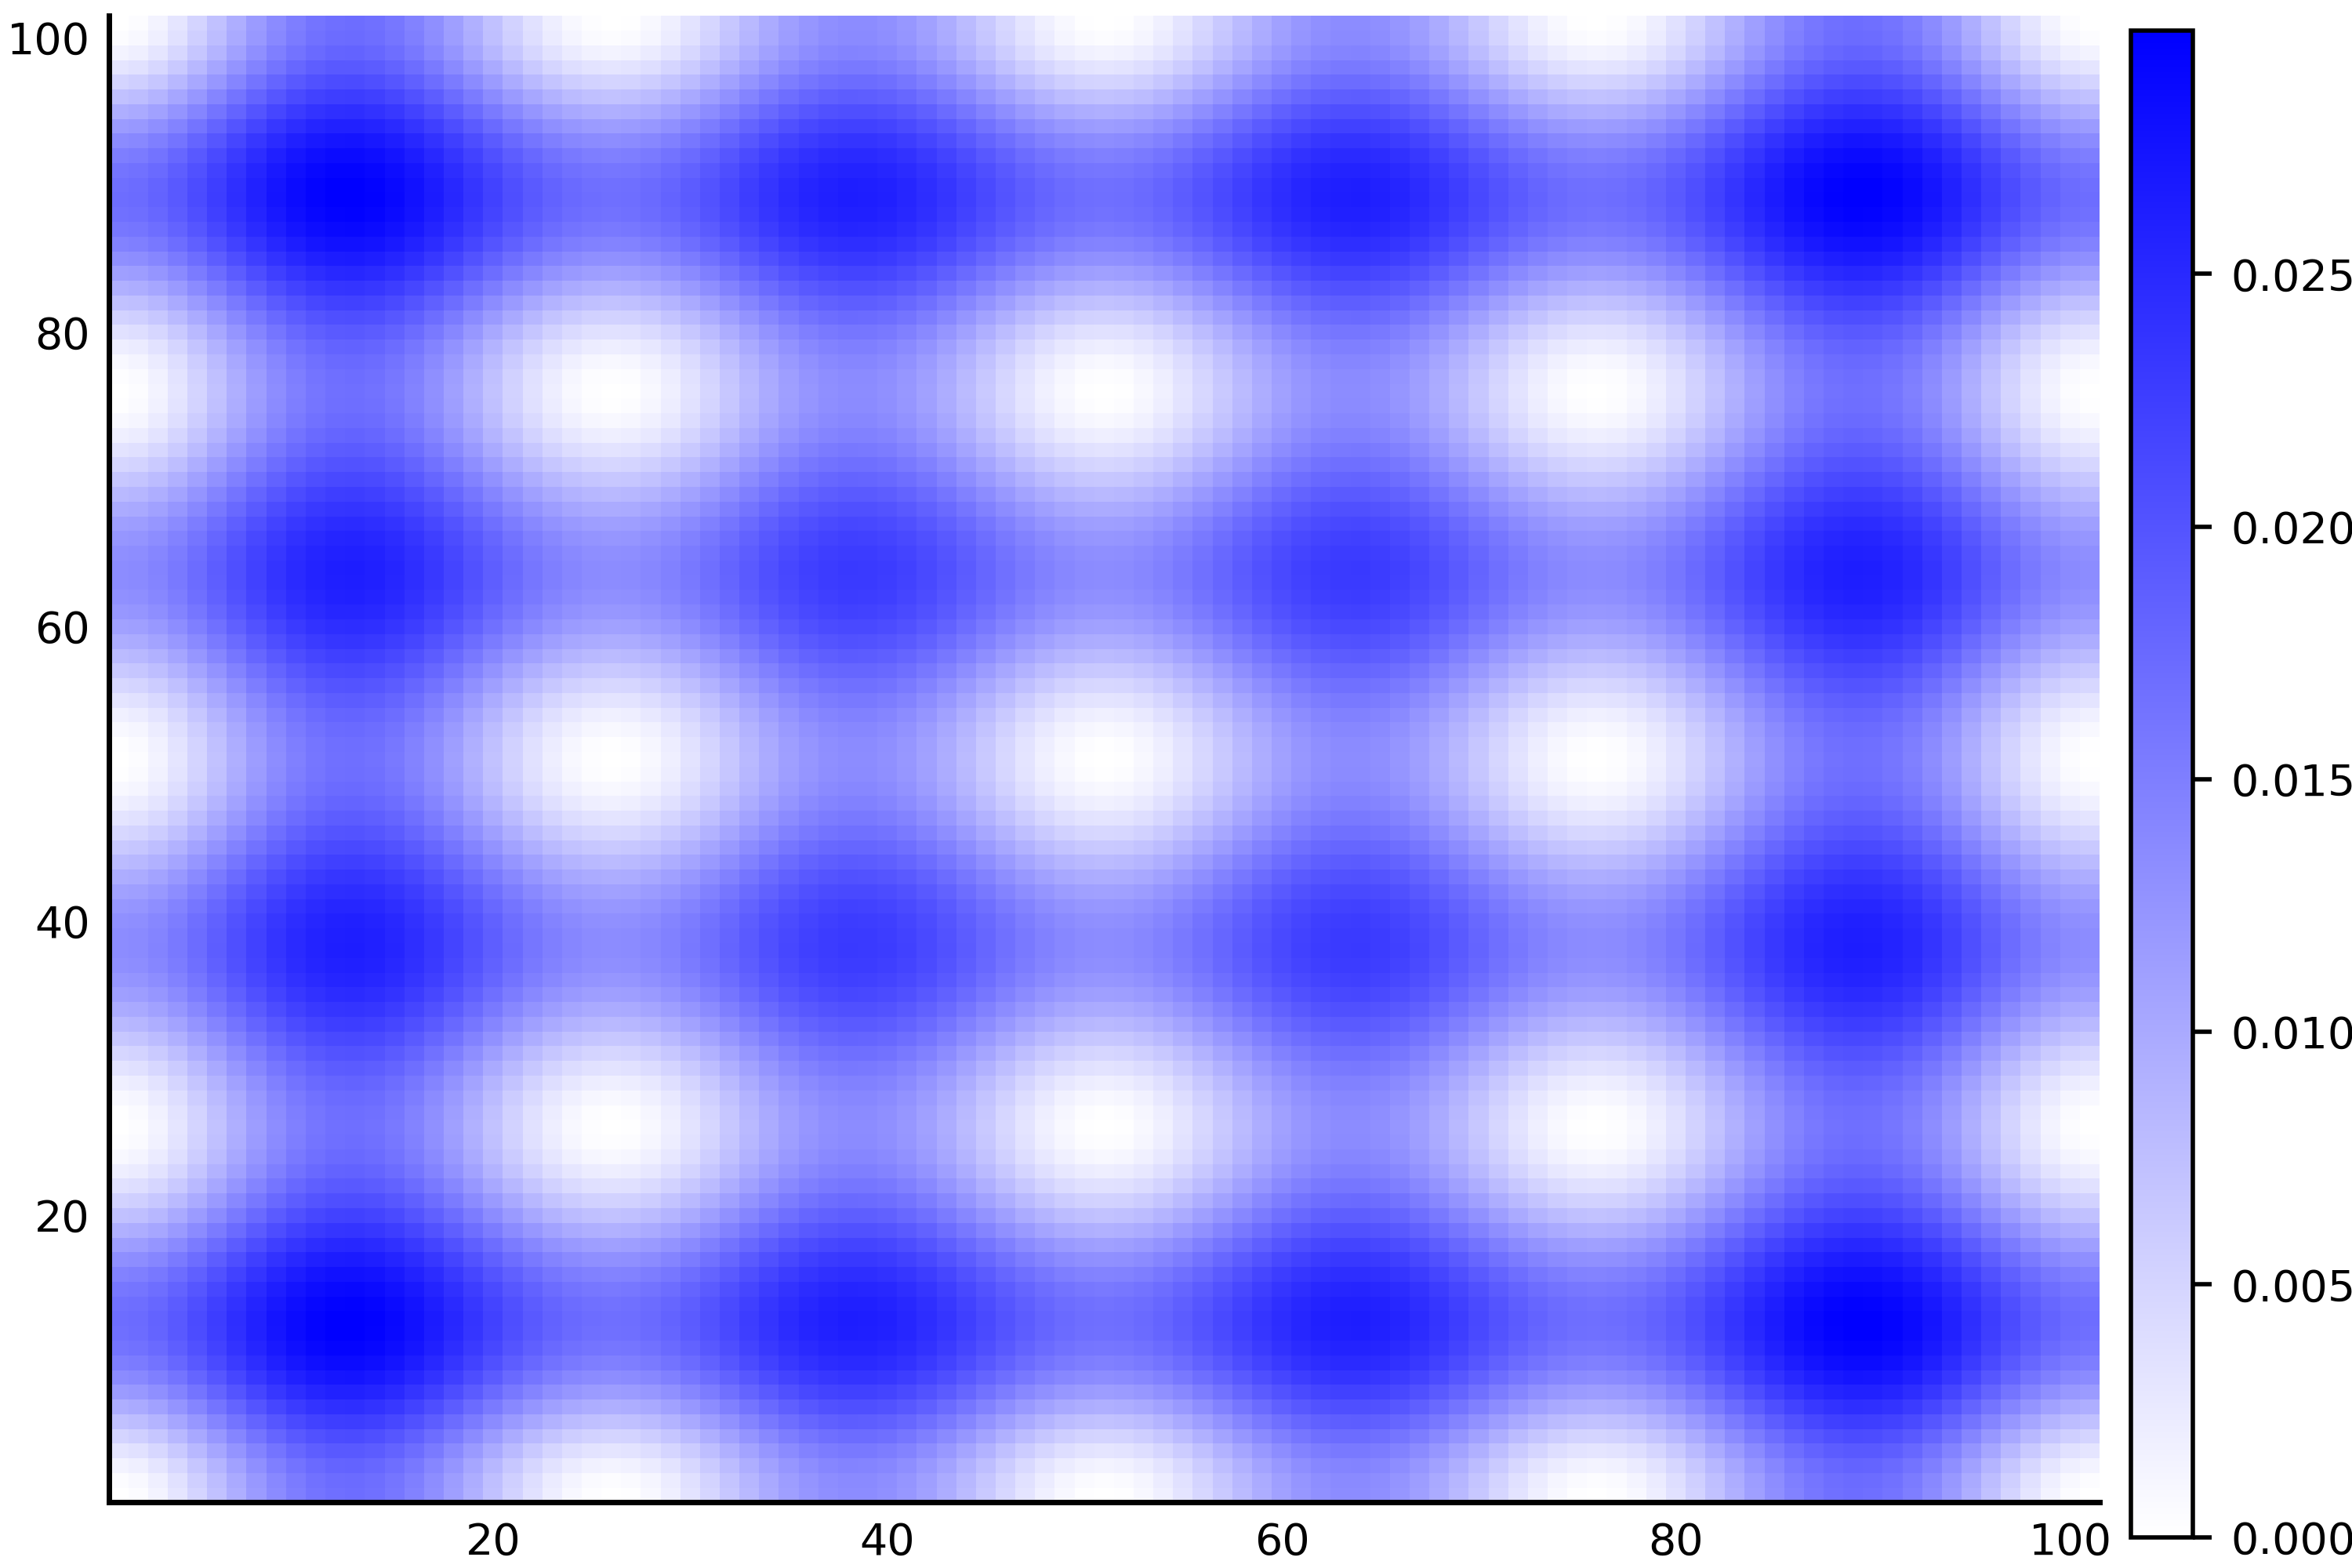
\includegraphics[scale=0.2]{figures/heatmaps/variance-noder-25.png}} \\
    \hline
    \centering \textbf{Gradient-interpolating GP} &
      \parbox[c]{.18\textwidth}{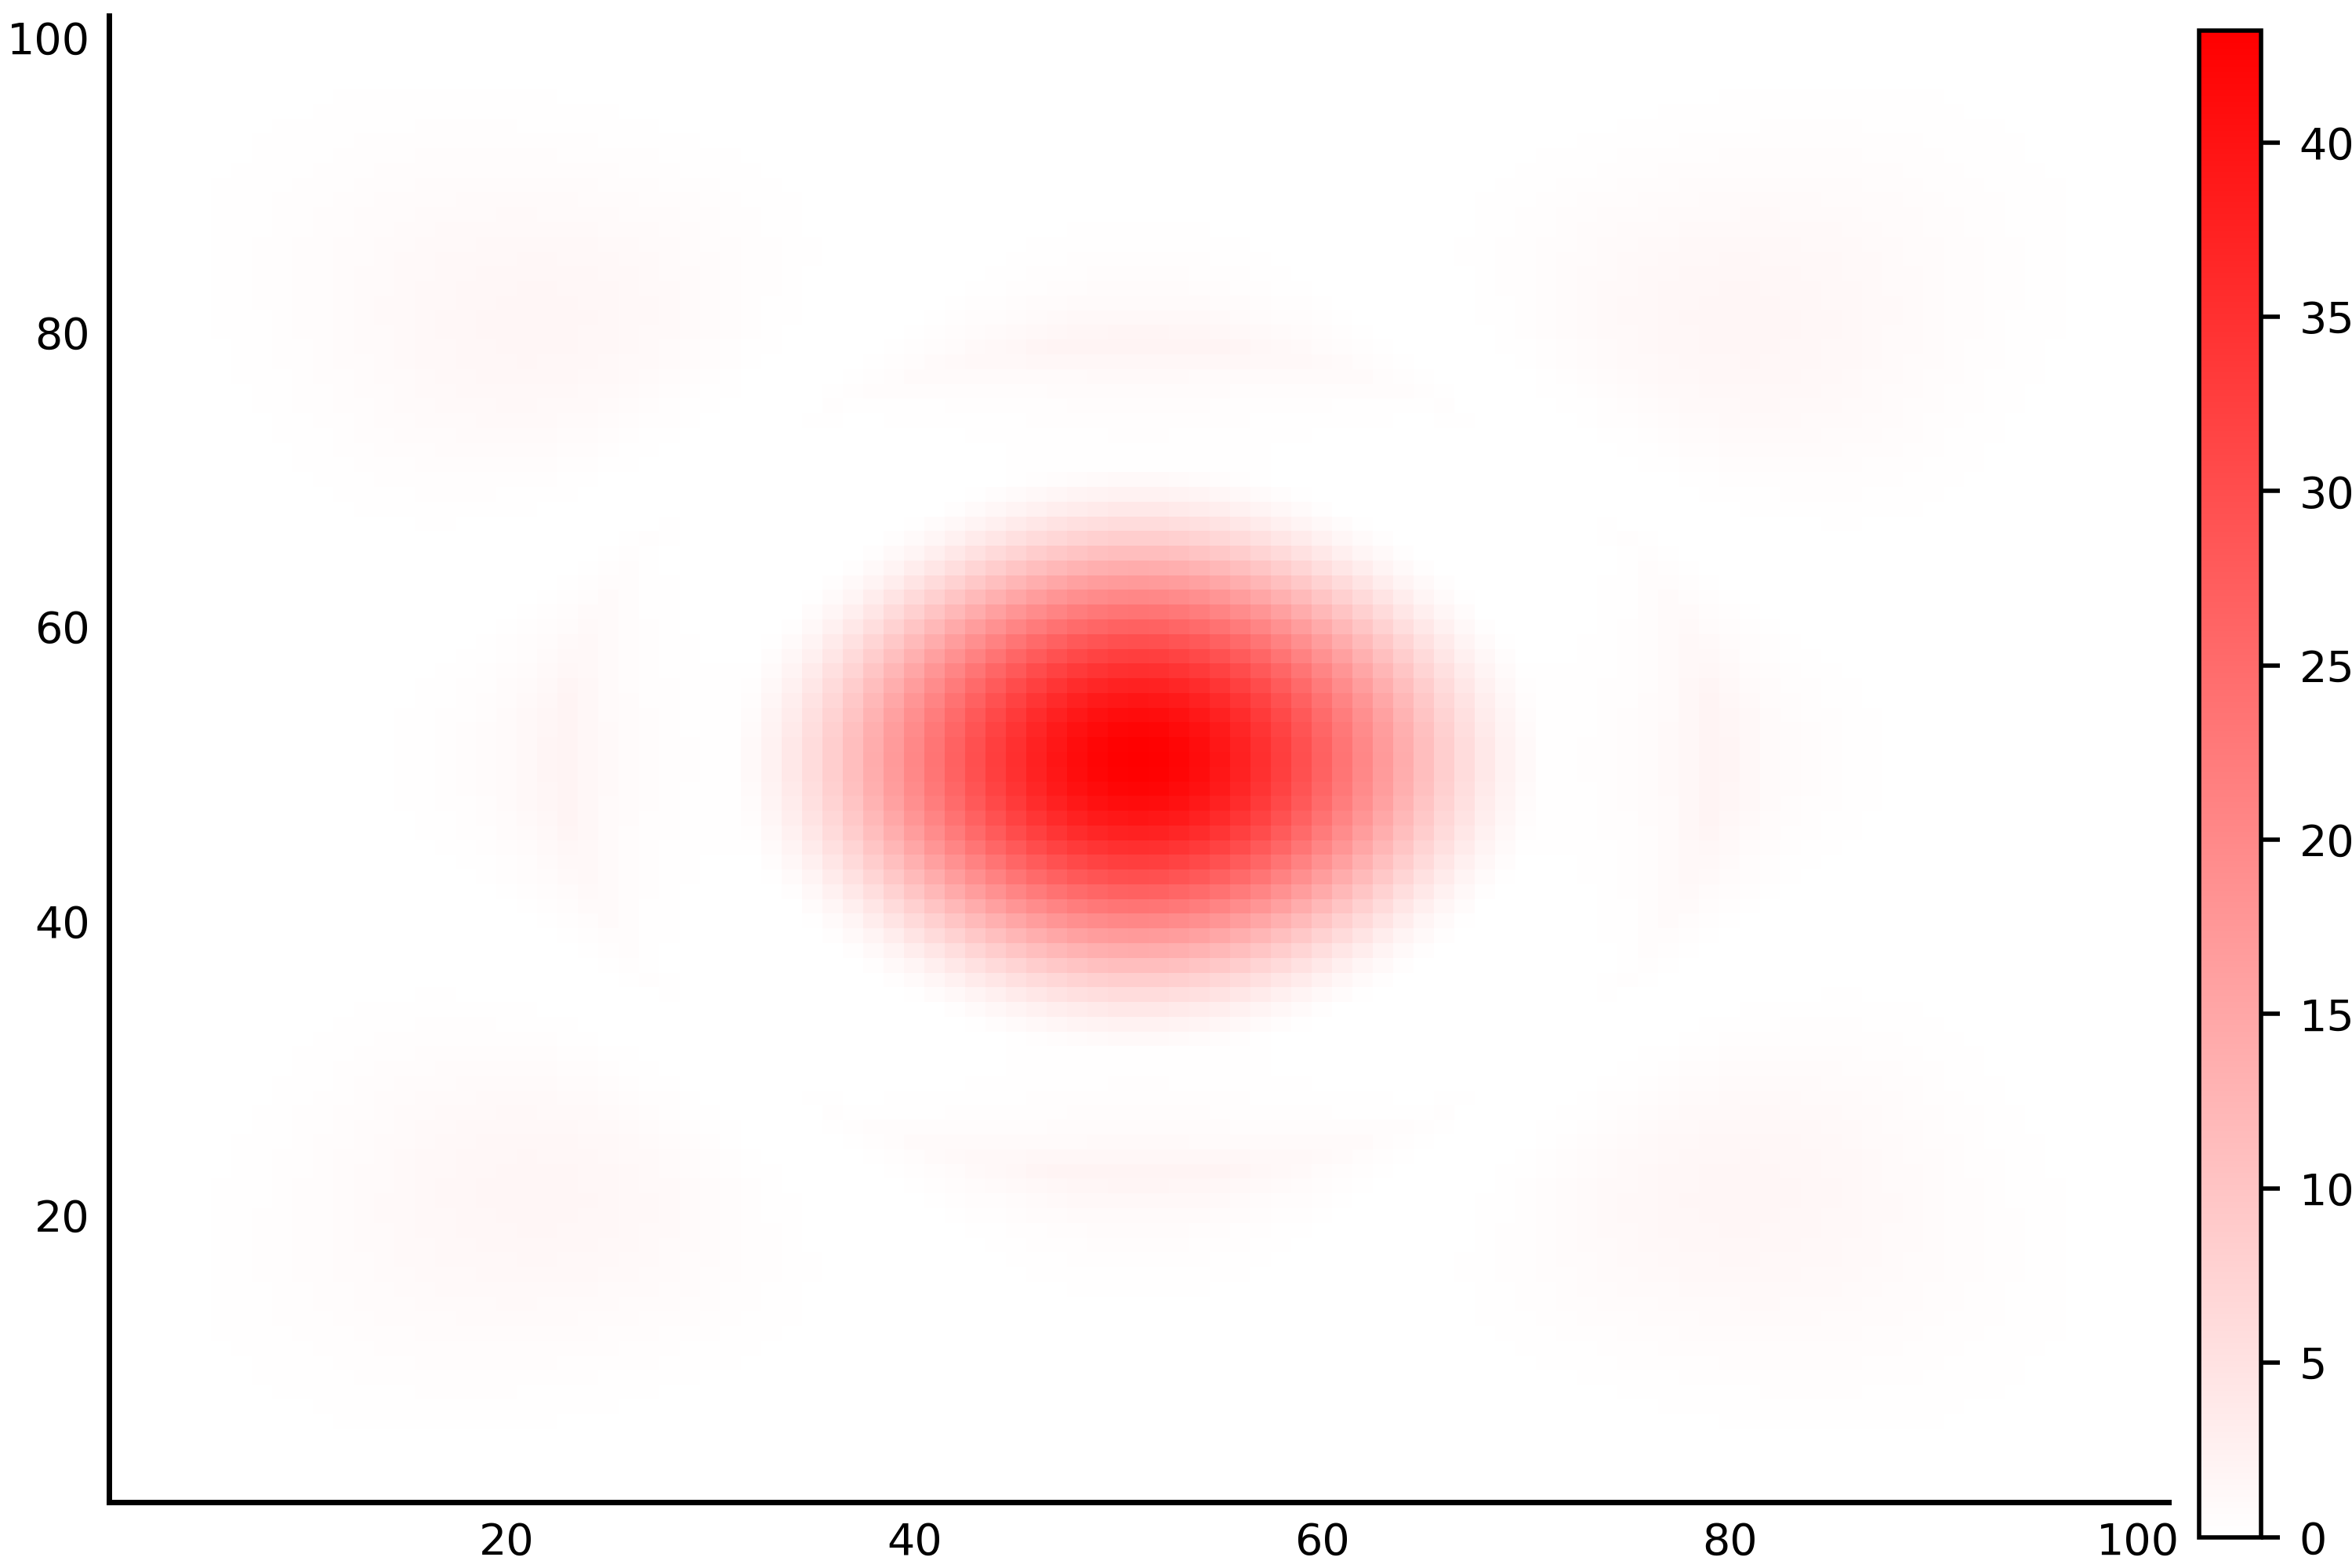
\includegraphics[scale=0.2]{figures/heatmaps/error-der-16.png}} &
      \parbox[c]{.18\textwidth}{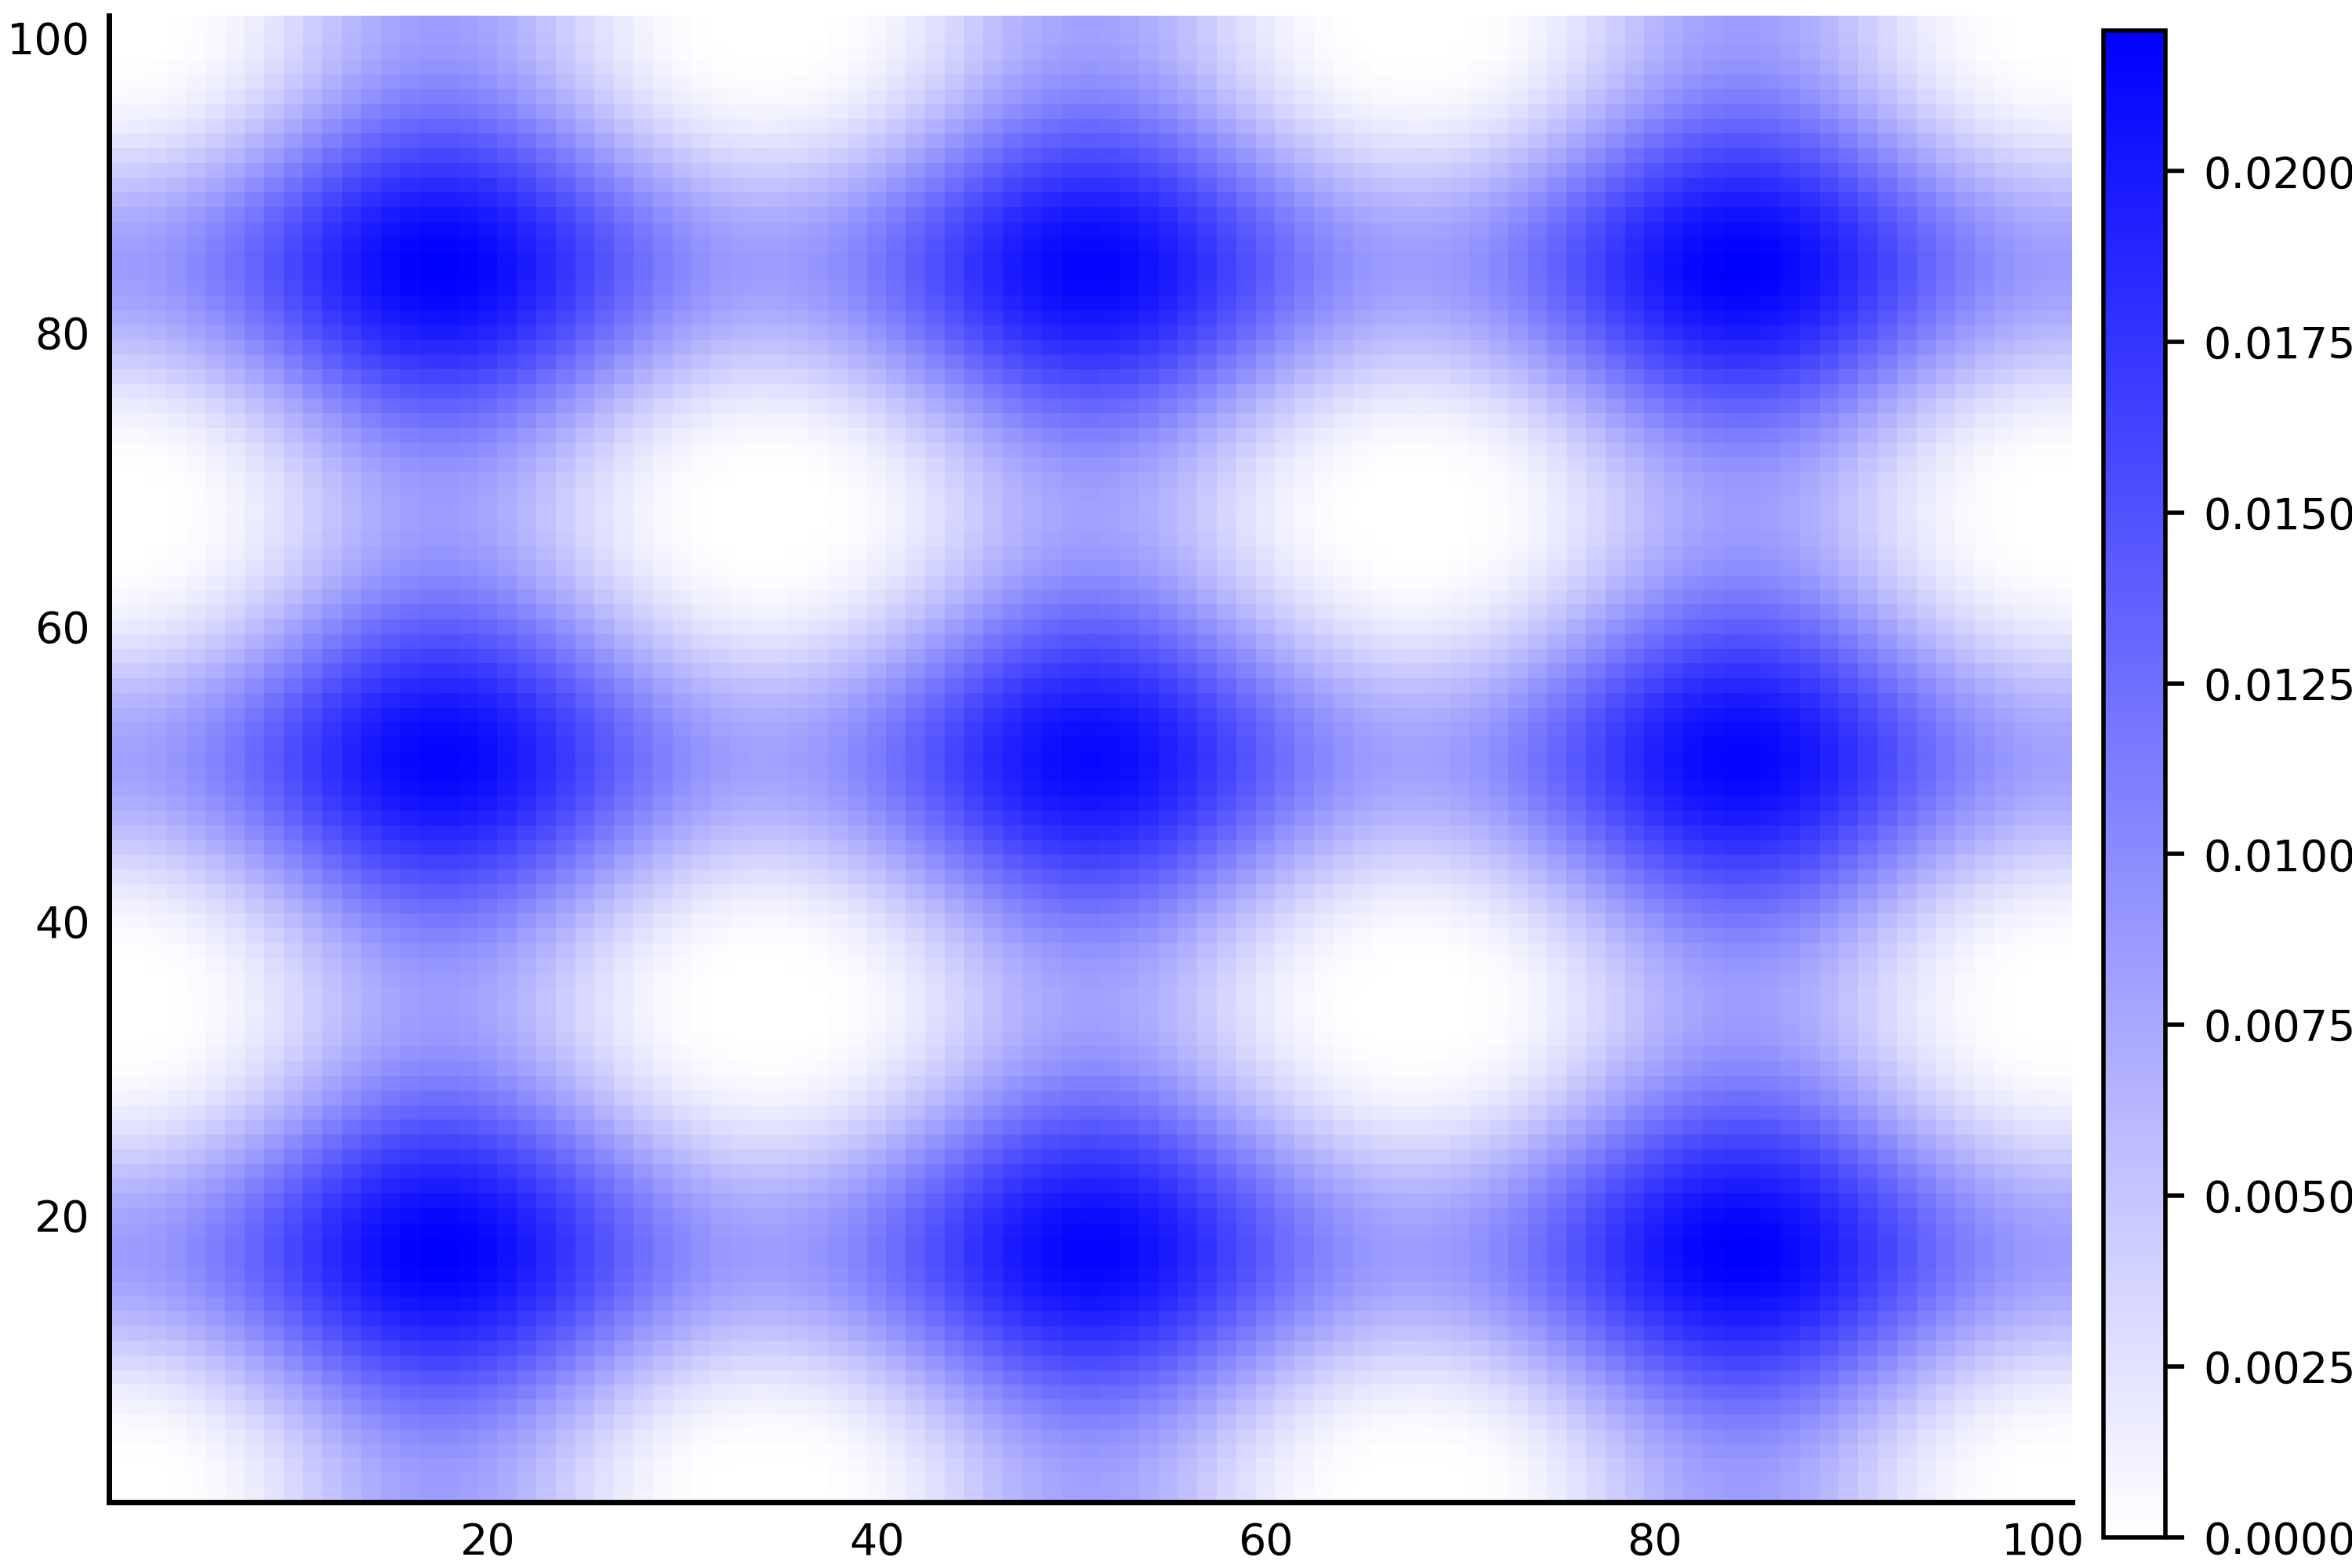
\includegraphics[scale=0.2]{figures/heatmaps/variance-der-16.png}} &
      \parbox[c]{.18\textwidth}{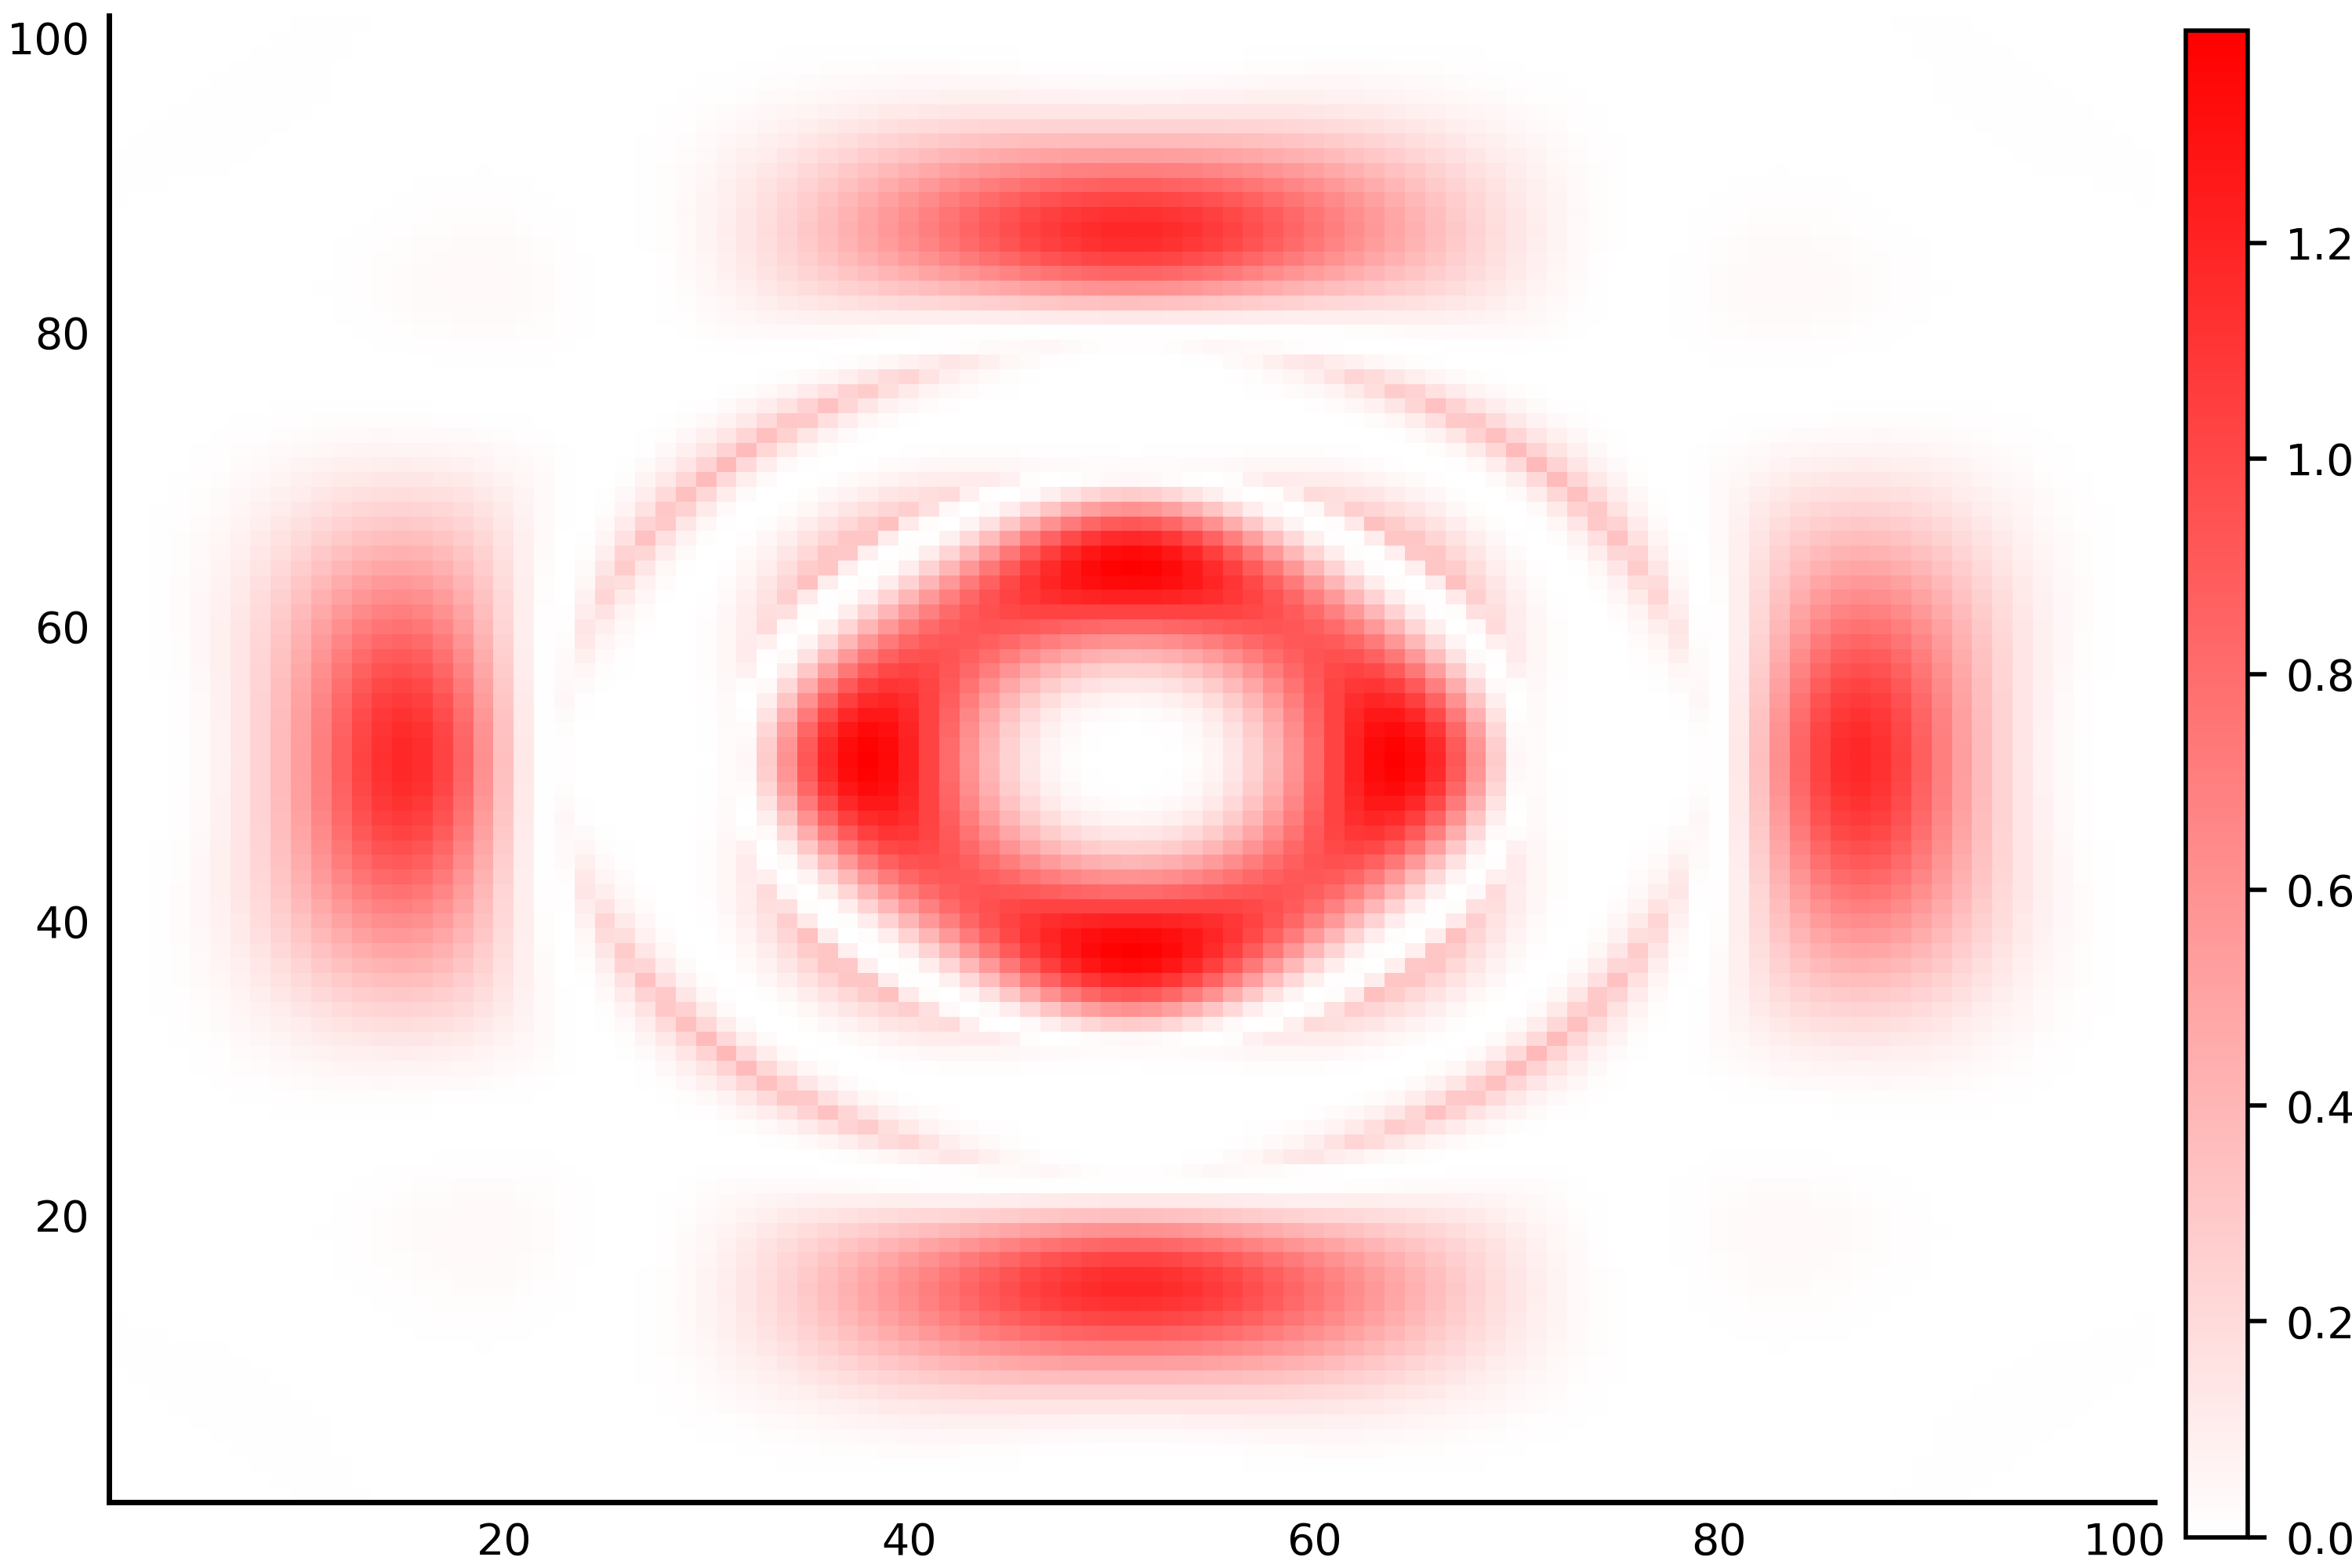
\includegraphics[scale=0.2]{figures/heatmaps/error-der-25.png}} &
      \parbox[c]{.18\textwidth}{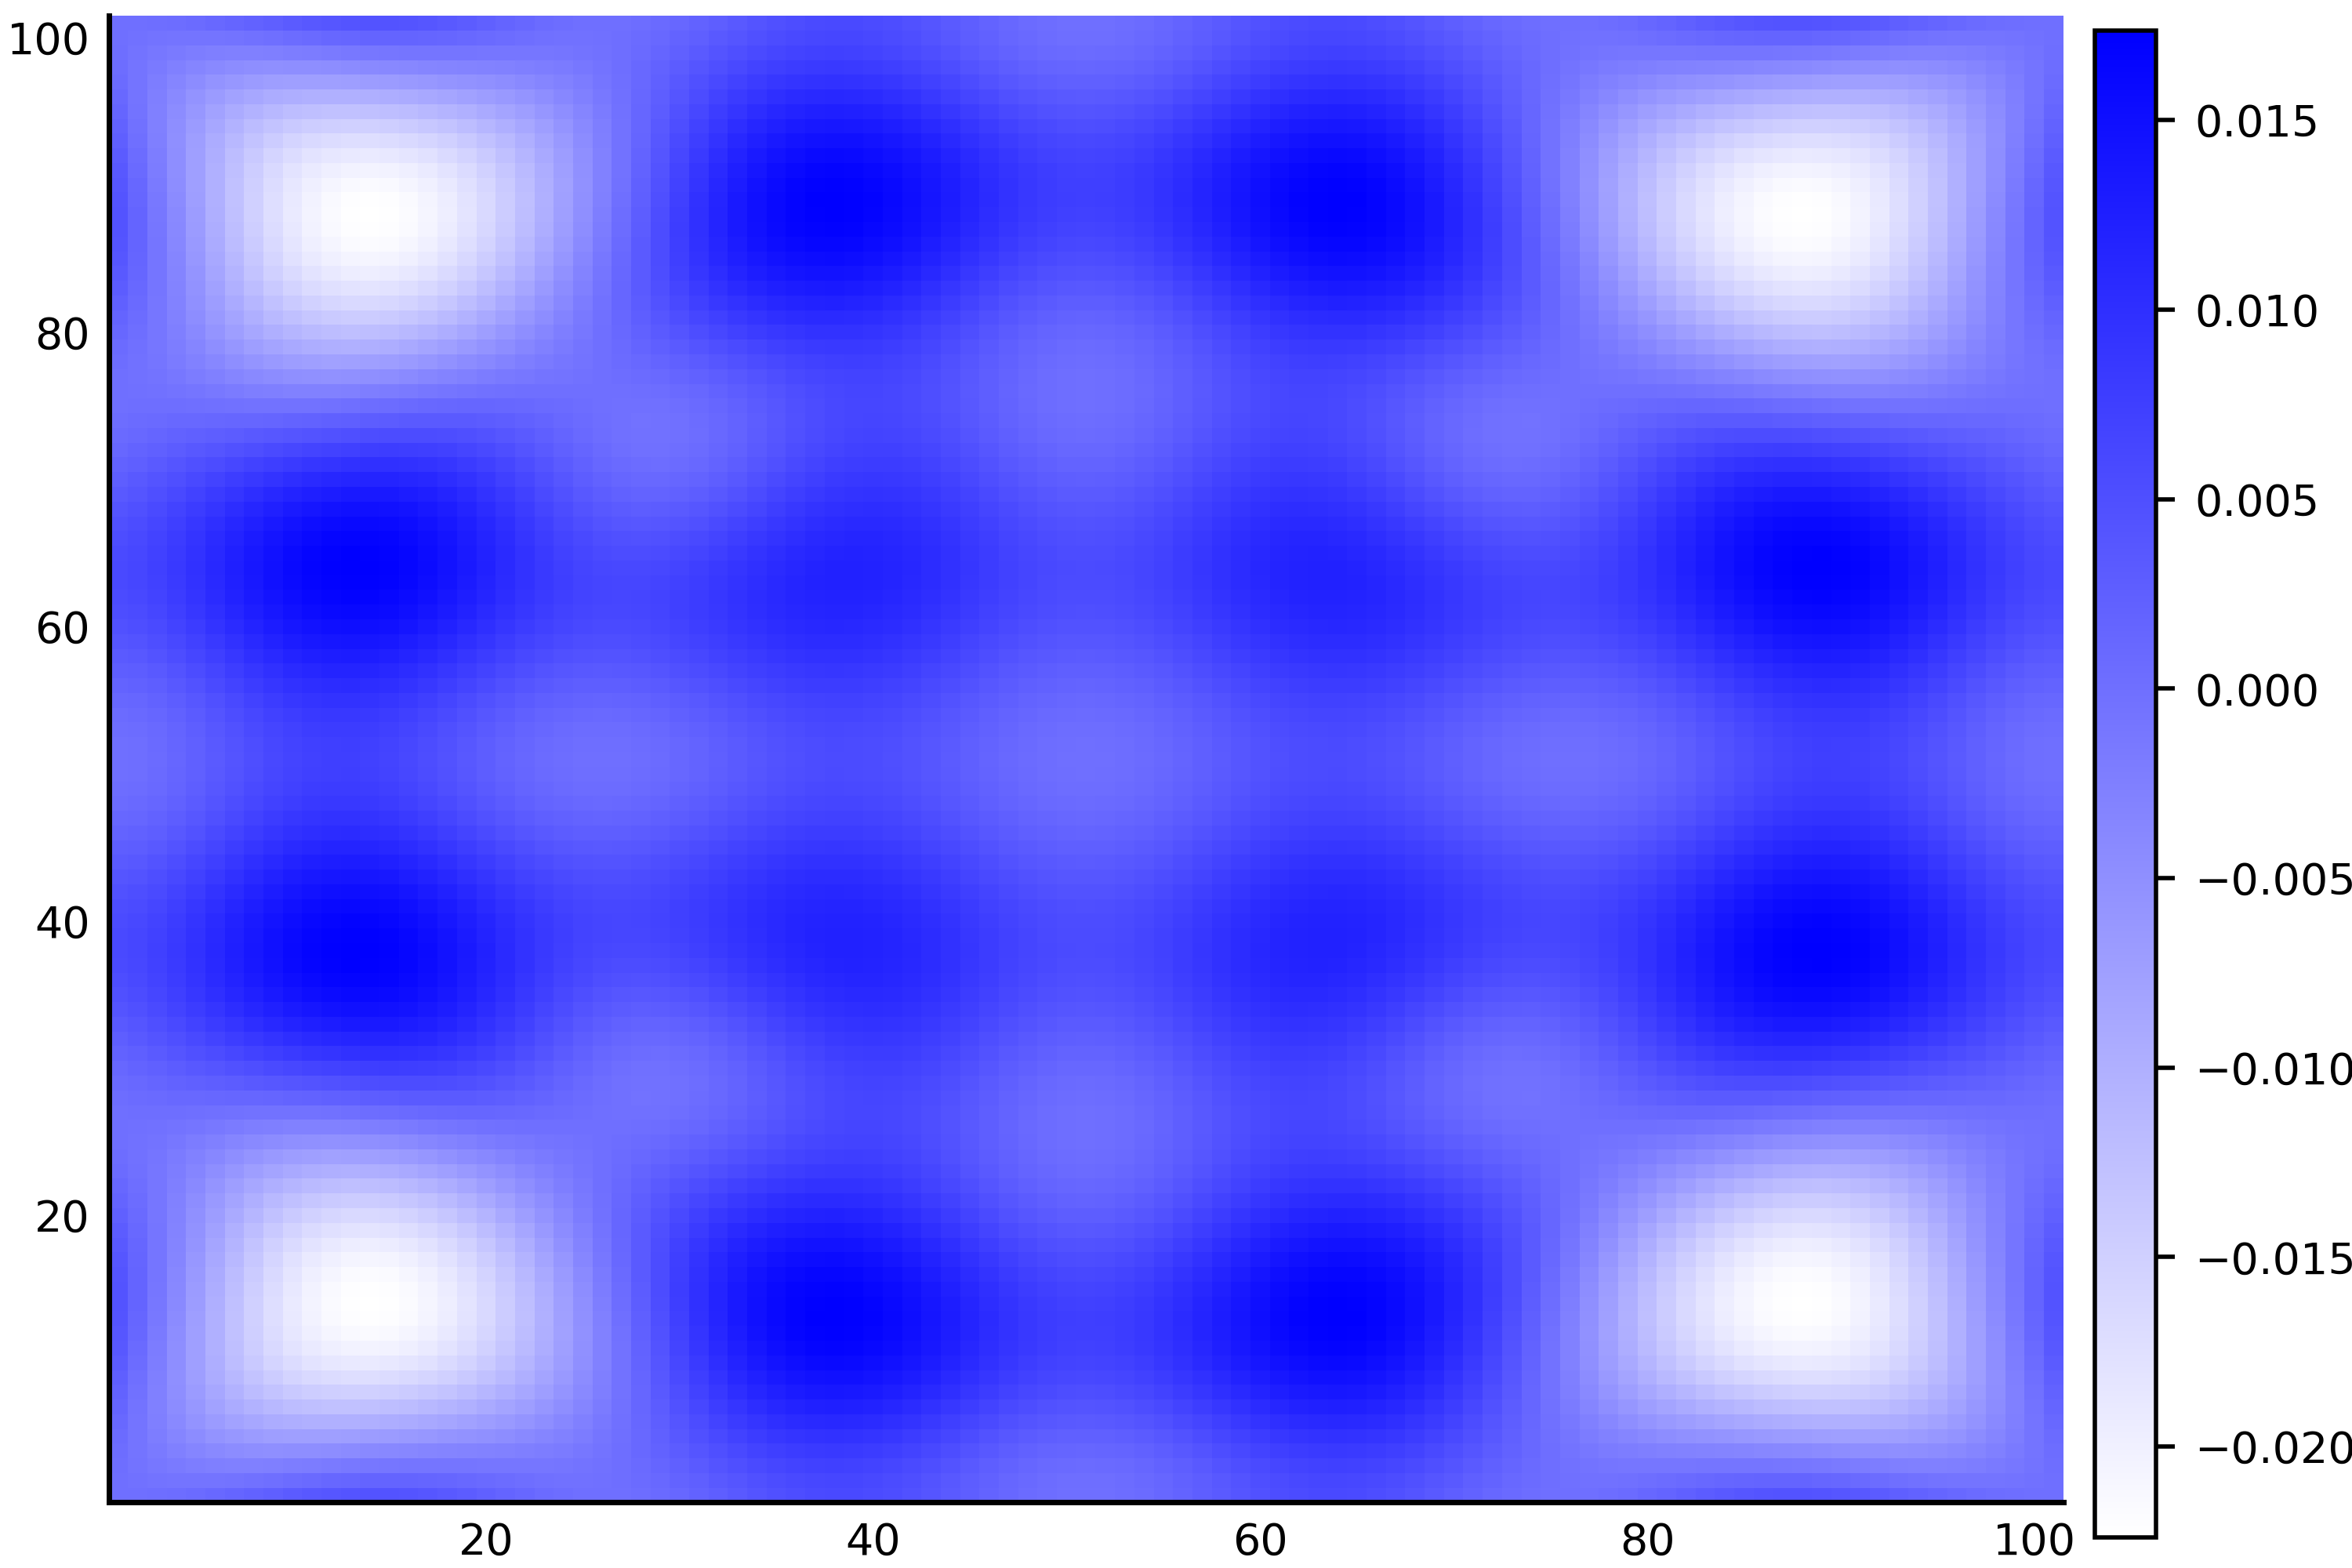
\includegraphics[scale=0.2]{figures/heatmaps/variance-der-25.png}} \\
    \hline
    \centering \textbf{Nonstationary smoothness} &
      \parbox[c]{.18\textwidth}{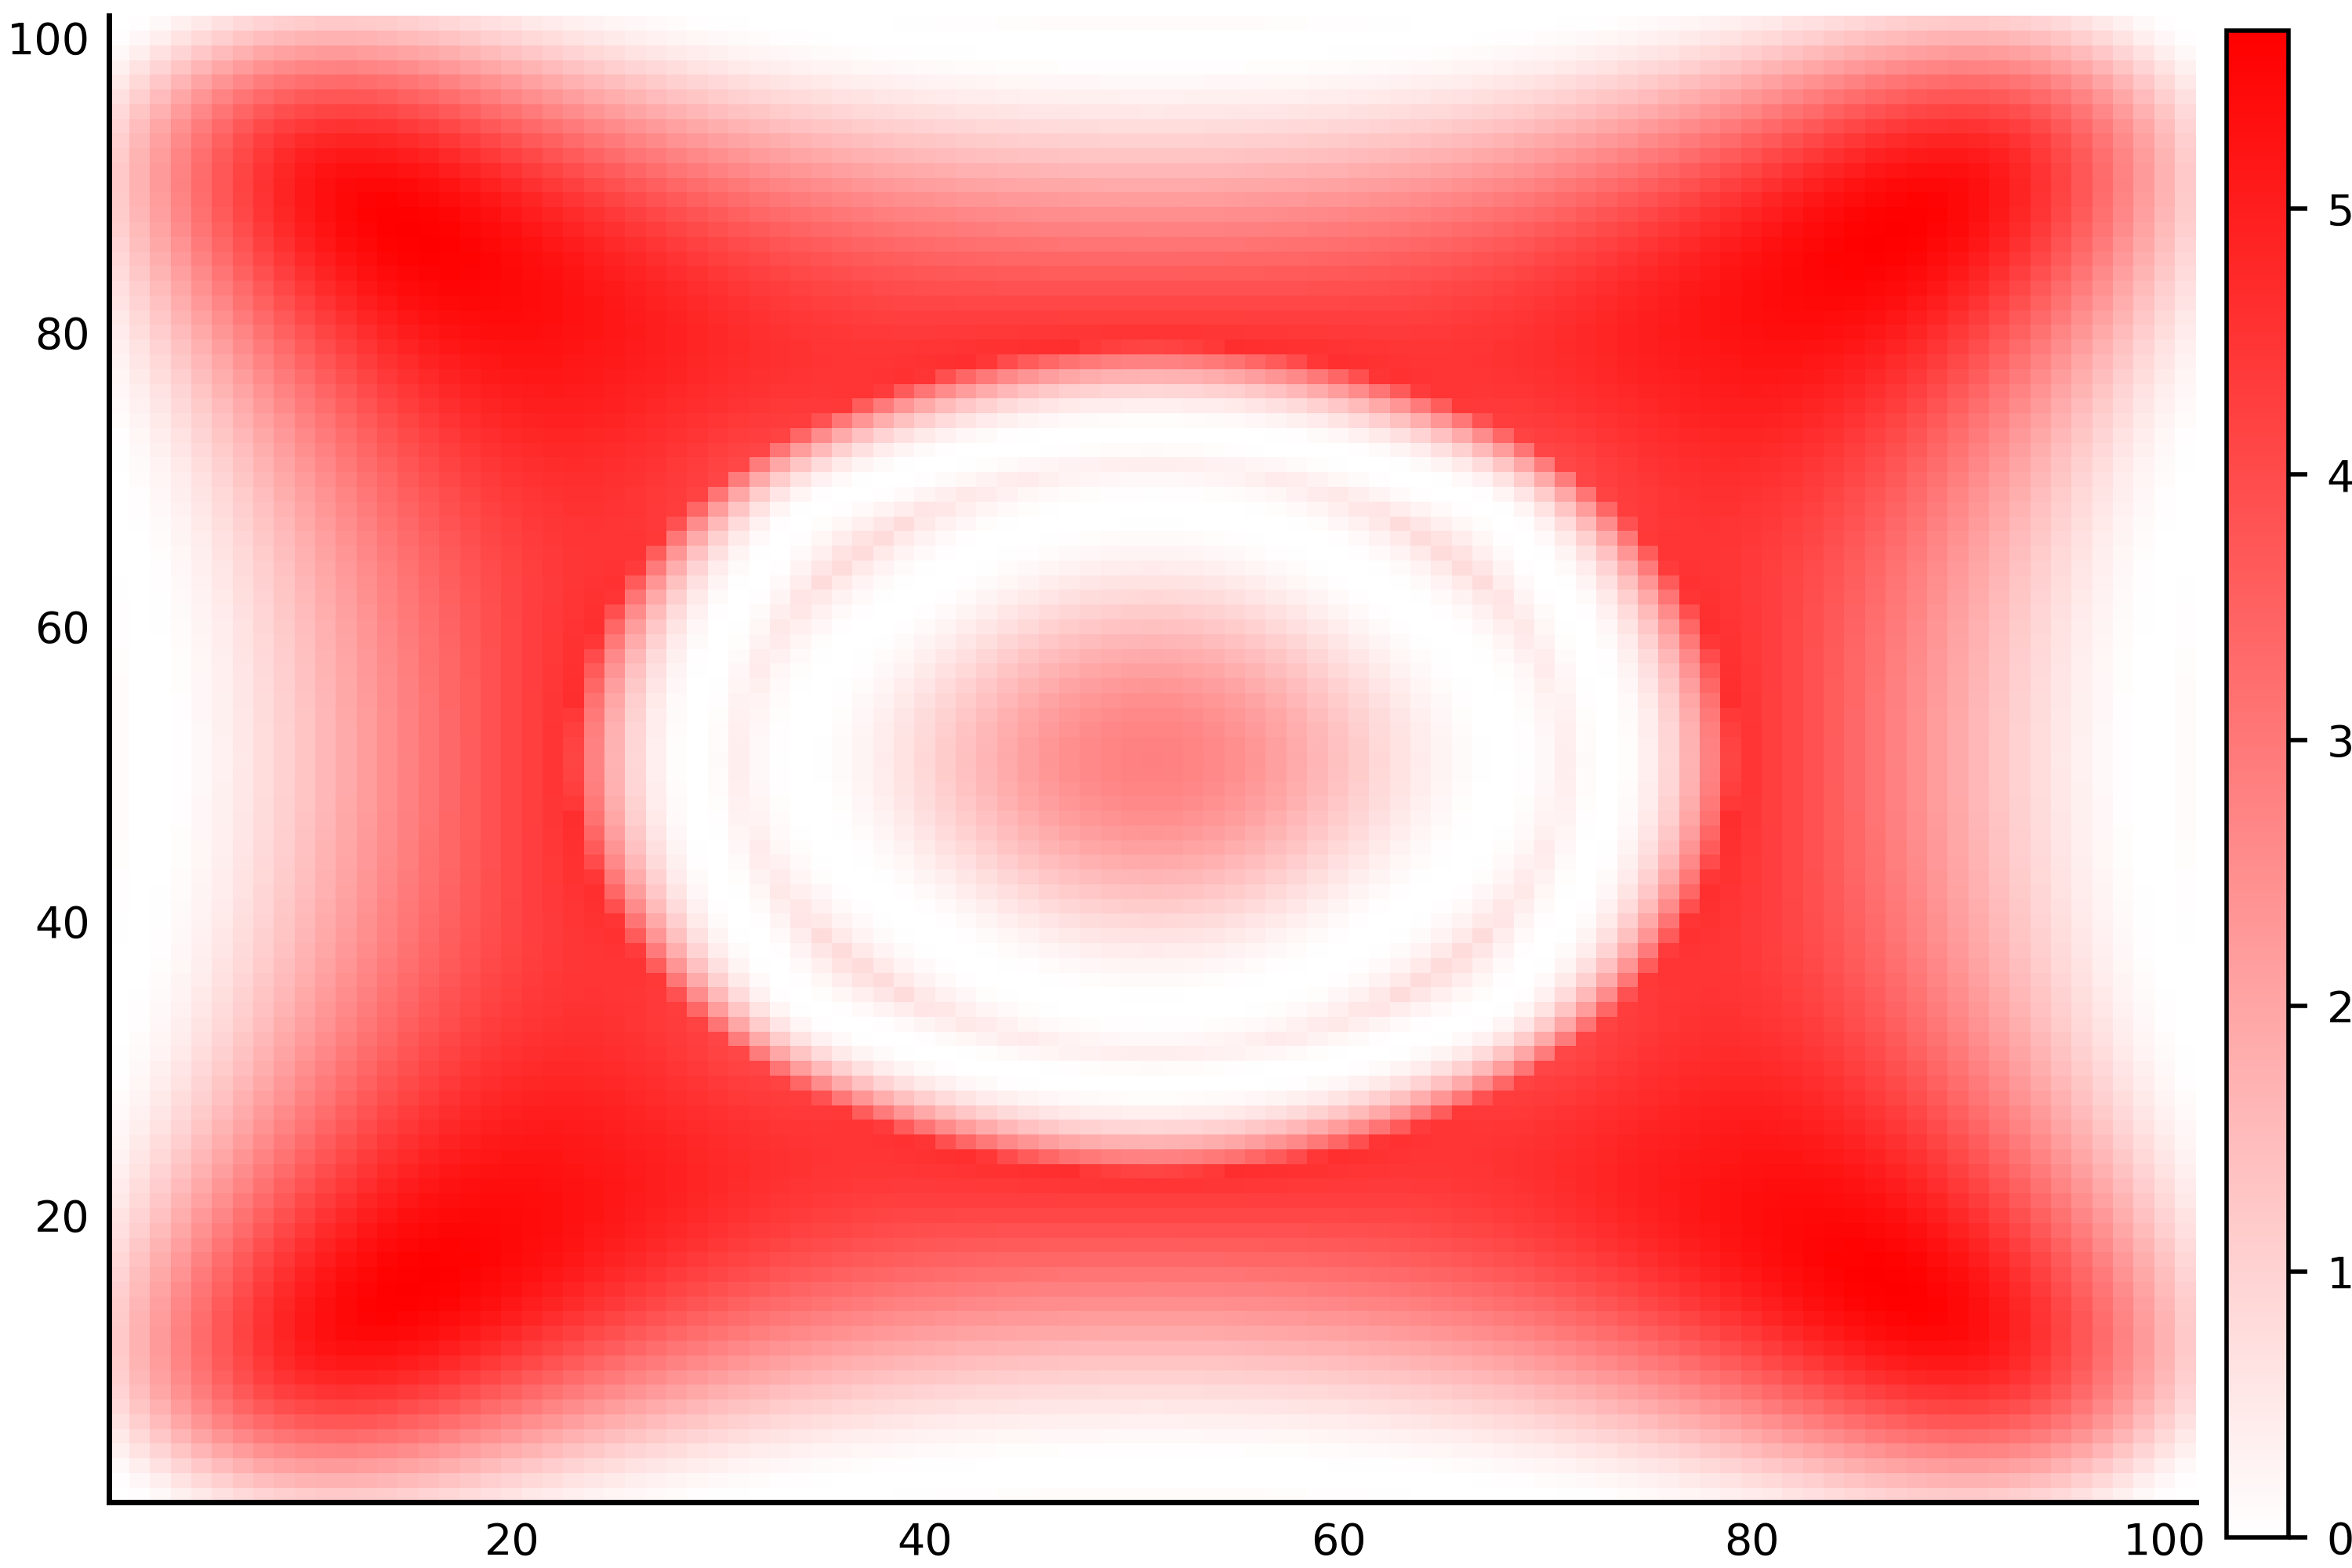
\includegraphics[scale=0.2]{figures/heatmaps/error-smoothness-16.png}} &
      \parbox[c]{.18\textwidth}{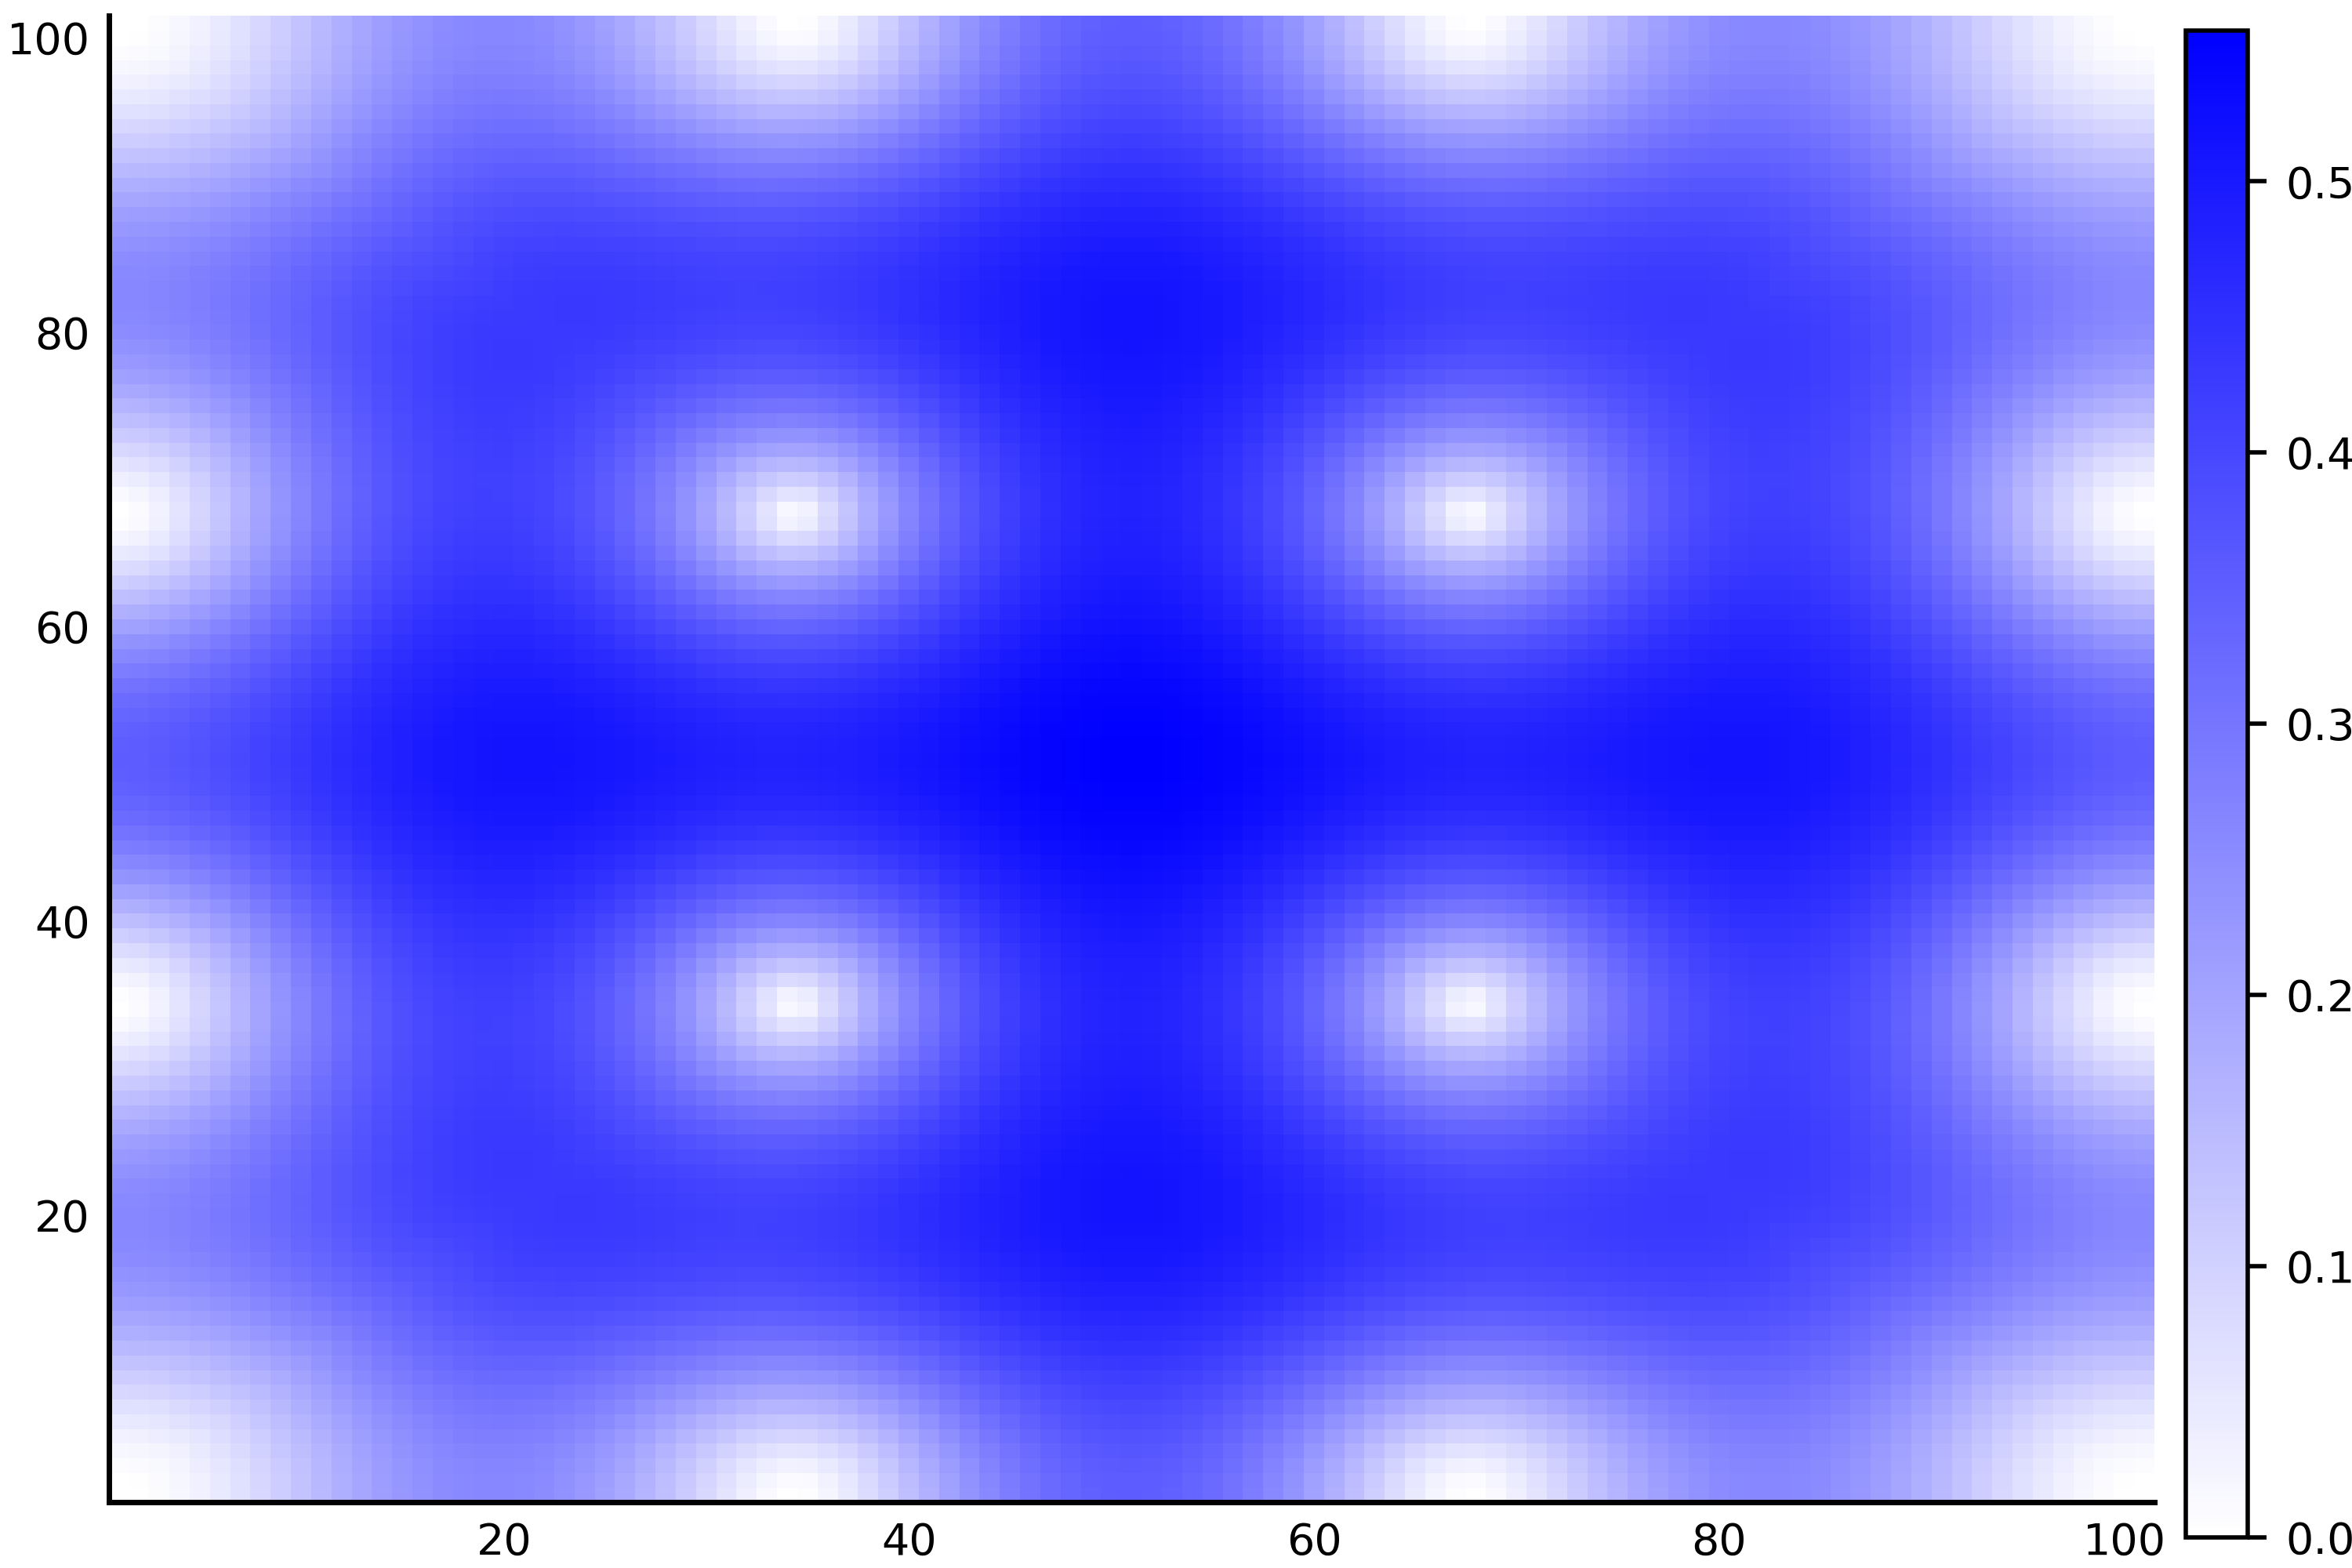
\includegraphics[scale=0.2]{figures/heatmaps/variance-smoothness-16.png}} &
      \parbox[c]{.18\textwidth}{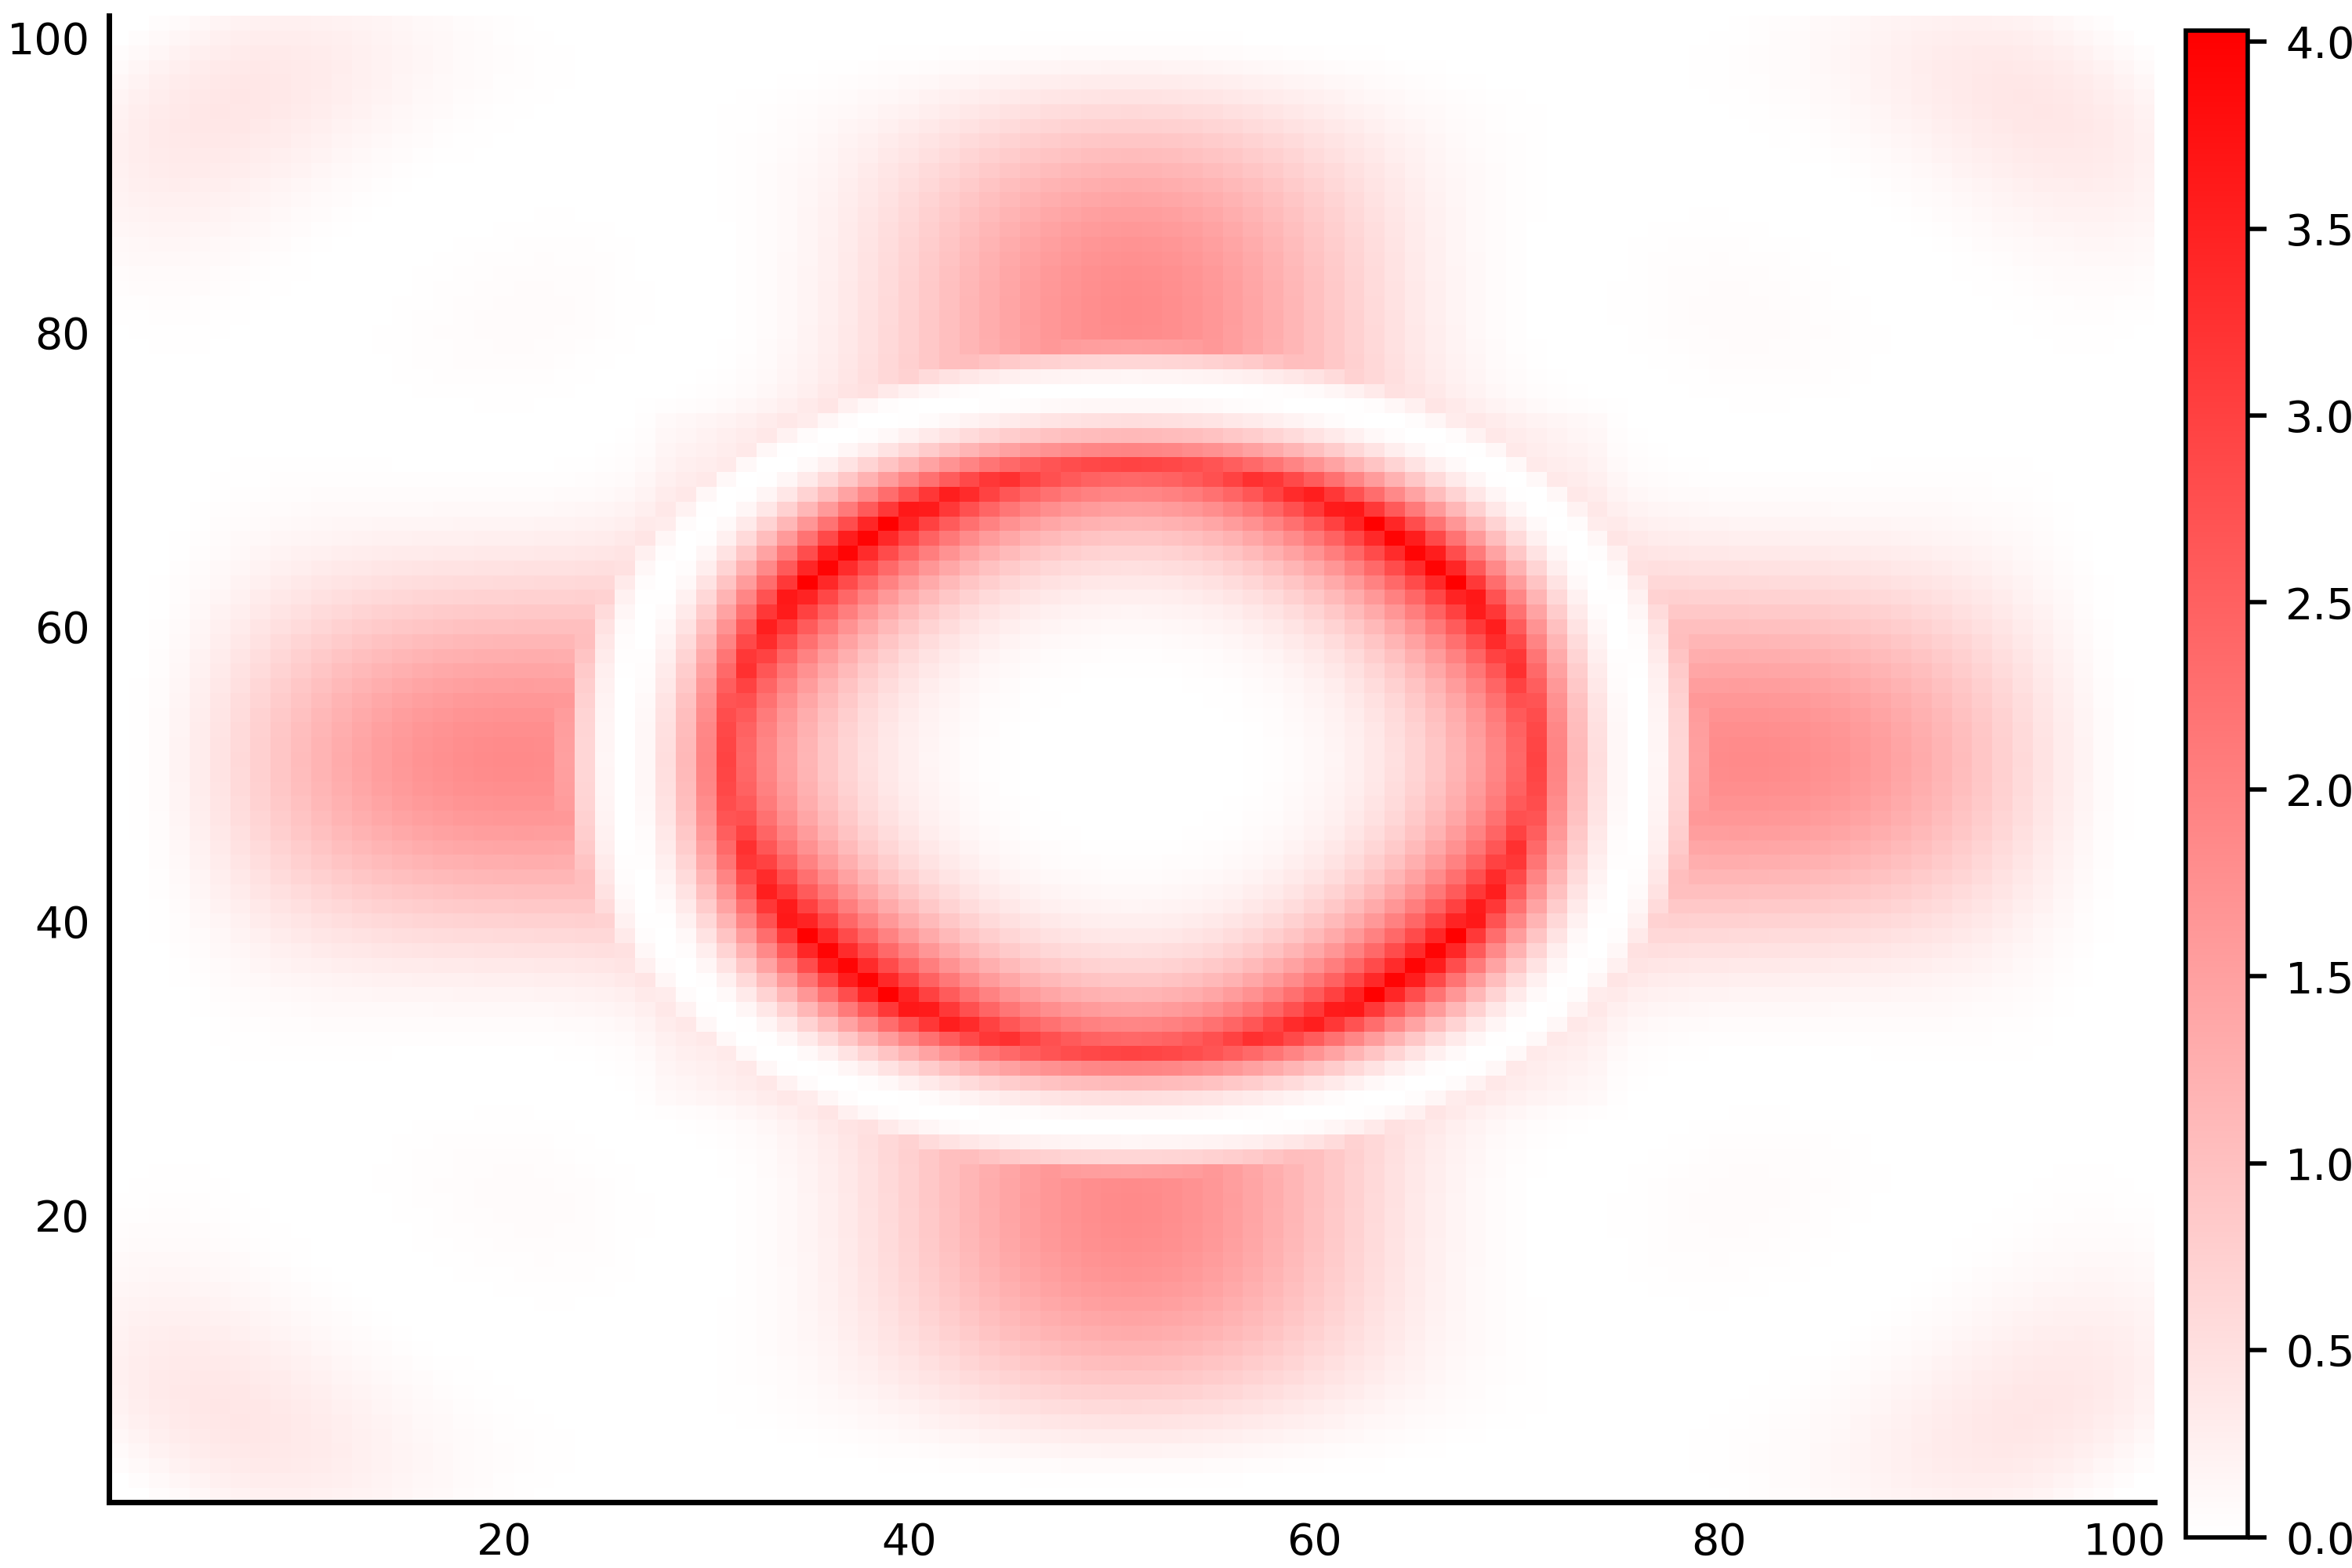
\includegraphics[scale=0.2]{figures/heatmaps/error-smoothness-25.png}} &
      \parbox[c]{.18\textwidth}{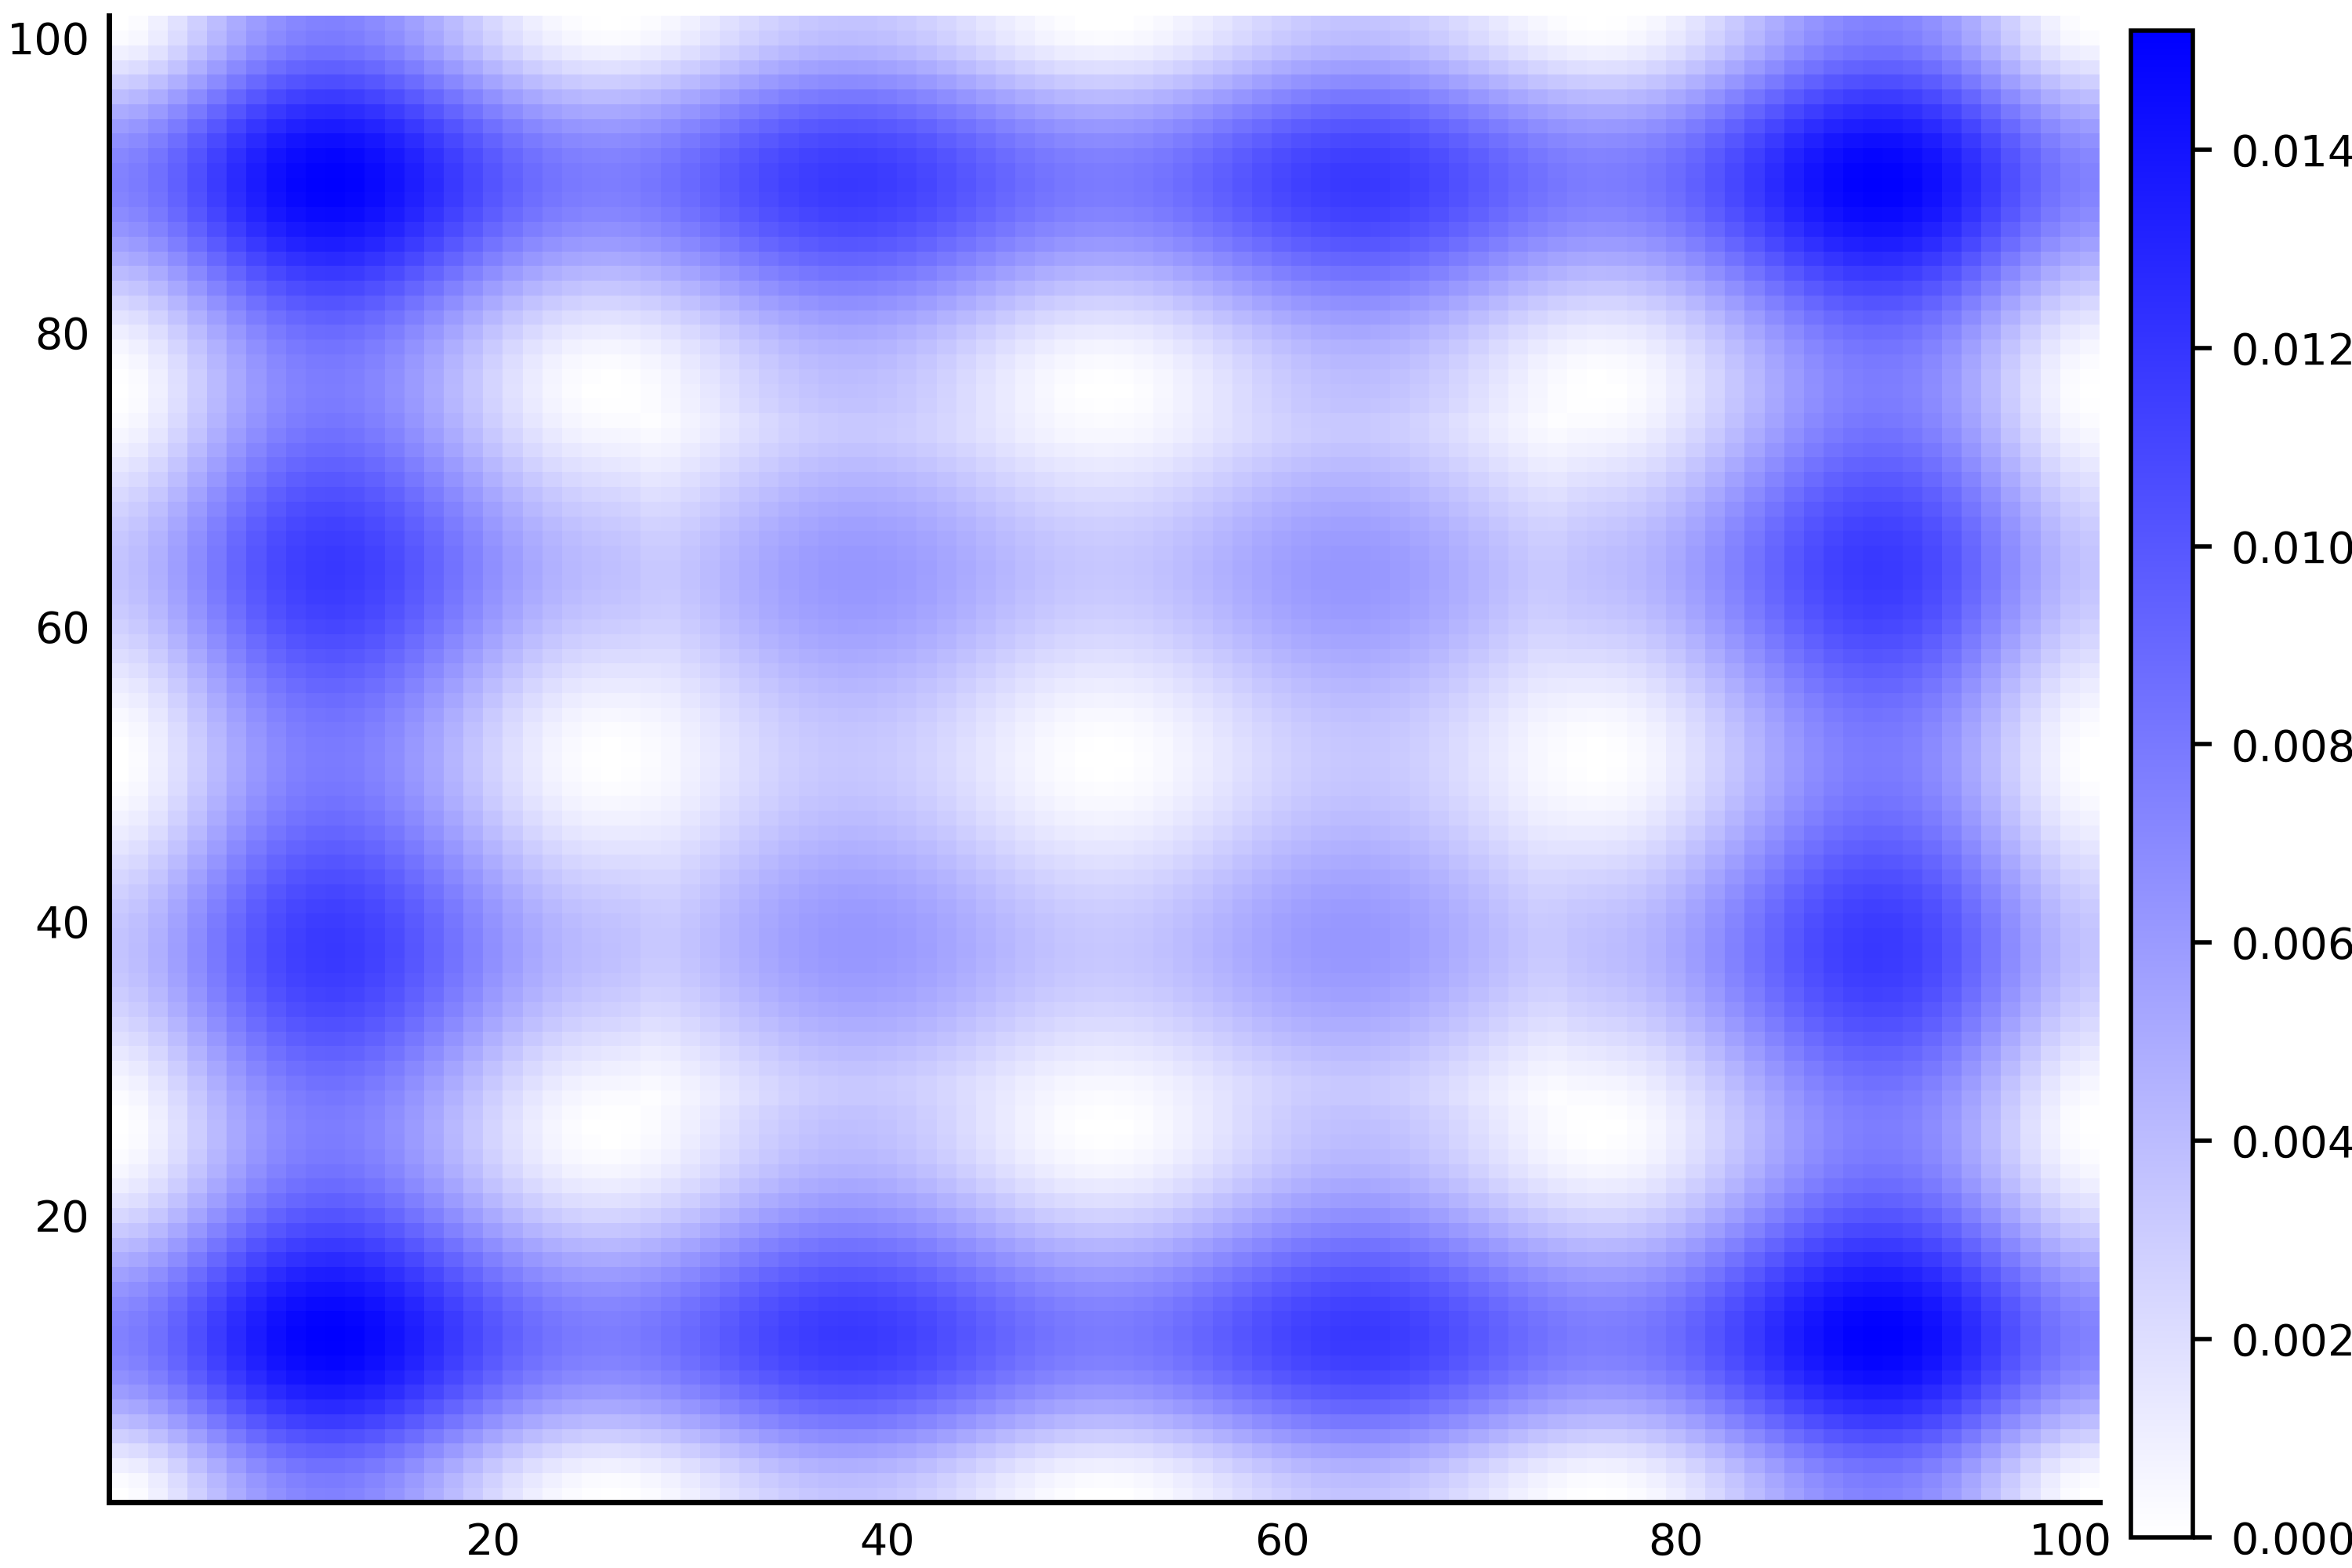
\includegraphics[scale=0.2]{figures/heatmaps/variance-smoothness-25.png}} \\
    \hline
    \centering \textbf{Mixture of GPs} &
      \parbox[c]{.18\textwidth}{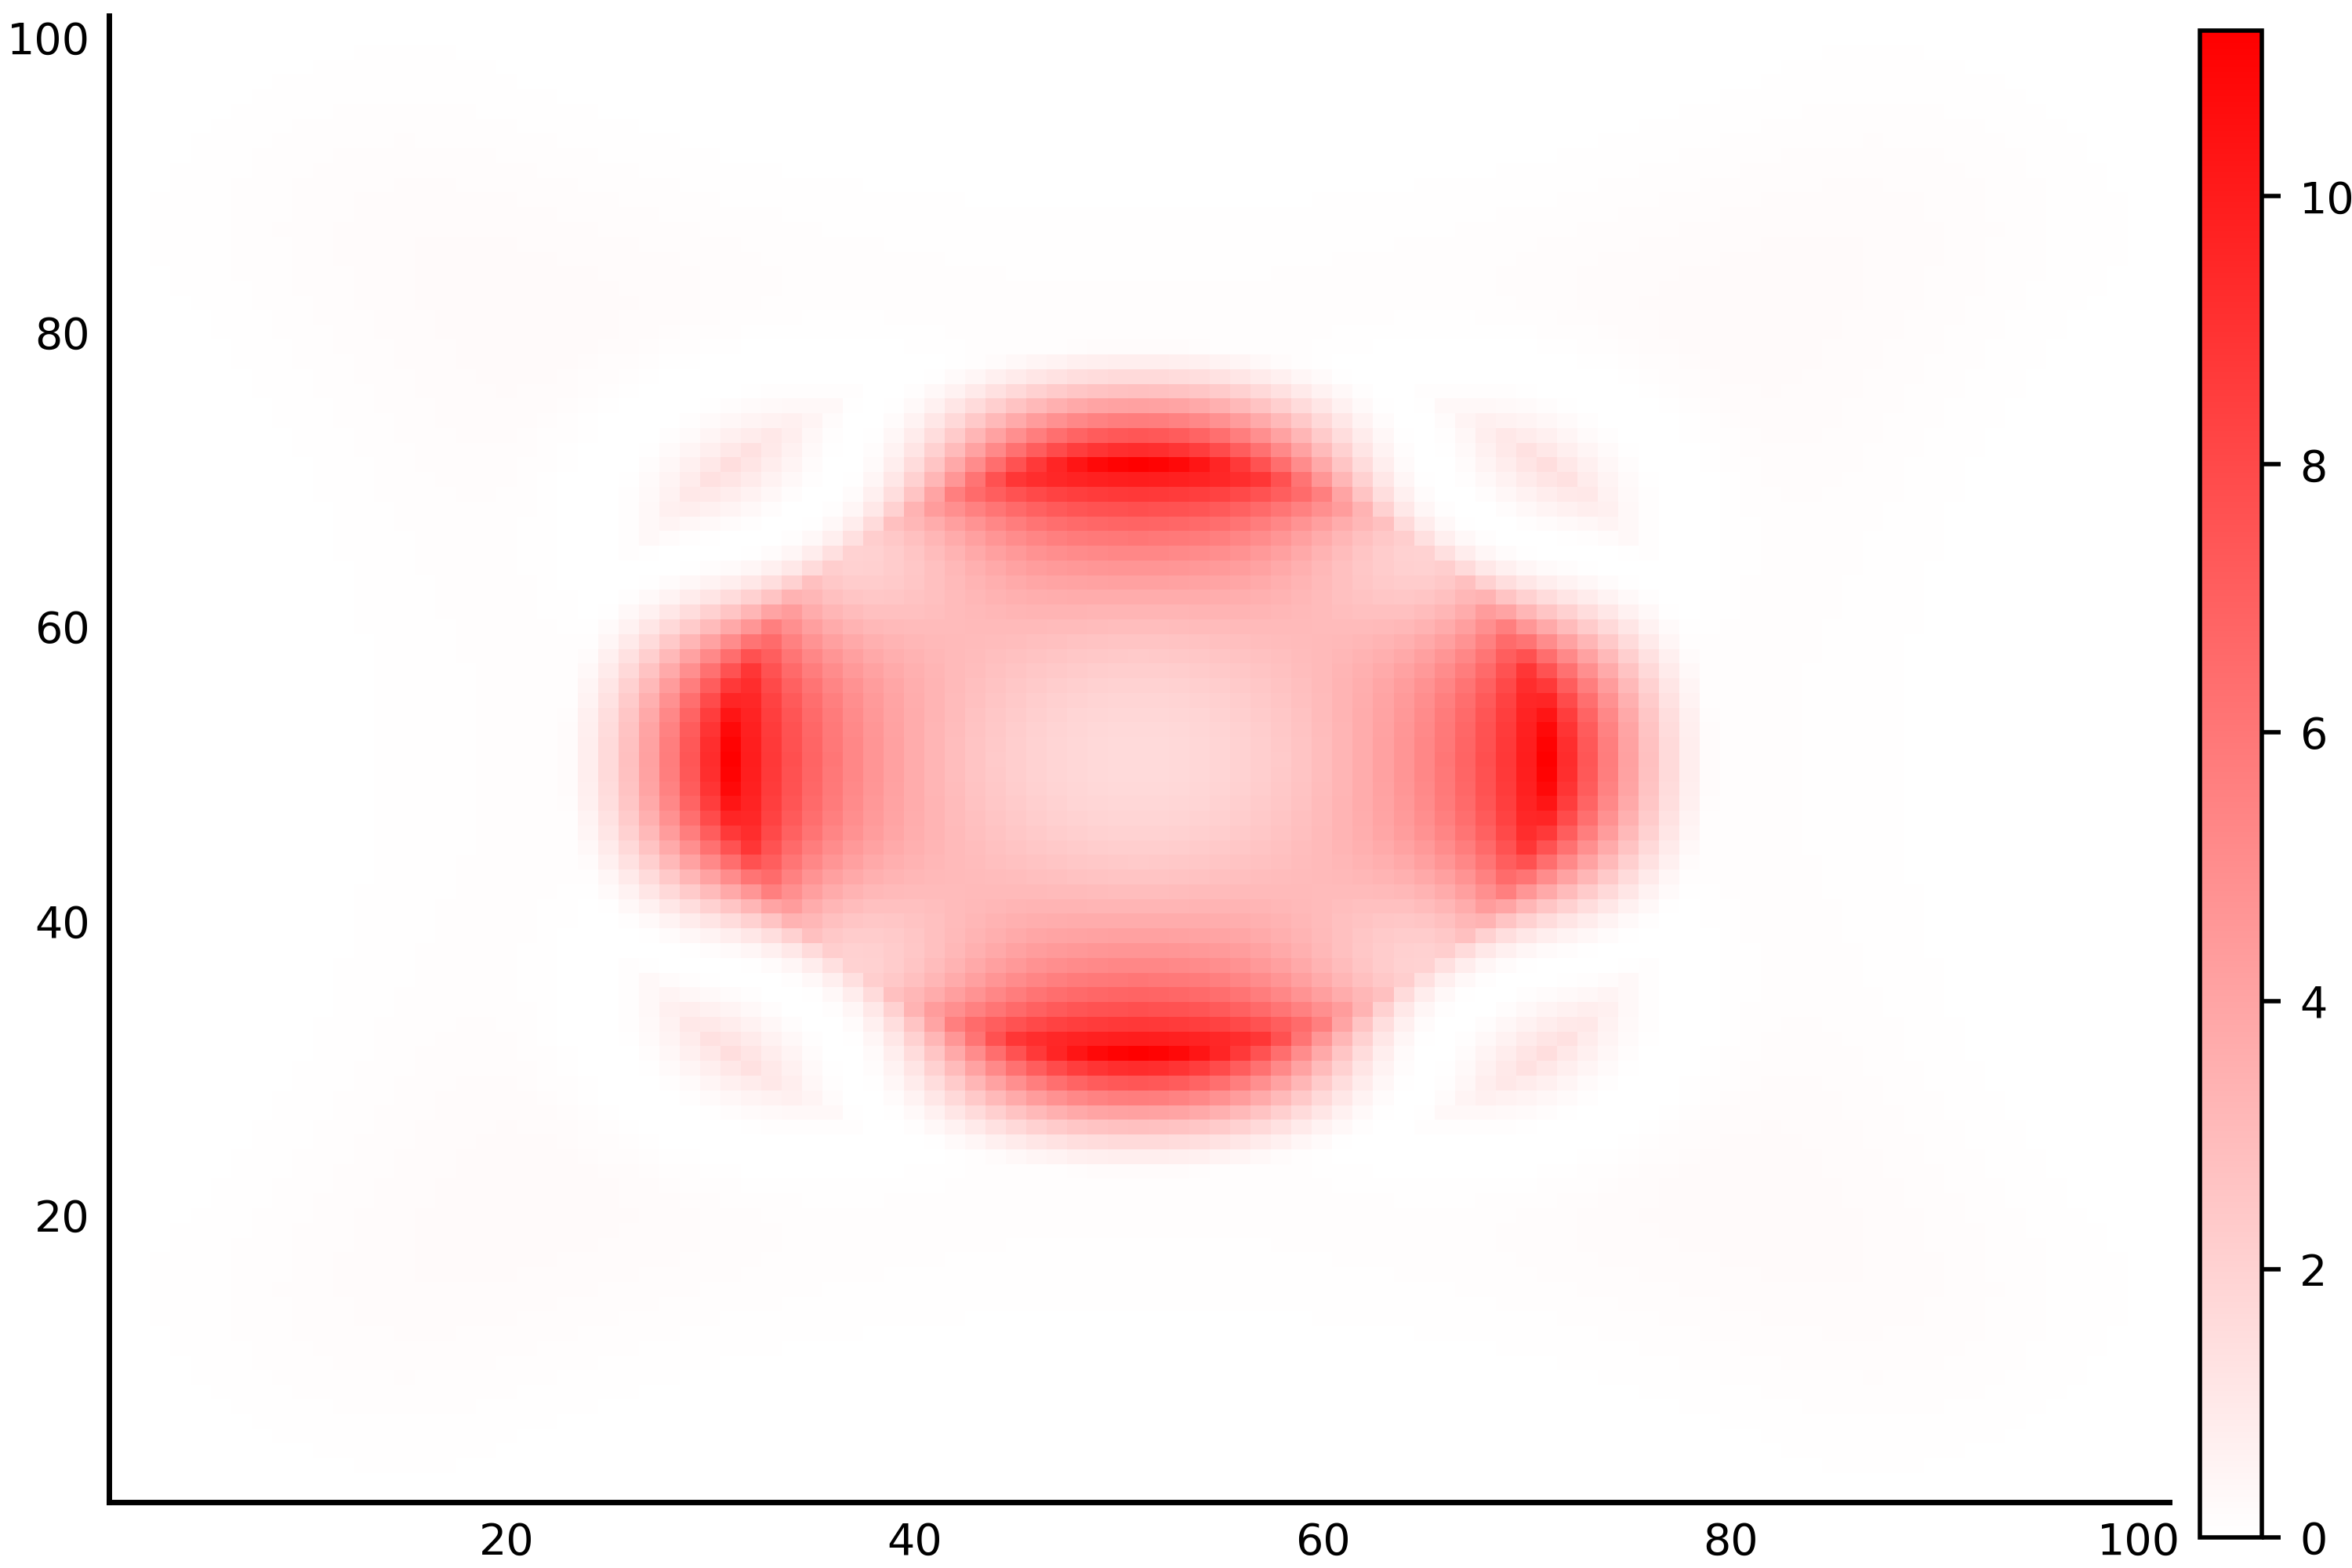
\includegraphics[scale=0.2]{figures/heatmaps/error-mixture-16.png}} &
      \parbox[c]{.18\textwidth}{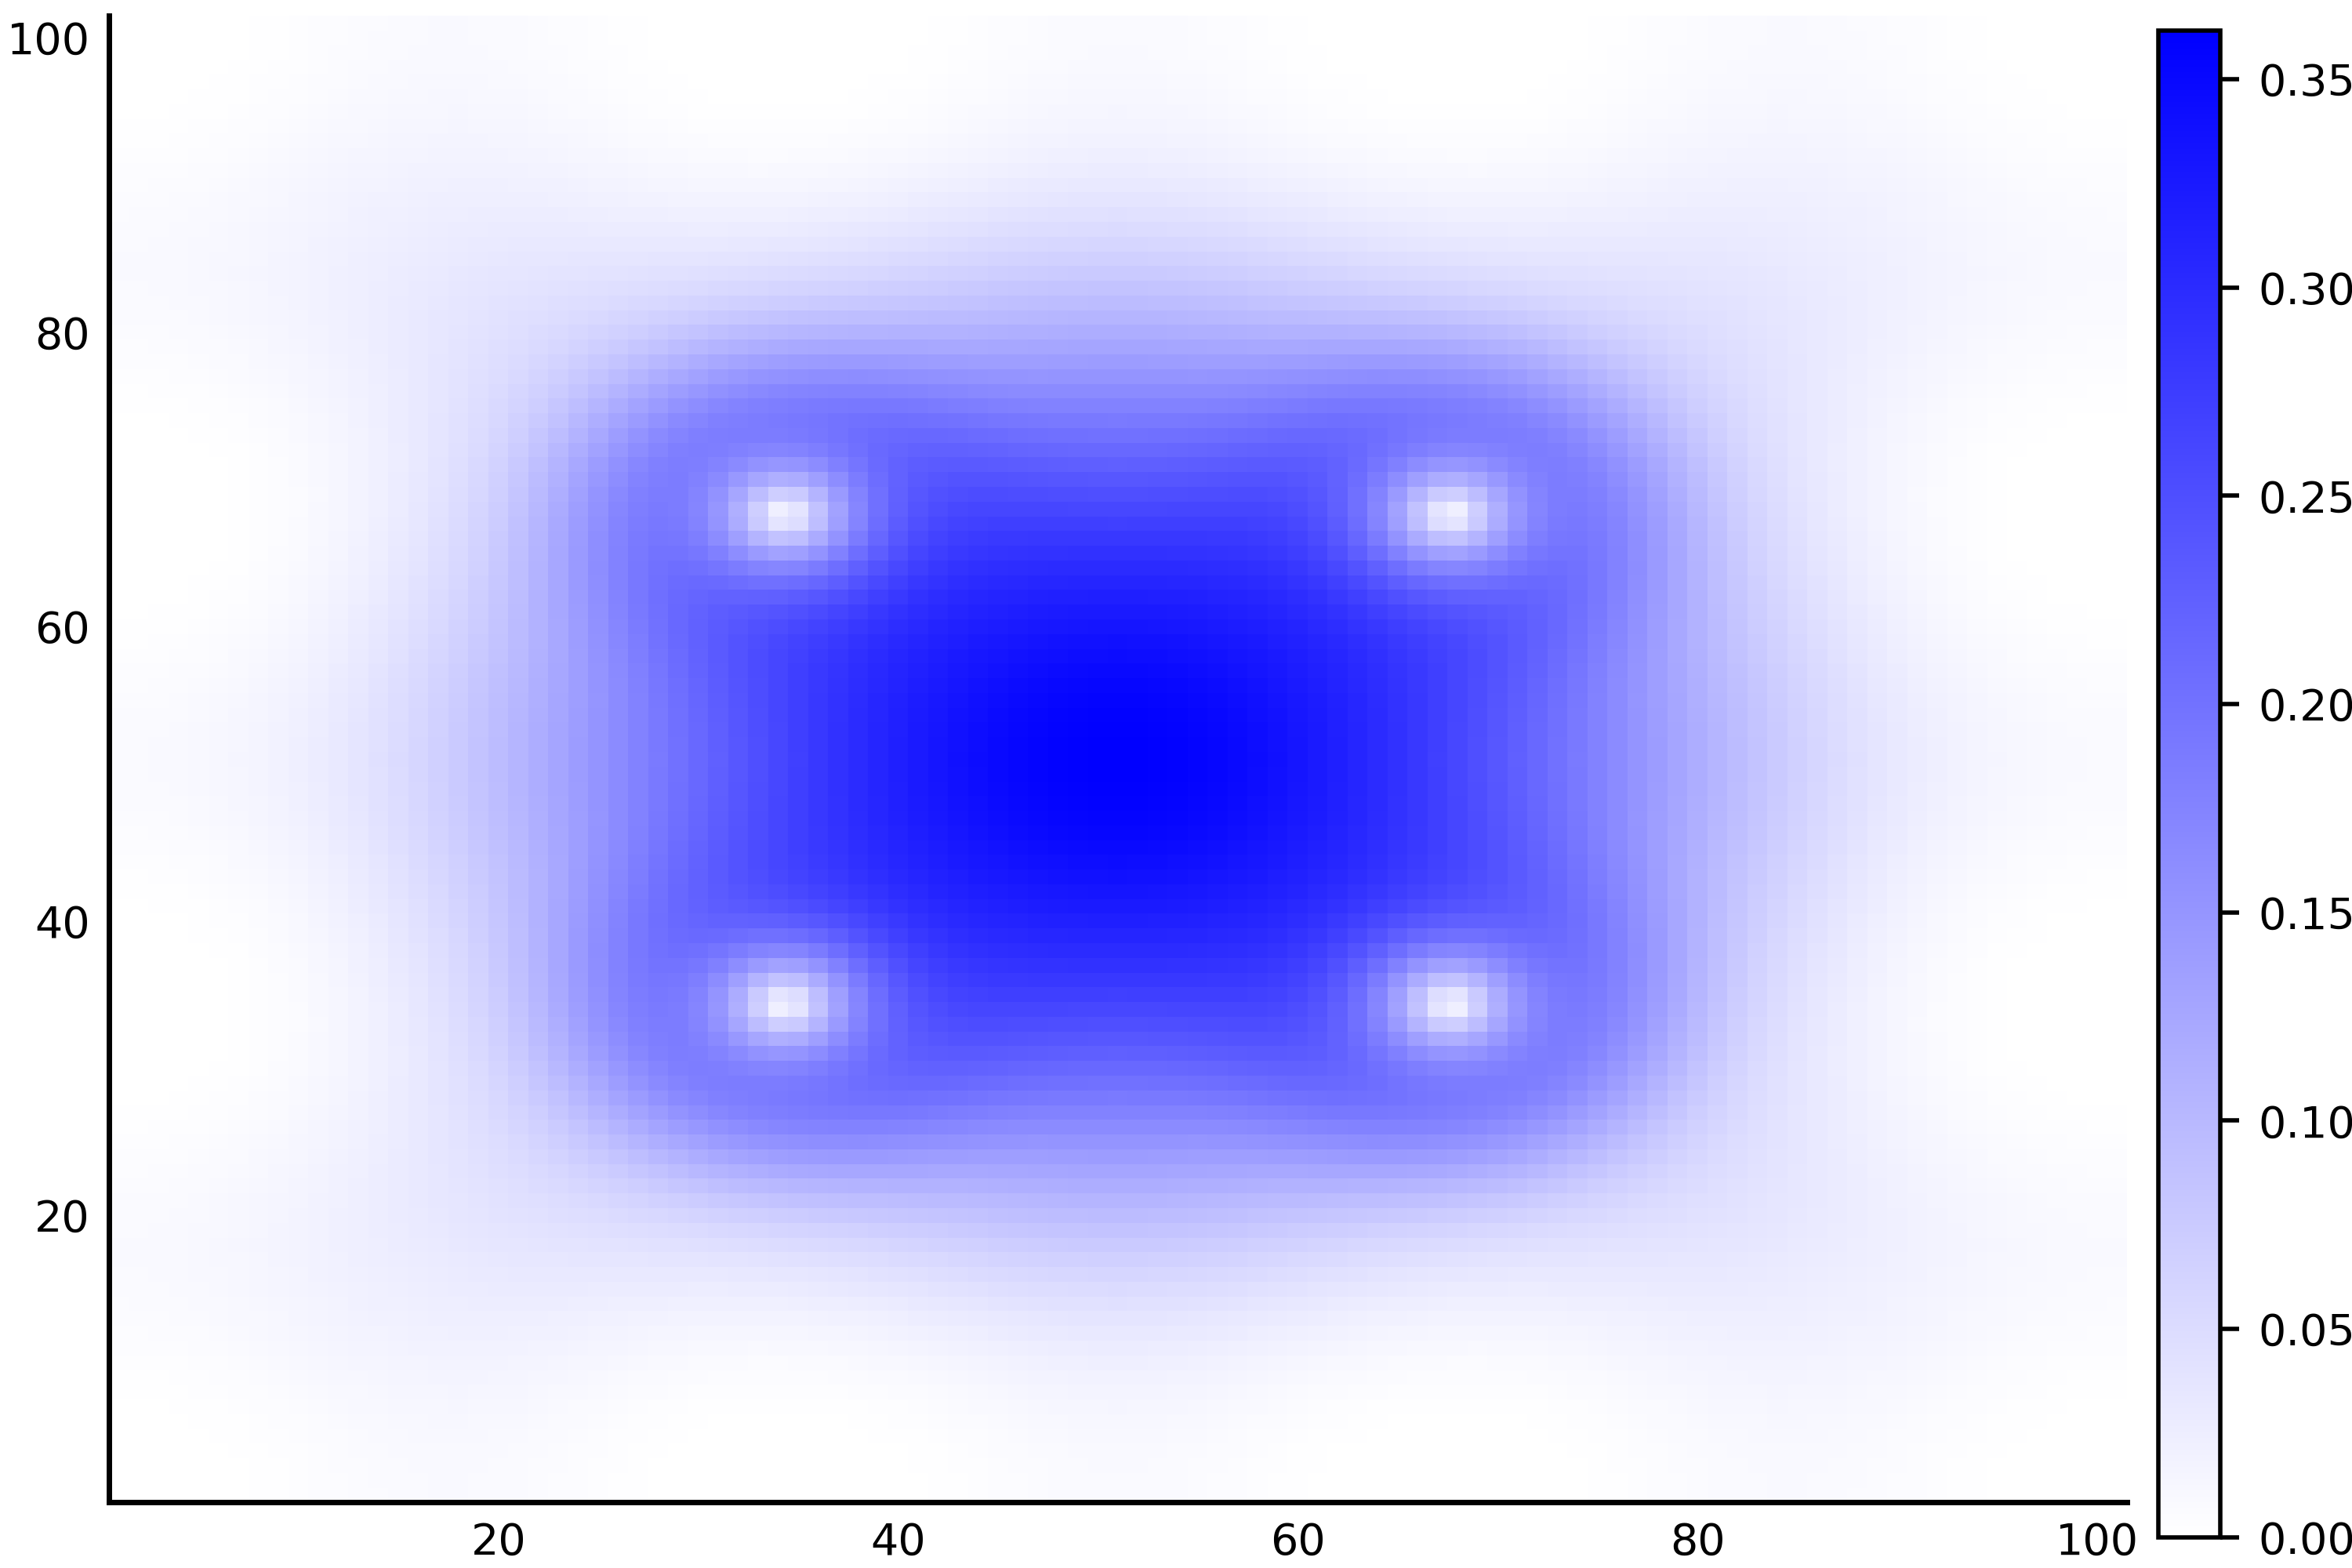
\includegraphics[scale=0.2]{figures/heatmaps/variance-mixture-16.png}} &
      \parbox[c]{.18\textwidth}{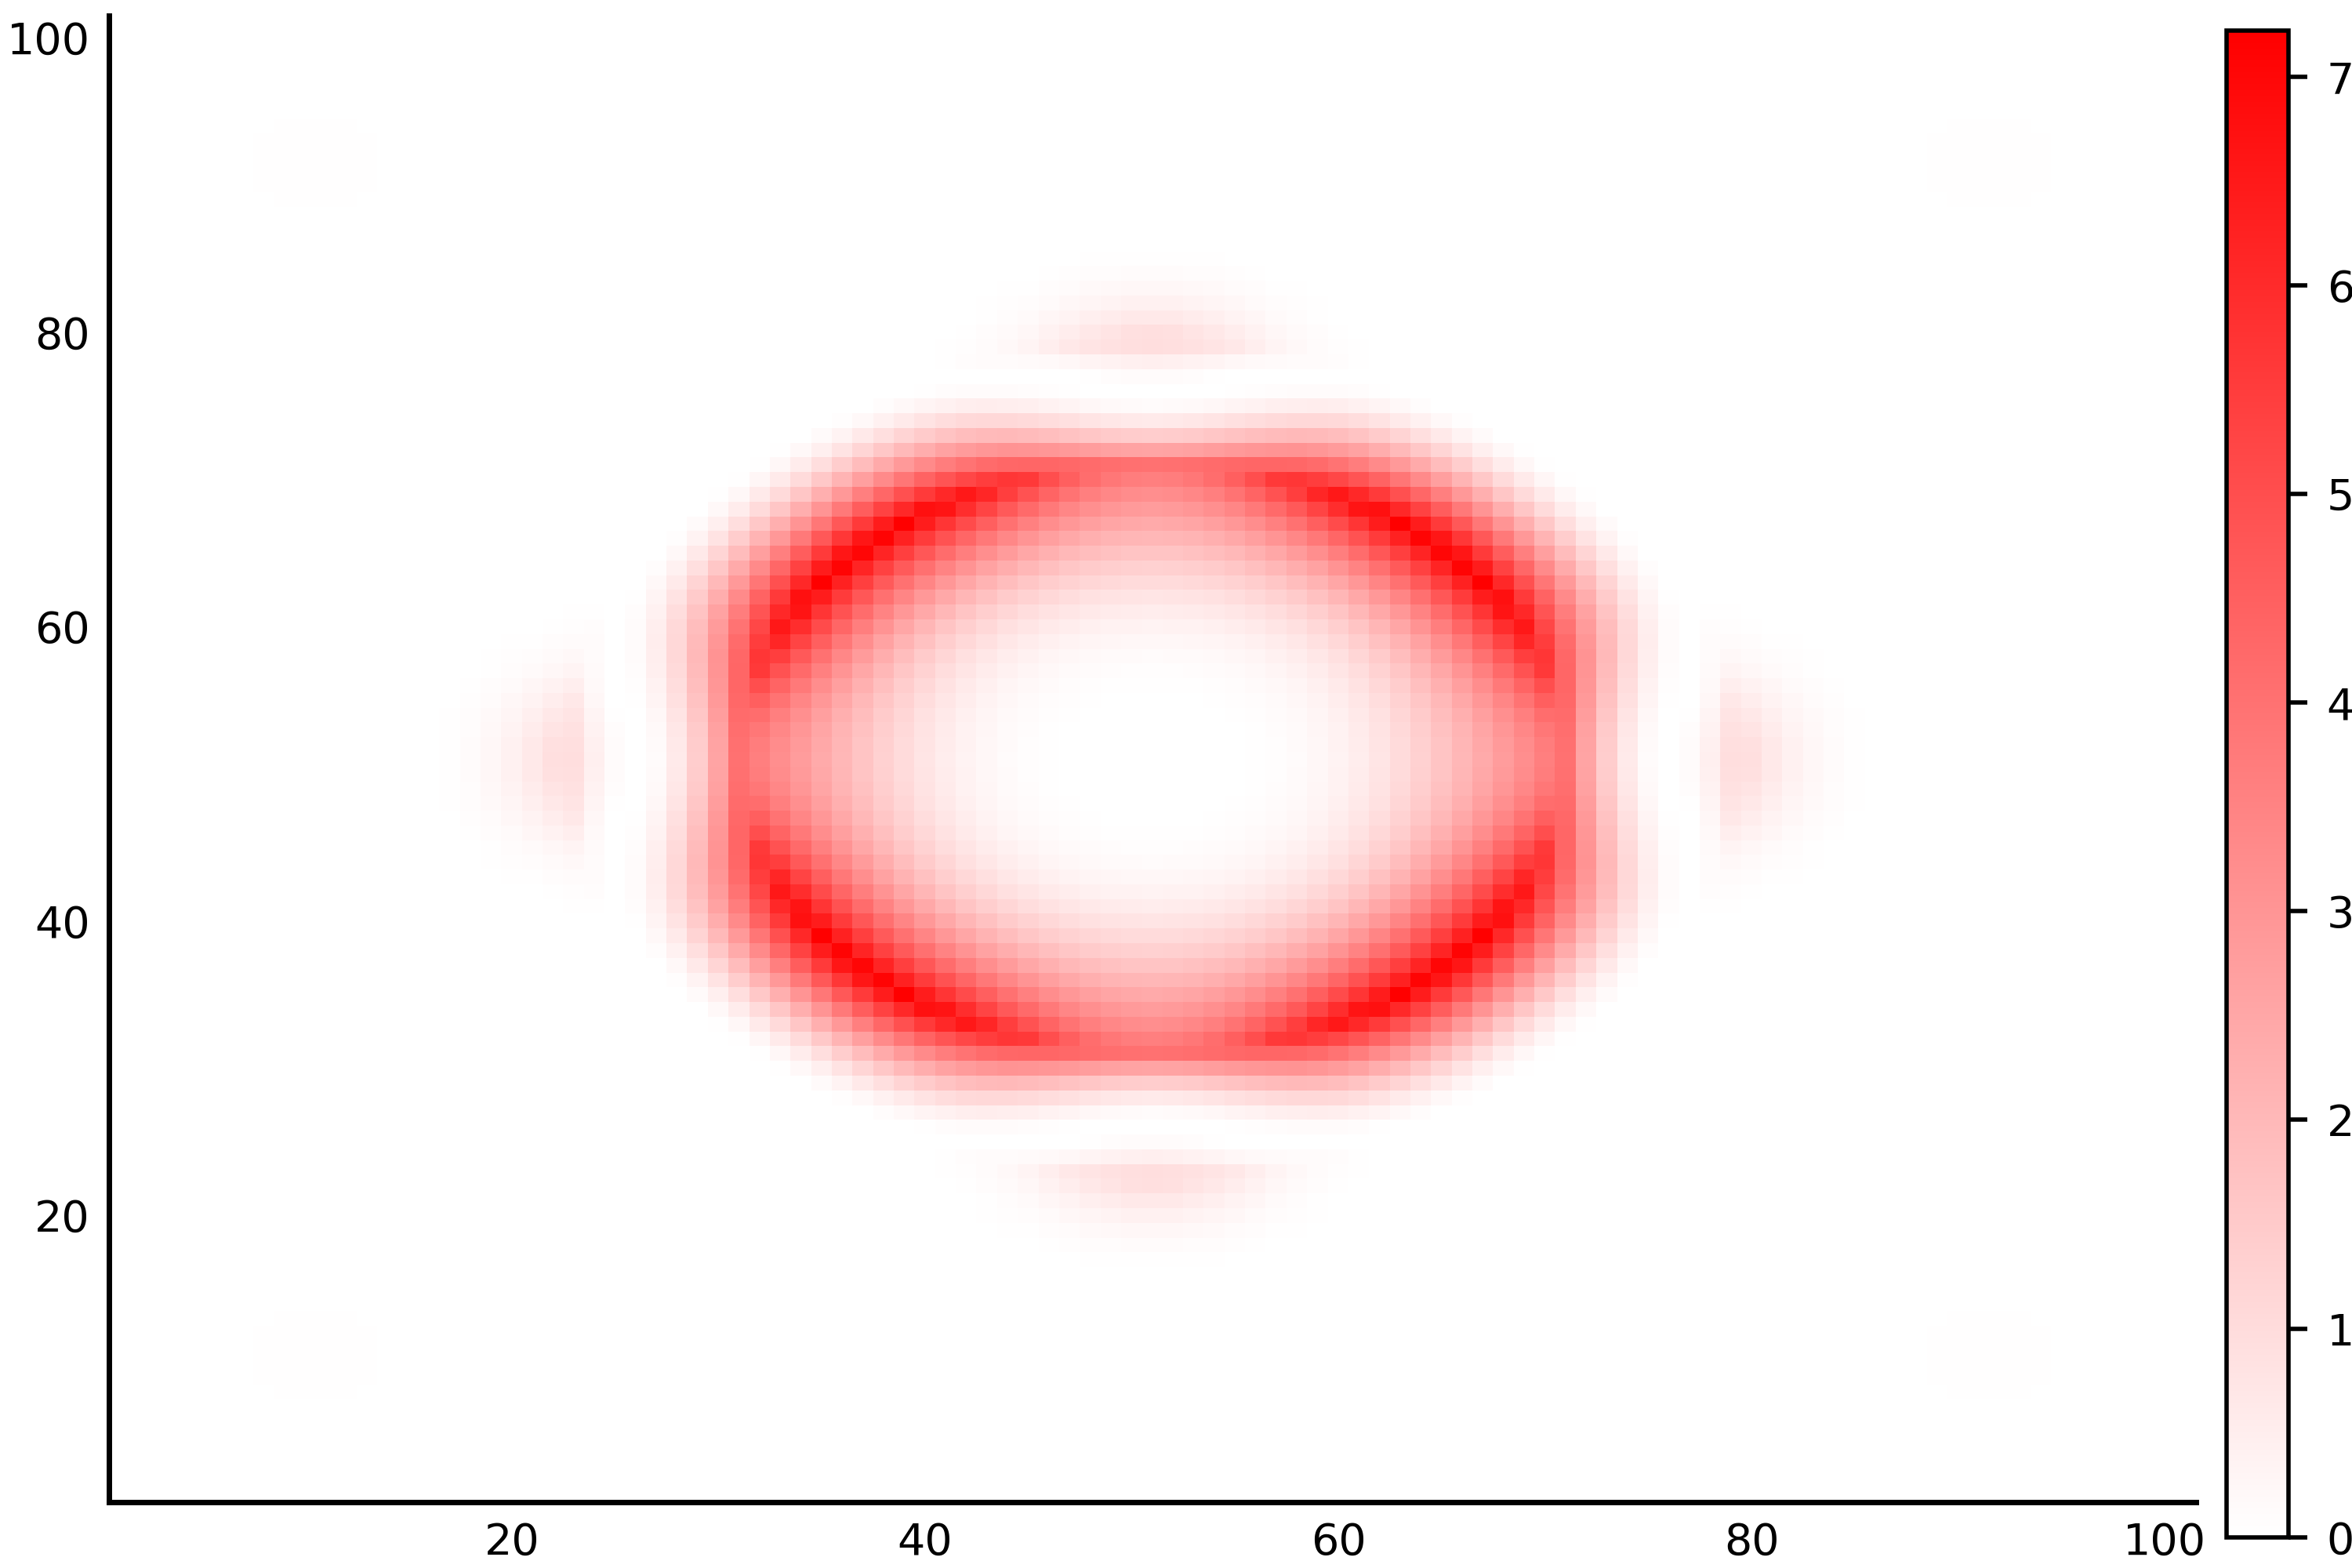
\includegraphics[scale=0.2]{figures/heatmaps/error-mixture-25.png}} &
      \parbox[c]{.18\textwidth}{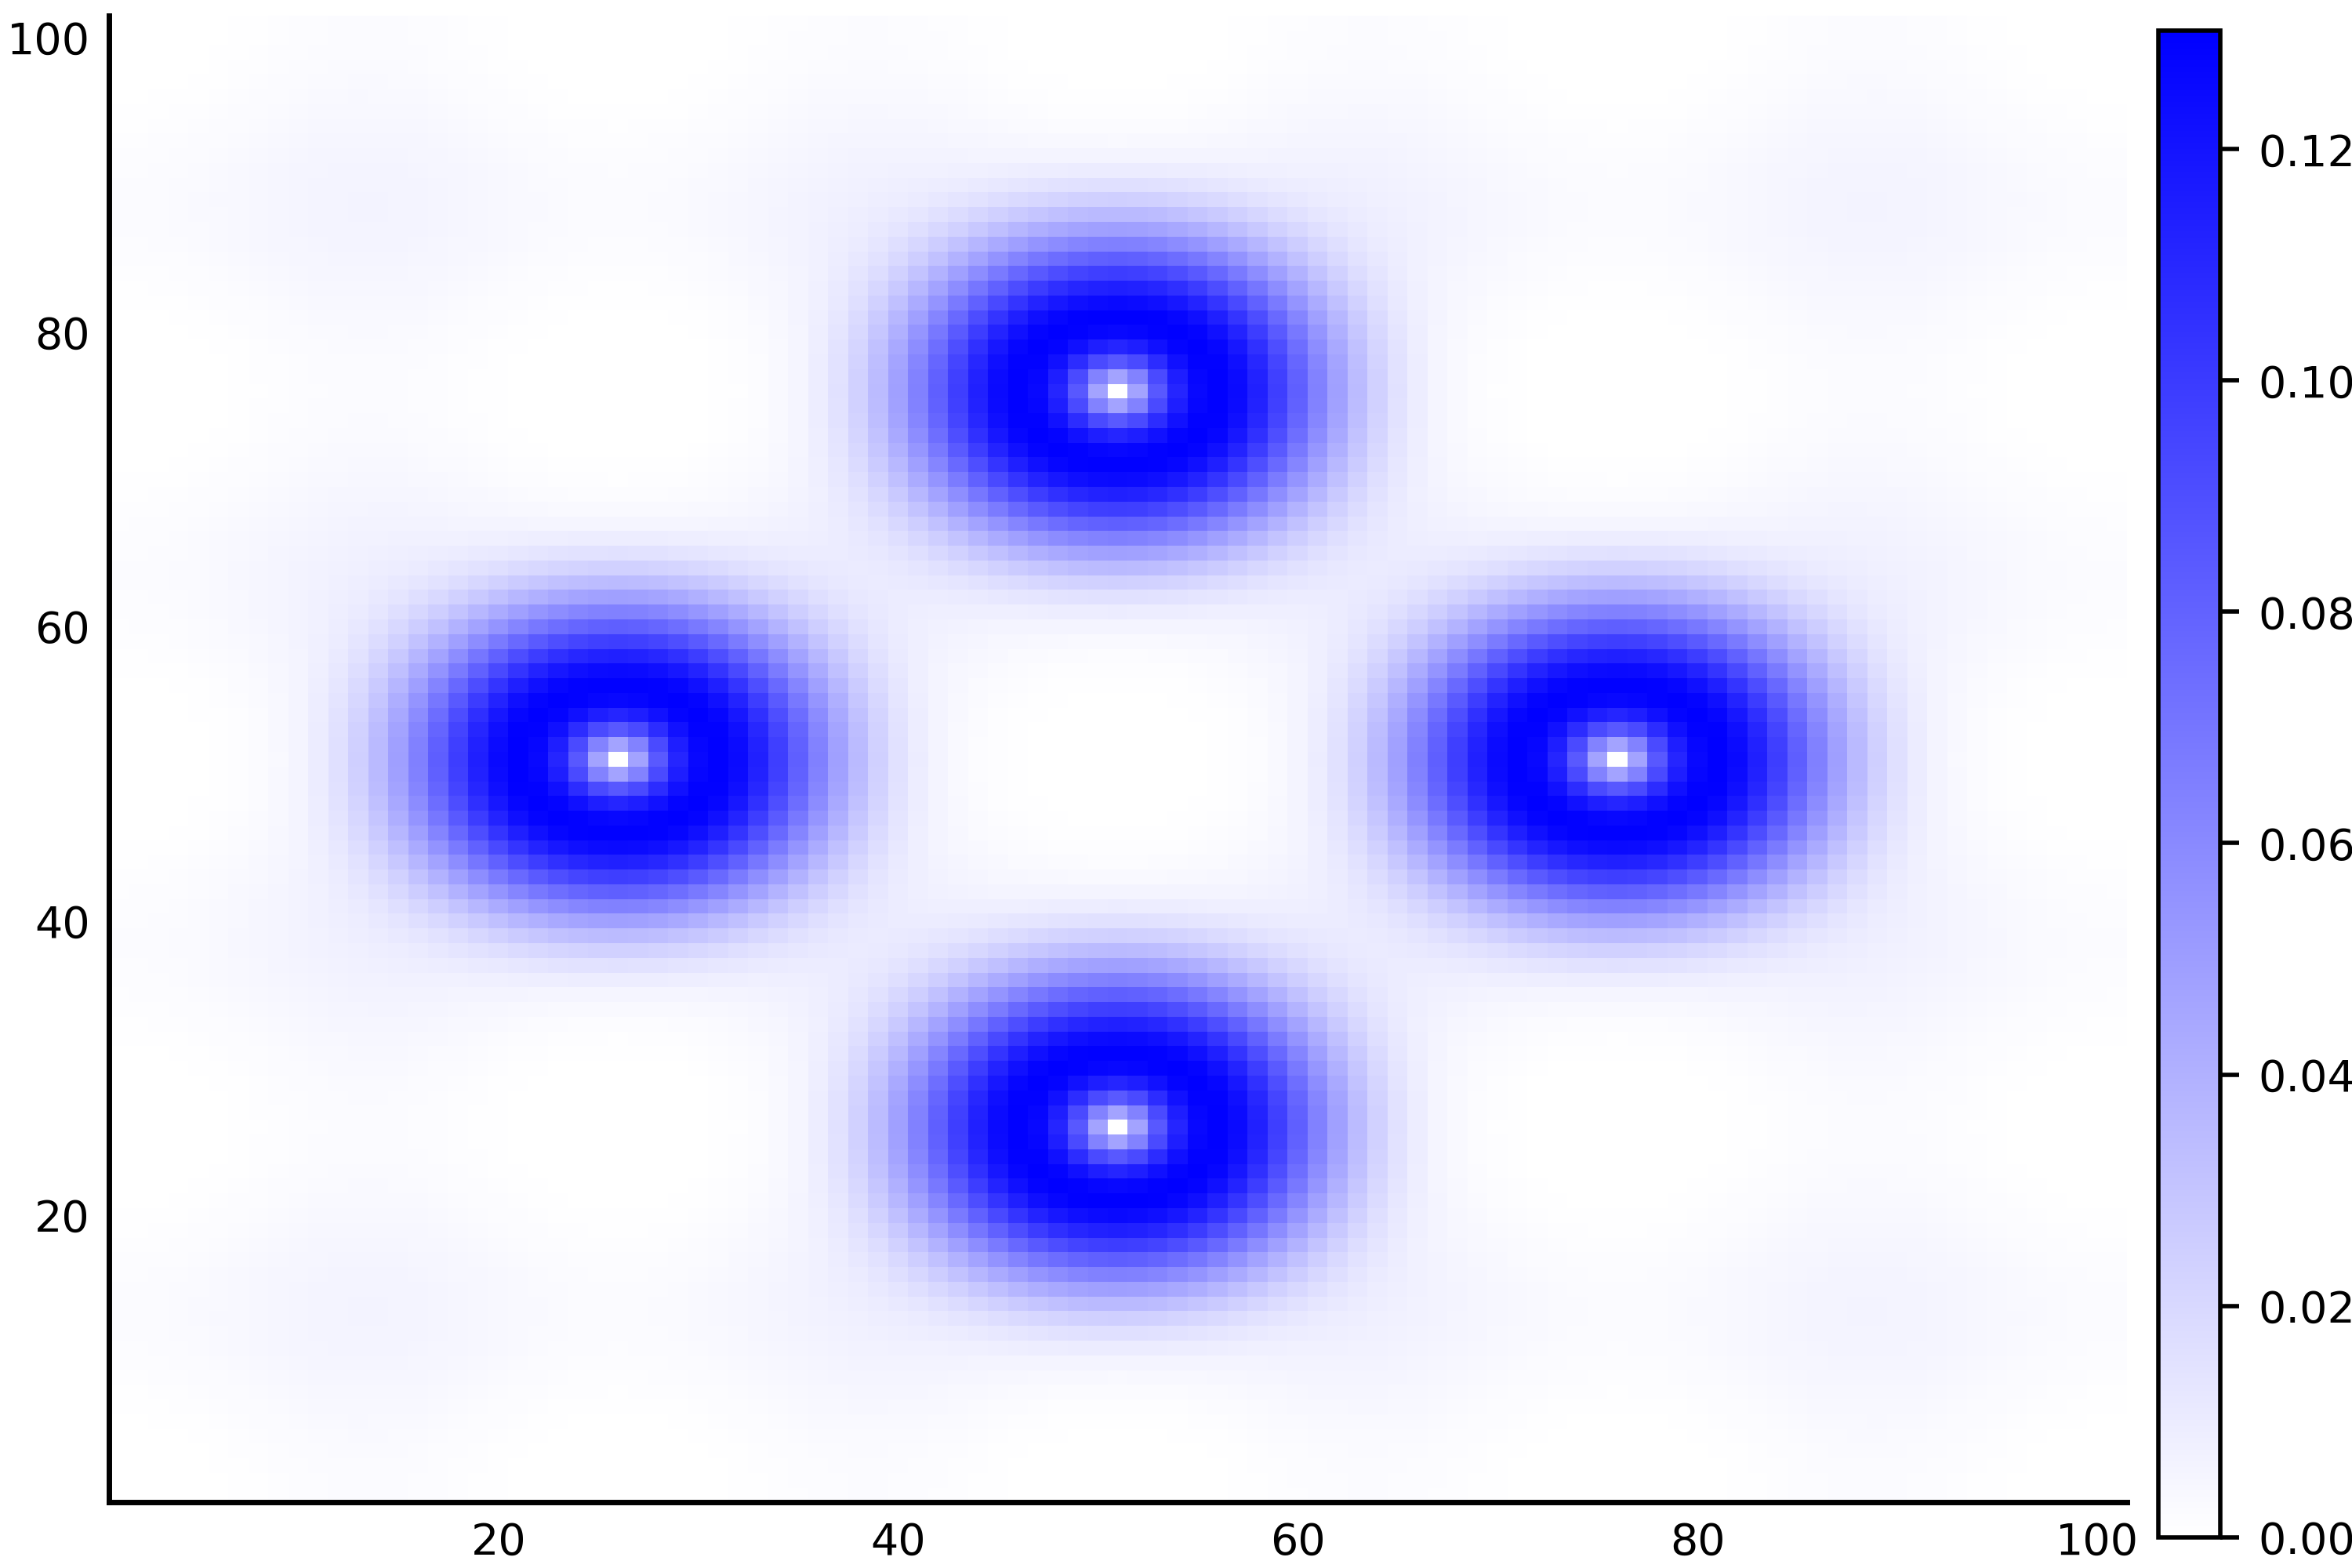
\includegraphics[scale=0.2]{figures/heatmaps/variance-mixture-25.png}} \\
    \hline
    \centering \textbf{Nonstationary length scale} &
      \parbox[c]{.18\textwidth}{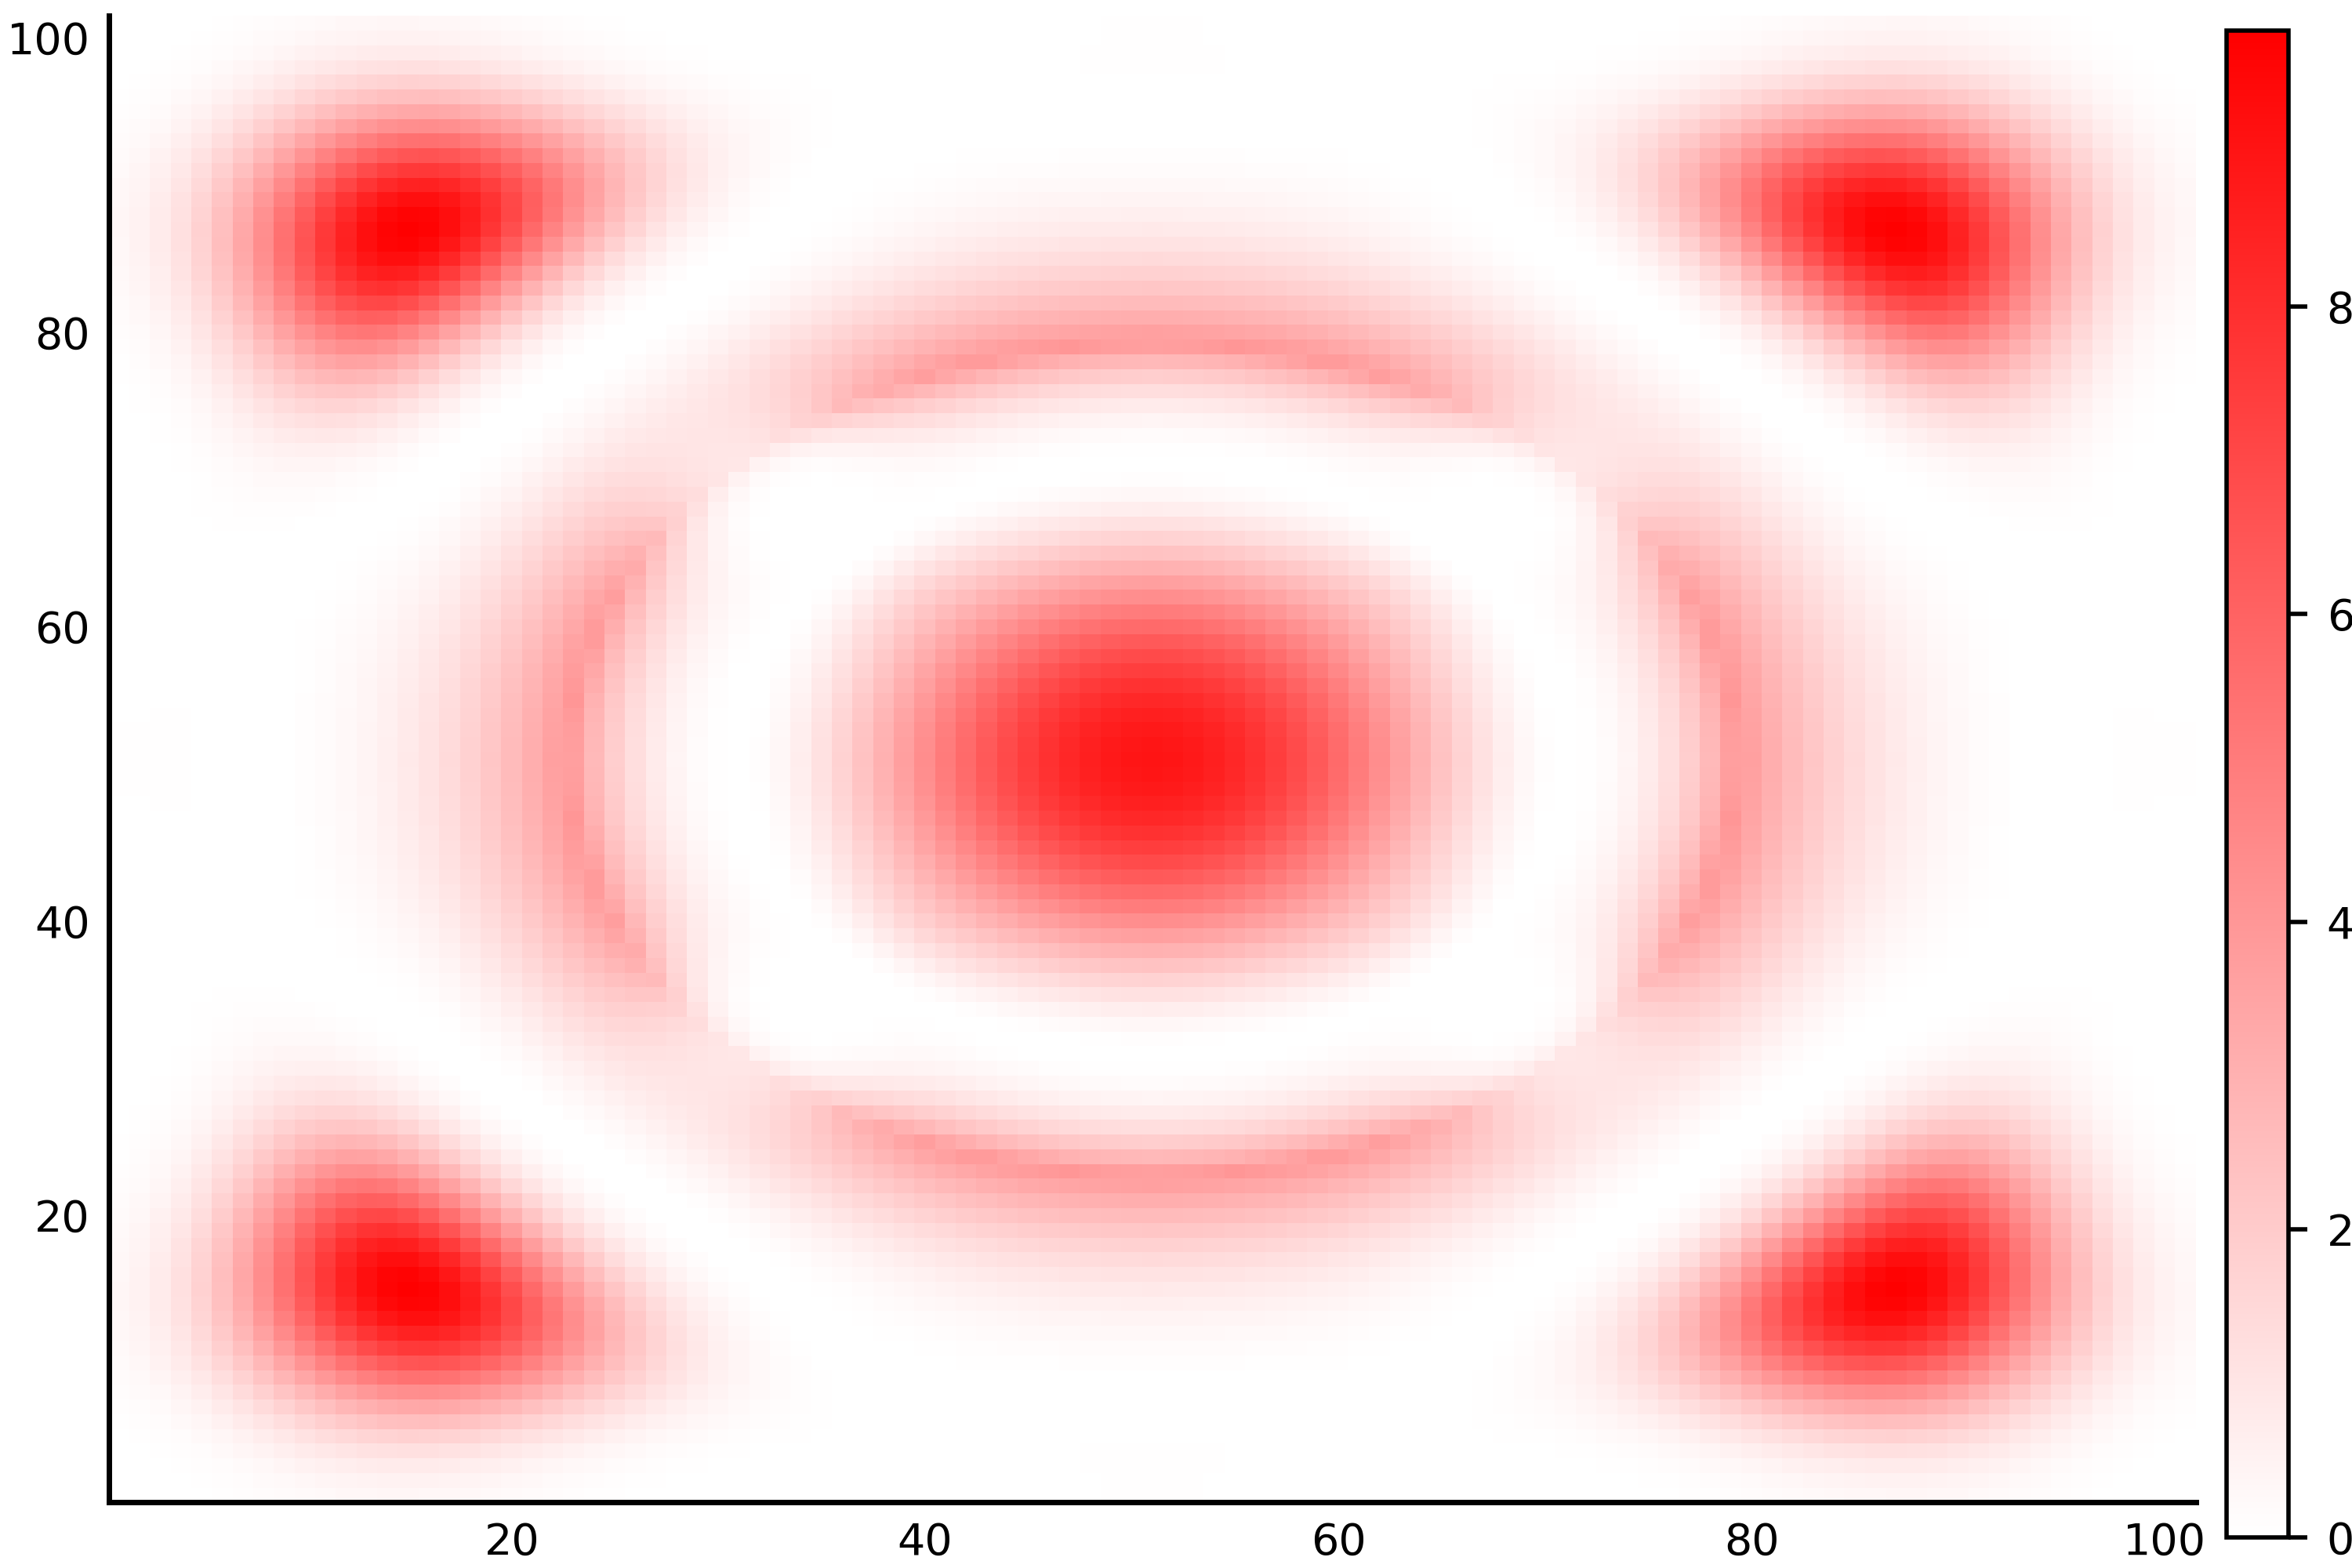
\includegraphics[scale=0.2]{figures/heatmaps/error-length-16.png}} &
      \parbox[c]{.18\textwidth}{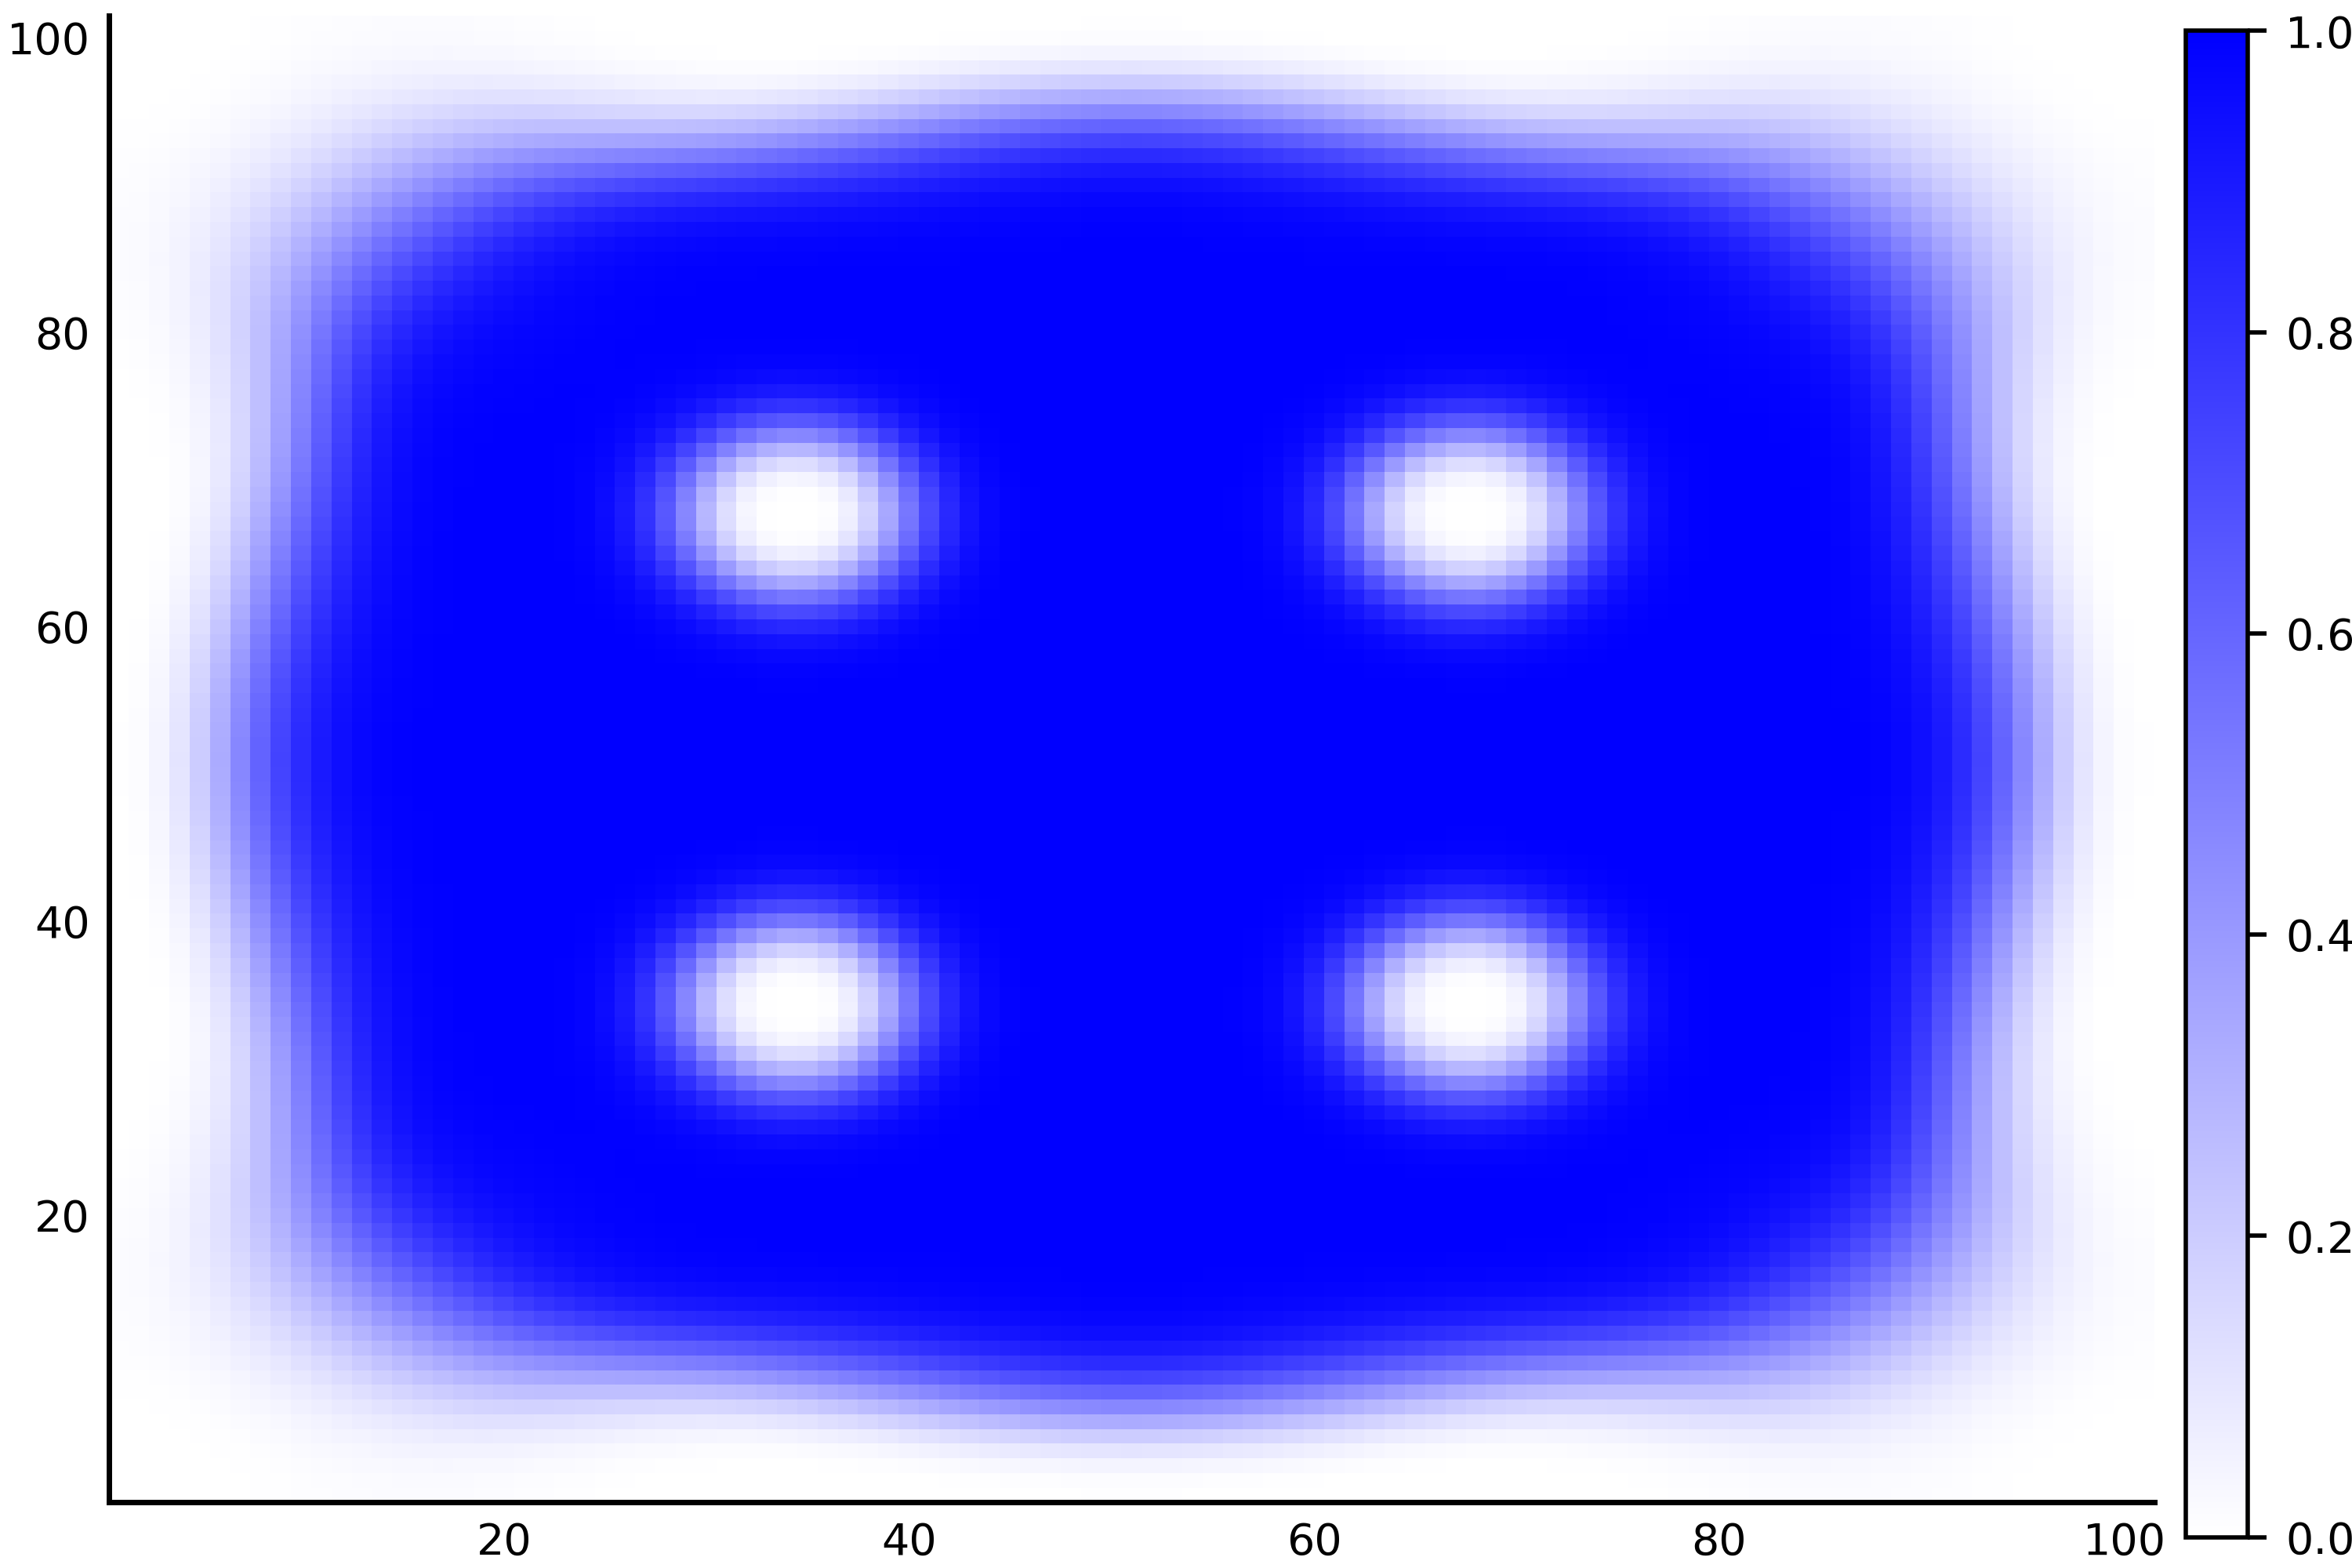
\includegraphics[scale=0.2]{figures/heatmaps/variance-length-16.png}} &
      \parbox[c]{.18\textwidth}{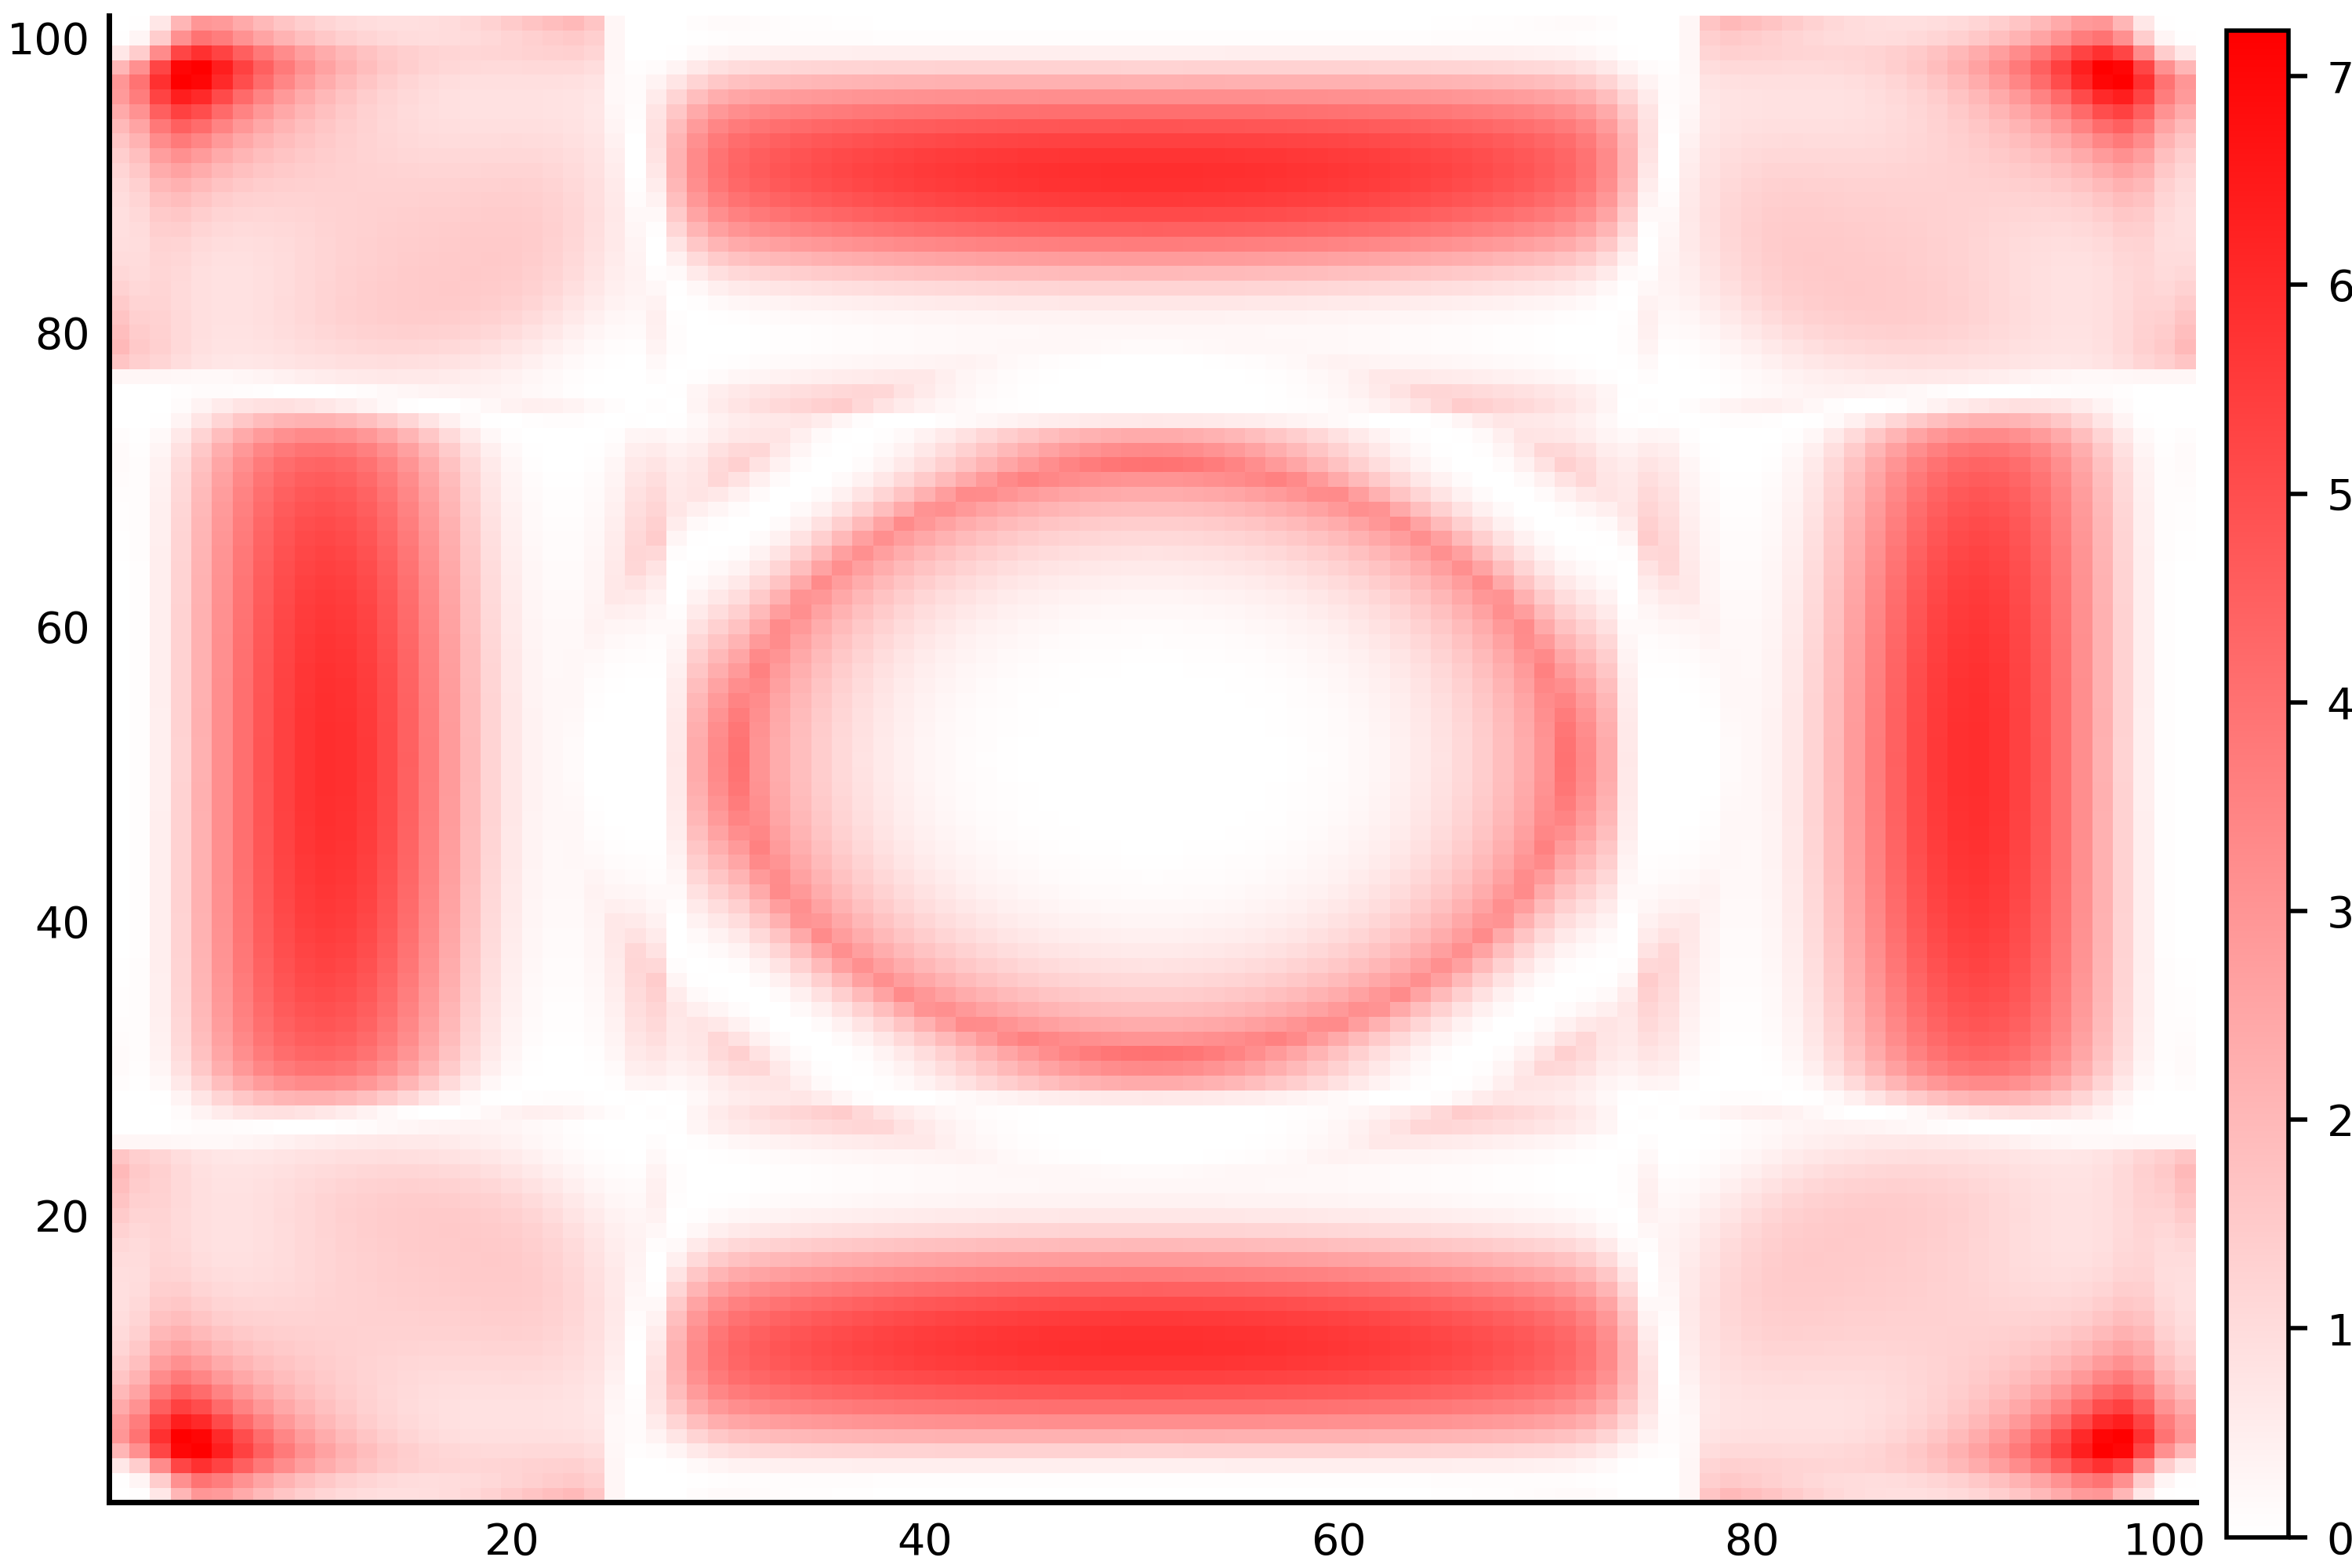
\includegraphics[scale=0.2]{figures/heatmaps/error-length-25.png}} &
      \parbox[c]{.18\textwidth}{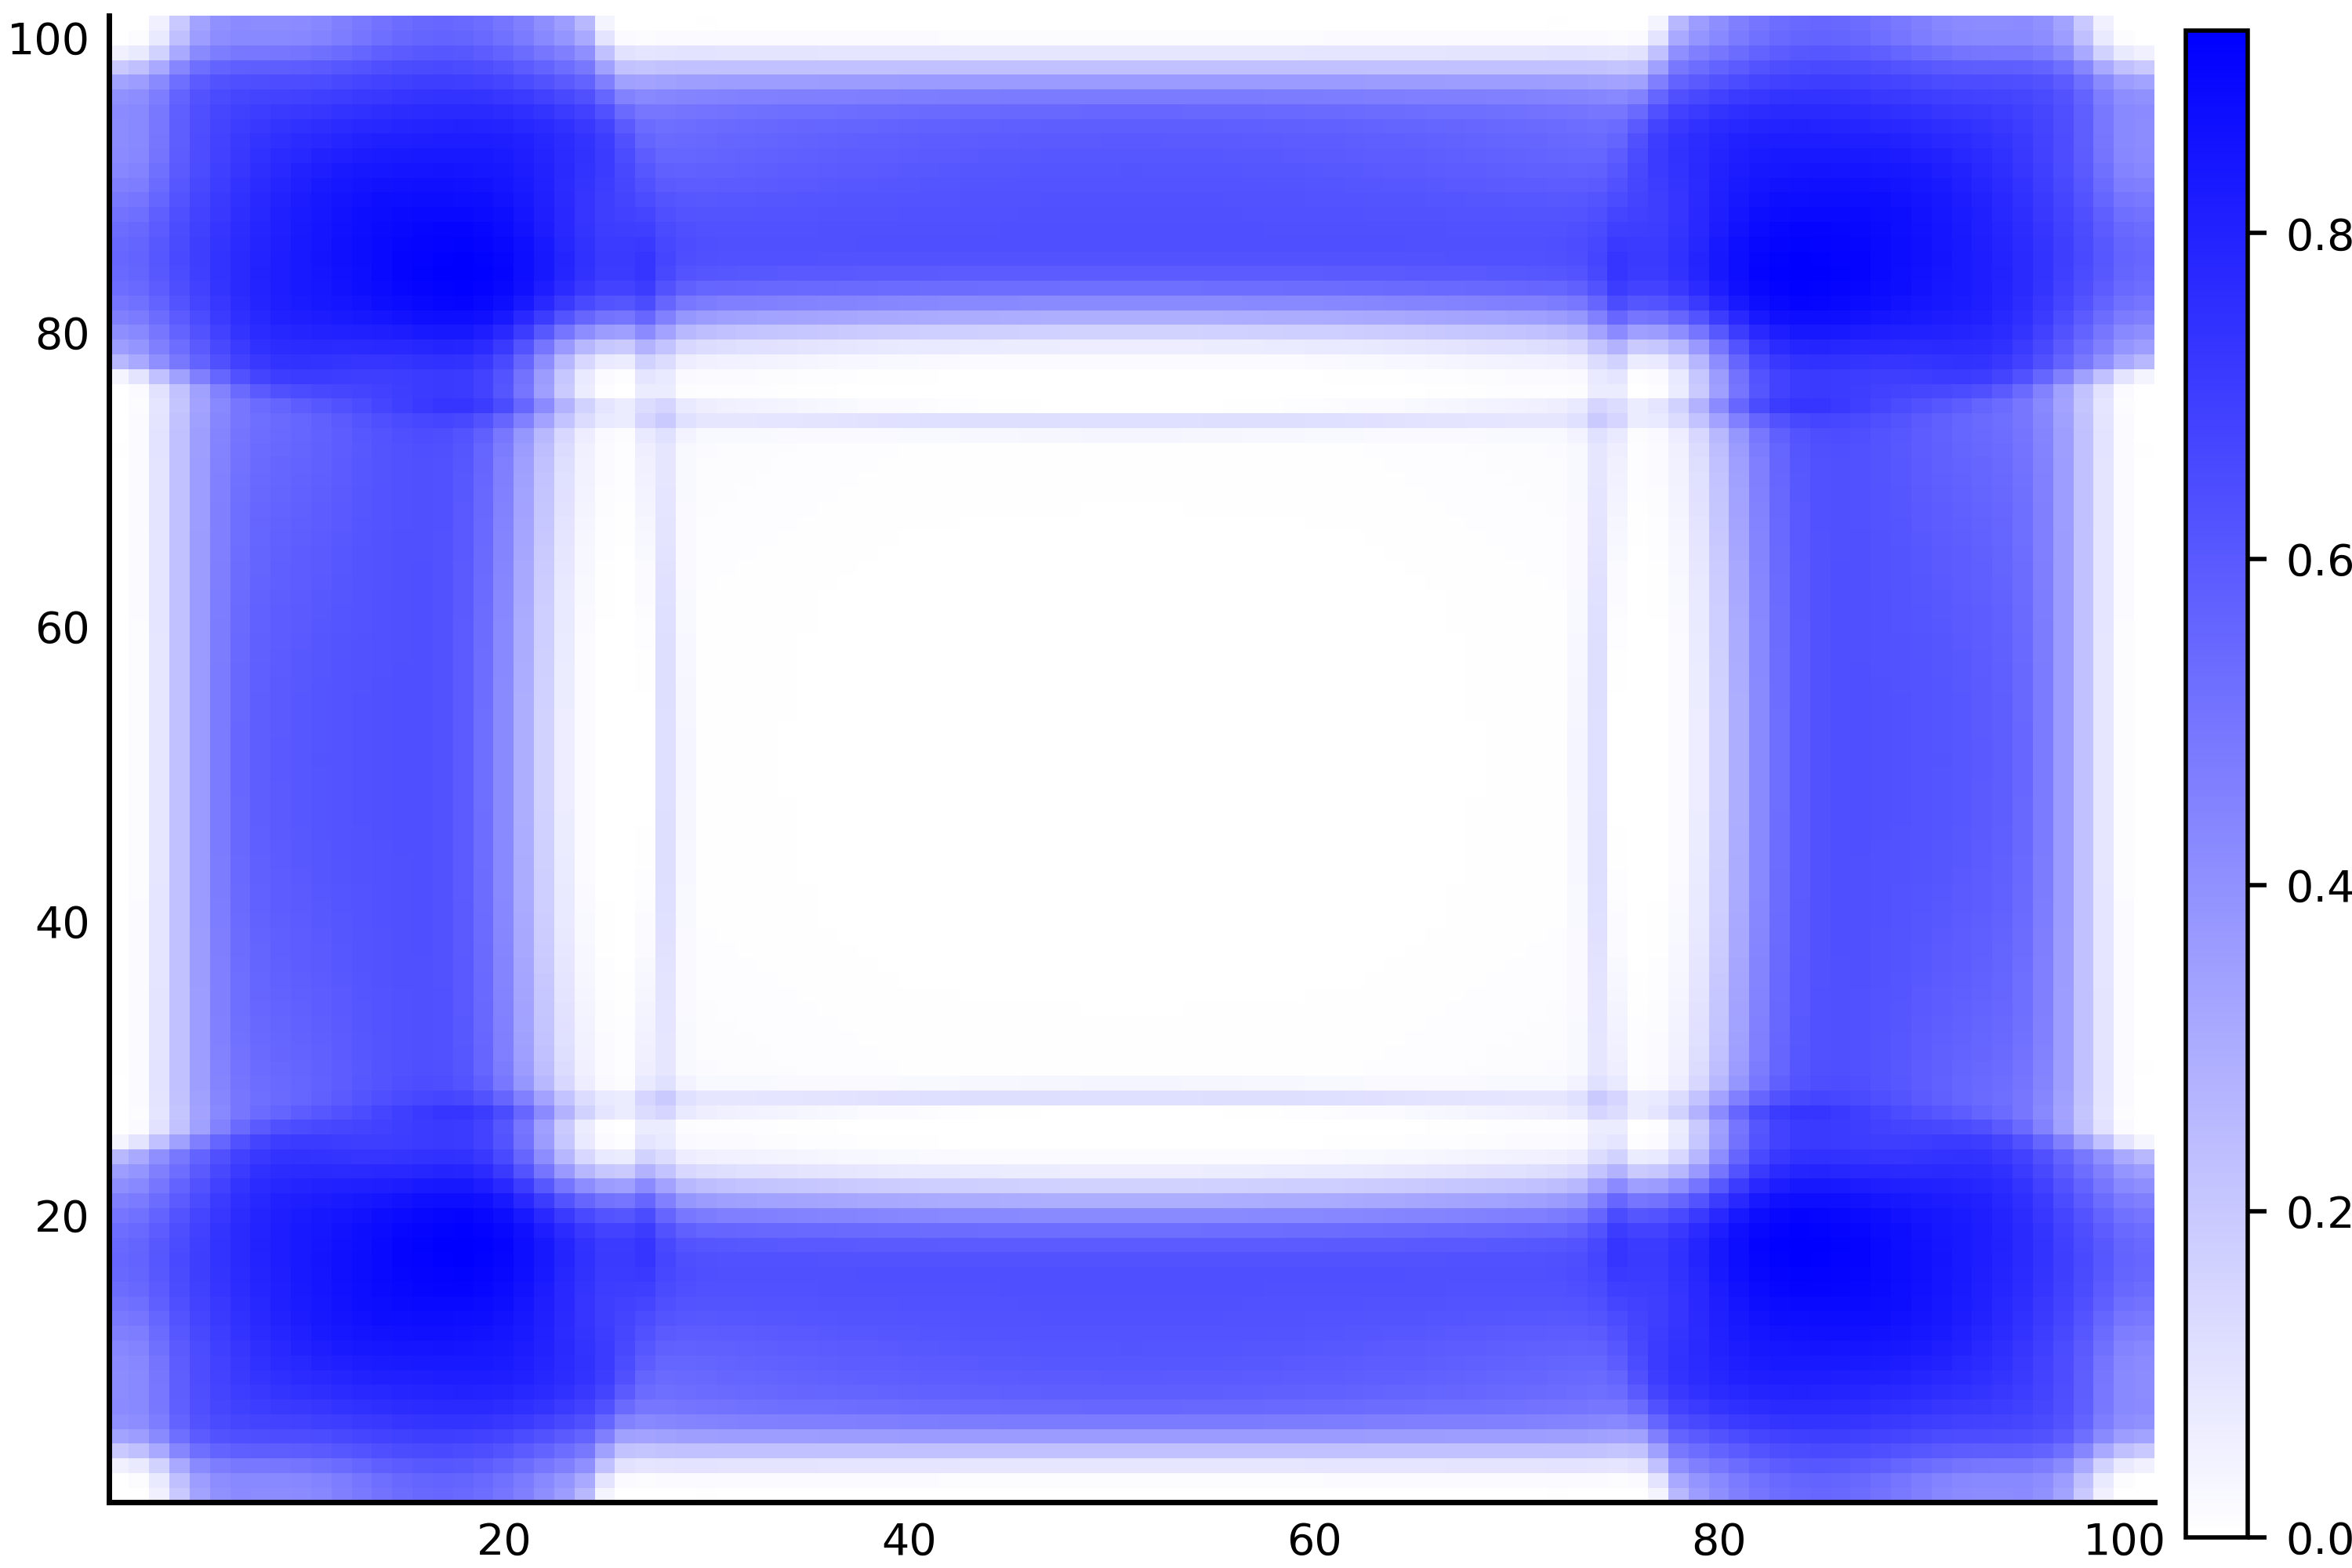
\includegraphics[scale=0.2]{figures/heatmaps/variance-length-25.png}} \\
    \hline
    \centering \textbf{Additive derivative noise} &
      \parbox[c]{.18\textwidth}{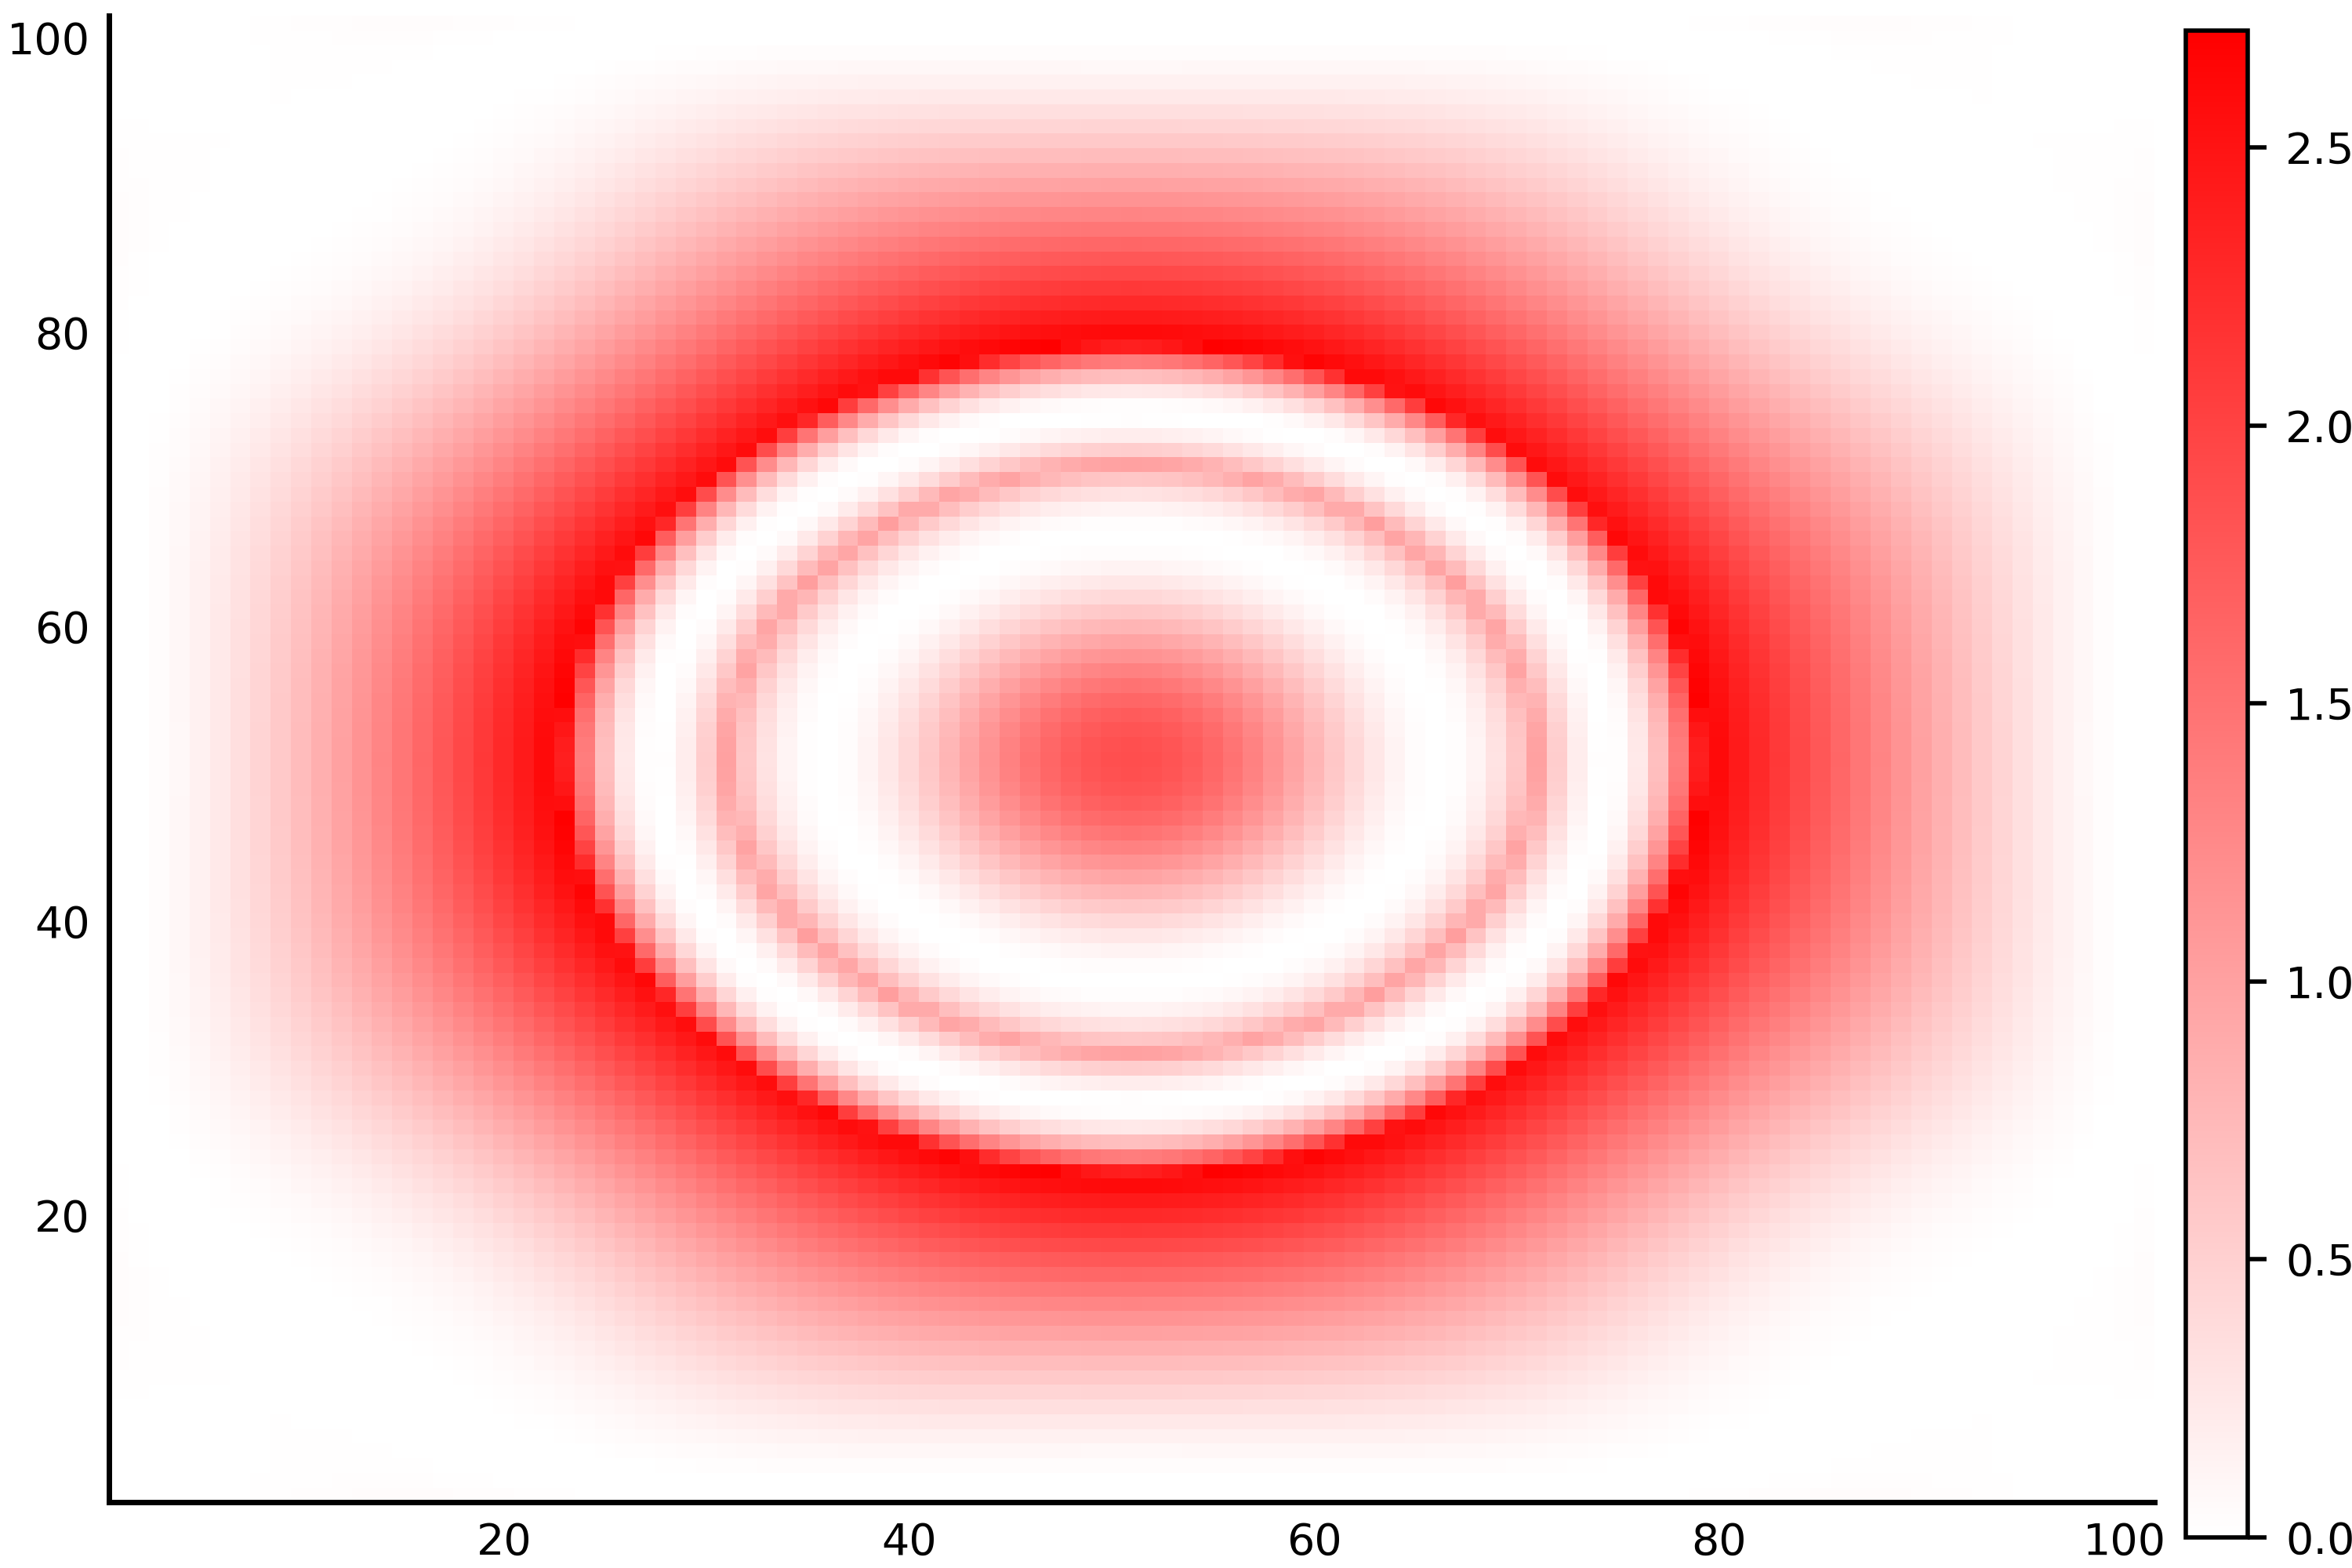
\includegraphics[scale=0.2]{figures/heatmaps/error-noisy-16.png}} &
      \parbox[c]{.18\textwidth}{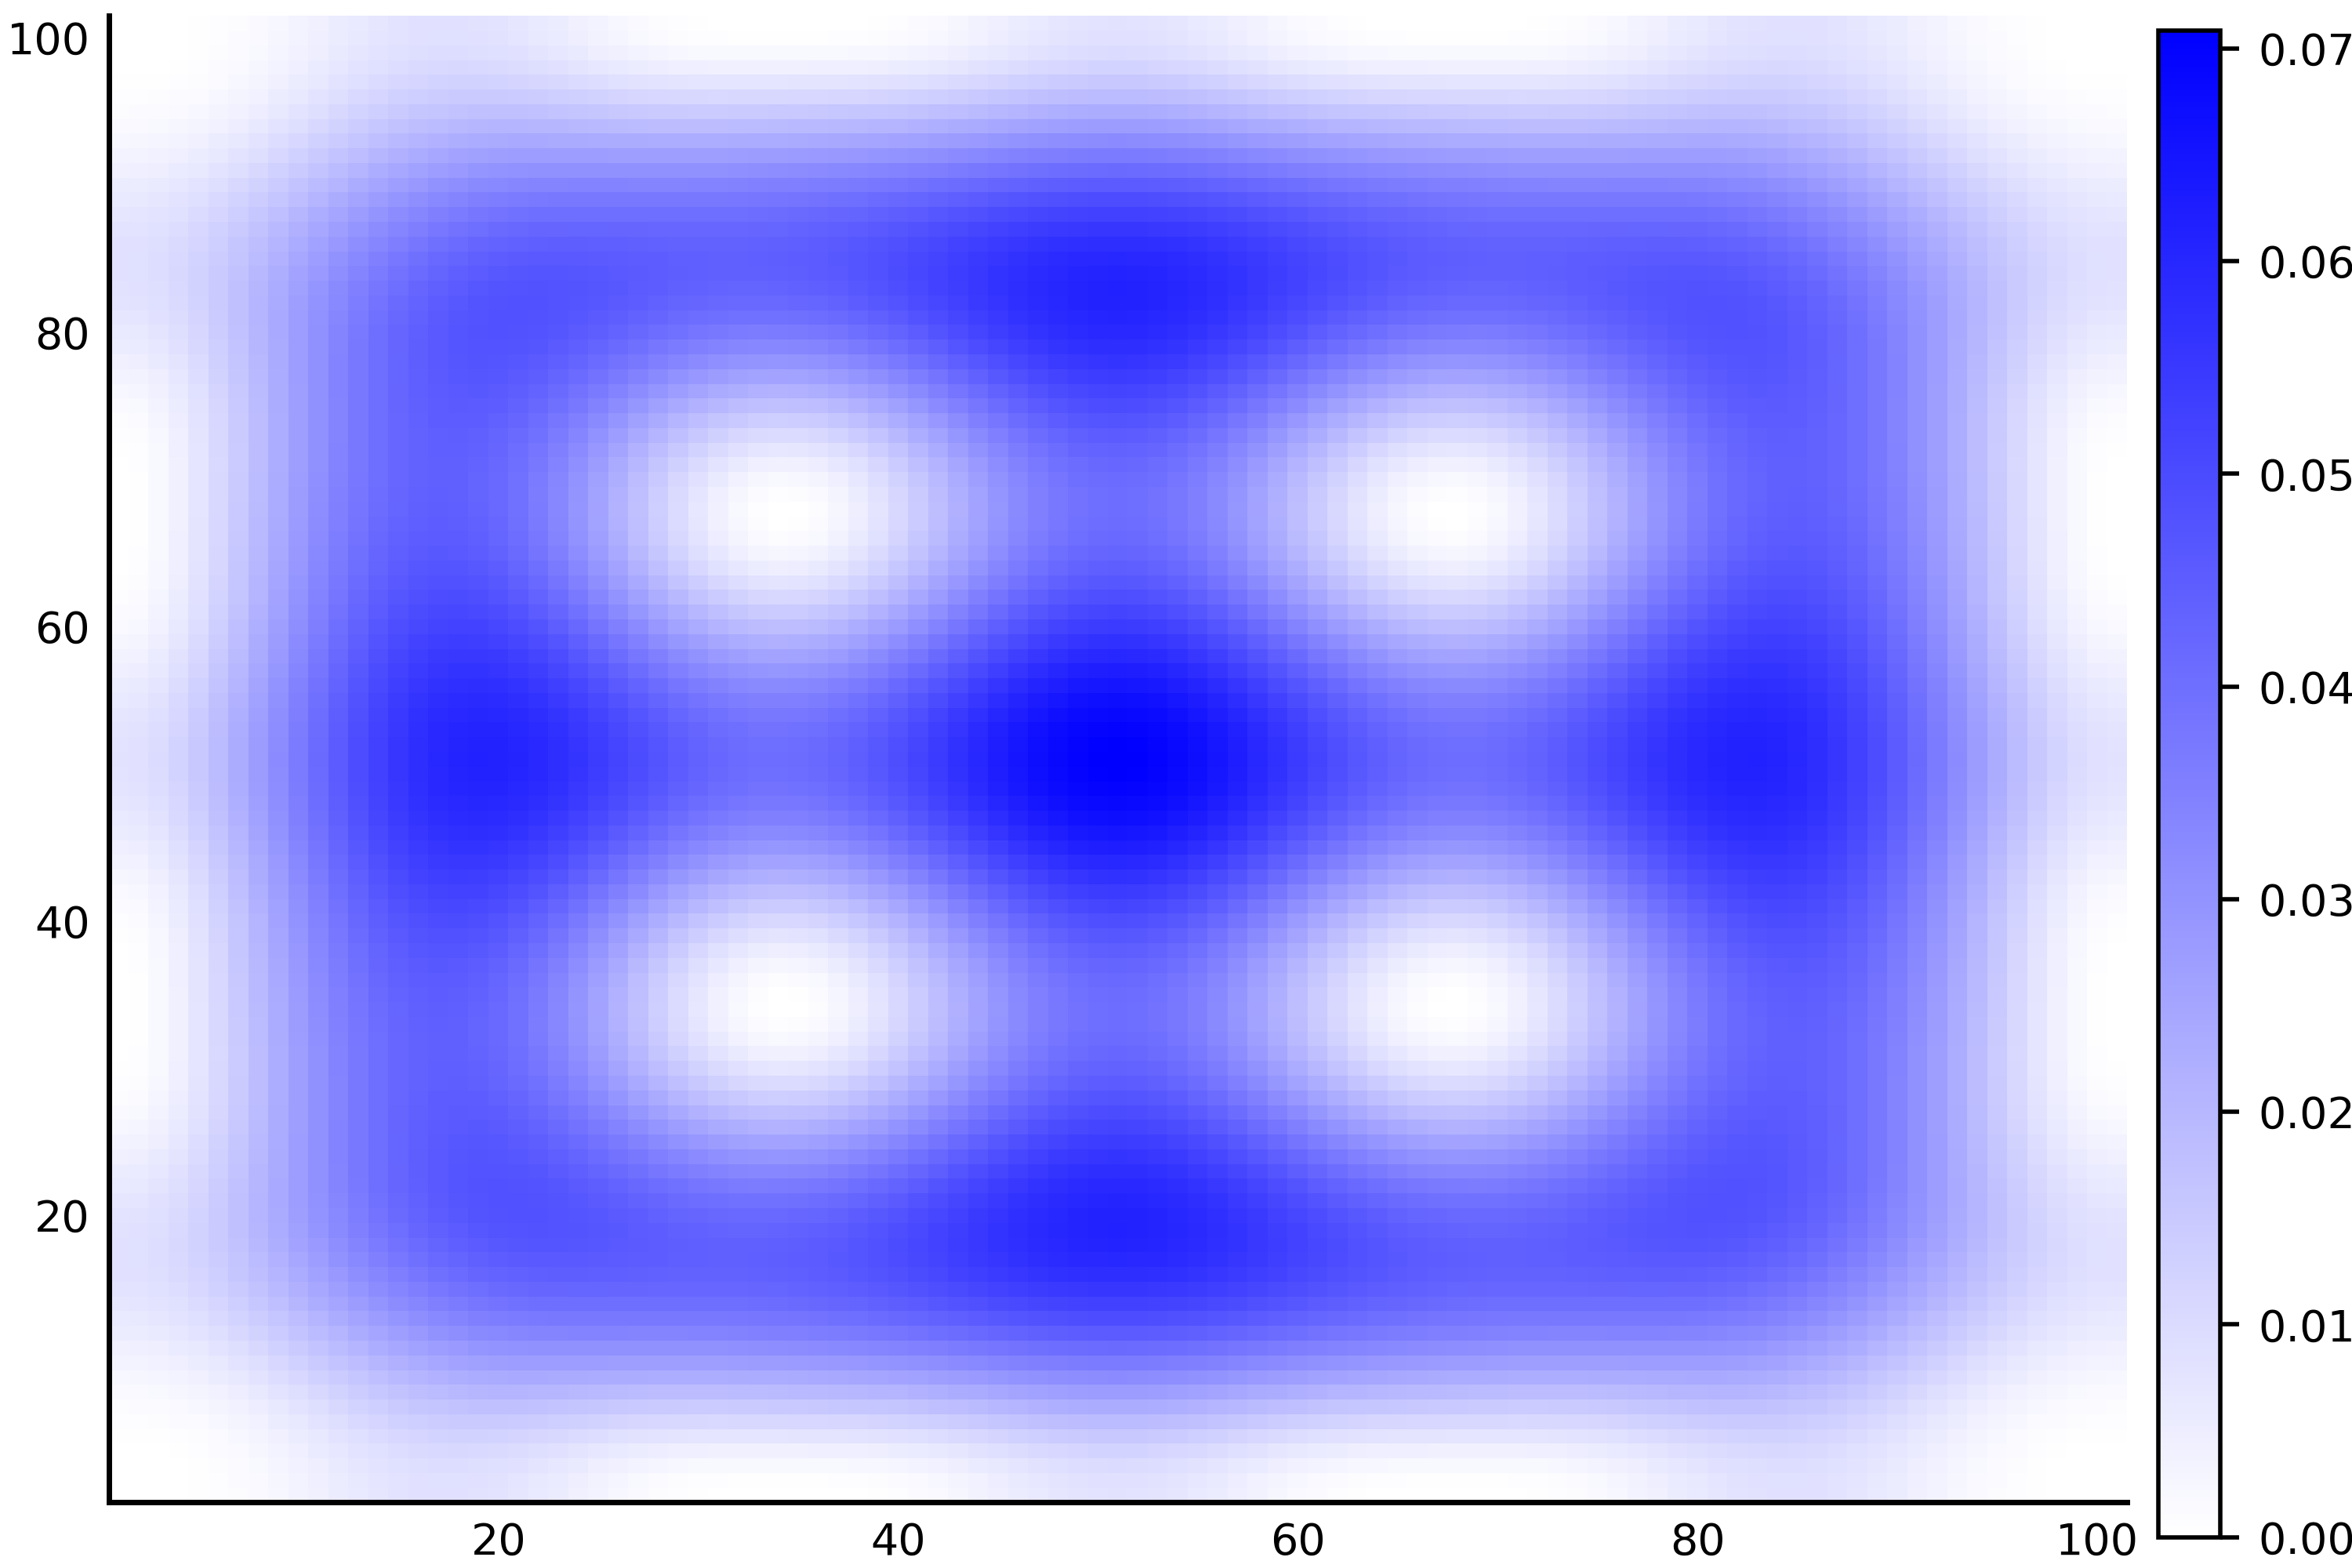
\includegraphics[scale=0.2]{figures/heatmaps/variance-noisy-16.png}} &
      \parbox[c]{.18\textwidth}{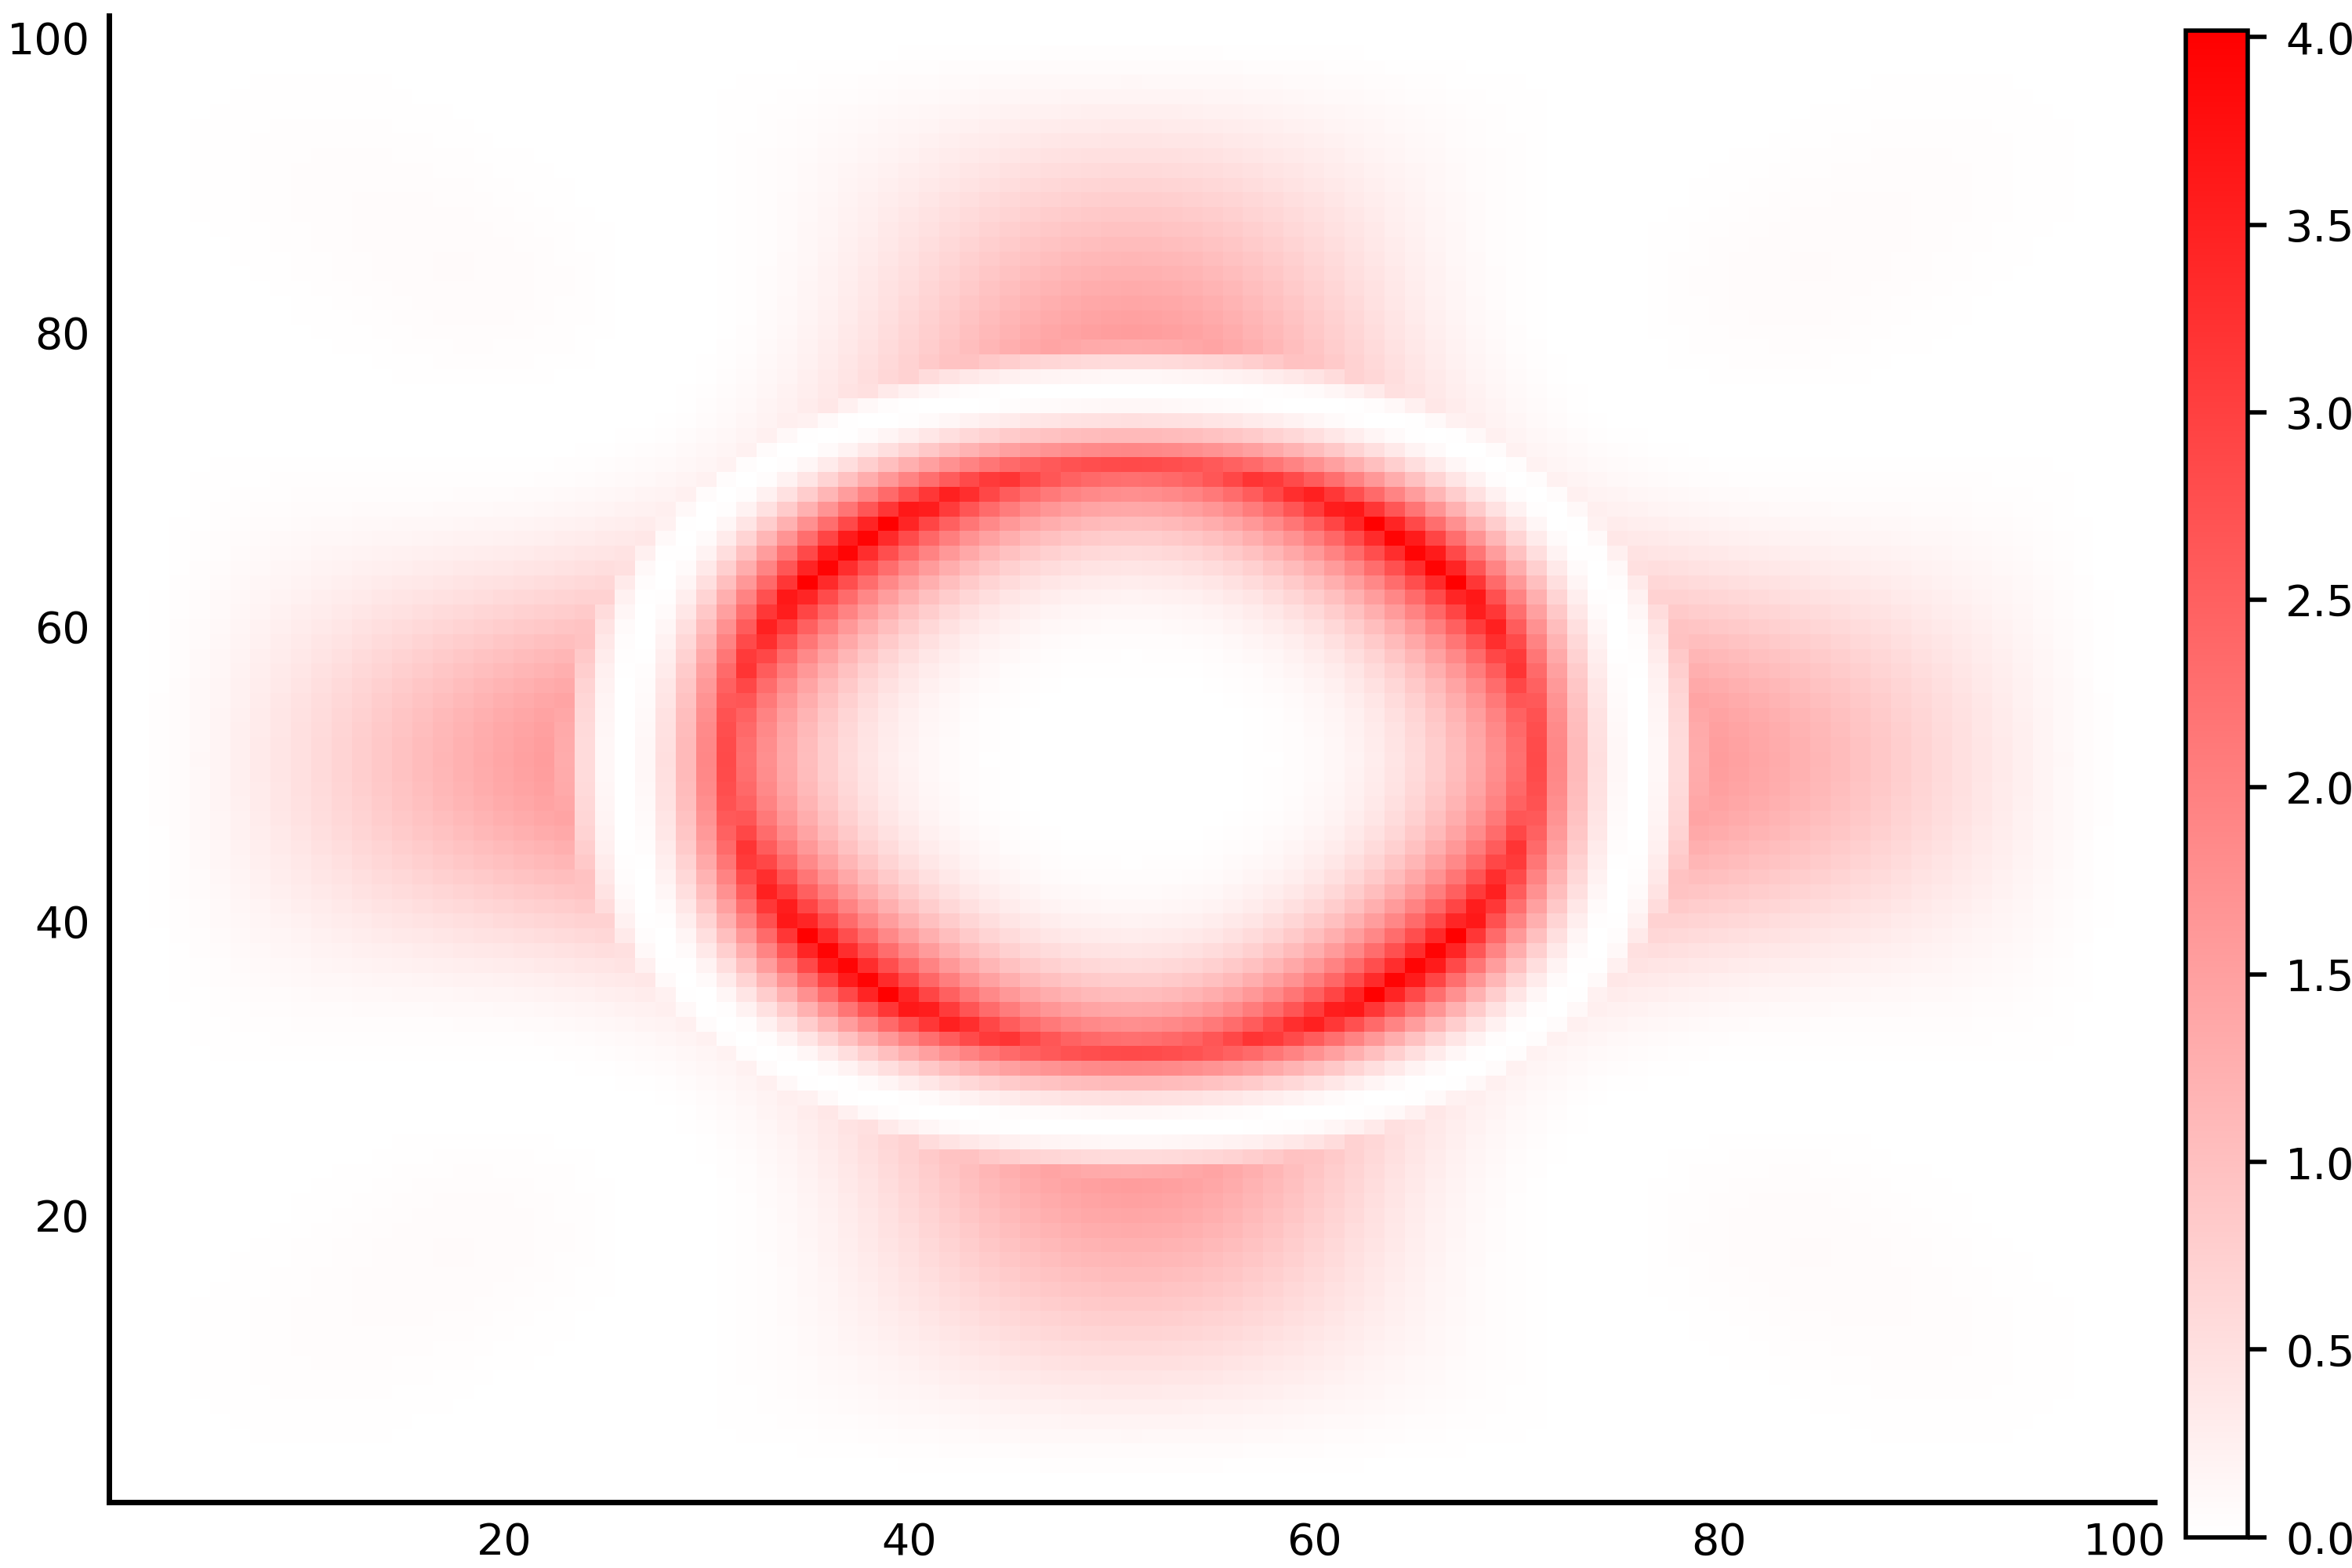
\includegraphics[scale=0.2]{figures/heatmaps/error-noisy-25.png}} &
      \parbox[c]{.18\textwidth}{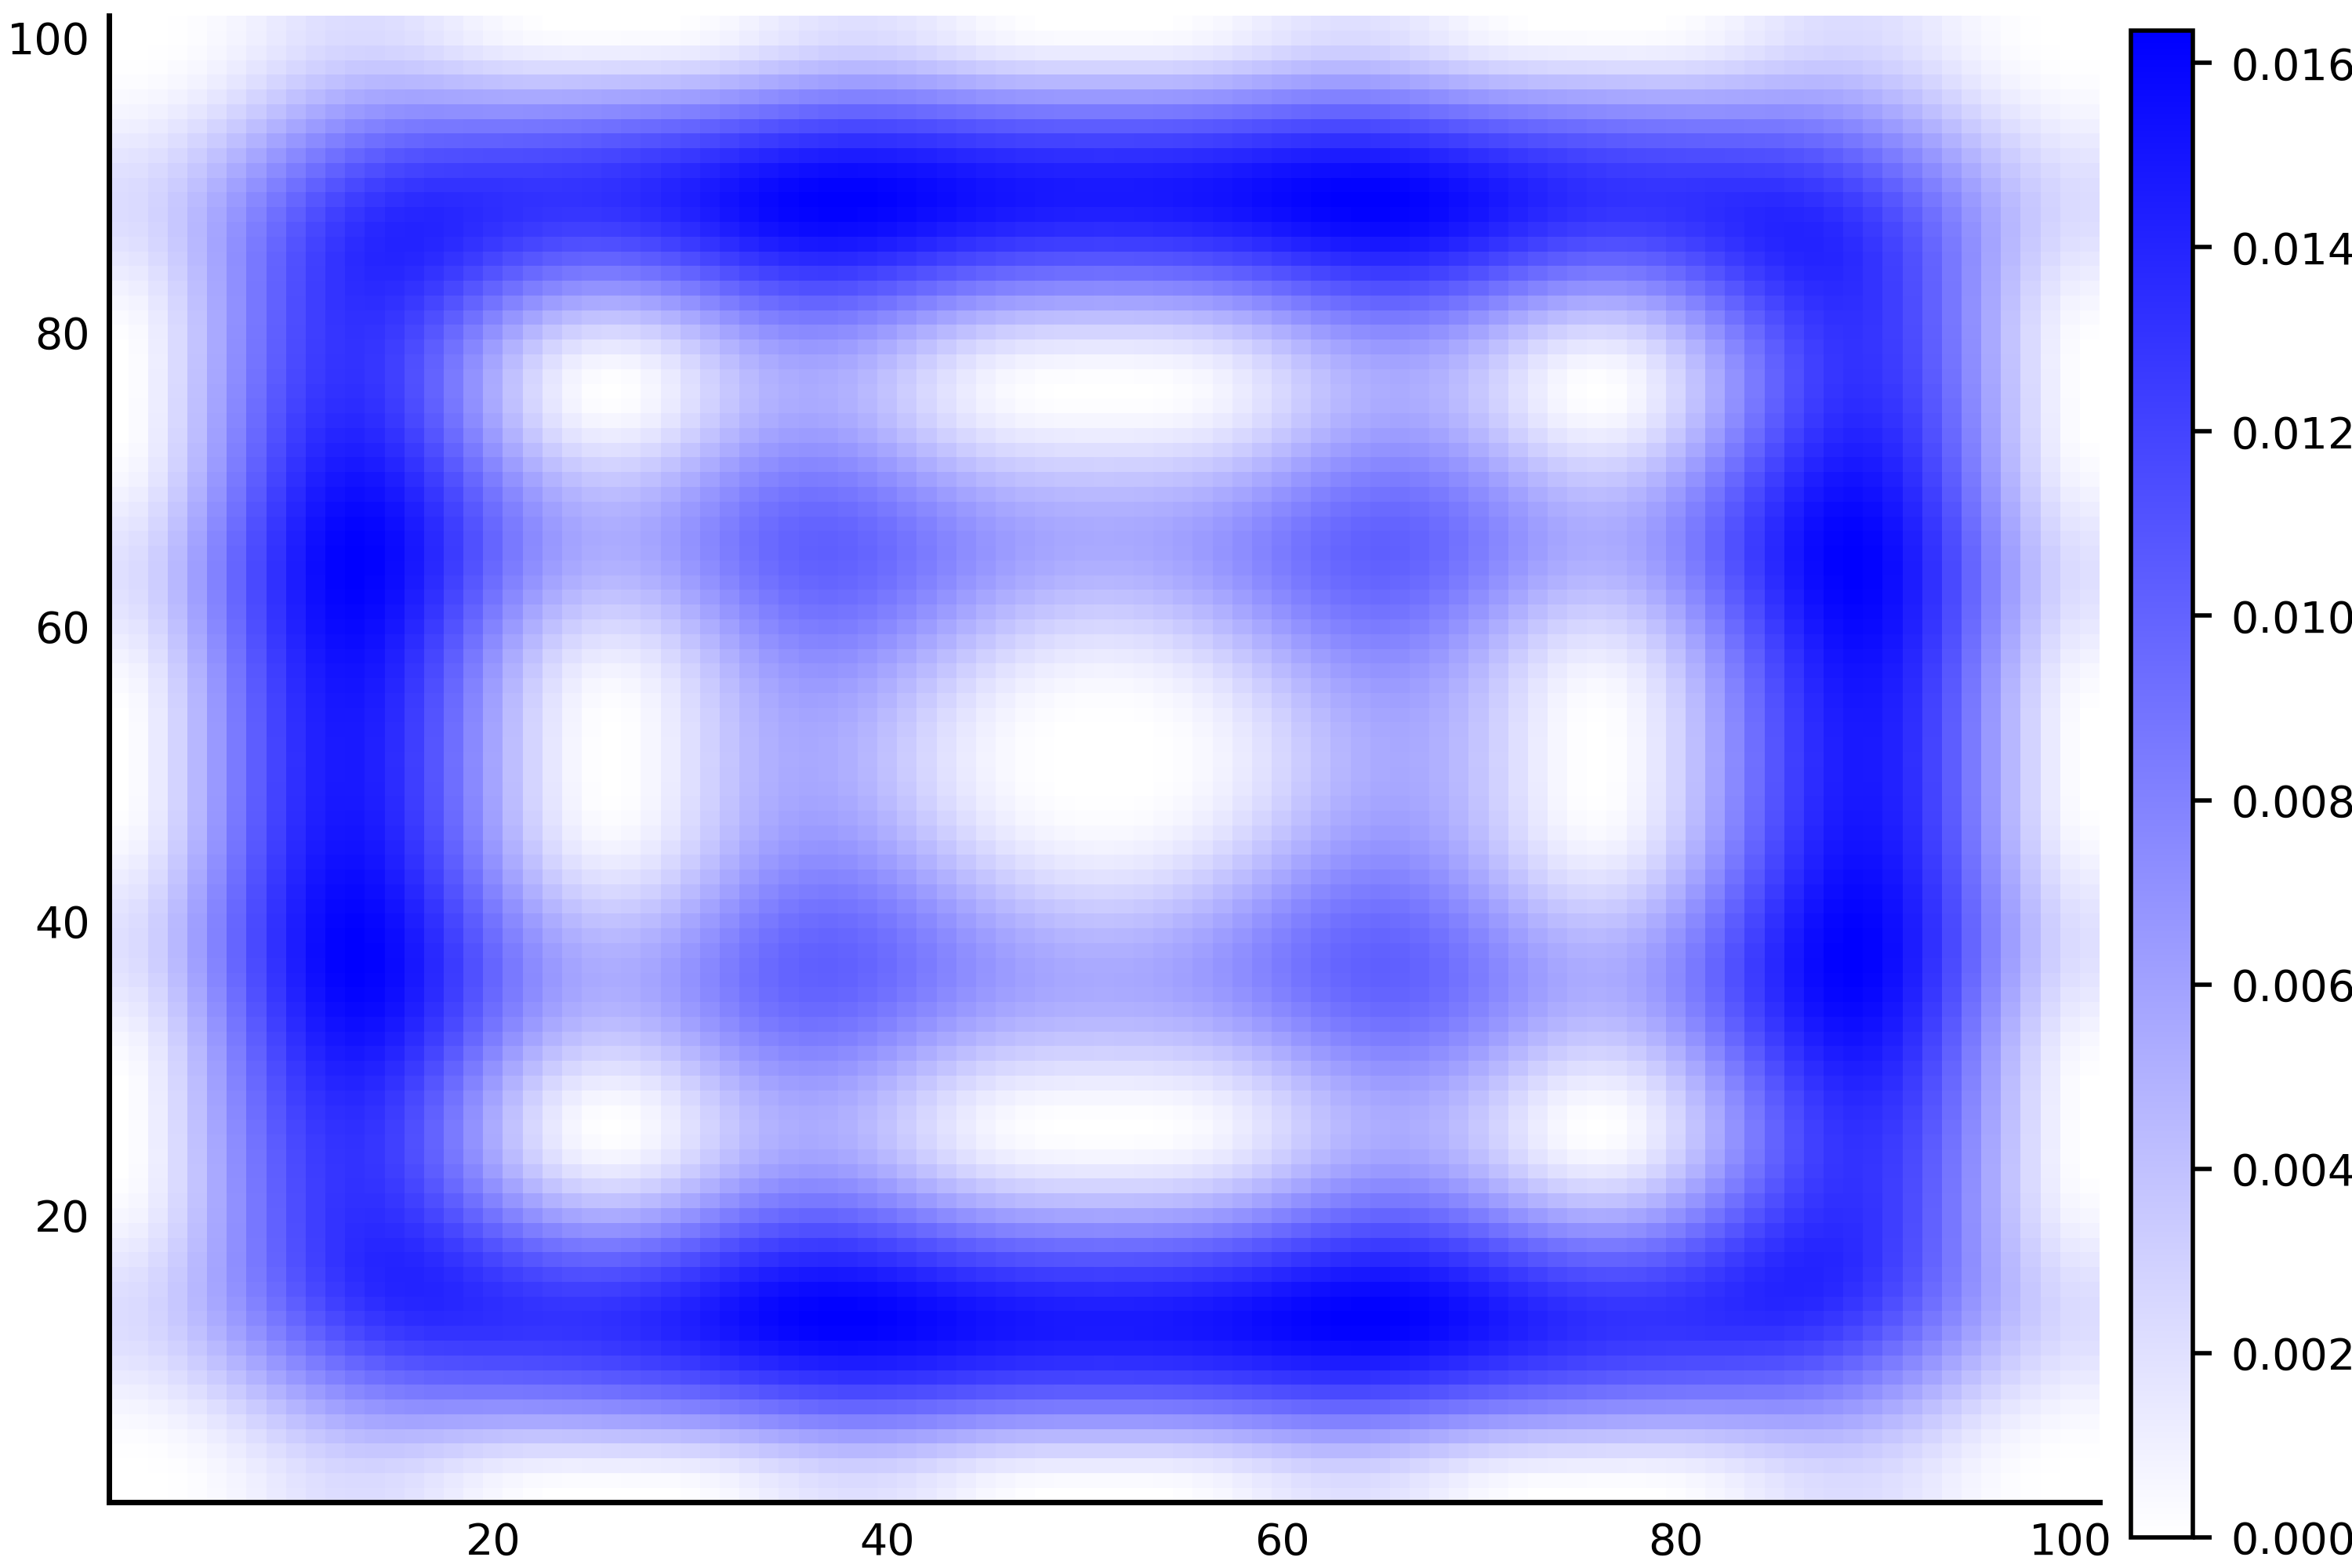
\includegraphics[scale=0.2]{figures/heatmaps/variance-noisy-25.png}} \\
    \hline
  \end{tabularx}
  \caption{Comparison of true error and variance for the radial test function in $\R^2$ using two regular grid designs. Error is show in red on the left of each panel, with the variance in blue on the right.}
  \label{variance}
\end{table}

\section{Conclusions}
Gaussian processes provide a powerful framework for interpolation of function and gradient values obtained from complex computer codes. In order to incorporate gradient observations obtained from automatic differentiation and to be used in optimization applications, a GP must use a twice differentiable kernel. However, for many codes of interest, nondifferentiabilities may arise in the function when the boolean value of conditional statements in the code changes. This results in a model misspecification problem, in which the true function is piecewise analytic while our approximation is everywhere twice differentiable. As a consequence of this misspecification, interpolating gradient observations near kinks can cause oscillation in the posterior mean.

We develop a method by which the distance to a potential kink is estimated using linear approximations constructed from function and gradient observations of the code's branching functions. We present a number of methods which use this branching distance data to introduce nonstationary effects which can improve our approximation near kinks. The following table provides a brief comparison of these methods.

\subsection{Comparison of methods}
\begin{center}
  \begin{tabularx}{\textwidth}{|p{.4\textwidth}|p{.26\textwidth}|X|}
    \hline
    \textbf{Method} & \textbf{Pros} & \textbf{Cons} \\
    \hline \hline
    \centering \textbf{Standard GP} & Does not suffer from oscillation near kinks & Requires many samples to generate accurate posterior \\
    \hline
    \centering \textbf{Gradient-interpolating GP} & Improved posterior accuracy in smooth regions & Oscillation near kinks \\
    \hline
    \makecell[t]{
      \textbf{Nonstationary smoothness} \\
      $\nu(\vec{x}) = \frac{1}{2} \exp\big(\min \frac{\hat{b}_k(\vec{x})}{\beta} \big)$
    } & Most appropriate model for the piecewise analytic functional class & Unable to interpolate gradient observations, nonstationary effects are isotropic \\
    \hline
    \makecell[t]{
      \textbf{Mixture of GPs} \\
      \parbox{.4\textwidth}{
        \begin{align*}
          p(c_i = 0 | \vec{x}_i) & = \left\{\begin{array}{lr}
                      1 & \text{for } \min \hat{b}_k(\vec{x}_i) < \varepsilon \\
                      0 & \text{otherwise} \qquad
                    \end{array} \right \\
          p(c_* = 0 | \vec{x}_*) & = s\Bigg(\min_{\substack{x_i \in X \\ c_i = 0}} \norm{\vec{x}_* - \vec{x}_i}\Bigg)
        \end{align*}
      }
    }
    & Interpolates gradient observations in smooth regions with appropriately increased uncertainty in nonsmooth regions & Posterior is nondifferentiable near kinks \\
    \hline
    \makecell[t]{
      \textbf{Nonstationary length scale} \\
      \parbox{.4\textwidth}{
        \small{
          \ell_k(\vec{x}) = (\ell_{max} - \ell_{min}) \big[1 - \exp\big(-\frac{\hat{b}_k(\vec{x})}{\beta}\big)\big] + \ell_{min}
        }
      }
    } & Nonstationary effects are anisotropic, posterior is everywhere differentiable, variance increased near kinks & Sensitive to hyperparameter selection, computing the posterior mean of $p$ directional branching distance GPs is a bottleneck in higher dimensions \\
    \hline
    \makecell[t]{
      \textbf{Additive derivative noise} \\
      $\sigma^2_k(\vec{x}_i) = \sigma^2_{max} \exp\big(- \frac{\hat{b}_k(\vec{x}_i)}{\beta}\big)$
    } & Computationally efficient, nonstationary effects are anisotropic, posterior is everywhere differentiable & Variance underestimates error near kinks \\
    \hline
  \end{tabularx}
\end{center}

\subsection{Recommendations}
Our additive derivative noise model demonstrates superior accuracy and stability in our numerical tests when compared to alternative methods, and in particular shows significant improvement over standard GPs for low sample densities while avoiding the oscillation problems of gradient-interpolating GPs. The domain of low sample density is highly relevant in optimization of expensive computer codes, as the number of function evaluations is limited. We believe that the accuracy and stability benefits seen for low sample densities may allow sequential optimization algorithms to identify regions of interest more effectively using small initial designs, leading to faster convergence. Given our promising numerical results on synthetic test functions, we hope to further investigate the analytical properties and numerical performance of our additive derivative noise model in larger scale computer code modeling applications.

\section{Future work} \label{future-work}
In order to determine the effectiveness of our additive derivative noise model in practical applications, we hope to extend an AD tool in C++ to supply the branching function values and gradients. When this is complete, we can validate our method against function-interpolating and gradient-interpolating GPs in higher dimensions both by computing the ISE and observing convergence rates in sequential optimization contexts.

Another concern in approximating branching distance in more complex codes is whether or not a given branching function $g_j$ is \textit{active} for an input $\vec{x}$, that is whether $\vec{x}$ lies in a subdomain bounded by the zero level-set of $g_j$. For example, for $\vec{x}$ in the outer ring $\norm{\vec{x}}_2^2 > 2$ of \texttt{rad1}, the value of the inner branching function $\norm{\vec{x}}_2^2 - 1$ should be irrelevant to $\hat{b}_k(\vec{x})$ as it will never cause a kink. Distinguishing between active and inactive branching functions should be studied further when implemented in an AD tool.

A final area for further work is determining how construct the nonstationary noise matrix $\Sigma(X)$ to minimize error, either by optimizing the hyperparameters in its current exponential form, or deriving an improved functional form. Common methods for parameter estimation of GPs include maximum likelihood estimation and cross validation~\cite{rasmussen2003gaussian}. Comparing the effectiveness of these and other methods would facilitate the use of our nonstationary methods when reasonable hyperparameters are not known a priori.

A more general framework for error analysis of Gaussian processes is the \textit{generalization error}~\cite{rasmussen2003gaussian, sollich1999learning}, which gives the expected loss when the set of inputs $X^{(n)}$ are drawn from a distribution over the input space $\Omega$ and the true function $f$ is drawn from a prior over a functional space $\mathcal{F}$. Using loss function $\mathcal{L}(\cdot, \cdot)$, the generalization error using $n$ data points is given by
$$ E(n) = \int \int \int \mathcal{L}\Big(f(\vec{x}), \hat{f}(\vec{x})\Big) p(\vec{x}) p(f) p\big(X^{(n)}\big) \, d\vec{x} \, df \,  dX^{(n)},$$
where $\hat{f}$ is the posterior mean of a GP. This form gives a conceptually straightforward method for studying average-case convergence under model misspecification as we have between piecewise analytic functions and twice differentiable GPs, since we can chose the space $\mathcal{F}$ from which the true function is selected to have a smoothness level different from that of the estimator $\hat{f}$. Studying the ISE is a first step towards addressing this error, as the ISE results from taking $E(n)$ when $f$ and $X^{(n)}$ are fixed, $p(\vec{x})$ is uniform, and the $\ell_2$ loss is used. We believe that further work studying the ISE and the generalization error may lead to improved functional forms for nonstationary effects.

\newpage

\bibliography{refs}{}
\bibliographystyle{plain}

\end{document}
